% !TEX encoding = UTF-8 Unicode
% !TEX TS-program = lualatex
% !BIB TS-program = biber



\begin{filecontents*}{\jobname.xmpdata}
\Author{Giacomo Garaccione}
\Title{Advancing Software Engineering Practices through Gamification and Automated Techniques}
\Subject{Doctoral dissertations in the SCUDO doctoral school}
\Keywords{PDF\sep
          PDF/A\sep
          ISO 19005\sep
          LaTeX\sep
          PhD Thesis\sep
          Engineering\sep
          SCUDO}
\Publisher{Politecnico di Torino}
\end{filecontents*}


\documentclass[12pt,   twoside,   tipotesi=scudo,   numerazioneromana]{toptesi}
\usepackage{toptesi}
\usepackage{comment}
\usepackage[loadshadowlibrary]{todonotes}
\usepackage{listings}
\usepackage{xcolor}
\usepackage{subcaption}
\usepackage{soul}
\usepackage{tcolorbox}
\usepackage{palatino}

\usepackage{fancyhdr}
\usepackage{fancybox}
\usepackage{fancyvrb}
\usepackage{colortbl}
\usepackage[hashEnumerators,smartEllipses]{markdown}

%%%% Use the following package if and only if you want to produce
%%%% an archivable document according to standard PDF/A-1b
%%%% No need to load package imakeidx, because it has already been
%%%% loaded by the specific module toptesi-scudo.
\usepackage[a-1b]{pdfx}
%%%%%% Read the English documentation of TOPtesi in order to check
%%%%%% the special attention needed to produce ISO compliant
%%%%%% archivable files

%%%%

\ifPDFTeX
    \usepackage[utf8]{inputenc}% 
    \usepackage[T1]{fontenc}
\fi

\errorcontextlines=9% more information on the console in case of errors

%%%% Specify fonts here; chose one among these fonts by leaving just
%%%% one line without initial comment character.
%%%% With LuaLaTeX or XeLaTeX don't change fonts
\ifPDFTeX % using pdflatex
    \usepackage{lmodern} % Default
    %\usepackage{newtxtext,newtxmath}% Times eXtended for text and math
    %\usepackage{fourier}% Utopia, Helvetica and "monospace = ?"

\else % using lualatex (or xelatex}
    \usepackage{fontspec}
    \defaultfontfeatures{Ligatures=TeX}
    \setmainfont{Libertinus Serif}
    \setsansfont{Libertinus Sans}
    \setmonofont{Libertinus Mono}[Scale=MatchLowercase]
    \usepackage{unicode-math}% add special math stile option here
                             % for example [style=ISO]
% chose one math font by commenting the line of the undesired font
    \setmathfont{XITS Math}
\fi

\makeindex[intoc]% collect material to index


\colorlet{punct}{red!60!black}
\definecolor{background}{HTML}{EEEEEE}
\definecolor{delim}{RGB}{20,105,176}
\colorlet{numb}{magenta!60!black}

\newcommand{\GG}[1]{\todo[color=cyan!40, inline, shadow]{\textsf{\textbf{GG}:~#1}}}
\newcommand{\TODO}[1]{\todo[color=red!40, inline, shadow]{\textsf{\textbf{TODO}:~#1}}}

\newcommand{\answer}[2]{%
	\vspace{-0.2cm}%
	\begin{center}%
		\colorbox{gray!20}{%
			\parbox{\linewidth}{%
				\textbf{\textsf{Answer to #1}:}~%
				#2%
			}%
		}%
	\end{center}%
}

\definecolor{bluish}{rgb}{0.0, 0.0, 0.90}
\newcommand{\RB}[1]{\textcolor{blue}{\textsf{#1}}}
\colorlet{color1}{black!15!white}
\newcommand{\articleSummary}[3]{
    \begin{tcolorbox}[title=#2, breakable, colback=white, coltitle=black, colbacktitle=#1]
    #3
    \end{tcolorbox}
}

\lstdefinelanguage{json}{
    basicstyle=\normalfont\ttfamily,
    numbers=left,
    numberstyle=\scriptsize,
    stepnumber=1,
    numbersep=8pt,
    showstringspaces=false,
    breaklines=true,
    frame=lines,
    backgroundcolor=\color{background},
    literate=
     *{0}{{{\color{numb}0}}}{1}
      {1}{{{\color{numb}1}}}{1}
      {2}{{{\color{numb}2}}}{1}
      {3}{{{\color{numb}3}}}{1}
      {4}{{{\color{numb}4}}}{1}
      {5}{{{\color{numb}5}}}{1}
      {6}{{{\color{numb}6}}}{1}
      {7}{{{\color{numb}7}}}{1}
      {8}{{{\color{numb}8}}}{1}
      {9}{{{\color{numb}9}}}{1}
      {:}{{{\color{punct}{:}}}}{1}
      {,}{{{\color{punct}{,}}}}{1}
      {\{}{{{\color{delim}{\{}}}}{1}
      {\}}{{{\color{delim}{\}}}}}{1}
      {[}{{{\color{delim}{[}}}}{1}
      {]}{{{\color{delim}{]}}}}{1},
}

%%%%%%%%%%%%%%%%%%%%%%%%%%%%%%%%%%%%%%%%%%%%%%%%%%%%%%%%%%%%%%
% This is to be loaded as the end of the preamble if one wants
% to use hyperlinks and/or urs to be typed within the thesis,
% except that after loading hyperref very few commands may be
% issued. One is the \includeonly command with its list of files;
% other packages may be loaded after hyperref, only if their
% documentation says so; some of these packages, but they are
% not the only ones, involve Right to left languages or other
% oriental languages.
%
% Distinguish the hyperref call from the hyperref setup so as
% to avoid option clashes with other packages that may invoke 
% hyperref with different options.

\unless\ifcsname ver@hyperref.sty\endcsname\usepackage{hyperref}\fi
\hypersetup{%
    pdfpagemode={UseOutlines},
    bookmarksopen,
    pdfstartview={FitH},
    colorlinks,
    linkcolor={blue},
    citecolor={blue},
    urlcolor={blue}
  }
%%%%%%%%%%%%%%%%%%%%%%%%%%%%%%%%%%%%%%%%%%%%%%%%%%%%%%%%%%%%%%

%%%% The \includeonly argument should preferably written with
%%%% one name per line, so that by commenting or uncommenting
%%%% some lines a selective compilation may be executed.
\includeonly{%
Chapter1/chapter1,%
Chapter2/chapter2,%
Chapter3/chapter3,%
Chapter4/chapter4,%
Chapter5/chapter5,%
Chapter6/chapter6,%
Chapter8/chapter8%
}


\ifPDFTeX \usepackage{indentfirst}\fi
\raggedbottom
\begin{document}


% The contents of this ThesisTitlePage environment may be written
% in a configuration file named exactly the same as the thesis main
% file, but with extension .cfg. If similar commands with different
% data are written within this environment, such data prevail on
% those read from the configuration file.
\begin{ThesisTitlePage}
% Use the optional command to set a different School logo
% Its is possible to used this command several times; each time
% a new different  Institution logo  may be added. In general
% just the ScuDo logo is sufficient; for dissertations made in
% cooperation with the University of Turin, its logo may be added
% with a second instance of the \PhGschoolLog statement. With
% dissertations supported by the INRiM, this institution logo may
% be added. Such logos (in PDF format) may be obtained from the
% ScuDo web server.
\PhDschoolLogo{Scudo_Logo_new} % just the ScuDo logo

% Doctorate course name; mandatory
\ProgramName{Computer and Control Enginering}
% Cycle ordinal number; optional.
% You can write 29.th, or 29\ap{th}, or 29\textsuperscript{th}, or ...
\CycleNumber{38\textsuperscript{th}}
% PhD candidate name; mandatory
\author{Giacomo Garaccione}
% Dissertation title; mandatory
\title{Advancing Software Engineering Practices through Gamification and Automated Techniques}

\SupervisorNumber{2}
\SupervisorList{%
    Professor Luca Ardito, Supervisor\\
    Professor Riccardo Coppola, Co-supervisor
}
\Nexaminationcommittee{Doctoral examination committee}
\ExaminerList{%
Professor Porfirio Tramontana, \textit{Referee}, Università di Napoli "Federico II"\\
Professor Beatriz Marin, \textit{Referee}, Universitat Politecnica de València\\
Professor Claudio Di Sipio, Johannes Kepler University, Linz\\
Professor Alexander Dekhtyar, California Polytechnic State University
}

\Nlocation{Politecnico di Torino}
\ExaminationDate{To be defined}

\Disclaimer{%
\noindent I hereby declare that, the contents and organization of this dissertation constitute my own original work and does not compromise in any way the rights of third parties, including those relating to the security of personal data.	
}
%\Signature{%
%\begin{flushright}
%\parbox{0.5\textwidth}{\centering
%\dotfill\\
%Mario Rossi\\
%Turin, February 29, 2123
%}
%\end{flushright}}
\end{ThesisTitlePage}

%\subject{How to typeset a doctoral thesis suitable for defence in almost any country and university.}
%\keywords{{pdfLaTeX} {LuaLaTeX} {XeLaTeX} {PhD doctoral programs} {PhD dissertation} {Politecnico di Torino}} 

\summary

Software modeling notations such as the Unified Modeling Language and the Business Process Model and Notation occupy a key role in software engineering education; this importance is however not reflected in professional practice, where such notations are underused, and students perceive learning them as a daunting and frustrating task. The reasons behind this gap include the cognitive effort needed to correctly map informal requirements to formal graphical representation, and the necessity of immediate, personalized, and performative feedback to foster development; necessity that is however hard to cover in large-scale university courses. 

This PhD thesis investigates whether two technology approaches can be applied to modeling education to address these limitations. The first approach is the use of gamification, the act of integrating game design elements in non-recreational contexts, to guide the development of modeling tools that integrate automated diagram assessment with motivational mechanics, while the second technology is the use of large language models as intelligent agents that can generate modeling artifacts, to support the evaluation systems of gamified tools and provide educational assistance.

The gamification aspects of the research are grounded in four empirical studies performed with two tools developed throughout the first years of the PhD. One of them, named BIPMIN, focused on gamifying BPMN modeling, was first assessed with a preliminary usability evaluation and then used in a controlled experiment with students of a Masters level course. The findings from the experiment led to the definition of a generalized gamification framework that then guided the development of UMLegend, a tool that supports UML class diagram assignments that was then evaluated with a second controlled experiment, following the same design as the first one. The BIPMIN tool was then redesigned according to the framework and adopted for a longitudinal study through the 2023-2024 edition of an Information Systems course, tracking the impact of the game mechanics on modeling performance over five progressive exercises and through grade comparison with the preceding non-gamified cohort.

The most consistent finding across all four studies is the positive effect of mechanics that provide direct element-level guidance such as completeness indicators, in-diagram feedback that changes the style of correct/wrong elements, and detailed error lists, with these elements improving diagram correctness, being more appreciated by students, and making students more willing to interact with the evaluation loop, regardless of notation or duration of the interaction. Furthermore, the longitudinal study proved that gamification leads to significant improvements in the final course evaluations, while also bringing a progressive reduction of errors through the course, demonstrating that gamified modeling education can bring benefits even over longer learning periods. However, long-term engagement mechanics proved to be less appreciated in the longitudinal setting as well as in the single-session experiments, hinting that such mechanics may require additional social implementations to provide motivational effects.

The research activities focused on LLMs instead covered three empirical studies and the development of a prototype tool between 2023 and 2025. Two comparative studies evaluated the GPT-4 architecture against a trained human solver on, respectively, UML class diagram and use case diagram exercises; then, an LLM-assisted tool named TIGRE was developed, intended to build on the findings of the two comparative studies and to provide teacher support in the definition of reference solutions for UML class diagram exercises, with the end goal of combining it with the aforementioned UMLegend. Lastly, a final comparative study continued the research thread on class diagram generation by testing the performance of four LLM agents, with a mix of proprietary and open source models and adopting a role-based few-shot prompting strategy.

Findings across the three studies on LLM-assisted modeling tasks show that general-purpose models can be compared to students in terms of syntactic quality, while performing significantly worse in terms of representing semantic, domain-dependent requirements on class diagrams, while performance proved to be more comparable on the structurally simpler use case notation. The use of advanced prompting techniques can remove syntax errors entirely for most models, while keeping the semantic weakness, an issue that is encountered in all four architectures. Lastly, the prototype assistant demonstrates that LLM-generated diagrams can be used as structural starting templates and reduce the effort needed to create reference solutions, while at the same time needing teacher intervention to address the inevitable semantic violations.

The thesis's contribution to the research literature on software modeling and model-based engineering consists of two developed and evaluated software artifacts (UMLegend, BIPMIN) focused on gamified modeling education, the TIGRE prototype for LLM-assisted diagram creation (still currently under development at the time of writing), a three-step automated evaluation pipeline that ties syntactic, semantic, and pragmatic assessment to gamified feedback, and a multi-notation multi-model empirical benchmark for LLM-generated diagrams. Together, the findings establish that gamification can reliably improve modeling education if it ties game mechanics to high-quality automated formative feedback, and that LLMs are effective drafting helpers for both diagram generation and exercise creation tasks, with semantic domain inference being a shared limitation for both research areas.

\emptypage %  it works even without the classica option
\acknowledgements

%And I would like to acknowledge \dots

%Acknowledgements are mandatory when people outside the academic institution supported the development of the research that was performed in order to reach the conclusion of the doctorate program.

\begin{comment}
    
\begin{dedication}

\textit{I would like to dedicate this thesis to my loving parents} 

{\normalsize 
The dedication very seldom is a proper thing to do; in some countries it is very common, while in other countries it is done for imitation of other people habits. 

The sentence used above clearly is an example of something very common, but it is  useless. Of course we all love our beloved parents, but it is not necessary to ``engrave it in stone''.
\par}
\end{dedication}
\end{comment}


\tablespagetrue\figurespagetrue 
\allcontents

\mainmatter 

\chapter{Introduction}
\label{ch1}

\graphicspath{{Chapter1/}}

In software engineering, formal modeling notations occupy a fundamental niche due to their importance in the early phases of requirements definition, where they are used to represent and convey to developers and stakeholders essential information such as conceptual models, use cases, goals, and formal requirements, design and architecture pattern, process execution, or infrastructure and deployment choices. Despite the importance of modeling languages in the software development process, they tend to be underused in professional practice, with developers preferring more informal methods to communicate requirements, and their importance is not conveyed successfully in educational curricula, with modeling topics being perceived as frustrating and inaccessible by novice learners.

Furthermore, teaching modeling notations such as the Unified Modeling Language (UML) or Business Process Model and Notation (BPMN) implies that students have to perform practical assignments that need continuous feedback loops that can identify recurring error patterns and provide guidance on how to avoid them by pointing out correct modeling practices; however, tools that can support educators by providing large-scale feedback are limited. This thesis aims at addressing this gap by exploring whether the use of gamification can be used as a supporting technique to enhance the learning process focused on modeling notations, with the aim of filling the research gap related to reduced body of rigorously evaluated gameful solutions for software modeling. A third gap identified at the beginning of the thesis work was the relatively unexplored potential of large language models as assistants for both learners and educators in diagram evaluation and generation. The work described in this thesis covers the intersection of these three gaps by asking whether gamified modeling tools can improve student engagement, performance, and learning progression, as well as asking whether intelligent language model agents can complement or extend the automated evaluation mechanisms that are necessary for gamified tools to function. 

The challenges in learning software modeling notations' fundamentals, together with the obstacles that make acquiring proficiency a daunting task for students, are well documented by the research literature: surveys on students and practitioners that study and use UML identified multiple issues that make it hard to justify adopting the notation such as its inherent complexity, the need to put high effort to ensure diagrams remain consistent following code evolutions, and a lack of valid interactive learning tools \cite{siau2006identifying}. Other investigations, focused explicitly on student behavior identified systematic error patterns that emerge as a consequence of the reluctance to learn, patterns that relate to incorrect understanding of association and inheritance semantics, inability to correctly represent object identity, and incorrect placement of attributes; these errors tend to persist even following explicit teacher guidance and impact the overall quality of the resulting student-produced models \cite{boustedt2012students}. Other obstacles toward adopting UML in agile context include the preference for informal, easier to maintain representations, preferring a focus on speed over precision, excessive tool complexity discouraging continuous use, and low return on investment \cite{stettina2012documentation, oliveirajr2025uml}.

For what concerns BPMN, obstacles to adoption are comparable: novice modelers tend to struggle with correctly representing control flow executions, understanding the semantics behind gateways, and tend to have trouble handling communication with multiple pools; these challenges can also be further amplified by the lack of standardized pedagogical frameworks and by the anxiety-inducing assignments tied to the aforementioned obstacles that hinder formal progress representation \cite{bandara2010bpm, maslov2022towards}. All these obstacles share a common structural challenge: reaching an adequate level of competence in software modeling tasks requires sustained practice supported by immediate, specific, and actionable feedback that can help students identify the causes behind their errors and provide insights on how to correct them instead of simply reporting failure \cite{bogdanova2019towards}. However, providing feedback with such a level of detail in courses with hundreds of enrolled students is not feasible through instructor assistance alone: automated and interactive feedback can be considered strategies with high potential for improving learning outcomes in modeling education, with the caveat that the quality and immediacy of the feedback must be seen as the primary factor that affects student behavior \cite{huber2022tool}.

Gamification, formally defined as the act of using game elements in non-recreational contexts for the purpose of improving performance and increasing motivation and participation \cite{deterding_game_2011}, is a technique that has been proposed in response to the motivational challenges behind the low student interest in modeling activities. There are multiple examples in the literature that motivate why a careful selection of game mechanics could be beneficial: elements such as progress bars and experience points support the students' need for competence and make skill development tangible, avatar customization and narrative elements allow for autonomous experiences and make students feel connected with their tasks, while competition and cooperation mechanics foster the need for relatedness \cite{deci2000intrinsic}. 

Evidence from studies on gamification applied to education suggests that the technique can bring small to medium improvements on cognitive outcomes and engagement when the game mechanics are selected to match the educational process, but also highlights the risk of poorly designed implementations that focus excessively on extrinsic rewards or competitive comparison, with consequent loss of motivation over time and neutral, or even negative results \cite{hamari2014does, sailer2020gamification, hanus2015assessing}. In the software engineering field, studies that apply gamification focus most on coding, development, and testing, while design, modeling, and requirements engineering tasks are substantially less explored \cite{pedreira2015gamification}.

This gap is particularly significant in terms of tools designed to support BPMN and UML modeling: only one gamified tool exists for BPMN modeling, and its intended use is for industrial modeling with a focus on sustainability-oriented assessment rather than educational use \cite{mancebo_bpms-game_2017}, while most tools that apply gamification to UML tend to cover class diagrams, are serious games (games with an educational purpose rather than educational tools with game elements), and make use of predefined element selection instead of allowing free diagram construction; furthermore, at the time the PhD research began, almost none of them were subjected to longitudinal controlled evaluations. The absence of rigorously evaluated gamified educational environments that provide automated formative feedback constitutes the main research gap that motivated the first research goal of the thesis.

The second research goal, instead, emerged from the limitations found with the empirical validations performed to address the first goal: the tools developed during the PhD implemented evaluation systems that would assess a student's diagram to identify content matching the intended correct solutions well enough to receive rewards and obtain corrective feedback for errors such as missing content or imperfections related to the exercise's target domain. The matching procedures implemented within these evaluation engines relied on matching the labels assigned to diagram elements against teacher-defined reference structures using normalized edit distance comparisons to identify content intended to represent specific requirements, with synonyms and alternative spelling options supported to accommodate naming variations. This approach proved to be effective in most scenarios but encountered issues in cases where a student would label a given element using a semantically valid phrase/noun that was, however, not expected in the defined reference, leading to false negatives (e.g., elements correctly modeled marked as missing), resulting in unjustified errors that would cause frustration and reduce the educational impact of the feedback mechanism. 

Large language models (LLMs), a technology that became available shortly after the beginning of the PhD, showed promising capabilities in semantic similarity assessment thanks to their massive linguistic training, and were identified as a potential solution to the excessively rigid evaluation systems. Furthermore, LLMs also raised a separate empirical question: could a general-purpose model, with its text interpretation capabilities, be used as an educational assistant and generate diagrams of sufficiently high quality to serve as draft example solutions, exercise templates, or illustrations of domain models to be shown to students?

Early surveys of LLM use in software engineering tasks confirmed that researchers prefer focusing on code centric activities, while model-based tasks were relatively less popular \cite{fan2023large, hou2023large}, and the early studies on LLM-generated UML models pointed out a limitation: the produced diagrams were structurally sound and adhered to the UML language's syntactic rules, while also presenting significant structural and semantic deficiencies such as incorrect association types and multiplicities, requiring constant human correction \cite{camara2023assessment, chen2023automated}. These gaps motivated the second research goal of the PhD, and led to the studies described within Chapter \ref{ch6}.

The research activities described in this thesis evolved progressively across multiple phases, with each one motivated by the limitations that had emerged in the preceding ones. The first phase saw the development of a prototype web application for gamified BPMN exercise solving named BIPMIN; the prototype was designed with three distinct themes guiding the selection of game mechanics, in order to identify the most effective motivational approaches in a modeling context. The prototype was first tested with a preliminary usability study with twelve participants \cite{bedwell_bipmin_2023}, and a revised version combining the most appreciated mechanics was evaluated with a controlled experiment in January 2023. The study involved Masters-level students and aimed at evaluating how gamification would impact diagram correctness, student productivity, and user perception \cite{garaccione_gamification_2023, garaccione_gamification_2024}; findings from the study confirmed a positive effect on semantic diagram quality and involvement with the exercises, but also exposed a second critical limitation, in addition to the aforementioned rigidity of the evaluation engine which caused excessive and unfair penalization for semantically correct modeling choices: a gamified tool that implements long-term mechanics such as leaderboards or level progression systems cannot be fully evaluated with a single-session design, since those mechanics cannot be completely appreciated, and their impact on student performance cannot be observed.

These two limitations guided the second phase, where a generalized gamification framework was designed, distinguishing between exercise-specific mechanics that assist students in the context of each separate exercise and long-term mechanics that motivate students to keep interacting with the gamified tool and, in turn, perform more practical activities. A new tool, UMLegend \cite{cagnazzo_2023_umlegend}, was developed according to this new framework focused on UML class diagram evaluation and with a tailor-made, less restrictive, evaluation engine supporting multiple reference solutions and additional naming variability: this tool was then evaluated with a controlled experiment performed in January 2024 \cite{garaccione_2024_sqj, garaccione_2026_gamification}.

In parallel with the development of this new tool, the BIPMIN application was also redeveloped from scratch following the tenets of the new framework and then deployed longitudinally throughout the 2023-2024 edition of an Information Systems course, providing the first example of longitudinal evaluation of gamified process modeling, deriving insights on whether the technique sustains positive effects over an entire academic semester and impacts final evaluation grades \cite{garaccione2024ease, garaccione2024esem}.

In both controlled experiments on the two tools, the limitation of strict evaluation engines was still observed, although with less frequency compared to the first empirical study and reduced impact on student frustration; the need to include element matching approaches within the tools, together with the emergence of large language models, motivated the third phase of the research: a series of three empirical studies examining LLM agents' capabilities to generate UML diagrams, together with the development of an intelligent, LLM-based assistant for the creation of enhanced reference solutions to provide additional variability for students solving exercises using the UMLegend tool \cite{garaccione2026automated}. The first two empirical studies, started as Masters' thesis works in late 2023, instead covered the comparison of LLM-generated class diagrams against student-produced ones \cite{debari2024evaluating} and an analogous evaluation focused on use case diagrams \cite{garaccione2025vega}; the findings that emerged from those studies pointed out that LLMs could generate syntactically valid diagrams, although with a tendency to hallucinate superfluous elements and with critical semantic violations that made them incomplete. The final study described in this work was also conceptualized as a Master thesis at first, and aimed at overcoming a potential limitation of the two aforementioned studies: the use of unstructured minimal prompts may have impacted the quality of the produced models, and advanced techniques could let LLM agents create more suitable diagrams. For this purpose, a multi-model comparative study was performed in 2025, adopting role-based few-shot prompting and using four LLM architectures, covering both proprietary and open source models to identify each agent's strengths and weaknesses \cite{garaccione2025models}.

The research is organized around six overarching research questions that span across the three research phases and are formulated at an abstraction level that encompasses the chapter-specific research questions, with the goal to provide a unified evaluative flow across the entire thesis. Three questions concern the gamification efforts conducted in the first two years of the PhD:

\begin{itemize}
    \item[\textbf{RQ1:}] \textit{Does the application of gamification to software modeling exercises lead to measurable improvements in student performance?}\\
    This question is answered with the empirical studies described in Chapters \ref{ch3} and \ref{ch4}: the use of within-subjects crossover experiments that compare gamified and non-gamified modeling assignments allows to compare student performance and makes it possible to identify differences in the outcomes tied to the treatment. The studies aim to measure whether gamification affects the productivity aspects that lead students to engage with the modeling environments, as well as the impact on diagram quality, measured with completeness, and syntactic and semantic quality. In the BIPMIN study described in Chapter \ref{ch3}, semantic quality was measured through diagram completeness, while subsequent studies measured it through counts of domain representation errors; the two measures are directionally opposite and not directly comparable.
    \item[\textbf{RQ2:}] \textit{Does sustained exposure to a gamified modeling tool over the duration of an academic course produce improvements in modeling competence?}\\
    This question, reliant on the longitudinal study presented in Chapter \ref{ch5}, moves the temporal dimension beyond single interactions with gamified tools, and measures the impact brought by gamification applied in a longitudinal setting on the grades obtained by students exposed to the tool in final course evaluations through a comparison with students of the preceding edition of the course acting as the non-gamified baseline. Moreover, the longitudinal study measures the impact gamification has on skill growth through comparisons of student performance over the set of exercises offered throughout the course.
    \item[\textbf{RQ3:}] \textit{How do students perceive gamified modeling tools?}\\
    This question spans across all three controlled studies and is answered with the collection and analysis of student opinions through validated questionnaires that measure usability, gamification-specific perception, appreciation of the implemented game mechanics and their perceived impact, and design improvements and suggestions to improve the tool for future use.
\end{itemize}

The second set of research questions is instead structured around the studies on LLM-assisted modeling activities, and is presented below:

\begin{itemize}
    \item[\textbf{RQ4:}] \textit{Can LLM agents generate UML class and use case diagrams whose quality is comparable to that of student-produced diagrams?}\\
    This question is evaluated through two comparative studies where automatically generated diagrams are compared against solutions drawn by students working under exam-like conditions, with assessment criteria focused around syntactic correctness, semantic adherence to the target domain, closeness to expert approved solutions, and presence of hallucinations expressed as superfluous elements. This question is of pivotal importance for the third research phase, since it establishes whether the quality of LLM-generated artifacts is acceptable enough to integrate the technology into the educational workflow, or whether the differences in quality are too large to be surpassed without extensive human correction.
    \item[\textbf{RQ5:}] \textit{Can an LLM-based tool reduce the effort required by educators to create exercise reference solutions?}\\
    This question guided the development of a prototypal assistant that integrates LLM support in the process for defining reference solutions in UMLegend, with a proof of concept evaluation that observes whether the generated draft solutions are structurally correct and can be used to support an interactive workflow between human lecturers and LLMs, potentially more efficient than completely manual generation. Given the effort needed to define solutions and the issues that come with under-specified references, the development of such a tool is crucial to extend the capabilities of the tools developed in the first two research phases.
    \item[\textbf{RQ6:}] \textit{How do different LLM architectures compare in diagram generation quality under equal conditions (exercise selection and prompting strategy)?}\\
    This question builds upon the findings of the first two comparative studies on LLM-assisted diagram generation, introducing a more advanced prompting strategy tested on four different LLM agents, with the intent of identifying the best suited models to integrate in tool development and educational activities depending on the specific model-related goal.
\end{itemize}

The contributions to the research area of software engineering education made to answer these research questions can be summarized according to four dimensions. The empirical contribution consists of seven controlled studies designed using the Goal-Question-Metric template, ensuring a traceable alignment between each study's goals, the research questions formulated to reach them, the metrics used to answer the questions, and the statistical analyses on said metrics. Validated instruments were also applied throughout the controlled studies to measure participant perception such as the Technology Acceptance Model, the GAMEX scale to measure the perception of the gamified experience, and the System Usability Scale; the consistent use of the same instruments allows for meaningful cross-experiment comparison \cite{basili1994gqm}, necessary to draw findings and answer the research questions.

The second contribution, more focused on tool development, introduces two developed and empirically validated software artifacts in the form of the BIPMIN and UMLegend gamified platform, with the former providing a dual contribution, first as a prototype and then as a redesigned longitudinal application; the prototypal intelligent assistant, named TIGRE, also falls within this category.

The design contribution is finalized through the articulation of a gamification framework that distinguishes exercise-specific feedback mechanics, whose main purpose is providing actionable suggestions for students to correct their mistakes and improve their knowledge, and mechanics focused on long-term engagement that motivate students to continue using educational tools. The validity of the framework and of the design choices that led to its formulation are validated by the consistent findings across the three empirical studies, where the different categories of game mechanics produced different motivational effects depending on the context.

Lastly, the methodological contribution consists of the application of three-dimensional quality assessment criteria \cite{lindland1994understanding} across all studies: the distinction between syntactic, semantic, and pragmatic quality is followed in both the evaluation engines used in the gamified tools and in the manual evaluation protocols devised for the LLM studies, enabling a consistent comparison of human and agent modeling performance across different studies and different notations.

The thesis is organized as follows: Chapter \ref{ch2} provides the theoretical background on which the research activities are built upon by introducing Model-Driven Engineering, with a focus on the notations explored by the subsequent studies, then presents gamification theory, its applications in the educational and software engineering domains, followed by a mapping of existing strategies focused on conceptual modeling education; it then introduces large language models and their applications to software modeling activities, before presenting the shared empirical methods used across the studies.

Chapter \ref{ch3} presents the first iteration of the BIPMIN prototype, describing the preliminary usability study, the redesign process performed before the 2023 empirical study, and summarizes the results achieved by said experiment, with the lessons learned that guided the subsequent research activities. The framework designed as a consequence of these findings is described in Chapter \ref{ch4}, which discusses how it was implemented in the new UMLegend tool and then follows with the description of the controlled experiment performed with the new tool, extending the body of contributions brought by the thesis.

Chapter \ref{ch5} then continues with the description of the improved BIPMIN tool and its longitudinal application in the 2023-2024 academic year, presenting the results of the empirical study and confirming findings related to the gamification aspect of the PhD work. The LLM-focused research activities are instead presented in Chapter \ref{ch6}, that begins from the first feasibility evaluation to the development of the intelligent solution creator before delving into the multi-model assessment. 

Lastly, Chapter \ref{ch7} consolidates the lessons learned across the entire set of research work, draws conclusions, and describes the planned future research activities intended to extend the thesis work to contribute to the model-based engineering research community.

\chapter{Background and Related Work}
\label{ch2}

\graphicspath{{Chapter2/}}

\section{Software Modeling and Model Driven Engineering}
\label{sec:back_mde}

Model-Driven Engineering (MDE) is a software development paradigm that places model artifacts as the key components of the development process instead of considering them as simple documentation assistants \cite{schmidt2006mde}. In MDE, a metamodel is used to define a modeling language and its abstract syntax, intended as the set of concepts that the language can express, and the constraints that models must satisfy; concrete models that respect the specifications of a metamodel are used to represent specific systems or domains. Model transformation, instead, is a process that allows the automatic translation of models between different formats and representations, enabling the execution of activities such as code generation, model refinement, or migration to different notations. The dominant notation in the MDE ecosystem is the Unified Modeling Language (UML), a graphical notation commonly adopted throughout different steps of the software engineering process by offering diagram families that cover both structural and behavioral aspects of a system, supporting activities such as requirements definition, system and architecture design, use case specification, and activity sequencing. 

Among the various types of diagrams covered by UML, class diagrams are one of the most important and commonly used notations due to their effectiveness for requirements engineering and object-oriented development: through class diagrams it is possible to represent the concepts that compose a system, its design expressed as the combination of hardware and software subsystems, as well as the software classes to implement in code.

This is achieved with the use of \textit{Classes}, rectangle-shaped elements used to represent sets of objects with common properties and relationships, with each specific instance of a class being called an \textit{Object}; properties are called \textit{Attributes} and are characterized by a unique (for the class) name and a type, with each object having a specific value for each defined attribute; the final element expresses relationships between classes through \textit{Associations}, lines that connect two classes and specify a value named \textit{Multiplicity} for both classes: this number states the minimum and maximum number of objects that can be connected in a relationship.

Beyond class diagrams, other key notations defined by UML support the different phases of software development. One of these notations is the concept of use case diagrams, a notation used in requirement engineering processes to capture the functional capabilities of a system from the perspective of the external environment, that is, its intended users and other systems that interact with it. A use case diagram identifies the \textit{actors}, external entities that interact with a given system, the \textit{use cases}, discrete functional units that implement the system's capabilities, and three type of relationships: \textit{associations} that connect actors to the use cases they participate in, either as the executing actor or as a supporter, \textit{inclusion} relationships where one use case unconditionally invokes another as part of its execution flow, and \textit{extension} relationships that identify scenarios where one use case may continue the functionalities of another when certain conditions are verified \cite{fowler2003uml}. The notation's intended use is communication between technical and non-technical stakeholders during the early phases of requirements definition, making it more abstract and purposely less detailed in terms of variability compared to class diagrams, which serve multiple purposes in MDE activities.

Despite being the most commonly used notation for object-oriented design and documentation, UML tends to be underused in both industrial context and academic education, with several studies documenting causes for this gap. A survey asking practitioners and students for perceived difficulties identified limitations such as notation complexity, the necessity of putting effort to keep consistency between diagrams and code, and absence of adequate tools for supporting interactive learning \cite{siau2006identifying}; another investigation on university programming courses conceptualized the issues for UML class diagrams, finding systematic misunderstandings related to object identity, inheritance understanding, and difficulties in representing association semantics that persisted after the learning phase \cite{boustedt2012students}. An observation focused more on the practitioner side found that, during agile development processes, there is a tendency to substitute formal UML representations with informal whiteboards and other, less detailed notations, due to a preference for speed and flexibility against completeness and precision \cite{stettina2012documentation}; in addition to the aforementioned limitations, practitioners and instructors also report barriers such as excessive tool complexity and an inability to perceive enough return on investment to justify adopting UML instead of less formal approaches \cite{oliveirajr2025uml}. The same survey also pointed out misalignment between which diagram types are prominent in educational syllabi, pointing out the need for educational approaches contextualized in real industrial practices. 

The low usage of the UML notation has relevant implications on educational aspects: Bogdanova \cite{bogdanova2019towards} showed that a substantial amount of practice is necessary to reach a basic level of proficiency in conceptual modeling, and identified recurring error patterns among learners over the years; the conclusion behind the study is that sustained and personalized feedback is necessary to help students reach a sufficient level of competence: however, providing such assistance is a complex endeavor in large-scale university courses. A review of tools by Huber and Hagel \cite{huber2022tool} for assisting UML education identified automated and interactive approaches as potentially one of the most effective strategies for improving the learning process, while also pointing out the importance of the quality and immediacy of the feedback on making educational tools actually effective. As a consequence, the definition of feedback mechanisms tailored to students that do not require teacher intervention and can rather substitute human assessment, was identified as one of the guiding motivations behind the research activities undertaken throughout the PhD.


\subsubsection{Automated Evaluation of UML Class Diagrams}
\label{sec:uml_eval}

Automatic assessment of UML diagrams is a relevant problem for software engineering educators, and research literature has explored multiple approaches to assess it. A valid assessment process cannot simply evaluate whether a diagram follows rules and constraints defined by the UML specification, but should also ensure that the intent behind a model is consistent with the scenario it is supposed to represent, evaluating the students' ability to represent adequately different domains together with following modeling best practices.

One of the earliest studies that systematically defined ways to understand and measure model quality was presented by Lindland et al. \cite{lindland1994understanding}, who identified three quality dimensions: \textit{syntactic quality}, which was defined as the adherence to a given language's modeling rules, \textit{semantic quality}, presented as a diagram's fidelity to the intended domain, and \textit{pragmatic quality}, the understandability of a diagram to human readers and stakeholders. Over the years, these three dimensions became the most commonly used taxonomy to evaluate model-based assignments such as UML diagrams, with several automated tools referring back to them. 

An application of these three dimensions specifically for UML class diagrams was described by Bolloju and Leung \cite{bolloju2006assisting}, who analyzed recurring modeling errors made by students and grouped them according to the three categories. The resulting taxonomy found that most syntax issues regard absence of cardinality values or attribute types, inappropriate element naming, and general incorrect use of the UML notation when representing a diagram; semantic issues related to wrong multiplicity values or attribute types, placing attributes or methods in the wrong classes, and using wrong association types when connecting classes; finally, pragmatic issues covered understandability defects such as redundant elements, under-explained hierarchies in inheritance relationships, readability issues, and inconsistencies in the graphical representation of elements.

Following the taxonomy described above, multiple tools have been developed over the last ten years to automate class diagram evaluation: one example of such tools has been developed by Anas et al. \cite{anas2021newmethod}, who implemented a semi-automatic summative approach for providing feedback to students without relying on teacher intervention. Their solution works by converting a diagram into a labeled graph where classes and attributes are nodes and associations between classes become the connecting edges; a similarity measure computed as the weighted sum of three independent, configurable measures (syntactic, structural, semantic) between said graph and the graph representation of the teacher's diagram is used to generate feedback showing matching elements, differences, and errors. A certain degree of variability is allowed in the valuation by accepting comparisons with multiple teacher diagrams, but the authors highlight the weakness of the approach on complex exercises, where matching performance tends to fall, leading to low precision scores.

Another approach for automated comparison was presented by Nikiforova et al. \cite{nikiforova2015approach}, who defined a numeric metric named \textit{semantic distance} to quantify the difference between two diagrams as a way to understand missing elements and matches without needing to manually inspect them. The approach consists of computing four independent distance vectors for classes and interfaces, attributes, methods, and associations: for each vector, elements of the corresponding type found in the first diagram are paired with the element in the second with the closest semantic similarity (found by comparing the elements' names); the euclidean vectors are then used to compute the semantic distance for each element type, and for the overall diagram, allowing for a way to understand which areas need to be revised to bring a diagram closer to a reference. An overall distance score of 0 means that two diagrams are equivalent, and higher distance scores mean that the diagram under evaluation is farther from the reference; while the approach is effective for understanding improvement areas, it requires human intervention in case of elements with names that are semantically equivalent but lexically different, since they would not be considered a valid match. 

UMLGrade \cite{farias2020whats} is presented as a six-step pipeline where a teacher can define the reference diagram and evaluation criteria, and an automated comparison can then be performed between said reference and student-produced diagrams, resulting in a report that covers semantic and syntax aspects, as well as adherence to design rules and object-oriented development principles, and readability, going beyond simple structural comparison. It can be seen as a way to emulate the evaluation process performed by a teacher, and allows multiple ways to convey the same concept, allowing for more variety in the space of accepted student solutions. 

A practical example of how UMLGrade can be used in practice has been described by Modi et al. \cite{modi2021tool}, who extended it to also cover additional UML notations such as use case, activity, sequence, and state machine diagrams. The tool has been implemented as a desktop architecture where a teacher can upload a zip archive with the student diagrams and the source code of their solution, and different components are used to identify the type of diagram, compare it with the corresponding reference, and generate a feedback report for the students, showing the list of correct elements and missing ones with the overall score, and one for the teacher with the recap of assigned grades. The matching approach, however, does not allow flexibility and expects explicit name equivalence, meaning that semantically equivalent representations are considered wrong; there are no examples of actual tool use with students, and no comparison with human evaluators, meaning that its strengths and potential benefits are only assumed. 

Bian et al. \cite{bian2019automated} identified the problem of variants and alternative representations for UML class diagram assignments, and proposed a metamodel and a three-step grading algorithm to automate diagram evaluation. The first step takes every class in a teacher-defined reference diagram and looks for the closest class in the student's diagram, considering syntax similarity, semantic similarity using techniques such as the WordNet database \cite{miller1995wordnet} or the identification of semantic relationships among names, and structural similarity (similarity of attributes and methods) to identify the best match; following steps match attributes and methods in matched classes using the same approach, then match associations between matched classes. A preliminary study performed with a tool implementing this approach yielded promising results (a grade distribution within 14\% of the human-assigned grades), although no examples of further use exist in the literature.

Lastly, Wodel-EDU \cite{gomezabajo2017dsl} implements a different approach: rather than automatically evaluating student-produced diagrams compared to a reference, it produces variants, or \textit{mutants}, of said reference and asks students to identify the correct model. This is achieved through the domain specific language (DSL) Wodel \cite{gomezabajo2016wodel}, which can be applied to any type of modeling language according to a changeable metamodel and allows for multiple operations such as creating, editing, or deleting objects with multiple selection criteria and support for computing static and dynamic element coverage. 

Most of the existing solutions implement name-matching techniques to identify correct modeling choices by computing string similarity between named elements, a measure that can help identify matching elements while also allowing sufficient lexical variation (e.g., typos) between equivalent concept labels. An extension of this concept, named the normalized edit distance, or Levenshtein distance, is used to quantify the minimum number of single-character changes (additions, deletions, substitutions) that are necessary to convert one string into another, normalized to fall within the [0, 1] interval so that distance scores below a given threshold can be considered matches independently of the length of the two compared strings \cite{navarro2001guided}.

\subsubsection{Automated Generation of UML Class Diagrams}

In addition to the tools and approaches described in the previous subsection for automated class diagram assessments, the related research literature also presented approaches for automatically generating such types of diagrams from natural language requirements via multiple techniques, showing relatively limited success. 

Visual Narrator \cite{robeer2016automated} is one example of these tools, extracting conceptual models from user stories (requirements expressed in the format \textit{As an <actor> I want to <goal> so that I can <gain>}) through a pipeline of eleven natural language processing heuristics such as part-of-speech tagging to identify nouns, verbs, and adjectives, chunking of phrases, and resolution of common references. The tool was tested on two case studies, achieving precision and recall scores between 80\% and 92\%, indicating the potential effectiveness of the tool.

A similar approach was presented by Yang and Sahraoui \cite{yang2022towards}, who proposed a grammar-based pipeline to extract class diagram from specifications expressed in natural language with sentence classification being used as the basis for the generation of diagram fragments; however, the limited precision and recall scores achieved on the dataset used to evaluate the solution led the authors to conclude that rule-based methods do not have enough semantic flexibility to allow for complete specification of the requirements.

A machine learning reliant approach was instead introduced by Saini et al. \cite{saini2022machine}, whose incremental and interactive tool for domain modeling allowed humans to partake in the requirements extraction process, correcting the produced artifacts and demonstrating that a fully automated approach is less effective compared to an iterative process that supports automation with human oversight.

Other tools were developed with a focus on educational use, allowing for the generation of UML diagram exercises. One such tool is AutoER \cite{foss2022automatic}, that supports automatic generation of UML diagrams and subsequent variants through the randomization of element names and relationship parameters. These variants can then be used to compose exercises where students can mark the diagrams and receive feedback by interacting with the exercise's accompanying textual description. The Wodel-EDU framework was also integrated in the online educational platform Moodle \cite{gomez2023automated}, integrating seven types of domain-independent exercises automatically generated with the mutants, allowing for automated grading and feedback .

While educational tools to support UML education are common, the majority of them support mostly class and sequence diagrams, while use case, activity, and state machine diagrams remain relatively less covered \cite{huber2022tool}; another gap in these types of tools is that the tools that automate the exercise generation process rarely tend to include formative feedback that depends on the students' modeling choices, highlighting the need for platforms that include exercise creation for teachers, student diagram editing in free-form, and automated evaluation as functionalities served together.

\subsubsection{Business Process Modeling and BPMN}
\label{sec:back_bpmn}

The Business Process Model and Notation (BPMN) is a graphical standard used to standardize the representation of business processes by representing its different elements in order to capture and define activities, rules, actors, and responsibilities involved in the process. The elements that compose a BPMN diagram belong to five distinct categories:

\textbf{Tasks} are also known as Activities and represent the different actions that are performed during a business process and can be distinguished by their type, with \emph{User Tasks} (activities performed by a human actor by using a software application), \emph{Service Tasks} (automated activities performed by software applications), and \emph{Manual Tasks} (activities performed by a human actor without any software intervention) being the three most commonly used ones.

Another important feature offered by Tasks is the fact that they can be used to represent \emph{Sub-Processes}, that is, groupings of multiple elements in sequence that can enable process decomposition effectively and improve the organization and readability of the process model. Tasks are represented as rectangles with curved angles, and can contain a certain icon that distinguishes their type (e.g. a human icon, a hand, gears, a letter, or a plus shape for sub-processes).

\textbf{Flows} are arrows that are used to connect the different elements in a BPMN diagram; the most common and important type is the \emph{Sequence Flow}, which is used to display how elements are sequentially connected (e.g., the element a sequence flow is going out of comes before the element touched by a flow's arrow), while another relevant type is the \emph{Message Flow}, which displays how elements in separate processes exchange information through messages.

\textbf{Events} represent something that can happen through a process without being directly performed by a human actor and impact how it continues, and can be used to begin a process (\emph{Start Events}), impact it during its execution (\emph{Intermediate Events}), or conclude it (\emph{End Events}). They are drawn as a circle and represent various scenarios such as receiving/sending a message to another process, a certain time condition (e.g., a date, the passage of a specific interval of time) becoming true, or internal server errors.

\textbf{Gateways} control the sequence flows inside processes by allowing branching or joining operations; gateways are expected to be represented as pairs, with one having multiple outgoing flows acting as the splitting gateway, followed later in the process by another one of the same type that merges back the branched incoming flows. They can be \emph{Exclusive} (if their outgoing flows are associated with conditions, and only one condition can be true at one time, signifying which flow can proceed), \emph{Parallel} (if all outgoing flows are allowed to proceed at the same time, with no condition associated), \emph{Inclusive} (if their outgoing flows are associated with conditions, and one or more conditions can be true at the same time), or \emph{Event-Based} (if their outgoing flows are followed by events, in which case only one event can have its associated condition become true, specifying which flow can proceed).

\textbf{Pools} are rectangle-shaped containers that represent the different business entities that participate in a process; they can be divided into \emph{Lanes} that specify the various human actors that belong to the same entity and are involved in the process. Pools can also be represented as \emph{Collapsed} if they represent an entity that is involved with the process but is external and thus no information is known about it; communication between different pools and elements inside them is allowed exclusively with message flows.

Despite its industrial relevance, BPMN is recognized as a challenging notation for novice learners, due to recurring obstacles such as the absence of standardized pedagogical frameworks, the varying student preparation levels affecting the learning process and, most importantly, the cognitive difficulty that comes from the need to map real-world process descriptions onto a formal graphical representation \cite{bandara2010bpm}. Novice modelers also tend to fall into common error patterns related to correct control flow representation, handling of events, and communication between separate pools, requiring continuous practice to reach adequate modeling proficiency \cite{maslov2022towards}. These common error patterns and obstacles tend to make BPMN modeling frustrating and anxiety-inducing, and such negative effects have been observed to have a significant impact on the quality of the produced models, as well as on the satisfaction of the learning process \cite{Nobre2025ModelQA}.

Another obstacle related to student BPMN appreciation comes from the difficulty in assessing whether a given diagram is correct, a challenge that also involves lecturers and practitioners. The standard reference for BPMN quality was introduced by Dumas et al. \cite{dumas2018fundamentals} and identifies three quality dimensions: syntactic quality, which measures how much a given diagram respects the BPMN standard's formal grammar and structural rules, semantic quality, the evaluation of how well a diagram represents the process it is intended to capture, and pragmatic quality, which assesses how readable and understandable a diagram is for the intended target audience (e.g., stakeholders in industrial projects). Another point of reference consists of the Seven Process Modeling Guidelines \cite{mendling2010seven}, a set of empirically grounded rules to apply in the creation or evaluation of a process model to ensure quality measures are respected such as using the minimum set of elements possible to convey a given requirement, or following naming conventions when labeling elements.

Given the large set of criteria tied to assessing BPMN diagrams' correctness, automated verification of such models has emerged as an active research area, driven by the necessity of providing accurate and consistent feedback. Lopes and Guerrero \cite{lopes2023assessing} identified a set of formal verification and testing techniques that can be used to evaluate BPMN diagrams such as model checking, black box or regression testing, and methods to verify constraint satisfaction, while also proposing a framework to structure research steps on process model evaluation. However, the approaches found by the two authors' review are mostly focused on industrial process validation and, while they are effective in identifying structural and behavioral errors, they do not provide feedback at the element level, or consider the domain to be represented when assessing models, making them less suitable for educational environments where students need to identify their mistakes and know how to correct them.

%G9 is not really necessary, the thesis seems to be fine without this paragraph
%BPMN education involves practical assignments where students are tasked with representing a given process description in graphical form; such activity relies on dedicated software environments that let students draw and edit diagrams with ease, facilitating the production process without relying on pen and paper drawing. One of the most commonly used web-based environments in university courses is the Signavio Academic platform, initiated as the Signavio-Oryx Academic Initiative \cite{kunze2010signavio}: what makes the platform particularly effective is its support for multiple modeling notations commonly used in industrial settings, including BPMN, UML, and Petri nets, as well as allowing multiple users to perform collaborative editing of their diagrams and the use of dedicated submission workflows. Alternative platforms do exist, such as the open-source \textit{bpmn-js} library\footnote{\url{https://bpmn.io/toolkit/bpmn-js/}} 

\section{Gamification}

Gamification is a concept that has been formally defined in 2011 by Deterding et al. \cite{deterding_game_2011} as \emph{the use of game design elements in non-recreational contexts}; its intended goal is to enhance activities that are considered unappealing, unpleasant, or uninteresting by increasing user motivation and interest, with improvements in performance being another possible benefit.

An important condition to be observed when defining gamification is to distinguish between a \textit{gamified system} and a \textit{serious game}. A serious game is defined as a completely interactive experience (a video game, a board game, or a simulation environment) whose primary objective is not entertainment, which is a secondary consideration, but rather learning, training, or persuasion are seen as the main focus \cite{michael2006serious}. In contrast, gamified systems do not create a game but extract game design elements and combine them with an existing activity, application, or environment with a non-recreational purpose. The distinction implies that a serious game requires learners to engage with the game mechanics to learn while a gamified system augments a task that can be performed normally with motivational mechanics while leaving the original activity unchanged.

The formal definition of gamification is purposely agnostic in relation of which elements should be applied, given that the different elements may have varying effects and may thus be better suited for specific contexts. The categorization by Werbach and Hunter \cite{werbach2012win} identified a three-tiered hierarchy, distinguishing game mechanics between: I) components, concrete, tangible elements such as points, badges, leaderboards; II) mechanics, rules that guide player behavior such as challenges, competition, or cooperation; III) dynamics, system-level phenomena that support motivational aspects such as emotions, relationships, progression, and emerge better over continuous use. Thanks to the hierarchy, it is possible to identify which game mechanics depend on a surface level with little reasoning (e.g., adding a point-based leaderboard), and which are implemented in educational aspects as a consequence of a motivational design.

It must be observed, however, that not all game elements can be equally effective in practice: a meta-analysis of empirical studies adopting gamification \cite{hamari2014does} showed that, while gamification leads to positive outcomes in the majority of cases, the scale of positive effects strongly depends on both the implementation context and the characteristics of the intended users; for example, leaderboards and other competitive elements may alienate certain users and make them feel less motivated to continue interacting with gamified tools.

To understand the psychological foundations behind gamification, it is necessary to distinguish between intrinsic and extrinsic motivation. Intrinsic motivation is agreed upon as the act of performing activities for inherent satisfaction, where individuals derive enjoyment from the processes they are undertaking and feel motivated to take on new challenges for the sake of it; extrinsic motivation is instead considered as the behavior driven by factors that are outside of one's control such as material rewards, social recognition, or even negative effects and punishments that increase pressure to complete certain activities.  

Motivational aspects derived from this distinction are usually explained according to Self Determination Theory (SDT) \cite{deci2000intrinsic, deci1985intrinsic}: intrinsic motivation relies on satisfying three basic psychological needs such as competence (feeling capable and observing the effects of one's actions), autonomy (experiencing choices and being allowed to have multiple directions and options to perform tasks), and relatedness (being connected to other people). Gamification approaches should be designed to cover all three needs with carefully selected mechanics: the use of progression mechanics such as experience points and progress bars support competence and make one's growth easy to observe; avatars, storytelling, and customization options allow one to express themselves autonomously; cooperative and competitive mechanisms such as leaderboards and group-based tasks implement relatedness to others. Intrinsic motivators are necessary, and should be the guiding force behind the design of gamified tools and approaches: if game elements rely on extrinsic motivators such as points or rewards users may feel less inclined to interact with the game environment over time, leading to progressive loss of motivation.

Among the several frameworks that have emerged over the years to categorize game mechanics and guide the creation of gamified solution, Octalysis \cite{chou2015actionable} is particularly remarkable due to how it identifies the three needs with intrinsic and extrinsic motivators and sorts them according to eight distinct \textit{Core Drives}, dimensions under which game mechanics can be categorized depending on whether they bring intrinsic or extrinsic motivators, as well as whether their motivational effect is derived from positive or negative impact; for example, rewards for correct actions, social recognition, feedback after one's choices are positive motivators, while penalties in case of errors, resource scarcity, or limited content are negative motivators. The eight Core Drives are summarized in Table \ref{tab:octalysis_core_drives}, with a brief description of each, together with examples of corresponding game mechanics and an indication of whether the drive is a positive or negative motivator, as well as an intrinsic or extrinsic one.

\begin{table*}[ht]
\centering
\footnotesize
\caption{Core Drives defined in the Octalysis framework, with motivational classification and example mechanics.}
\label{tab:octalysis_core_drives}
\resizebox{\linewidth}{!}{%
\begin{tabular}{@{}p{3.2cm}p{6cm}p{2cm}p{2cm}p{4.5cm}@{}}
\toprule
\textbf{Core Drive} & \textbf{Description} & \textbf{Intrinsic /} \newline \textbf{Extrinsic} & \textbf{Positive /} \newline \textbf{Negative} & \textbf{Example Mechanics} \\
\midrule

\emph{Epic Meaning} \newline \emph{and Calling} &
The feeling that one's actions contribute to something greater; feeling part of a broader, shared mission; feeling to be contributing to a common goal. &
Intrinsic & Positive &
Lore and narrative, community-driven quests, collaborative world-building \\
\addlinespace

\emph{Accomplishment} &
Being guided by the desire to make progress, develop skills, and overcome meaningful challenges; feeling the significance of rewards only after earning them through genuine effort. &
Intrinsic & Positive &
Experience points, achievement badges, skill trees, progress bars \\
\addlinespace

\emph{Empowerment} \newline \emph{of Creativity} \newline \emph{and Feedback} &
Deriving motivation by being able to express oneself, to experiment with different strategies and combinations of actions, and to receive meaningful feedback that validates one's actions. &
Intrinsic & Positive &
Open-ended challenges, immediate feedback, customization options, sandbox modes \\
\addlinespace

\emph{Ownership} \newline \emph{and Possession} &
Feeling ownership over virtual or tangible goods, with the consequent drive to protect and improve what is owned, accumulate new items, and invest more time in the system. &
Extrinsic & Positive &
Virtual currencies, avatar customization, inventory systems, collectibles \\
\addlinespace

\emph{Social Influence} \newline \emph{and Relatedness} &
Adhering to social dynamics such as acceptance, companionship, competition, and envy; feeling driven to act after observing peers achieve goals or acquire rare rewards. Certain components such as companionship are intrinsic, while competition and comparison mechanics tend to be more extrinsic in nature. &
Intrinsic \& Extrinsic & Positive &
Leaderboards, cooperative tasks, guilds and teams, social recognition \\
\addlinespace

\emph{Scarcity} \newline \emph{and Impatience} &
Being drawn to elements that are scarce or difficult to obtain; drawing interest in something that cannot be obtained immediately and putting sustained effort and commitment in a system as a consequence. &
Extrinsic & Negative &
Limited-time rewards, locked content, appointment mechanics, exclusive items \\
\addlinespace

\emph{Unpredictability} \newline \emph{and Curiosity} &
Feeling engaged in a system thanks to the desire to discover what comes next; being stimulated by varied and unpredictable experiences that reduce monotony and sustain long-term interest. &
Extrinsic & Positive &
Random rewards, mystery boxes, surprise events, Easter eggs \\
\addlinespace

\emph{Loss} \newline \emph{and Avoidance} &
Acting carefully and promptly in order to avoid negative consequences such as losing something already acquired, or of missing a temporary opportunity. &
Extrinsic & Negative &
Penalties, health/life systems, expiring rewards, failure states \\

\bottomrule
\end{tabular}%
}
\end{table*}





\subsection{Gamification in Educational Contexts}

The use of gamification for educational support has been extensively studied ever since its formal definition, leading to the creation of a growing body of empirical evidence on both its potential effectiveness and its limitations. A systematic mapping over 69 publications \cite{dicheva2015gamification} identified the most commonly used elements in the form of points, badges, and leaderboards, found that the educational domains where gamification is applied the most are computer science and programming education, and, most importantly, identified two key limitations: most of the studies analyzed lacked rigorous empirical evaluation and relied more on anecdotal evidence, with few controlled experiments to support claims; another relevant issue was the absence of theoretical grounding, since very few studies justified design choices with motivational theory or validated gamification frameworks.

The literature review by Hamari et al. \cite{hamari2014does} addressed the effectiveness of gamification in the educational domain, reviewing specifically empirical studies that used it as a strategy: most of the educational studies reported positive outcomes in terms of student engagement and participation; however, a key limitation had emerged in relation to the dependency on the context in which gamification is used, which in turn may lead to negative or neutral results if the design of a gamified tool is not built adequately (e.g., an excessive focus on extrinsic motivators or rewards for the sake of rewarding). 

One of the earliest examples of gamification being used in engineering courses showed that the adoption of experience points, levels, badges, and challenges led to significant increases in lecture attendance, participation on the course's online platform, and students reported feeling more motivated, finding the course more engaging and interesting compared to traditional lectures \cite{barata2013engaging}. 

However, other early studies showed more mixed results \cite{dominguez2013gamifying}: while the use of a gamified plugin for an e-learning platform led to higher grades for practical assignment and end-of-course evaluations, students who used the plugin performed worse on written tasks and participated less actively during lectures, suggesting that game mechanics may shift the focus from learning to simply accumulating points and rewards. A longitudinal study by Hanus and Fox \cite{hanus2015assessing} yielded similar results: the comparison of a course with leaderboards and badges as motivating elements with a non-gamified equivalent course over 16 weeks found that students in the gamified course eventually showed less intrinsic motivation, satisfaction, and empowerment, participating less in activities, and eventually achieving lower grades in the final exam. The two studies support the importance of designing gamified educational tools with care, and suggest that adding competitive mechanisms may not be beneficial in all scenarios.

A systematic mapping on the negative effects of gamification \cite{toda2017dark} found that there are four main categories to consider: the reduction of performance, the gradual loss of motivation, undesired behaviors, and student indifference, with causes behind these issues being inadequate planning of the gamified experience, excessive competition, penalization, and long-term use that makes students feel less interested in interacting with the gamified solutions. The authors then followed up on their review with a taxonomy of game elements across five categories (Performance, Social, Personal, Ecological, Fictional) to support practitioners in the selection of game elements aligned with their specific goals instead of choosing commonly used mechanics \cite{toda2019taxonomy}.

Automated and immediate feedback is considered one of the most critical choices for educational gamification according to formative assessment literature. Good feedback practice, according to Nicol and Macfarlane-Dick \cite{nicol2006formative}, should be structured around seven principles that include timeliness, specificity, and the support for self-regulation: feedback should be received promptly, target identifiable errors, and provide actionable guidance to correct the errors' causes, allowing students to iteratively improve their work before a summative evaluation by lecturers. The seven principles also distinguish between formative feedback, which is provided during the learning process and guides improvement, and summative assessment that evaluates students after learning is completed. Gamified systems should follow these principles and aim to tie automated feedback directly to the implemented game mechanics, to provide a more complete and effective learning process.

A more recent meta-analysis focused on gamification's educational effectiveness \cite{sailer2020gamification} found that it can have small or medium positive effects on cognitive learning outcomes, motivation, and behavioral engagement; it is worth mentioning that cognitive improvements were the most commonly observed, while motivational and behavioral effects showed higher variability, hinting that the design quality of gamified systems impacts the width and duration of the benefits. The findings build upon the review by Hamari et al. \cite{hamari2014does} and reinforce the conclusion that gamification can positively impact learning processes as long as mechanics are carefully matched to the educational activity and to the needs of the student population.

A challenge to consider in gamification research is the so-called novelty effect, where initial improvements in student engagement may be caused by the novelty of the environment itself rather than from the intrinsic quality of the game mechanics, with the risk that such gains may stabilize or even fall when students become familiar with the system. Longitudinal studies have experienced such an effect: across a fourteen-week semester with gamified enhancements, the novelty effect took place after approximately four weeks, leading to a loss of motivation for most of the remaining part of the semester, until students adapted to the system with a familiarization effect and showed renewed motivation to interact with the gamified aspects \cite{rodrigues2022gamification}. The authors argued that more complex gamification mechanics built on cooperation, competition, and narrative events were considered more novel and interesting than simpler mechanics such as points and badges, indicating that the longitudinal use of gamified tools should be designed with more advanced mechanics as the key focus to sustain long-term engagement.



\subsection{Gamification in Software Modeling}
\label{sec:back_gamif_mde}

While gamification has been adopted in multiple ways in educational contexts, examples of its application focused specifically on software modeling activities are somewhat fragmented. The two modeling notations covered by this PhD thesis (BPMN, UML class diagrams) have attracted a growing body of attention from the research community, reflecting the educational importance of these topics together with the need to make their learning more engaging.

Examples of gamification or game-like approaches being used specifically in relation to BPMN modeling are not common in literature: the only example of gamification being used for BPMN is BPMS-Game \cite{mancebo_bpms-game_2017}, a tool that is used in an industrial context to encourage modeling according to good sustainability practices. The rules can be defined by administrators, and the game mechanics employed by the game include badges, achievements, and leaderboard; the tool is not intended for educational use, however, and is more focused toward practical use, making it unsuitable for classroom use.

Other solutions do exist, but are serious games rather than gamified tools: one such game was described by Marín \cite{marin_lessons_2022}, and gives students a set of challenges with three increasing difficulty levels (basic, medium, advanced); students are given an incomplete process and have to choose the elements needed to complete it out of a set of given ones, and theoretical questions are also included with the exercises to test the students' knowledge of good modeling practices. A score is computed depending on how many elements were used, how many correct answers were given, how much time the student needed, and how correct the resulting diagram was; this score is then used for a leaderboard where students can rank themselves with their peers, and badges can be obtained in case of good performance (e.g., correctly answering all questions in a level, achieving 100\% correctness in an exercise).

Another serious game, that puts more emphasis on competition between groups of students, is BPMN-Wheel \cite{kutun_bpmn_2019}, a board game where two teams of players have to answer theory questions on BPMN modeling practices to gain either in-game currency or elements that can be used to compose a process that has to be represented; the team whose resulting process is the most similar to the target one wins the game.

A broader set of tools has been proposed for UML class diagram education, with both serious games and gamified approaches being developed and discussed as potential solutions to enhance the learning process and make modeling activities more attractive for students. A mapping review, which is discussed more in detail in Section \ref{sec:back4}, has been performed to identify the set of relevant studies that discuss game-like approaches that can be applied to conceptual modeling education: following the retrieval of all sources, each study was analyzed to identify the game mechanics it implemented, the adherence to the Octalysis framework in terms of which Core Drives were being followed in the design and, finally, whether the papers described a gamified tool or a serious game.

Jurgelaitis et al. \cite{jurgelaitis2019implementing} described the use of gamification elements such as points, achievements, leaderboards, and badges to teach UML in a level-based course structure using an online platform where students were asked to answer multiple choice questions on different diagram types; unlockable example diagrams were also implemented with the virtual currency used to unlock them being tied to exercise completion. Results showed that the mechanics improved both the average student scores and their self-declared intrinsic motivation.

A similar approach was implemented with LOOP \cite{krugel2017computational}, an online course focused on object-oriented programming with a block-based editor to draw class diagrams, offering feedback for students as well as visual changes in the application when changing the diagram. Similarly, Denden et al. \cite{denden2021effects} implemented gamification elements such as bonus points that can be obtained for completing certain assignments, badges that reward completion of quizzes on specific course topics, and leaderboards to rank students according to their experience points, with UML class diagrams being among the topics covered by the course. 


ModelGame \cite{junior2021modelgame} is described as a reference framework that teachers can use to evaluate UML diagrams according to a set of parameters, represented by ten different quality metrics such as scope, syntactic, semantic, detection of inconsistencies, and resolution; it makes use of missions as a way to motivate students, with progression, points, and feedback being tied to adhering to the quality metrics.

A serious game described by Livovský and Porubän \cite{livovsky2014learning} was presented as a 2-dimensional adventure where levels, challenges, and enemies were tied to object-oriented topics through an Object Access Tool used to connect game elements to class diagrams. Modifying the diagram would create new elements in the game, or change the properties of existing ones, while interacting with certain game objects would highlight the corresponding class and activate its methods.

Another serious game is Classutopia \cite{marin2018learning, larenas2018classutopia}, which consists of a role-playing game that has students act as a robot battling against an evil wizard in a ruined future. Students can interact with class diagrams to customize the robotic avatar's features and abilities, and solving defective diagrams is the main gameplay loop: making changes that improve a diagram's correctness damages the enemy, while errors sabotage the player, and diagram coloring is used to highlight both correct changes and mistakes.

GaMoVR \cite{yigitbas2022gamification, yigitbas2023design} is an innovative gamified solution that has students solve exercises in a virtual reality environment where it is possible to rearrange and connect elements directly. The tool offers different modes of play: one where requirements are given and a solution must be created, with a Hangman game tied to the number of errors made by the student, and another mode where students have to correct a diagram with errors by shooting at the incorrect elements. Gamification elements also include experience points and levels that unlock additional tools and bonuses.

innov8 \cite{boughzala2017feedback} is a serious game that has students play the role of business consultants for a fictional company, with the goal of creating the class diagram that represents a certain set of requirements, gathering the necessary information through playing the game and interacting with non-playable characters. Students can then define a collective solution and compare it to the reference drawn by the teacher, receiving feedback after a comparison. 

Dæhli et al presented LearnER \cite{daehli2021exploring}, a gamified tool that supports Entity-Relationship models in addition to UML, and works by having students select elements out of a set of alternatives to compose the model that best represents the domain described in a textual assignment. Game mechanics include points awarded for completing exercises, hints that can either be obtained by choosing correct elements or bought by reducing the amount of reward points, and leaderboards for the number of points obtained, both overall and for each exercise.

A serious game-based approach was described by Dupuy-Chessa et al. \cite{dupuychessa2015lego}, who applied the concepts of the game Pictionary to diagram modeling: with the game, two teams of students face each other on a board game where cards can be selected; these cards specify the requirements that students have to draw in a limited time window, with teacher feedback being an available option.

Lastly, Sanjaya et al. \cite{sanjaya2020development} theorized a gamified mobile application for gamifying class diagrams, among other software engineering topics, with interactive quizzes focused on system design and requirements definition, using badges, achievements, and rankings as motivational elements.

Table \ref{tab:mapping} summarizes the literature mapping by listing all tools and approaches found and, for each one, whether it is a gamified tool or a serious game, which game mechanics are implemented, and which Core Drives are followed.

{\begin{table*}[ht]
\centering
\footnotesize
\begin{tabular}{@{}p{3cm}p{2.5cm}p{4cm}p{4cm}@{}}
\toprule
\textbf{Tool Name} & \textbf{Strategy} & \textbf{Game Mechanics} & \textbf{Octalysis Core Drives} \\
\midrule
GaMoVR \cite{yigitbas2022gamification, yigitbas2023design} & Gamification & Levels, Points, Unlockable Elements, Feedback & Accomplishment, Loss and Avoidance \\ 
Moodle course (Jurgelaitis et al.) \cite{jurgelaitis2019implementing} & Gamification & Points, virtual currency, leaderboard, badges & Accomplishment, Ownership \\ 
LOOP\cite{krugel2017computational} & Serious Game & Feedback & Accomplishment \\ 
Moodle course (Denden et al) \cite{denden2021effects} & Gamification & Points, badges, leaderboards & Accomplishment
Gamified mobile app \cite{sanjaya2020development} & Gamification & Challenges, badges, leaderboards & Accomplishment \\ 
LearnER \cite{daehli2021exploring} & Serious Game & Progress, points, hints, feedback, leaderboards & Accomplishment \\ 
ModelGame \cite{junior2021modelgame} & Gamification & Points, progress, feedback & Accomplishment \\ 
innov8 \cite{boughzala2017feedback} & Serious Game & Cooperation & Social Influence \\ 
Pictionary-like \cite{dupuychessa2015lego} & Serious Game & Cooperation, feedback, rewards & Social Influence, Scarcity, Accomplishment \\ 
Classutopia \cite{marin2018learning, larenas2018classutopia} & Serious Game & Feedback, Challenges, Unlockable Rewards & Epic Meaning, Accomplishment, Empowerment \\ 
2D action-adventure game \cite{livovsky2014learning} & Serious Game & Levels, Feedback & Epic Meaning, Accomplishment, Empowerment, Unpredictability \\
\bottomrule
\end{tabular}
\caption{Summary of existing game-like solutions for UML class diagram education}
\label{tab:mapping}
\end{table*}

The mapping process was conducted in early 2023, following the first empirical study described in Chapter \ref{ch3}, with the goal of identifying existing tools for UML class diagram education. The process was then repeated in late 2024 to retrieve additional studies that had emerged after the conduction of the UMLegend controlled study and observe evolutions in the landscape of gamified modeling tools. Three new tools emerged as a result of the second analysis; the summary of the mapping analysis executed on them is reported in Table \ref{tab:mapping2}.

Among the three tools, Papygame \cite{bucchiarone2020papyrus, bucchiarone2023gamifying} was described as a gamified plugin for the professional modeling environment Papyrus, which supports multiple UML notations. The main feature of the plugin is the structure of UML assignments as a sequential challenge with increasing difficulty level, exploiting the Hangman game to represent the modeling challenge: students can select diagram elements to compose a solution, with each incorrect option adding a new part of the hanged drawing, with immediate feedback displaying the errors. Successful exercise completion unlocks new challenges and awards experience and virtual currency. Experiments using the tool showed that it can have positive effects on productivity and learning outcomes.

The same authors also integrated a 2-dimensional virtual environment with the Papyrus web editor to implement PolyGloT-UML \cite{bucchiarone2024polyglot}, an educational platform that supports learning paths that students can customize according to their progress, teacher-defined activities such as quizzes or exercises, and assignments that award badges; most importantly, the tool is the only example of gamified modeling tools that implements social dynamics, allowing students to interact with each other in the virtual hub. 

Lastly, ModelDefenders \cite{cammaerts2023modeldefenders, cammaerts2024towards} adapts the concept of mutation testing to Model-Driven Engineering: students receive a class diagram and can face one another as either defenders who define action sequences based on the model and their expected output, or as attackers that apply changes to the diagram to introduce bugs; mutants are then considered killed if there is at least one test case that has a different output on the mutated diagram compared to the original one.

{\begin{table*}[ht]
\centering
\footnotesize
\begin{tabular}{@{}p{3cm}p{2.5cm}p{4cm}p{4cm}@{}}
\toprule
\textbf{Tool Name} & \textbf{Strategy} & \textbf{Game Mechanics} & \textbf{Octalysis Core Drives} \\
\midrule
Papygame \cite{bucchiarone2020papyrus, bucchiarone2023gamifying} & Gamification & Points, Feedback, Progress, Levels & Accomplishment, Loss and Avoidance, Empowerment \\ 
PolyGloT-UML \cite{bucchiarone2024polyglot} & Gamification & Feedback, challenges, socialization, badges & Accomplishment, Ownership, Social Influence \\ 
ModelDefenders \cite{cammaerts2023modeldefenders, cammaerts2024towards} & Gamification & Points, competition, feedback, challenges & Accomplishment, Empowerment, Social Influence \\
\bottomrule
\end{tabular}
\caption{Summary of game-like solutions for UML class diagram education found with the second literature mapping analysis}
\label{tab:mapping2}
\end{table*}

Taken together, the landscape of gamified tools for both BPMN and UML class diagram education reveals a common pattern: existing solutions focus mostly on single-session use and tend to rely on the selection of answers out of predefined element sets instead of allowing for free-form diagram construction. The consequent research gap is the need of tools that combine a free modeling environment with automated, gamification-based feedback.

\section{Artificial Intelligence and Large Language Models}

Large Language Models (LLMs) are neural sequence-to-sequence models built upon the Transformer architecture \cite{vaswani2017attention}, and are considered a significant advancement on neural architectures thanks to self-attention mechanisms and positional encoding, allowing for easy training on massive textual datasets and superior performance on text processing; LLMs are trained to be text predictors that divide text into tokens and, depending on their training data, produce compatible output depending on the input they receive, which is conventionally named a \textit{prompt}; these architecture can be trained to be used for general-purpose tasks or fine-tuned so that they are better aligned to a specific goal.

The most influential family of LLMs, as well as the one synonymous with artificial intelligence for everyday use, is the GPT series developed by OpenAI: the first model to be made available for public use through a chat interface (the so-called ChatGPT) was GPT-3 at the end of 2022, and demonstrated that scaling the size of a model to 175 billion parameters for training shows relevant capabilities related to instruction following, learning from the context of a prompt and the examples it contains, and structured text generation \cite{brown2020language}. The GPT-4 model released in 2023 \cite{openai2023gpt4} extended these capabilities even further, with improvements such as more precise reasoning, longer context windows (the length, measured in tokens, of messages that can be parsed by the model at a given time), and multimodal support, allowing for input, as well as the production of answers, in non-textual form (e.g., images).

Following the release of ChatGPT, the LLM landscape expanded in 2023-2024 with multiple competing model families emerging such as Gemini \cite{anil2023gemini}, released by Google DeepMind as a set of multimodal agents whose strengths lay in structured text generation and contextual understanding, Meta's LLaMA \cite{touvron2023llama}, a family of publicly available models that allowed for the birth of fine-tuned derivatives for research use, Qwen \cite{bai2023qwen} by the Alibaba Group, focused on strong code generation capabilities, and DeepSeek \cite{deepseek2024}, a family of open source models optimized for code and reasoning that showed competitive performance in comparison to the existing proprietary models.

Given their novelty at the time the PhD was being conducted, multiple surveys explored the application of LLMs to software engineering tasks. A 2023 survey on the emerging research works of LLMs for software engineering \cite{fan2023large} found applications for coding, documentation, software testing, design and requirements activities, and highlighted that LLM capabilities such as creativity and ability to understand and follow instructions could allow for automation opportunities in multiple phases of the software lifecycle, while also pointing out the risks tied to hallucinations (the scenario where an LLM's textual output is nonsensical or inconsistent with the input received, while giving the impression of being natural and fluent despite being incorrect \cite{ji2023survey}) that require careful human intervention and validation.

The risks associated with LLM hallucinations can be characterized in two types, according to the survey by Huang et al. \cite{huang2025hallucination}: factuality hallucinations happen when the model's output conflicts with verifiable real-life knowledge, while faithfulness hallucinations are scenarios in which the answer is inconsistent with the given input prompt by either not following the provided instructions, not respecting the contextual information, or not adhering to the internal logical structure; faithfulness hallucinations are particularly critical in structured generation tasks, since a model may produce syntactically valid answers whose content was never stated or implied by the input fed to the model. Both types of hallucinations require detection strategies such as model-based verification of the output or pipelines that parse the model according to external knowledge, as well as mitigation strategies that include retrieval-augmented generation, iterative self-refinement loops within the model, or multi-agent architectures that continuously interact to refine the final output. 

A literature review by Hou et al. \cite{hou2023large} analyzed 395 studies and found that, at the beginning of 2024, most empirical work focused on coding tasks, while requirements engineering activities, as well as model-based tasks, were comparatively less common. Multiple investigations were also performed in the early years of LLM diffusion: for example, Ma et al. \cite{ma2023scope} explored the scope of ChatGPT's capabilities for code generation, code review, and program repair, finding strong syntax-level capabilities, as well as significant limitations for more complex tasks and security vulnerabilities in a sizable amount of the generated programs. Other early studies reinforced the importance of evaluating LLM output with attention to semantic correctness according to domain correctness \cite{ozkaya2023application}, and also pointed out that LLMs exhibit the ability to identify core domain entities from textual description, while also pointing out the importance of human oversight and verification \cite{belzner2023large}. 

The effectiveness of LLMs also relies on the quality of the prompts used to guide their generation tasks; for this reason, advanced techniques known as \textit{prompt engineering} emerged over time to guide research methodologies beyond unstructured questions. One such technique is called Chain-of-Thought (CoT) prompting \cite{wei2022chain}, and consists of asking an agent to reason step by step before it writes its final answer, eliciting more consistent and structured outputs; this technique is particularly effective in tasks where sequential reasoning is necessary and single-shot prompting may not be sufficient to capture implicit requirements. 

Other prompt engineering techniques differ from CoT prompting in terms of how many details are provided to the model at inference time \cite{sahoo2024prompting}. For example, \textit{zero-shot prompting} is when a model receives a description of its intended task with no examples of how its output is supposed to be structured, or how the data it receives as input is formatted; as a consequence, the model needs to interpret the task and produce a response according to the knowledge it received in its training process. This technique can be extended with \textit{few-shot prompting}, a core capability of GPT-3 \cite{brown2020language}, where a small number of examples are introduced in the prompt, improving the model's performance on structured tasks without needing task-specific finetuning.

Another technique is \textit{role-based prompting}, also known as system prompting or persona assignment: with this type of prompts, users instruct the model to act as if they have a specific identity (e.g., researchers, teachers, domain experts) before it begins working on the task; this technique has been proven to be particularly effective, since it leads the model to focus on terms, knowledge, and constraints that depend on the target domain, making it suitable for structured tasks where the output must be expressed in a specific format \cite{sahoo2024prompting}.


\subsection{Large Language Models for Software Modeling}

The use of LLMs to support model-based tasks such as diagram generation emerged as a topic in 2023, with earlier reviews \cite{fan2023large, hou2023large} pointing out that diagram-based tasks were far less common in empirical studies compared to code-focused activities. 

One of the earliest empirical studies on the topic was conducted by Arulmohan et al. \cite{arulmohan2023extracting}, who compared ChatGPT against an existing, state of the art NLP tool on extracting models from domain specifications: a test on 22 agile product backlogs showed that LLMs outperformed standard NLP pipelines and managed to produce more correct diagrams, but also highlighted the importance of human validation, due to the high variability of the generated output. 

The study above, as well as most of the following ones, make use of PlantUML\footnote{\url{https://plantuml.com/}} to represent UML diagrams: the notation allows the definition of diagrams through a plain text description language where specific keywords represent UML elements and relationships, with interpreters parsing such textual content to produce a graphical representation of a diagram. The textual nature of PlantUML makes it particularly suited for LLM interaction, since language models produce text while struggling to generate images correctly (particularly during 2023-2024, when image generation capabilities were still in the early stage of development); a drawback of the notation, however, is that modifying diagrams requires one to change the textual descriptions and then render them again, making it slightly less user-friendly compared to free form modeling canvases.

Similar issues were encountered by Câmara et al. \cite{camara2023assessment}, whose experience report on ChatGPT's ability to generate UML class diagrams found that the model was able to produce syntactically correct diagrams with, however, relevant semantic violations such as incorrect association multiplicities and wrong relationship types; the inconsistent output across multiple queries with the same set of requirements was also mentioned as a cause of concern, and drove the definition of a conceptual framework for evaluating LLM-generated diagrams, stating that using LLMs for producing diagrams is feasible as long as prompts are designed carefully and humans validate the output. The experience report was followed by a second study \cite{camara2024benchmarks}, where the authors proposed a benchmarking framework for evaluating LLMs on software modeling activities to enable consistent and reproducible comparisons. More broadly, evaluating structured LLM output in cases where correctness is not limited to lexical and syntactical fidelity but must also consider semantic validity in relation to a domain model benefits from hallucination detection strategies \cite{huang2025hallucination}, according to which faithfulness measurement could be considered a valid proxy for the quality of structured output generation. These recent studies point to a convergence in the research community toward multi-dimensional evaluation criteria that assess syntax quality, semantic correctness, and adherence to domain constraints independently of one another.

A comparative study by Chen et al. \cite{chen2023automated} assessed GPT-3.5 against GPT-4 on ten modeling exercises, finding that LLMs were capable of generating relatively high quality classes and attributes but struggled the most with structural constraints related to associations (type, multiplicity, attribute placing). Li et al. \cite{li2024llm} investigated whether the use of Chain-of-Thought prompting could improve class diagram generation compared to simple LLM interaction with guided human extraction. Few-shot CoT prompting was the best method, outperforming guided human extraction in terms of class identification, and struggled the most with attribute identification, suggesting a division of concerns where LLMs propose the base structure and human experts provide refinement assistance. 

Other modeling notations were also covered beyond class diagrams: UML sequence diagram generation by ChatGPT was studied by Ferrari et al. \cite{ferrari2024model}, observing that the generation based on 28 sets of natural language requirements yielded satisfactory models in terms of lexical consistency and syntactic adherence to UML standards, while also pointing out that significant completeness and correctness problems arise when the requirements used to generate models are ambiguous or inconsistent. 

An assessment of four models (GPT-3.5, GPT-4, LLaMA-2, Mixtral) focused on generating Data Flow Diagrams from user stories \cite{herwanto2024automating} found that the proprietary GPT-4 achieved the best results in terms of completeness, while also pointing out the comparable performance of the open source option Mixtral, indicating that less general-purpose models may be an option for integrating LLMs in modeling related tasks, while reinforcing the importance of human oversight through dedicated editing interfaces.

Schleifer et al. \cite{schleifer2024minimal} defined two pipelines for generating use case diagrams from requirement specifications, observing the effects of named entity recognition combined with active learning against prompt engineering with generative models, finding that the generation process is feasible even with minimal training data and that LLMs can generalize over different application domains without requiring specific fine tuning.

Studies have also explored the use of LLMs for modeling tasks as assistive tools instead of autonomous model generators: an example is the study by Wang et al. \cite{wang2024llms}, who had 45 undergraduate students generate use case, class, and sequence diagrams with LLM support. Findings showed that LLM integration can accelerate the drafting process, while still requiring expert intervention and correction due to the presence of semantic and structural errors.

Other studies are relevant due to their focus on the educational aspects of LLM use for modeling tasks. For example, Kasneci et al. \cite{kasneci2023chatgpt} performed a survey on the opportunities and challenges of LLMs in education, identifying three relevant potential applications such as the production of personalized feedback, the ability to generate tailored example content, and the potential creation of exercises, while also pointing out risks related to academic integrity tied to students using LLMs to produce answers or to students relying excessively on AI-generated content.

Sarsa et al. \cite{sarsa2022automatic} found that OpenAI Codex, one of ChatGPT's precursor technologies, could generate programming assignments and code explanation with low effort, with most of the generated output requiring minimal teacher editing before being ready to use, suggesting potential LLM use for the generation of exercises. 

A factor common to most of the studies discussed in this section is the use of natural language descriptions as input for generating modeling artifacts, with the complexity of these descriptions affecting the quality of the output diagrams. An example of metric that can be used to measure the readability of natural language text is the Flesch-Kincaid readability score \cite{solnyshkina2017flesch}, a formula based on sentence length and syllable count, with lower scores indicating text that requires high cognitive effort to be understood, and higher scores signifying more accessible prose. This readability score can be used as a proxy to characterize requirements specification, and explain variance in the quality of LLM-generated models, since more complex requirements may be harder to parse for agents.

\section{Empirical Research Methods}
\label{sec:empirical_methods}

The empirical studies described in the following chapters share a common methodological foundation which is introduced here to provide the necessary context for the descriptions of the ensuing experimentations. For all studies, their goals were systematically defined according to the Goal-Question-Metric (GQM) approach \cite{basili1994gqm}, a structured template that is used to specify a measurement goal according to which are the objects under study, for what purpose the analysis is being conducted, what is the quality focus, who are the involved stakeholders with their viewpoint, and the context under which the study is executed. Following the definition of a study's goal, research questions are then derived from it, metrics are defined to answer these questions and, in most cases, null hypotheses are formulated around the goal to guide the statistical analyses that will answer the research questions.  Thanks to how it enforces traceability between research objectives and data collected, thus making the reasoning behind decisions explicit, the GQM template has become one of the standard framing devices for empirical software engineering research.

The controlled experiments described in Chapters 3 and 4 adopted within-subjects designs, studies in which all participants are exposed to more than a single experimental treatment, ensuring that each participant acts as their own control by observing all experimental conditions, in turn increasing the statistical power of the analysis. The two large-scale controlled studies employed two treatments and two tasks combined, leading to the use of a 2x2 full factorial crossover design \cite{vegas2016crossover}, which is used to balance the order of tasks and treatments according to different participant groups in order to reduce learning effects and carryover biases. Furthermore, an additional measure was undertaken to counterbalance task order effect by applying balanced Latin squares to ensure participants can experience every combination of conditions. 

For experiments where multiple statistical hypotheses were tested simultaneously on the same database, the risk of obtaining at least one false positive should be considered, and the design of the analysis should counteract it: the corrective action adopted to limit the rate of such Type I errors was the use of the Bonferroni correction, which adjusts the significance threshold by dividing the desired $\alpha$ level by the number of independent tests performed, ensuring that each individual test is held to a stricter standard \cite{abdi2007bonferroni}.

The threats to validity for all empirical studies described in subsequent chapters are characterized according to the taxonomy established by Wohlin et al. \cite{wohlin2012experimentation}, which distinguishes four categories: threats to internal validity concern factors that may affect the relationship between the treatment and the result and other factors that have not been considered during the analysis; threats to external validity concern whether the results can be generalized outside of the experiment's context; threats to construct validity relate to how appropriate the metrics selected for analysis actually represent the constructs the study is intended to observe; threats to conclusion validity impact the correctness of the statistical reasoning.

The controlled experiments involving students also measured the participants' opinions through questionnaires which also included open-ended questions: answers to said questions were analyzed following the open coding procedure described in the Straussian Grounded Theory \cite{strauss1998basics}. This approach consists of reading each textual answer and assigning it a label that summarizes its topic, selecting the label from a growing set of existing topics or adding a new one to the set if no suitable one exists yet; a second iteration is then performed to ensure answers are assigned a suitable topics, eventually assigning a new one out of the finalized set or having answers that suit more topic receive multiple labels. The analysis produces a ranked set of themes that summarizes the participants' opinions without relying on predefined categories, an approach that is suitable for an exploratory analysis of student opinions that are not known in advance.

Lastly, questionnaires also included validated psychometric instruments to measure student perception across perceived usability, technology acceptance, and perception of the gamified experience. Usability was measured through the System Usability Scale (SUS) \cite{brooke1996sus}, a set of ten questions that alternate between positively and negatively expressed statements answered on a Likert scale ranging from 1 to 5, with the resulting score being computed with Equation \ref{eq:sus_back}:
\begin{equation}
    S = 2.5 \cdot \left( \sum_{\substack{i=1,3,5,7,9}} (x_i - 1) + \sum_{\substack{i=2,4,6,8,10}} (5 - x_i) \right)
    \label{eq:sus_back}
\end{equation}

\noindent where $x_i$ is the raw score assigned to question $i$. Odd questions are those with a positive connotation, and their contribution is computed as $x_i - 1$, while even questions are negative ones, and their contribution is computed as $5 - x_i$. The total sum of the adjusted score is then multiplied by 2.5 to normalize the result to the $[0, 100]$ range. Conventionally, a score of 68 is considered the sign of average usability.

Technology acceptance was instead measured using the Technology Acceptance Model (TAM) \cite{davis1989perceived, lee2003technology}, a set of questions divided into four constructs that measure the Perceived Usefulness (PU), Perceived Ease of Use (PE), Behavioral Intention to Use (BI), and Attitude Towards Usage (ATU) of a system, with answers expressed as Likert-scale values ranging from 1 to 5. The gamification-specific perception was instead measured through the GAMEX questionnaire \cite{eppmann2018gameful}, an instrument designed specifically to measure the quality of a gamified environment beyond engagement counts through six constructs that measure aspects related to enjoyment, absorption, creative thinking, dominance, activation, and presence of possible negative effects.
\chapter{First Attempts at Gamifying Model-Based Engineering: The BIPMIN Tool}
\label{ch3}
\graphicspath{{Chapter3/}}

This chapter describes the prototype of the first tool that was developed during the PhD period, that is, a gamified web application for solving BPMN modeling exercises. The chapter presents the motivation behind developing the tool, describes the game elements that were implemented and the reason behind their selection, and introduces the preliminary usability evaluation performed on the prototype. The part of the chapter related to the first iteration of the prototype refers to results that have been published in \cite{bedwell_bipmin_2023}.

Additionally, the chapter discusses an empirical experiment performed in January 2023 with an edited version of the prototype, with the goal of assessing the benefits gamification could bring to process modeling education. The analysis of the empirical experiment's results has been published in \cite{garaccione_gamification_2023} and \cite{garaccione_gamification_2024}.


\section{Background and Motivation}

As discussed back in Section \ref{sec:back_bpmn}, BPMN is the most commonly used graphical standard for representing business processes in both educational and industrial contexts, thanks to its ability to convey activities, participants, and action sequences; its importance in software engineering and information systems design is also reflected by its relevance in educational curricula.

Despite its importance and growing adoption, BPMN is usually perceived by students as an unappealing and frustrating discipline, with examples in literature showing that, although positive experiences are possible, negative emotions such as frustration and anxiety can emerge when solving this kind of exercises\cite{Nobre2025ModelQA}.


As summarized in Section \ref{sec:back_gamif_mde}, the existing body of work describing gamification-based approaches for BPMN modeling is quite limited: tools are rare and either focus more on industrial context or are serious games that offer limited ability for students to solve exercises on their own, without relying on predefined structures and elements to select. Consequently, the need for a gamified tool that offers a free modeling environment was identified, and thus one of the first activities of the PhD was to develop a prototype for such a tool.

\begin{comment}
\subsubsection{BPMN Diagram Evaluation}
When analysing BPMN diagrams, a way to determine whether they are correct or not according to various criteria is required. One example of metrics to evaluate BPMN diagrams comes from Dumas et al. \cite{DBLP:books/sp/DumasRMR18}, who define three main evaluation criteria, which are reported below. 

\textbf{Syntactic Quality} relates to how much a BPMN diagram follows the syntactical rules and guidelines defined by the process modeling language. This is done via a process called \emph{Verification}, in which a diagram's structural (which types of elements are used and how they are connected) and behavioral (the possible sequences of execution of the progress) correctness are both evaluated to ensure every part of the process follows the modeling language's rules. 

\textbf{Semantic Quality} concerns the ability of a BPMN diagram to make true statements about the domain it is related to. While there is no defined set of rules for checking semantic quality, a process named \emph{Validation} can be performed, during which the diagram is compared with the real-world process it is trying to model to assess whether both what is said in the process model is coherent with real life and whether all the relevant parts of the real process are present in the model.

\textbf{Pragmatic Quality} relates to the goal of having a process model characterized by a good usability. This usability is measured by the \emph{Certification} process, in which a diagram is evaluated on how easy it is to understand, how easy it is to apply changes to it and how well it reveals how the process it models works in real life. 

Section \ref{sec:rules} will explain in detail how BIPMIN's evaluation engine works, with the caveat that said engine checks mostly a diagram's syntactic quality, as the other two are something that is more subjective, as well as comprised of elements that cannot be as easily evaluated as a process model following rules.
\end{comment}

\section{Creation of the first prototype and preliminary assessment}

\subsection{Game Elements and Implementation}
\label{sec:proto_tool}

The creation of the first prototype for gamifying BPMN education aimed to identify, among the several possible game mechanics that could have been used, which ones would have been the most effective in making BPMN exercises appealing and enjoyable. For this purpose, three themes have been identified, and game mechanics have been grouped according to the themes; the selection of three separate themes was done to understand the effectiveness of the different motivational aspects offered by the mechanics. The three themes are:\\

\textbf{Progress}, focusing on highlighting the users' growth in skill and modeling knowledge. This is done through the use of an explicit skill indicator that provides four titles that students can obtain by completing exercises (with the order being \emph{Noob} -> \emph{Padawan} -> \emph{Genius} -> \emph{Grandmaster}); these titles make humorous references to popular culture with the aim to be appealing for software engineering students. An additional mechanic that reinforces the concept of progression is the use of progress bars in exercises, to guide students toward understanding how close they are to successful exercise completion. \\

\textbf{Competition}, grouping elements that compare users with each other. The most common mechanic for implementing competition, and the one that was selected for the prototype, consists of leaderboards that display all users and rank them according to predefined metrics. For the prototype, a level-based system was selected as the one needed to support user ranking, leading to the definition of a mechanic built around experience points that can be obtained by completing exercises. Furthermore, to allow users to express themselves and to allow for easy identification in the leaderboard, avatars were selected as an additional mechanic, with a set of 12 caricatured animals being offered as possible options for user representation.\\

\textbf{Rewards}, a theme centered around giving prizes to users in case of successful task completion. For the prototype version, an intangible reward was selected in the form of a jigsaw puzzle to be completed, with pieces of the puzzle being unlocked by completing exercises, with harder exercises giving more pieces. Moreover, to support the rewarding aspect, exercises have also been made unlockable, requiring users to complete easier exercises before more challenging ones can be tackled.

A summary of the elements that have been implemented for each theme, together with a brief description and the corresponding Core Drive in the Octalysis framework, is presented in Table \ref{tab:proto_elements}. 

\begin{table}[ht] 
\footnotesize
\caption{Themes selected for the prototype tool and corresponding game elements\label{tab:proto_elements}} 
\begin{tabular}{p{2cm}p{3cm}p{3cm}p{5cm}}
\toprule
 \textbf{Theme} & \textbf{Element} & \textbf{Core Drive} & \textbf{Motivation}\\ \midrule
Progress (see Figure \ref{fig:proto_progress}) & Progress Bars & Empowerment & Providing a visual indicator of a user's skill progression\\ 
& Skill Levels & Accomplishment & Tying skill progression to an appealing title \\
\midrule
Competition (see Figure \ref{fig:proto_competition}) & Leaderboards & Social Influence & Introducing a competitive aspect \\ 
& Experience Points & Accomplishment & Measuring user progress and having a way to rank users \\ 
& Avatars & Ownership & Giving users a way to express their personality by customizing their look \\ 
\midrule
Rewards (see Figure \ref{fig:proto_rewards}) & Prizes & Ownership & Motivating users by tying exercise completion to awards \\ 
& Unlockable Exercises & Unpredictability & Introducing new challenges and rewards for skilled users  \\ 
\bottomrule
\end{tabular}
\end{table}

\begin{figure}[H]
    \centering
    
\includegraphics[width=0.4\linewidth]{Template_Latex_ScuDo_Tesi/Chapter3/progress_side.png}
    \caption{Application section showing the \textit{Progress} version}
    \label{fig:proto_progress}
\end{figure}

\begin{figure}[H]
    \centering
    \begin{subfigure}{0.48\linewidth}
        \centering
        
\includegraphics[width=\linewidth]{Template_Latex_ScuDo_Tesi/Chapter3/challenge_side1.png}
        \caption{Exercise text with the \textit{Competition} version's exclusive mechanic: obtainable experience points}
        \label{fig:proto_competition1}
    \end{subfigure}\hfill
    \begin{subfigure}{0.48\linewidth}
        \centering
        
\includegraphics[width=\linewidth]{Template_Latex_ScuDo_Tesi/Chapter3/challenge_side2.png}
        \caption{Leaderboard shown in the \textit{Competition} version}
        \label{fig:proto_competition2}
    \end{subfigure}
    \caption{Application section showing the \textit{Competition} version}
    \label{fig:proto_competition}
\end{figure}

\begin{figure}[H]
    \centering
    \begin{subfigure}{0.48\linewidth}
        \centering
        
\includegraphics[width=\linewidth]{Template_Latex_ScuDo_Tesi/Chapter3/rewards_side1.png}
        \caption{Exercise text with the \textit{Rewards} version's exclusive mechanic: obtainable puzzle pieces and unlockable exercises}
        \label{fig:proto_rewards1}
    \end{subfigure}\hfill
    \begin{subfigure}{0.48\linewidth}
        \centering
        
\includegraphics[width=\linewidth]{Template_Latex_ScuDo_Tesi/Chapter3/rewards_side2.png}
        \caption{Completable puzzle shown in the \textit{Rewards} version}
        \label{fig:proto_rewards2}
    \end{subfigure}
    \caption{Application section showing the \textit{Rewards} version}
    \label{fig:proto_rewards}
\end{figure}

Following the definition of the three themes, and the subsequent identification of the associated game mechanics, the prototype was developed as a web application that offered three separate versions of the tool, each built around one theme. The underlying evaluation engine, the modeling environment adopted, the aesthetic layout of the application, and the feedback aspect were kept the same throughout the three versions, ensuring that any comparison between them would exclusively assess the impact of the different game mechanics, to identify the most effective ones in increasing motivation and interest.

Among the various options available for representing diagrams in an online canvas, \emph{bpmn.js} was selected, since it offered several benefits such as being easily integrable into web applications, the ability to create BPMN diagrams with ease thanks to drag-and-drop functionalities and easily editable elements, as well as offering developers easy access to the \emph{ElementRegistry}, a variable that contains all elements that are found in any given diagram, allowing easy access to the properties and information of the elements. The latter feature in particular was the one that let \emph{bpmn.js} stand out as the best option, as it allowed a way to define custom BPMN evaluation rules, leading to the creation of the dedicated evaluation engine. 

Another strong benefit of \emph{bpmn.js} consisted of it being an open-source project with an active online community where several extensions that enhance the modeling experience with additions such as providing graphical enhancements, simulating the process flow, allowing the insertion of custom elements, and identifying differences between two diagrams. Out of the several extensions available, the prototype was enhanced with one that offered linting capabilities: through a button added to the modeling environment, users would be able to have their diagram validated against BPMN modeling rules derived from good practices, and, if a diagram would contain errors, elements with errors would be enhanced with visual feedback. An example of how the feedback provided by the linter looks can be seen in Figure \ref{fig:linter}.

\begin{figure}[ht]
    \centering
    \frame{
\includegraphics[width=1\linewidth]{Template_Latex_ScuDo_Tesi//Chapter3/bpmnlint.png}}
    \caption{BPMN linting extension highlighting elements with errors}
    \label{fig:linter}
\end{figure}

\subsection{Evaluation Engine}

A feature that was judged to be essential for the developed prototype is the implementation of an automated evaluation engine: by providing a way for students to submit their solution and receive automatic feedback the gamified tool would distinguish itself among the existing tools and approaches by allowing freedom in how students solve exercises, as the current educational options in the literature either offer static solution capabilities with element selection or are a real-life game where teacher feedback is required.

Furthermore, an automated feedback mechanism would solve the issue of BPMN education requiring practical assignments with teacher assistance, by easing the necessary workload and letting students receive preliminary assessments of their solutions, countering limited teacher availability and ensuring students are guided in a way that feels similar to what a human evaluator would do, with the teacher being available for complex assessments and corrections that the tool would not be able to catch.

The first step in the creation of this evaluation engine was achieved with the linting extension, which was selected due to it being able to identify violations to standard modeling constraints (e.g., processes requiring a single start event, elements not being disconnected from the main flow, execution flows needing to eventually reach an end event); the linter, however, would only be able to cover syntactic violations, while lacking a way to identify semantic ones (that is, it would not be able to understand whether a diagram is consistent with the domain it is supposed to represent).

For this purpose, six evaluation criteria have been defined for the prototype version of the tool, with the goal of identifying the first set of evaluation rules and conditions needed to have a valid automated evaluation procedure for BPMN diagrams; these first criteria were not exhaustive but would serve as the starting point for the creation of a complete engine. A specific section of the tool made it possible for a teacher to define evaluation conditions for an exercise by specifying the values related to each criterion by using the JavaScript Object Notation (JSON) format, using the element names defined by \emph{bpmn.js} to identify the required elements. (e.g., an activity would have to be specified as \emph{Task}, an exclusive gateway as \emph{ExclusiveGateway}).

The six criteria are as follows:
\begin{enumerate}
    \item Specific BPMN elements must be present in the diagram. This criterion is used to list the elements the student is expected to include in their diagram for it to be considered correct. Requires the teacher to state the type of element as key and the number of expected elements of that type as value:
    \begin{lstlisting}[language=json,firstnumber=1]
    {"StartEvent": 1, "Task": 2, "EndEvent": 1}
    \end{lstlisting}
    \item An element of a specific type must be followed by an element of a second type. This criterion allows teachers to define the expected order of elements in the diagram, letting them define the intended process flow. Works by specifying the target of preceding element as key and the destination element as value:
    \begin{lstlisting}[language=json,firstnumber=1]
    {"Target_ExclusiveGateway" : "Task"}
    \end{lstlisting}
    \item An element of a specific type must have a specific definition. Useful in case a solution requires events, this criterion lets teachers specify the intended cause of an event by using its type (start, intermediate, or end) as key and the definition as value:
    \begin{lstlisting}[language=json,firstnumber=1]
    {"Definition_IntermediateCatchEvent" : "TimerEventDefinition"}
    \end{lstlisting}
    \item An element of a given pool must send a message flow to one in a different pool. If communication between different pools must be represented, this criteria lets teachers specify which element is sending the message as key, and which element is receiving the message as value:
    \begin{lstlisting}[language=json,firstnumber=1]
    {"MessageFlow_Task" : "StartEvent"}
    \end{lstlisting}
    \item A gateway must have a given number of outgoing sequence flow. With this criterion, decision splits can be modeled by stating how many flows are supposed to go out of a gateway by specifying the type of gateway as key and the number of flows as value:
    \begin{lstlisting}[language=json,firstnumber=1]
    {"Outgoing_ExclusiveGateway" : 2}
    \end{lstlisting}
    \item A gateway must have a given number of incoming sequence flow. The final criterion mirrors the previous one by stating how many incoming flows are expected for gateways, with the two criteria being intended to be used in the same fashion if a solution includes gateways by specifying a pair of two (key, value) items for each gateway. The definition of data needed for this criterion is similar to that of the fifth one:
    \begin{lstlisting}[language=json,firstnumber=1]
    {"Incoming_ExclusiveGateway" : 2}
    \end{lstlisting}
\end{enumerate}

The automated evaluation engine works by retrieving the full set of rules specified according to the six criteria and, any time a student asks for an automated evaluation, iterates through the elements in the diagram to check if there are elements that satisfy the specified condition. A rule is satisfied if there is one element in the diagram that satisfies its corresponding condition, and this check applies to rules defined according to all criteria excluding the first one; rules defined according to the first criteria simply verify the number of elements of each given type, without any check on their properties.

The evaluation engine built for the prototype offers a basic automated grading system, not intended to act as a complete example of automated BPMN evaluation but instead serving as a guide that provides clarity on which elements are required for a diagram. Unfortunately, the implementation of the engine has a serious limitation: the fact that checks are based on the existence of nodes with no assessment of their name or position in the flow means that, for example, given two tasks that are supposed to be one after the other in the intended solution and have their positions swapped in a student's solution, the system would consider them correct anyway, because the rule simply states that two tasks must exist and that one must be followed by another.

This limitation meant that, at least in the first prototype version, the tool was not able to identify semantic violations, but would only be usable as a way for students to learn good modeling practices; these six criteria were meant to be a starting point to assess the impact of gamification mechanics for the solution of BPMN exercises: once the best mechanics would have been identified, an improved evaluation engine would have been created to support an improved version of the tool.

\subsection{Preliminary prototype assessment}

Once the first prototype had been successfully developed, and its name had been finalized as \textbf{BIPMIN}, a preliminary assessment in the form of a single trial was performed to evaluate both the usability of the tool and the effectiveness of the three different versions, with the corresponding game mechanics, in increasing student motivation. The purpose of the study was defined according to the Goal-Question-Metric (GQM) template and was expressed as \emph{evaluate and improve the usability and motivation of participants in using different game elements in motivating students to interact with a gamified BPMN modeling application from the point of view of software development researchers in the context of an educational environment}; Table \ref{tab:gqm3_proto} summarizes the study's purpose according to the GQM template.

\begin{table}[ht]
\small
\centering
\caption{GQM Template for the preliminary assessment of BIPMIN}
\begin{tabular}{@{}p{0.3\columnwidth} p{0.55\columnwidth}@{}}
\toprule
Object of Study & Gamified BPMN modeling application prototype\\ 
Purpose & Evaluate and improve \\
Focus & Effectiveness at encouraging student interest \\
Context & University SE courses \\
Perspective & Developers, researchers, teachers \\ \bottomrule
\end{tabular}
\label{tab:gqm3_proto}
\end{table}

\subsubsection{Study Design and Participants}

The preliminary trial was set up as a session where participants would have to complete a predefined number of tasks to evaluate the BIPMIN prototype. The first task consisted of getting familiar with the BPMN modeling environment implemented in the tool by solving a first assignment on the online platform \emph{bpmn.io}; this first task aimed at giving participants a baseline reference of how non-gamified BPMN modeling is performed, which would then be compared with the enhanced aspects brought by gamification. After completing the second task (successfully accessing the application via login), participants were asked to perform three tasks, consisting of completing one BPMN modeling exercise for each task; following successful completion of these three tasks, participants were asked to perform an additional exercise with the version they had found more interesting. The final task was optional, and consisted of participants solving further exercises with their preferred version if they wished to do so. Completion of two post-trial surveys was needed to complete the study. A summary of all seven tasks performed during the trial is presented in Table \ref{tab:tasks}.


\begin{table}[H] 
\centering
\footnotesize
\caption{List of tasks that composed the pilot trial} 
\begin{tabular}{cp{0.895\textwidth}} 
\toprule
 \textbf{Task} & \textbf{Description}\\ 
\midrule
\textbf{T1} & Complete the tutorial, then ask the facilitator to check your solution when you are done \\ 
\midrule
\textbf{T2} & Access your account using the credentials provided. \\ 
\midrule
\textbf{T3} & 1. Select the progress version and complete the first exercise. \\
   & 2. Check the skill level you reached after completing one exercise. \\
   & 3. Return to the homepage. \\ 
\midrule
\textbf{T4} & 1. Select the competition version and complete the first exercise. \\ 
   & 2. Check the position you reached on the leaderboard. \\ 
   & 3. Choose your avatar. \\ 
   & 4. Return to the homepage. \\ 
\midrule
\textbf{T5} & 1. Select the rewards version and complete the first exercise. \\ 
   & 2. Check how many puzzle pieces you have unlocked. \\ 
   & 3. Return to the homepage. \\ 
\midrule
\textbf{T6} & Complete 1 additional exercise from the version you prefer. \\ 
\midrule
\textbf{T7} & If you wish, complete further exercises with the version you prefer, then fill out the post-experiment survey. \\ 
\bottomrule
\end{tabular}
\label{tab:tasks}
\end{table}

The trial was performed in person at Politecnico di Torino for 10 participants, who used a version of the prototype running locally on a laptop and answered to paper copies of the questionnaire; the two remaining participants could only take part in the study remotely, and thus used remote desktop control to access the local prototype.

Participants were selected via convenience sampling among students of the Masters' degree in Computer Engineering at Politecnico di Torino as representative of students that would learn BPMN during their study career; due to the trial being a preliminary study, a small number of participants was selected, with a total of 12 volunteering students being involved. Participation in the study was rewarded with tangible prizes such as free snacks offered by the thesis student who was overseeing the development of the prototype, Ms. Kylie Bedwell. 

Since the trial consisted of comparing three different implementations of the BIPMIN prototype, the study design needed to ensure that participants could try all three versions to conduct fair judgment; it was thus not possible to adopt a between-subjects technique where each participant would try only one of the three versions of the prototype and there would be no way to compare the differences in game mechanics. For this purpose, a within-subjects design (see Section \ref{sec:empirical_methods}) was selected, so that participants could experience all three versions of the prototype for direct comparison; the design is also more suited for experiments with a small sample of participants, making it the better choice for the pilot study. To mitigate ordering biases, tasks were counter-balanced with the use of a balanced Latin square to ensure participants did not test the prototype with the same configuration; this resulted in a total of 6 different variations of how tasks T3, T4, and T5 were ordered, each assigned to two of the participants, as shown in Table \ref{tab:latinsquare}.

\begin{table}[H] 
\centering
\small
\caption{Task order based on a balanced Latin~square.} 
\setlength{\tabcolsep}{12.2mm}
\begin{tabular}{ccc} \toprule
\textbf{First} & \textbf{Second}& \textbf{Third}\\ \midrule
T3 & T4 & T5 \\
T4 & T5 & T3 \\
T5 & T3 & T4 \\
T3 & T5 & T4 \\
T4 & T3 & T5 \\
T5 & T4 & T3 \\ \bottomrule
\end{tabular}
\label{tab:latinsquare}
\end{table}

Finally, the exercises that were used for the trial were the same across the different versions, with the only difference being in the order in which they were supplied depending on the version used: for example, the first exercise to appear in the rewards version was used as the fourth one in the competition version; the exercises had a similar level of difficulty, ensuring that the level of challenge would remain the same over the different tasks, as well as making sure that participants were able to face different exercises and modeling topics throughout the study.

\subsubsection{Research Questions and Metrics}

Three research questions have been defined to frame the design of the preliminary assignment:
\begin{itemize}
    \item \textbf{RQ1: } Is the system effective in motivating students to perform modeling tasks? \\
        \emph{The expectation is that, by using BIPMIN, participants are able to successfully complete modeling assignments and are more encouraged in doing them}
    \item \textbf{RQ2: } What is the usability of the system?\\
        \emph{The goal of this question is to measure the usability of the prototype and identify potential improvement areas}
    \item \textbf{RQ3: } Which game elements are preferred by the users of the system?\\
        \emph{The goal of this question is to identify the elements that participants identify as the most motivating and enjoyable, to build upon them for a complete version of the tool suitable for classroom use}
\end{itemize}

To answer RQ1, the goal was to assess whether the prototype could help the participants by improving their performance in BPMN modeling tasks, as well as to evaluate whether the implemented mechanics could be effective in increasing the motivation to perform additional tasks. For this purpose, the tasks that composed the trial were defined to ensure that the participants to the study could:

\begin{itemize}
    \item Successfully access the application
    \item Navigate to their target location
    \item Understand how to perform and complete exercises within the application
    \item Understand the feedback provided by the application to fix any errors
    \item Interact positively with the different game elements
\end{itemize}

Additionally, quantitative measures were taken as a way to assess the impact, in terms of performance and motivation, of the BIPMIN tool: for all tasks and sub-tasks, excluding the optional task T7, the time needed was considered a relevant metric, with a reference value being defined as the reference time needed to complete the task (e.g., the time needed for successfully completing an exercise was estimated as 5 minutes, a time considered reasonable according to the difficulty of the various exercises). Another metric, for tasks related to completing exercises, was the number of times participants checked the solutions of their exercises; this metric was recorded to measure whether participants would understand the feedback mechanism of the tool. The summary of the tasks, with the corresponding criterion that was considered necessary for successful completion and reference time needed to achieve the criterion, is presented in Table \ref{tab:successCriteria}.

\begin{table}[ht] 
\centering
\footnotesize
\caption{RQ1-related success criteria and metrics for the tasks}
\begin{tabular}{cp{0.5\textwidth}p{0.365\textwidth}} \toprule
 \textbf{Task} & \textbf{Success Criteria} & \textbf{Metrics} \\ \midrule
T1 & The participant follows the instructions provided and is able to complete the exercise (in 5 min) & Time to complete \\
& & Number of requests to check the solution \\ 
\midrule
T2 & The participant logs in to the tool successfully (in 30 s) & Time to complete \\ 
\midrule
T3 & 1. The participant completes the first exercise (in 5 min) & Time to complete \\ 
& 2. The participant records their level (in 30 s) & Number of clicks on the check solution button \\ 
& 3. The participant returns to the home screen (in 30 s) & \\ 
\midrule
T4 & 1. The participant completes the first exercise (in 5 min) & Time to complete \\ 
& 2. The participant records their rank (in 30 s) & Number of clicks on the check solution button \\ 
& 3. The participant selects a new avatar (in 2 min) & \\ 
& 4. The participant returns to the home screen (in 30 s) &  \\ 
\midrule
T5 & 1. The participant completes the first exercise (in 5 min) & Time to complete \\ 
& 2. The participant records the number of pieces collected (in 1 min) & Number of clicks on the check solution button \\ 
& 3. The participant returns to the home screen (in 30 s)  & \\ 
\midrule
T6 & The participant completes an additional exercise on their preferred version (in 5 min) & Time to complete \\ 
& & Number of clicks on the check solution button \\ 
\midrule
T7 & N/A & \\ \bottomrule
\end{tabular} 
\label{tab:successCriteria}
\end{table}


To answer RQ2, which focused on assessing the usability of the BIPMIN prototype, the System Usability Scale described in Section \ref{sec:empirical_methods} \cite{brooke1996sus} was used, leading to the computation of the final score intended to measure the perceived usability of the BIPMIN prototype.

To answer RQ3, the three versions of the prototype were developed according to the themes discussed back in Section \ref{sec:proto_tool}, with the corresponding metrics being implemented, keeping the visual aesthetic of the application and the feedback mechanism the same over all three versions.

During the trial, multiple metrics were considered in relation to RQ3: the first one concerned participant behavior in terms of choosing their preferred version for task T6, which asked them to complete an additional fourth exercise after having tried the three versions once, clearly highlighting the preferred game elements. The optional task T7 was included to further reinforce the preference, to assess whether which of the implemented game elements were considered motivating and appealing enough to have students perform more exercises than what they were asked to.

Additional metrics were recorded through a post-study survey that aimed to record the participants' preference composed of seven questions. More precisely, the survey included: one question asking participants to select which versions of the prototype they would like to use if they were to keep learning BPMN; two questions where participants had to rank the three versions according to how motivating and enjoyable they felt, with a score of 3 indicating the most motivating/enjoyable version, and a score of 1 the least; two questions asking participants to rank the eight game elements according to how motivating and enjoyable they felt, with increasing scores from 1 to 8; a question where participants had to specify which game elements they recommended including in a complete version of BIPMIN. The questionnaire was then concluded with a section for open comments to gather feedback and participant responses. Through the inclusion of this survey it was possible to have a clear understanding of the relative perception of each mechanic in terms of increasing motivation, to then focus on the most appreciated mechanics for further development of the prototype and actual classroom use. 


\subsubsection{Results}

To answer RQ1, two metrics were taken: the time needed by the participants to complete all tasks, and the number of times each participant evaluated their solution during the tasks associated with modeling exercises. Regarding the time metric, Table \ref{tab:time} lists, for each participant, the time spent for each task and the overall average time among all participants; time measures are considered in relation to the success criteria defined back in Table \ref{tab:successCriteria}, with students being considered successful if their time score was less than the expected time for each task. A special mention regarding task timing needs to be given for tasks T3.3, T4.4, and T5.3, the three tasks that happened when a participant had successfully completed an exercise and had to return to the homepage. This activity could be completed by clicking on the application logo in the upper sidebar of the screen, and the corresponding tasks were repeated three times in different order, meaning that participants would get familiar with how to complete the task in the second and third exercise, and would thus need around 1-2 seconds to return home. The three tasks have been considered equivalent, in the sense that the time needed to complete the first of these tasks has been considered for computing the average time.

\begin{table}[h]
\centering
\footnotesize
\caption{Task completion times. Times that exceeded the expected duration are shown in bold.}
\resizebox{\textwidth}{!}{%
\begin{tabular}{lcccccccccccc}
\hline
\textbf{Participant} & \textbf{T1} & \textbf{T2} & \textbf{T3.1} & \textbf{T3.2} & \textbf{T4.1} & \textbf{T4.2} & \textbf{T4.3} & \textbf{T5.1} & \textbf{T5.2} & \textbf{T6} & \textbf{T7} & \textbf{T3.3/T4.4/T5.3} \\
\hline
P1  & 3:45 & 00:16 & 1:22 & 00:02 & 4:50 & 00:06 & 00:10 & \textbf{5:46} & 00:10 & 4:12 & Y & 00:12 \\
P2  & 4:14 & 00:10 & 2:22 & 00:04 & 3:45 & 00:05 & 00:04 & \textbf{7:01} & 00:06 & \textbf{5:50} &  & 00:03 \\
P3  & 2:57 & 00:08 & 2:53 & 00:05 & 4:31 & 00:16 & 00:04 & 4:00 & 00:02 & 3:10 & Y & 00:05 \\
P4  & 3:47 & 00:08 & 1:48 & 00:18 & 3:41 & 00:02 & 00:05 & 4:49 & 00:12 & 4:21 &  & 00:07 \\
P5  & 4:02 & 00:05 & 2:58 & 00:02 & 4:10 & 00:03 & 00:04 & \textbf{6:34} & 00:09 & 3:03 &  & 00:02 \\
P6  & 2:52 & 00:10 & 1:03 & 00:15 & 3:15 & 00:10 & 00:09 & 4:45 & 00:02 & 3:47 & Y & 00:12 \\
P7  & 2:22 & 00:10 & \textbf{5:56} & 00:02 & 3:58 & 00:03 & 00:02 & 3:02 & 00:02 & \textbf{6:11} &  & 00:14 \\
P8  & N/A  & 00:10 & 3:32 & 00:02 & \textbf{8:53} & 00:15 & 00:04 & \textbf{5:05} & 00:02 & \textbf{6:46} &  & 00:12 \\
P9  & N/A  & N/A  & 4:57 & 00:02 & \textbf{7:50} & 00:01 & 00:03 & \textbf{9:31} & 00:12 & \textbf{9:09} &  & 00:30 \\
P10 & 3:13 & 00:28 & 1:51 & 00:22 & 4:03 & 00:14 & 00:08 & 1:56 & 00:03 & 3:55 &  & \textbf{00:36} \\
P11 & 3:29 & 00:30 & 2:23 & 00:08 & 1:26 & 00:08 & 00:06 & 2:48 & 00:03 & 2:23 &  & 00:06 \\
P12 & 4:49 & 00:21 & 2:59 & 00:06 & 4:09 & 00:09 & 00:13 & 4:25 & 00:03 & \textbf{5:21} &  & 00:25 \\
\hline
Average & 3:33 & 00:14 & 2:50 & 00:07 & 4:32 & 00:07 & 00:06 & 4:58 & 00:05 & 4:50 & N/A & 00:13 \\
\hline
\end{tabular}
}
\label{tab:time}
\end{table}


By observing the resulting set of collected times, it can be seen that the time needed by participants to complete each task is, on average, below the corresponding success criteria for the task, implying that participants were able to successfully use BIPMIN for its intended purpose of being an engaging modeling environment. 

Going more into detail, there were 13 instances of participants taking more than the expected 5 minutes to complete a modeling exercise, and six of these happened to the participants who were performing the trial remotely, with interaction lag being caused by the remote control, implying that the corresponding scores could have been lower and more in line with the scores obtained by the in-person participants (although still above the expected threshold) if the task had been performed live.

By observing the overall distribution of tasks requiring more time than expected, most of them happened in task T5.1, the one associated to the \textit{Rewards} theme: the fact that the order of execution was different, as well as the order in which exercises are faced, suggests that this version of the prototype could possibly be perceived as more interesting, as participants would spend more time exploring it compared to the other two while also completing exercises.

Finally, 5 participants out of 13 did not manage to complete task T6 in less than 5 minutes; this result is in line with the overall design of the study, as the exercises were designed to have a growing difficulty level, with the fourth exercise being slightly more complex than the preceding three, and thus requiring more time than the others.

The second metric that was collected for RQ1 consisted of the number of times participants checked their solution with the automated evaluation engine when performing a task associated with a modeling exercise. Through this metric, the goal was to assess the effectiveness in the feedback mechanism in helping users fix errors present in their diagrams, and, with feedback being a common mechanic and successful completion being necessary for satisfying each of the three versions' game mechanics, assess whether BIPMIN could be effective in motivating students. The count of checks for each participant in the four modeling tasks, as well as for the tutorial task T1 performed outside BIPMIN, can be viewed in Table \ref{tab:checks}.

\begin{table}[H]
\centering
\small
\caption{Number of automated evaluation checks performed during exercise-related tasks.} 
\setlength{\tabcolsep}{8.7mm}
\begin{tabular}{lccccc} \toprule
\textbf{Participant}& \textbf{T1} & \textbf{T3.1} & \textbf{T4.1} & \textbf{T5.1} & \textbf{T6}\\ 
\midrule
P1 & 2 & 1 & 3 & 4 & 3 \\
P2 & 1 & 5 & 3 & 1 & 3 \\
P3 & 1 & 2 & 3 & 2 & 1 \\
P4 & 1 & 3 & 3 & 3 & 1 \\
P5 & 1 & 3 & 2 & 2 & 2 \\
P6 & 2 & 1 & 2 & 2 & 1 \\
P7 & 1 & 3 & 1 & 1 & 2 \\
P8 & 1 & 2 & 2 & 2 & 2 \\
P9 & 1 & 1 & 2 & 1 & 1 \\
P10 &1 & 2 & 2 & 1 & 1 \\
P11 &1 & 1 & 2 & 2 & 2 \\
P12 &1 & 4 & 2 & 2 & 6 \\ 
\bottomrule
\end{tabular}
\label{tab:checks}
\end{table}

It can be observed that most participants needed a low number of checks before reaching a correct solution, implying that the feedback mechanism was effective in guiding them towards successful exercise completion; furthermore, the cases where participants needed 4 or more checks before completing an exercise happened when performing later tasks such as the third in their planned order, or during T6, meaning that these values were obtained when performing more complex exercises. The fact that the number of necessary checks was still somewhat low even for the more complex exercises highlights the effectiveness of the evaluation engine's feedback mechanism and the game mechanics associated with the results of an evaluation.

\answer{RQ1}{The average time needed to complete modeling tasks being below the expected necessary time implies that applying gamification had no negative impact in successful BPMN modeling, and could actually be seen as a motivating factor. The implementation of a feedback mechanism and of game mechanics being tied to exercise completion, tied with the on average low number of checks needed to complete exercises further reinforces this assumption, as gamification could be seen as having a strong impact on guiding students to the creation of correct solutions.}

To answer RQ2, the System Usability Scale (SUS) was given to the participants to fill at the end of the study, to measure its perceived usability by students and assess whether it would be appreciated if it were to be used in a classroom environment. After computing the score with the answers given by all participants (a summary of which can be found in Table \ref{tab:sus}), the final SUS score obtained by the BIPMIN prototype was computed as the average of the scores given by all participant, resulting in a total score of 85.8. The resulting score is above 68, the score canonically considered to be the average usability score of software applications, implying good usability characteristics and a user-friendly design for the prototype. However, the low number of participants is not sufficient to draw a conclusion in terms of the actual usability level of the application.

%This number indicates that the BIPMIN application exhibits good usability characteristics, being more than above the average computed by Sauro \cite{sauro2011practical}, the most extensive study on the SUS survey, which ranks five hundred different evaluations made with the scale. To add more perspective, a study by Pekpazar et al. \cite{Pekpazar} ranked four of the most commonly used mobile applications by a sample of 222 participants (YouTube, Facebook, WhatsApp, Mail app) with the SUS survey: results show an average score, respectively, of 84.02, 73.19, 87.32 and 76.72. The score obtained by the BIPMIN tool is comparable to the ones obtained by the four applications, but the small sample of participants must be considered: a large-scale experiment with more participants is almost certain to yield a different score, which may be in line with the one obtained in this study.


\begin{table}[ht]
    \centering
    \caption{System Usability Scale (SUS) scores given by the participants}
    \begin{tabular}{lccccccccccc}
    \toprule
    \textbf{Participant} & \textbf{Q1} & \textbf{Q2} & \textbf{Q3} & \textbf{Q4} & \textbf{Q5} & \textbf{Q6} & \textbf{Q7} & \textbf{Q8} & \textbf{Q9} & \textbf{Q10} & \textbf{Score}\\
    \midrule
         P1 & 4 & 2 & 5 & 1 & 5 & 1 & 4 & 1 & 5 & 2 & 90 \\
         P2 & 4 & 2 & 3 & 2 & 4 & 1 & 4 & 2 & 4 & 4 & 70 \\
         P3 & 5 & 1 & 4 & 1 & 5 & 1 & 5 & 1 & 5 & 2 & 90 \\
         P4 & 5 & 5 & 5 & 1 & 5 & 1 & 5 & 1 & 4 & 1 & 97.5\\
         P5 & 4 & 3 & 3 & 3 & 4 & 1 & 4 & 3 & 3 & 2 & 65 \\
         P6 & 4 & 1 & 5 & 1 & 5 & 1 & 5 & 1 & 5 & 3 & 92.5\\
         P7 & 5 & 1 & 5 & 2 & 5 & 1 & 3 & 2 & 5 & 1 & 90 \\
         P8 & 4 & 1 & 4 & 2 & 5 & 1 & 5 & 2 & 4 & 2 & 85 \\
         P9 & 4 & 1 & 4 & 1 & 4 & 1 & 3 & 2 & 4 & 2 & 80 \\
         P10& 5 & 1 & 5 & 1 & 5 & 1 & 5 & 1 & 5 & 2 & 97.5\\
         P11& 5 & 1 & 4 & 1 & 5 & 1 & 5 & 2 & 4 & 1 & 92.5\\
         P12& 4 & 1 & 4 & 2 & 5 & 1 & 4 & 1 & 3 & 3 & 80 \\
    \bottomrule
    \end{tabular}
    \label{tab:sus}
\end{table}

In addition to the SUS score, positive comments by the participants when using the tool were also noted and highlighted key points such as the pleasant application design, its ease of use and intuitive functionalities, as well as the intention to continue using the application for BPMN modeling. While the high SUS score and favorable opinions imply that BIPMIN could be easily understood and used by students during courses, the fact that there is no indication of how usability translate to increased efficiency must be considered, as well as the fact that with the SUS survey it is not possible to identify potential improvement areas in the tool design.

\answer{RQ2}{The BIPMIN prototype obtained a System Usability Score rating of 85.8, which is more than the average usability value for software applications; the score, together with the positive comments given by the participants when using the application, implies that the tool could be used in classroom environments and easily understood and appreciated. However, a high usability value may not necessarily imply effectiveness for improving BPMN modeling knowledge, meaning that additional work may be required.}

To answer RQ3, measures were taken to record the participants' preferences in terms of which version they liked the most, as well as their preferences on the game mechanics, observing not only which ones the participants liked the most, but which ones they had found motivating and enjoyable as well. The first step to observe these preferences was achieved with the inclusion of tasks T6 and T7: the first one explicitly asked participants to complete an additional exercise on their preferred version, while the latter was optional and asked participants to perform further exercises, using multiple versions if they wished. 

Participants showed a clear preference towards the \textit{Rewards} version, which was selected by 8 out of the 12 participants for task T6, while the remaining two versions were picked by two participants each; regarding T7, only three participants opted to solve more exercises, with one participant continuing to work on the \textit{Rewards} version, one continuing to use the \textit{Progress} version, and one moving from the \textit{Competition} version to the \textit{Rewards} one. The high appreciation for the \textit{Rewards} version can probably be attributed to how it ties successful modeling to receiving tangible, in-game, rewards: the fact that exercises have to be unlocked gives a sense of fulfillment when solving harder exercises, and the element of mystery represented by the hidden puzzle also encourages participants to choose said version over one that focuses on a single-use leaderboard or that indicates progression with no changes but the title.

Furthermore, the post-study survey aimed at exploring the participants' preferences more in detail; the first question focused on asking participants to mark which of the three versions they would use if they were to keep studying BPMN in the future, allowing for multiple versions to be selected. The selections have been combined to identify the relative level of preference between the three versions; the total count of answers to the first question can be seen in Figure \ref{fig:proto_rq3_pref_versions}.

\begin{figure}[H]
    \centering
    
\includegraphics[width=1\linewidth]{Template_Latex_ScuDo_Tesi//Chapter3/proto_rq3_pref_versions.png}
    \caption{Count of the preferences expressed by participants about which versions they would be more likely to use}
    \label{fig:proto_rq3_pref_versions}
\end{figure}

Here as well, the \textit{Rewards} version appears as the most appreciated, with 8 participants stating they would like to use it again; the \textit{Competition} version was also fairly appreciated, with half of the participants selecting it, while the \textit{Progress} version was appreciated slightly less, gaining only 5 positive answers. This distribution further reinforces the hypothesis that unlockable elements are more appreciated, at least for a single session, and that users tend to prefer having tangible rewards tied to their progression rather than just visual feedback such as a growing progress bar.

To further explore the preferences related to the three versions, the survey also asked participants to rank the three game versions according to how motivating and enjoyable they found them, giving scores from 1 to 3; in two cases, two participants assigned the same score to two versions, leading to the score being split evenly to ensure a valid distribution of preference. The total scores for each version have been added together to compute the \textit{Enjoyment Score} and \emph{Motivation Score} for the three versions, and the distribution of these scores can be seen in Figure \ref{fig:proto_rq3_enj_versions} and \ref{fig:proto_rq3_motiv_versions}, respectively.

\begin{figure}[H]
    \centering
    \begin{subfigure}{0.9\linewidth}
        \centering
        
\includegraphics[width=\linewidth]{Template_Latex_ScuDo_Tesi/Chapter3/proto_rq3_enj_versions.png}
        \caption{Distribution of the Enjoyment Score for the three prototype versions}
        \label{fig:proto_rq3_enj_versions}
    \end{subfigure}\hfill
    \begin{subfigure}{0.9\linewidth}
        \centering
        
\includegraphics[width=\linewidth]{Template_Latex_ScuDo_Tesi/Chapter3/proto_rq3_motiv_versions.png}
        \caption{Distribution of the Motivation Score for the three prototype versions}
        \label{fig:proto_rq3_motiv_versions}
    \end{subfigure}
    \caption{Scores assigned to the three game versions in the post-study survey}
    \label{fig:proto_rq3_version}
\end{figure}

Overall, the \textit{Rewards} version emerged as the winner of these two comparisons as well, gaining a total of 28 Enjoyment Score and 29 Motivation Score, while the remaining two versions presented some differences in their ranking: the \textit{Progress} version was judged as the second most motivating one with a score of 22.5 but as the least enjoyable, scoring only 19, while the \textit{Competition} version got an enjoyment score of 25 and a motivation score of 22,5. This result further confirmed the position of the \textit{Rewards} version as the best received out of the three, implying that further development of BIPMIN would have needed to consider the elements present in said version as the starting point.

Additional questions on the survey aimed at constructing the participants' ranking of the game mechanics, to identify which were the most appreciated and perceived as most motivating and enjoyable, to build on them with the goal of creating a complete version of BIPMIN.

The first question related to the game mechanics asked participants to state whether they would have liked the mechanic to return or not in a complete version of the game used in a classroom environment; the sum of the preferences expressed by the participants was computed to retrieve a score that would give the appreciation of the various mechanics. Figure \ref{fig:proto_rq3_pref_mechanics} displays the distribution of these preference scores. 

\begin{figure}[H]
    \centering
    
\includegraphics[width=1\linewidth]{Template_Latex_ScuDo_Tesi//Chapter3/proto_rq3_pref_mechanics.png}
    \caption{Preference scores assigned to the eight game mechanics}
    \label{fig:proto_rq3_pref_mechanics}
\end{figure}

In an unexpected contrast with the results obtained by the \textit{Progress} version, its mechanics did not score as favorably: while rewards were appreciated by almost all participants (10 out of 12), unlockable exercises were not as requested to be kept for a complete version; a possible interpretation of this result is that locking exercises behind progression may not be as appreciated if the application is to be used over multiple lectures and sessions, as it would reduce the ability for users to play and try different exercises. A second surprising outcome is the fact that avatars, a mechanic present only in the \textit{Competition} version, was appreciated by all participants: the interpretation is that avatars provide freedom for users to express themselves, and with the perspective of unlockable avatars and the ability to display them to a classroom of peers, participants may enjoy playing with them the most. Other mechanics such as levels and progress bars were also appreciated by at least 75\% of the participants, implying the possible positive reception of titles tied to progression and visual indicators of success and correctness for the exercises.

The two other questions that focused on the game mechanics aimed at measuring the \textit{Enjoyment Score} and \textit{Motivation Score} for them, by asking participants to rank them from 1 (least enjoyable/motivating mechanic) up to 8, with the scores being computed as the sum of rankings given by all participants. The resulting scores are shown in Figures \ref{fig:proto_rq3_enj_mechanics} and \ref{fig:proto_rq3_motiv_mechanics}.

\begin{figure}[H]
    \centering
    \begin{subfigure}{0.9\linewidth}
        \centering
        
\includegraphics[width=\linewidth]{Template_Latex_ScuDo_Tesi/Chapter3/proto_rq3_enj_mechanics.png}
        \caption{Distribution of the Enjoyment Score for the eight game mechanics}
        \label{fig:proto_rq3_enj_mechanics}
    \end{subfigure}\hfill
    \begin{subfigure}{0.9\linewidth}
        \centering
        
\includegraphics[width=\linewidth]{Template_Latex_ScuDo_Tesi/Chapter3/proto_rq3_motiv_mechanics.png}
        \caption{Distribution of the Motivation Score for the eight game mechanics}
        \label{fig:proto_rq3_motiv_mechanics}
    \end{subfigure}
    \caption{Scores assigned to the eight game mechanics in the post-study survey}
    \label{fig:proto_rq3_mechs}
\end{figure}

Regarding the enjoyment score, rewards were considered the most engaging mechanic, obtaining a total score of 78 and being ranked as the highest by 4 out of 12 participants, strengthening even further the positive perception of this mechanic; other appreciated mechanics were avatars, with a score of 70, then aesthetics with 62 and the leaderboard with 59. In line with the results tied to the preference of mechanics, experience points and unlockable exercises ranked as the least enjoyable mechanics. It can be assumed that these mechanics may be better perceived in a long-term environment, where students can better appreciate the impact of leveling up and unlocking new elements.

Regarding the motivation score, rewards were again confirmed as the best received mechanic, ranking first with a total score of 71 and 5 participants considering it the most motivating mechanic; other well-received mechanics in this aspect differed from the enjoyment score, with levels and progress bars being considered the second and third best mechanics, with 60 and 58 points respectively. The takeaway from this resulting ranking is that these two mechanics, while not being perceived as particularly enjoyable or fun, acted as a strong motivating force, with a sense of personal growth being tied to successful exercise completion and visual feedback for following correct modeling practices. On the other hand, unlockable exercises were also confirmed as the lowest ranking mechanic, implying that a full version of BIPMIN could benefit from the removal of this particular mechanic, or at least from a rework so that other elements are unlocked instead. 

Another mechanic that was not perceived as particularly motivating was the use of avatars: this result feels surprising, considering that they were the mechanic with the highest preference score and second highest enjoyment score; a possible explanation may be the fact that all avatars were unlocked by default and thus, while the ability to select a stylized animal to represent oneself was perceived as fun and interesting, there were no other changes to the mechanic over time, implying that the feeling of novelty could have worn off quickly. A way to strengthen this mechanic could be to change the set of avatars so that not all of them are available immediately, and some of them can only be unlocked over time, tying the concept of avatars and unlockable elements together.

The survey also included an open question where participants could leave comments regarding feedback or suggestions to improve the prototype: only half of the participants answered this question, and their comments included suggestions such as the inclusion of a BPMN tutorial, the addition of an achievement system, the creation of a one-on-one competition mode, and the conviction that the leaderboard could be useful in a classroom environment, despite the participant themselves noting they were not a competitive person.

Additionally, many of the participants expressed opinions throughout the trial focusing mainly on the \textit{Competition} version, which was not perceived as favorably as the \textit{Rewards} one; however, the participants noted that the version would have probably been perceived differently if used during a course, noting that they would have liked to compete with their colleagues. The fact that trial sessions were conducted independently of one another may have had an impact on the low appreciation of the \textit{Competition} version, meaning that the mechanics that it employed may be more impactful if used over a longer period and with students being able to interact with each other while using the tool.

\answer{RQ3}{The \textit{Rewards} version was considered the most preferred, enjoyable, and motivating version out of the three, with the reward in the form of puzzle pieces being perceived as the most enjoyable and engaging mechanic; the other game mechanic implemented in this version, unlockable exercises, was not perceived as favorably, however, implying that unlockable elements could still be effective, but may need to be refined into other elements such as avatars or badges. The design of the study as a set of independent single-sessions may have impacted the perception of the \textit{Competition} version, with its mechanics perhaps being better-received in a long-term classroom environment.}



\subsubsection{Threats to validity}
\label{sec:threats}

The threats to the validity of study are discussed in line with the four categories reported by Wohlin et al.\cite{wohlin2012experimentation} and discussed in Section \ref{sec:empirical_methods}.\\

\textbf{Threats to internal validity:} for the trial study, threats to internal validity are related to how the BIPMIN prototype was designed and regard mostly the game mechanics that were implemented: these mechanics were selected since they were among the most commonly used and discussed in gamification literature, with known potential benefits and drawbacks. There is no guarantee, however, that the mechanics that were implemented are actually the most beneficial, or that other mechanics could have been more effective. 
A similar reasoning applies to how the mechanics were grouped in three different versions: the results may have been different if the three versions included different mechanics, for example, or a different combination of the existing ones.

Finally, the implementation of the evaluation engine could also qualify as a potential threat, since it only assesses the syntactic quality of a diagram and limits the semantic aspect to checking whether specific elements are present or not, without any check on their order or actual textual content. The fact that not all aspects of BPMN modeling rules are covered by the evaluation engine could affect the impact of BIPMIN on student performance.

\textbf{Threats to conclusion validity:} rhe main concern on this aspect is the fact that this study was a preliminary evaluation focused mainly on the usability of the prototype and on the perception of the game mechanics. The results and the conclusions gathered after the study may not hold after a future empirical evaluation of BIPMIN more focused on the educational aspect of gamification impacting BPMN modeling education.

Additionally, the time constraints in the study, as well as the design of the study as a single session, could possibly affect the evaluation of both the \textit{Progress} and \textit{Competition} versions: for the former, the study being composed by multiple small tasks means that it is not easy to evaluate progression fully, and multiple tasks supplied over time may be more effective. A similar reason applies for the second version, since single and independent sessions are not suitable to evaluate leveling mechanisms and leaderboards, that conventionally better appreciated over longer time periods.

\textbf{Threats to external validity:} this study was designed as a preliminary evaluation of a prototype gamified educational tool for process modeling focused specifically on BPMN. The results cannot be generalized to other process modeling notations, to non-educational context where BPMN can be employed, or to educational contexts focused on other topics. Furthermore, the results cannot also be generalized depending on the selected game elements and mechanics, meaning that results cannot be compared to those that other approaches, focused on different game mechanics, could obtain.

\textbf{Threats to construct validity:} for this study, the metrics that have been measured (e.g., enjoyment and motivation scores, time spent completing tasks, preferred versions and mechanics) have not been mapped to the effectiveness of BIPMIN as an educational tool, meaning that its effectiveness on improvement of student performance is still not known.

\subsection{Key findings and lessons learned}

This first research activity had the goal of developing the prototype for a gamified educational application focused on BPMN modeling. The prototype was implemented with three different versions centered around themes (rewards, competition, progress), each with specific game mechanics in place to distinguish the impact of the three themes. A preliminary evaluation focused on the usability, the potential benefits in modeling performance, and the perception of the game mechanics was performed, involving 12 Masters' students.

The preliminary trial showed that the prototype achieved a good usability score, measured via the System Usability Scale, implying a good design to use as the starting point for an effective educational application; part of the analysis focused on the performance showed that students were, on average, able to complete their assigned modeling tasks within the expected time period, and were able to understand the provided feedback and reduce the number of attempts needed to reach successful exercise completion. The gamification aspect was well received, with the version focused on rewards being the most appreciated of the three.

Overall, the evaluation showed that gamification of BPMN modeling can be well received by students, with many participants stating that they would have liked to have something similar to BIPMIN when learning BPMN: the positive reception warrants a continued development of the prototype to ensure it can be used to enhance classroom activities. Something that should be considered, however, is how some of the mechanics have been received by the participants: competition elements such as experience points and the leaderboard were noted to have been less appreciated due to the study being performed as a single session with no interaction among students, implying that these mechanics would be more suitable for long-term usage.

Another mechanic that was less favorably received was the use of unlockable exercises: while it belonged to the most appreciated version, the one focused on rewards, this mechanic was considered neither motivating nor enjoyable by the participants; the interpretation is that using unlockable elements could potentially be more appreciated by the users of the BIPMIN application if those elements were not exercises, which are necessary to proceed, but rather tangible rewards such as the puzzle pieces that were used in the prototype. A possible improvement of the platform that builds on the best-received version could be the introduction of achievements and badges, or possibly the use of more unlockable avatars, a mechanic that was considered among the most enjoyable ones but one of the less motivating, perhaps due to the fact that avatars were all available since the start of the trial.

Lastly, the main point of concern after the end of the preliminary study is perhaps the most significant one: the current state of the BIPMIN tool offers very little in terms of actual educational benefits, since the application is considered fun and motivating by students but does not offer a way to learn good modeling practices in terms of semantic validity. The evaluation engine, in its current implementation, is able to tell whether a diagram contains the necessary elements and their connections, but is not able to tell whether these elements are in the intended order, for example, or if the element has the intended meaning: for example, given an exercise focused on a food delivery application, a solution might expect a start event followed by task related to ordering a dish. The evaluation engine would be satisfied as long as those two elements were present, even if the task stated a completely different activity.

\articleSummary{
color1
}{
Summary of the BIPMIN prototype study
}{
The preliminary study on the BIPMIN prototype showed that gamification of BPMN modeling can be well received by students, with mechanics that give tangible rewards being preferred over others that are more suitable for long-term use. The most obvious limitation of the prototype is the absence of semantic evaluation of the produced solutions, an issue that needs to be addressed before revising the implementation of game mechanics. Regarding the three versions, although one has emerged as the clear favorite, the remaining two also showed some possibly effective elements, meaning that future development should consider a combination of multiple mechanics, rather than develop just a single version. 
}



\section{Revisal of the first prototype}

Following the results of the first preliminary study on the prototype, a development cycle focused on improving the tool started in November 2022. The goal of the development process was to create a new version of BIPMIN that could be used to perform an empirical study to identify whether gamification could help students improve their BPMN modeling practices compared to standard modeling approaches, rather simply being perceived as a fun and motivating activity.

For this purpose, the prototype had to be changed according to two main requirements: extending the evaluation engine so that it could also identify semantic errors in a student diagram and assess the actual content of the elements (names and labels) rather than just the element types, and selecting a subset of the existing game mechanics to merge all three versions into a single one.

\subsection{Enhanced evaluation engine}

To improve the evaluation engine, the first necessary step was to define a way to ensure semantic errors could be identified in an automated way, with the end goal of creating a mechanism that would simulate the evaluation process performed by a human when supplied with a BPMN diagram to evaluate. The target evaluation process was the one where a teacher looks at a diagram drawn by a student and identifies which expected elements in the solution are present or are missing, which ones belong to the correct pool or not, which ones are placed in the wrong order, and which ones have the wrong type. 

To execute this evaluation procedure through an automatic evaluator, it was necessary to define a way for the evaluator to know which elements a diagram was supposed to contain, their types, their expected meaning, their position in pools and lanes, and their order relative to the rest of the process; all this necessary information would serve as the baseline for the evaluator, by giving it data that a student's diagram would be compared to. 

The necessary data and information was thus defined in the form of the \textit{Reference Solution}, a structure that would represent a BPMN diagram containing all the necessary elements in their correct form and order. The definition of this structure came after observing the way modeling assignments are handled in practical laboratories in certain courses at Politecnico di Torino: students are expected to solve practical exercises on their own at first, and an example of a valid solution for those exercises is then drawn and explained by the course professor at a later date, providing guidance on how to represent certain constraints and what are the possible errors that can happen when modeling the exercise's requirements.

The improved automated evaluator would simulate the scenario where a teacher looks at a student's diagram and, while knowing the intended reference solution, compares the student's diagram to the expected one, and provides feedback by explaining which elements are correct and which ones are not. For elements to be considered correct, they would have to be equivalent to those in the reference solution and appear in the same order in the diagram: for example, given an exercise about a system for handling internship registrations for a university with its reference solution expecting the first element to be a task where a student chooses an internship proposal, the evaluator would consider this requirement to be correctly represented if a diagram included a task with a name/label that expresses the same meaning.

Given the variable nature of BPMN modeling, with its multiple types of elements and alternative ways to represent the same set of requirements (e.g., an exchange of information between participants could be represented with either message events or message tasks, notification could be represented as either service tasks or with message exchanges between an actor and an external pool), the automated evaluator would also need to consider possible alternative representations, not limited to simply considering the different possible names of elements, but also their types and combinations as well. 

Another serious point of concern came from the order the elements would take in the process: considering the fact that requirements could be represented in various ways, and that requirements come in a fixed order, the need to represent subsets of the full set of requirements for modeling exercises was identified as the key challenge in the development of the improved evaluation engine.

The solution that was found to address this need was the introduction of the conceptual division of the set of requirements, with the corresponding sections of the reference solution, into \textit{Process Parts}: similar to how a student would read paragraphs of an exercise's text and, as they identify a specific requirement, draw the corresponding element or elements in the diagram, the evaluator would need to define data structures containing the necessary information to represent the various requirements in BPMN format. The evaluation procedure activated by student input would then iterate through the submitted diagram, looking for elements that match the requirements specified by the data structures, giving feedback and updating the game mechanics according to the student performance.

The definition of process parts was implemented in a similar way to the six evaluation criteria that were implemented in the prototype by keeping JSON as the selected notation to express the necessary information for the required BPMN elements, with keys representing the process parts and values being used to define the criteria to satisfy to correctly model the process part. Keys were structured using the notation \textit{$E_t\_P_n$}, where \textit{$P_n$} is used to represent the name of the given process part and \textit{$E_t$} specifies whether the process part contains one element (in which case it will be equal to the element type following the \textit{bpmn.js} specifications) or multiple connected ones (in which case it will be \textit{GroupRules}). The naming structure for defining process parts also acts as the first condition to check: in case a process part is represented by a single element, subsequent checks defined by the values in the JSON will be performed only elements of said type; if, instead, a process part is composed of multiple elements the corresponding value will be a list of objects with element types as keys and objects with criteria as values, with checks being made only on elements with the same type as the inner keys.

%\GG{magari immagine/tabella/altro con mapping testo <-> elementi?}

The evaluation procedure which, similarly to how it was done in the prototype version, is activated by students choosing to have an automated assessment of their diagram, works by iterating through all process parts defined for an exercise and checking if there is an element (or group of elements) with the corresponding type that satisfies all criteria associated with the process part. These criteria are defined to represent the various conditions that are checked during a human-led BPMN evaluation and, as a consequence, should be checked by the evaluation engine; two conditions apply in all scenarios and are thus always checked:

\begin{itemize}
    \item An element represents a process part if its name conveys the intended meaning. For example, a process part where a given actor needs to verify a document is represented if a task's textual content contains a verb that expresses verification and the noun \textit{document} (or a valid synonym). In the evaluator, this condition is represented by defining an attribute in the process part's data structure named \textit{Label}: this attribute is a list of strings, and the condition is verified if there is an element of the required type whose label contains at least one of the specified strings.
    \item An element is considered valid if it belongs to the expected pool. This condition has an associated attribute in the data structure named \textit{Pool}, which is a list of strings; the condition is satisfied if the target element belongs to a pool whose name contains at least one of the strings in the list.
\end{itemize}

Other conditions concern the relationship between process parts, which is an additional important element to consider during a human evaluation: to represent a process part, it may not be sufficient to have an element with the correct name and in the correct pool, the order of requirements is also something that impacts the correctness of a diagram. Assuming that two requirements are specified one after another in the process description and, consequently, their chronological order also sees one come after the other, the corresponding elements in the diagram must also come one after another. As a consequence, process parts in the reference solution can also specify the information relative to the process part that comes immediately before or immediately after with the use, respectively, of the \textit{Parent} and \textit{Target} labels. The data structures associated with these labels are objects that work in the same way as the structures that define the elements for the process parts, meaning that they have their own \textit{Label} attribute, to specify the strings a preceding/following element is expected to include in its label, as well as an attribute called \textit{Element}, that specifies the type of element. If an element specifies conditions related to its preceding/following element, then it must be preceded/followed by an element that satisfies its inner condition, and it must satisfy its own condition as well.

Additionally, other criteria have been defined to cover conditions related to specific elements: for example, event types (e.g., timer, message, error) are defined through a specific attribute in the corresponding object instead of being separate object types; to cover this requirement, event elements have an additional constraint called \textit{EventDefinition}, requiring events to also have the corresponding definition to be considered valid, in addition to other constraints.

Other criteria concern boundary events, a special type of events that can be appended to tasks to signify non-standard process execution in case the event's condition is verified before the task terminates. To represent a process part that involves this type of events, both the event and the task need to have additional definition: for the former, an attribute called \textit{BoundingElement} is used in the same vein as the constraints that specify preceding/following elements, by listing the conditions that the element a target message is attached to must satisfy; an additional condition for boundary events depends on whether they are interrupting (if the event activates then the bounding task can never proceed and the process continues from the event) or not, with the boolean attribute \textit{Interrupting} stating whether the event under evaluation needs to be interrupting or not.

Message exchanges may also be considered required conditions in some cases: if two elements exchange messages they will have attributes \textit{MessageSender} or \textit{MessageTarget} that specify the condition of the element the message is received from, or is sent to, respectively. In case an element has one of these conditions, it will be considered valid for its process part if it exchanges a message with an element that satisfies the inner properties.

%\GG{una volta fatto l'esempio con mapping testo -> parte, fare esempio parte -> regole}

The reworked version of the evaluation engine addresses its main limitation with the original implementation, that is, the inability to evaluate the semantic quality of a diagram: with the definition of a mechanism that checks for process parts and assesses whether a diagram contains the required elements, BIPMIN can now be used to give detailed feedback when students ask for an evaluation of their diagrams. Furthermore, the ability to check for syntactic quality is still implemented with the same library that was used in the prototype (\textit{bpmnlint.js}), ensuring that the feedback covers both best practices about modeling rules and ability to represent the intended domain; pragmatic quality, however, remains something that is complex to automatically evaluate, since it focuses more on the readability and understandability of a diagram, features that are better assessed via human evaluation. The new version of the evaluation engine only assesses the content of the various elements and their position in the process flow in relation to one another, with no focus on the elements' positioning in the available space or their size; naming conventions are also not strictly enforced, since the only check on element labels is on ensuring that specific, context-defining words are included. 


\subsection{Selected and revised game mechanics}

Building on the results of the preliminary usability trial, the second main point of development was the selection of the game mechanics to keep in the revised version of BIPMIN. The first decision was to move away from the division in three separate versions and merge them into a single tool that supports multiple kinds of game mechanics. Additionally, the goal for the improved version of the tool was to conduct an empirical study with a large cohort of students to assess the educational impact of gamification on BPMN modeling; this decision guided the selection of game mechanics, with a focus on mechanics that could be most effective into a single-use session, as well as those that could be helpful in guiding students toward producing correct diagrams with the support of the improved evaluation engine.

Following this decision, all mechanics implemented on the prototype had been reanalyzed to decide if they were going to be considered for development for the revised version focused on the study, or if they were going to be focused on when developing a version of BIPMIN focused on long-term use:
\begin{itemize}
    \item The leaderboard, which had been described by multiple participants in the pilot study as a mechanic that would have been more successful if used in an actual classroom environment.
    \item Experience points, which were something that built up over multiple exercises in the prototype, were discarded due to being related to the leaderboard, and thus judged as more suitable for a long-term study where students could solve multiple exercises.
    \item Avatars, despite being well-received in the pilot study, were tied to the leaderboard and, in general, are a mechanic that relies on interaction between players to be appreciated. A decision was taken to combine avatars and unlockable elements in a future version of the tool, more focused on long-term use, in case the results of the empirical study proved the effectiveness of gamification on learning modeling practices. 
    \item Progress bars were implemented in the prototype for the progression in a single exercise, as well as the progression over all the available exercises. The progression of a single exercise was kept, as a way to help students easily understand how close they were to reach exercise completion.
    \item The skill level, in a similar fashion to experience points, was considered something that could have a better impact if used over time;
    \item Prizes were the overall most appreciated game mechanic, and were considered as a mechanic that needed to be kept, with them being considered both the most enjoyable and motivating mechanic. Although the original implementation used multiple exercises to provide the available puzzle pieces as rewards, this mechanic was deemed to be easy to implement in the execution of a single exercise.
    \item Unlockable exercises were the least appreciated mechanic in the prototype's evaluation, and were already considered for a rework after the analysis of the trial's results. Due to unlockable elements being something that reflects learning progression over time, it was decided that such a mechanic was not needed for the planned study.
    \item The overall aesthetic of the application was also evaluated as a mechanic in the pilot study, and was somewhat well-received. The graphical feel of the application was thus kept, even with the combination of multiple versions into a single one; however, it was decided that the aesthetic aspect of the tool was not going to be considered a game mechanic for the empirical evaluation, focusing exclusively on the actual game mechanics that could have an impact on the learning experience, rather than on the app layout and look.  
\end{itemize}

After having selected progress bars and prizes as mechanic, it was decided to refer to them during development and analysis by considering their original themes in the prototype, as they better encompassed the intended meaning of the mechanics; thus, the new version of BIPMIN had to implement mechanics related to \textit{Rewards} and \textit{Progress} that could support learning modeling practices. By selecting these two mechanics for implementation, BIPMIN was envisioned as a tool where students could solve modeling exercises by knowing how much of the intended process representation they were covering and they would get rewarded by following modeling rules and representing parts of the target domain; other mechanics had to be selected with a focus on further strengthening the educational aspects, as well as being easy to blend together with the new evaluation engine. 

To blend together the game mechanics with the evaluation engine, it was decided to turn the output itself of the automated evaluations into a game mechanic, leading to the definition of the \textit{Feedback} mechanic, reinforcing the interpretation of the automated engine as a simulation of the explanation that a teacher gives when evaluating the diagram; at this point, however, the game mechanics were going to provide an imbalanced experience according to the tenets of the Octalysis framework, focusing too much on White Hat gamification and an excess of positive motivators.

As a way to counteract this imbalance, the simulation aspect of BIPMIN was revised further: in the simulation, the student was intended to be performing modeling assignments with the help of an automated teaching assistant and a reward for successful completion; the target assignments were interpreted as graded assignments where errors are discouraged through the use of a \textit{Penalty} related to the presence of errors.

After selecting these four mechanics for the implementation of the new version, the main goal was to revise them so that they could interact with the evaluation engine: the first step was to define the feedback produced by an automated evaluation so that, given an exercise with the set of expected process parts, the evaluator could return which of the parts were not modeled (in the sense that no elements in the diagram could satisfy all defined constraints for the element/elements in the part) and the ones that were, together with the reference to the corresponding elements in the diagram. The game mechanics were then implemented in the following way:

\begin{itemize}
    \item The \textit{Rewards} kept the original structure as the prototype, as a puzzle whose pieces had to be unlocked with good modeling practices. The implementation was shifted to rely on a single exercise, with students being able to obtain points the first time they could model successfully each of the process parts that composed the exercise's reference solution. Points could then be spent to purchase pieces of the puzzle, with an indication of how many points the user had available, as shown in Figure \ref{fig:sidebar}. Points have different values depending on how complex to model their corresponding part is, with simpler parts being worth half or one point, and parts with multiple elements and additional conditions being worth more than one point.
    \begin{figure}[H]
        \centering
        
\includegraphics[width=0.5\linewidth]{Template_Latex_ScuDo_Tesi//Chapter3/sidebar.png}
        \caption{Exercise page sidebar implementing the \textit{Rewards}, \textit{Progress}, and \textit{Penalty} mechanics}
        \label{fig:sidebar}
    \end{figure}
    \item The \textit{Progress} concept was kept as a progress bar displayed in the exercise's user interface that updated depending on the results of an evaluation. The bar would originally be empty when starting an exercise and would update after every check activated by a student, reporting the completeness percentage of the exercise as the number of correctly modeled part (that is, parts with matching elements) over the total number of parts that compose the exercise. An example of what the progress bar looks like can be seen in Figure \ref{fig:sidebar}.
    \item In line with how it was decided to structure the simulated experience, the \textit{Penalty} mechanic was implemented in the form of the grade assigned to the exercise: any time a student uses the evaluation engine to check the correctness of their solution, the grade gets reduced by a value tied to the number of process parts that do not have matching elements in the diagram. The grade reduction is applied after every check, to deter students from submitting the same diagram over and over with no changes. This mechanic mirrors the points that can be traded for puzzle pieces, as the reduction for non-modeled parts is the same as the number of points that are obtained for including a process part (meaning that less complex part reduce the grade less compared to more detailed ones). Figure \ref{fig:sidebar} shows the indication of the current grade's value in the application sidebar.
    \item The \textit{Feedback} mechanic was implemented in two steps: first of all, a dedicated modal window is displayed after every automated evaluation, displaying the list of parts that are not represented, as well as those that have matching diagram elements, with the number of points that have been deducted from the grade or obtained, respectively, as displayed in Figure \ref{fig:feedback_modal}. 
    \begin{figure}
        \centering
        
\includegraphics[width=0.6\linewidth]{Template_Latex_ScuDo_Tesi//Chapter3/feedback_modal.png}
        \caption{Modal window shown after an automated evaluation listing which process parts are modeled and which ones are still missing}
        \label{fig:feedback_modal}
    \end{figure}
    Moreover, each process part has an associated color, which is used when presenting the parts that have been modeled correctly in the modal window; the main purpose of the color, however, is to change the background of the elements that have been considered matching for the process parts in the same way, highlighting which parts of the student's diagram are considered correct and which ones are not. An example of what the feedback mechanism looks like in practice is shown below, with Figure \ref{fig:clean_diagram} showing a BPMN diagram before an automated evaluation, and Figure \ref{fig:feedback_diagram} showing the same diagram after the automated evaluation, with the colored elements signifying that the upper pool is correctly representing part of the requirements, while the lower one needs to be improved.
    \begin{figure}[H]
    \centering
    \begin{subfigure}{0.48\linewidth}
        \centering
        
\includegraphics[width=\linewidth]{Template_Latex_ScuDo_Tesi/Chapter3/clean_diagram.png}
        \caption{BPMN diagram not yet submitted to an automated evaluation}
        \label{fig:clean_diagram}
    \end{subfigure}\hfill
    \begin{subfigure}{0.48\linewidth}
        \centering
        
\includegraphics[width=\linewidth]{Template_Latex_ScuDo_Tesi/Chapter3/feedback_diagram.png}
        \caption{BPMN diagram with changes applied after an automated evaluation and coloring for elements that satisfy conditions for certain process parts}
        \label{fig:feedback_diagram}
    \end{subfigure}
    \caption{Implementation of the \textit{Feedback} mechanic via the changes to a student's diagram}
    \label{fig:feedback_example}
    \end{figure}
\end{itemize}


\subsection{Empirical experiment on the improved prototype}

After the implementation of the improved evaluation engine, and the refactoring of game mechanics to be compatible with it, the intended empirical experiment was planned for execution in January 2023. The goal of the experiment was to investigate whether gamification could have an impact on learning BPMN modeling practices, leading to an increase of productivity and correctness. For this purpose, the experiment was framed according to the Goal-Question-Metric (GQM) template, with its purpose being expressed as \emph{assess the impact of gamification on the production of BPMN diagrams and their correctness from the point of view of BPMN modeling teachers in the context of university courses}, while the summary of the experiment according to the GQM template is presented in Table \ref{tab:gqm3}.

\begin{table}[ht]
\small
\centering
\caption{GQM Template for the empirical experiment on the improved BIPMIN}
\begin{tabular}{@{}p{0.3\columnwidth} p{0.55\columnwidth}@{}}
\toprule
Object of Study & BPMN modeling education\\ 
Purpose & Compare the traditional and gamified approach \\
Focus & Productivity, Correctness \\
Context & University modeling courses, modeling tools \\
Perspective & Researchers, teachers \\ \bottomrule
\end{tabular}
\label{tab:gqm3}
\end{table}

\subsubsection{Study Design and participants}

Participants were recruited for the experiment via convenience sampling among the students enrolled in the \textit{Information Systems} course offered by the Masters' level in Management Engineering at Politecnico di Torino. Participants were selected via voluntary participation, which was awarded with 2 additional points out of the 30 assigned to the course's final exam grade; furthermore, students were reassured that participation was optional since the beginning of the course, and that there would have been no negative consequences for not attending the experiment, nor for performing sub-optimally during the experiment itself. The resulting cohort of participants was a total of 200 students, with 95 female students and 105 male ones. The experiment was conducted in a mixed way: to account for the students' availability, it was possible to participate either in person at Politecnico di Torino's computer laboratories or remotely with one's personal device; for students participating remotely, an online chat room was set up to provide assistance during the study, ensuring that instructions and general feedback were available for all participants involved.

Since the study focused on the impact of gamification on BPMN modeling practices, the experimental design needed to introduce a way for participants to compare regular BPMN modeling with the enhancements brought by BIPMIN. For this reason, the within-subjects design was selected once again, meaning that participants would have to execute modeling tasks both with and without gamification. The participants were recruited from the students of a course where BPMN is taught as a topic with both theory lectures and practical laboratory sessions where students complete modeling assignments on their own using an online platform called Signavio Academic; this platform offers a way for its users to check if a BPMN diagram contains BPMN syntax violations, in a way that is similar to what the \textit{bpmnlint.js} library implemented in BIPMIN allows to do, meaning that students were already used to modeling with syntactic assessment.

To ensure fairness in the comparison between the presence of the treatment (gamification) or not, it was decided that students would not use Signavio for the non-gamified task: a modified version of BIPMIN with no gamified mechanics was developed instead; this version offered the basic syntax evaluation features, to be in line with what the students were using during the course. The two treatments were thus finalized according to the version in use, with the original BIPMIN representing the \textbf{Gamified} version and the non-gamified version with simple syntax checking being named the \textbf{Vanilla} version.

After settling on the experiment design and how to administer the treatment, the number of tasks was finalized as a total of two exercises, one per each treatment: this resulted in a 2x2 full factorial crossover experiment where, depending on the combination of both the treatment (Gamified-then-Vanilla or Vanilla-then-Gamified) and task (Exercise 1 followed by Exercise 2 or vice-versa), a total of four possible experimental conditions could be possible; the four possible combinations defined four possible groups and are presented in Table \ref{tab:exp_design_3}. To ensure fairness, participants were randomly assigned to the four groups, ensuring that each group had a total of 50 participants.


\begin{table}[H]
\centering
\footnotesize
\caption{Experiment Design}
\label{tab:exp_design_3}
\resizebox{\textwidth}{!}{%
\begin{tabular}{l c c c c}
\toprule
& \multicolumn{2}{c}{Task 1} & \multicolumn{2}{c}{Task 2} \\
& Exercise & Tool & Exercise & Tool \\
\midrule
Group 1 & Exercise 1 & Vanilla & Exercise 2 & Gamified \\
Group 2 & Exercise 1 & Gamified & Exercise 2 & Vanilla \\
Group 3 & Exercise 2 & Vanilla & Exercise 1 & Gamified \\
Group 4 & Exercise 2 & Gamified & Exercise 1 & Vanilla \\
\bottomrule
\end{tabular}%
}
\end{table}

The two exercises were selected among the exercises defined by the course's supervisors for the exam calls in years before 2023, and consist of the description of real-life scenarios where an Information System is used to facilitate a process involving multiple actors and activities. The exercises were judged by the supervisors to be of average difficulty, and thus suitable for students to solve during the experiment. The experiment was performed at the end of the course, a few weeks before the final exam, and it was assumed that students had the necessary knowledge and preparation to solve the two exercises in a reasonable amount of time: a time constraint was then enforced during the experiment, as participants were imposed a time limit of 45 minutes for each of the two exercises they had to solve.
%The full text of the two exercises is reported in Appendix \ref{app:exercises}, \RO{and examples of solutions accepted by the evaluation engine are available as an online resource\footnote{\url{https://doi.org/10.6084/m9.figshare.22811123.v3}}.} \ROremoved{while Appendixes E and F show examples of solutions accepted by the evaluation engine.} 

Additionally, after the participants had completed the two exercises, a questionnaire was administered to collect their opinion about the overall experience with BIPMIN: this questionnaire included the GAMEX questionnaire, a survey used to measure user perception when using gamified environments, as well as questions that measured the participants' opinions about the game mechanics.

\begin{comment}

We also analyzed the participants' skills in BPMN modeling by observing the sum of the grade assigned to BPMN-related exercises in the course's written exam (up to eight points) with the grade assigned to the BPMN exercise of an optional course assignment (up to two points). 
Results, which are reported in Figure  \ref{fig:grades}, show that most students are fairly skilled in BPMN modeling, with the mean value being 7 points out of 10 total.

\begin{figure}[t]
\includegraphics[width=\columnwidth]{Fig6.eps}
\centering
\caption{Distribution of points for BPMN tasks in exams}
\label{fig:grades}
\end{figure}

For the experiment, we developed a React-based web application, of which we provide a replication package as a Docker container available online\footnote{\url{https://hub.docker.com/r/giacomogaraccione/bipmin}}; additionally, we provide the data analyzed in the experiment (diagrams produced by students, results of the evaluations, answers to the questionnaire) as an online resource\footnote{\url{https://doi.org/10.6084/m9.figshare.24893601.v2}}. 


\end{comment}

\subsubsection{Research Questions and Metrics}

The experiment was designed so that it could provide answers to the following research questions:
\begin{itemize}
    \item \textbf{RQ1:} Does gamification improve the students' \textit{productivity} in modeling BPMN diagrams compared to non-gamified BPMN modeling?\\
    \emph{The intent of this question is to measure whether gamification can make BPMN modeling more appealing, leading to them making more evaluations and control the size of their diagrams.}\\
    This question is further refined into:
    \begin{itemize}
        \item \textbf{RQ1.1:} Does the application of gamification impact the \textit{Size} of the diagrams produced by the students?
        \item \textbf{RQ1.2:} Does the application of gamification impact the \textit{Attempts} made by students?
    \end{itemize}
    \item \textbf{RQ2:} Does gamification improve the \textit{Correctness} of the diagrams modeled by the students compared to non-gamified BPMN modeling?\\
    \emph{The expectation with this question is that gamification can provide a more engaging environment and its mechanic can lead students to produce more correct diagrams.}\\
    This question is further refined into:
    \begin{itemize}
        \item \textbf{RQ2.1:} Does the application of gamification impact the \textit{Syntactic correctness} of the diagrams produced by the students?
        \item \textbf{RQ2.2:} Does the application of gamification impact the \textit{Semantic correctness} of the diagrams produced by the students?
    \end{itemize}
    \item \textbf{RQ3:} What is the students' \textit{Perception} of gamified BPMN modeling?\\
    \emph{The goal of this question is to measure how students perceive gamification.}
    \item \textbf{RQ4:} Does gamification improve \textit{enjoyment} and \textit{perceived usefulness} compared to non-gamified BPMN modeling?\\
    \emph{The assumption behind this question is that students see gamification in a favorable way.}\\
    This question is further refined into:
    \begin{itemize}
        \item \textbf{RQ4.1:} How do students feel about the implemented \textit{Game Mechanics}?
        \item \textbf{RQ4.2:} What are the \textit{Issues} the students found with BIPMIN?
        \item \textbf{RQ4.3:} What are the possible \textit{Improvement areas} for the tool according to the students?
    \end{itemize}
\end{itemize}


The design of the experiment depends on three independent variables, with the treatment being the application of gamification or not, and two other independent variables being the two exercises being used as the experiment tasks and the order in which the treatments are applied. Dependent variables, instead, relate to the potential benefits that gamification could bring when applied to BPMN modeling in terms of student productivity and diagram correctness. Furthermore, the post-experiment questionnaire is used to measure the student's perception of the gamified experience (with the GAMEX constructs), the enjoyment and perception of the game mechanics, and the students' opinions collected with open-ended questions.

The collection of experiment results was performed in two separate ways depending on the source of related data: for metrics related to research questions RQ1 and RQ2, which focus on the diagrams produced by their students and the corresponding feedback produced by the evaluation engine, data was collected automatically by BIPMIN, which saves the students' diagram after each evaluation, keeping for each account and exercise the history of the five most recent evaluations and the corresponding feedback; the diagram and feedback that was last saved at the end of each modeling task were selected as data for analysis.
Regarding the metrics for RQ3 and RQ4, the survey was offered online as a Google Form, which automatically collects all given answers in a single spreadsheet.

The metrics under analysis have been distinguished according to the different research questions: regarding RQ1, \textit{Productivity} was measured with the \textit{Size} of diagrams, computed as the count of all elements in the diagram, and the \textit{Attempts} made by students, counted as the number of times each student had their solution assessed by the automated evaluator. This metric was further divided into syntax checks, existing in both the non-gamified and gamified versions, and correctness checks focused on semantic quality available only in the gamified version, and only after a diagram was found to have no syntax errors with the first check.

Size was selected as a metric with the assumption that, since the reference solutions were defined with a necessary minimum set of elements for a diagram to be evaluated as correct, there was not going to be high variability in terms of the number of elements that could have been included in the students' diagrams. Additionally, solutions did not cover alternative ways to represent the same process part, with the only variation allowed being in the labels assigned to the elements by allowing synonyms. This way, with a fixed number of required elements for a diagram to be considered correct, it was decided that producing diagrams with more elements equated to being more productive, and that by not allowing variations in the allowed types of elements the risk of considering wrong a diagram that was actually correct was reduced.

As for answering RQ2, \textit{Correctness} was split into \textit{Syntax correctness} and \textit{Semantic correctness}. The former was measured as the percentage of syntax rules satisfied by a diagram over the total number of syntax rules, while the latter was computed as the number of process parts modeled by a diagram over the total number of parts. This metric represents diagram correctness, and should not be confused with the semantic error count metric used in Chapters \ref{ch4} and \ref{ch5}, a metric that measures incorrect domain representation choices.

RQ3 related to the students' perception of the gamified experience, which was assessed with the GAMEX questionnaire described in Section \ref{sec:empirical_methods}, using a Likert scale ranging from 1 - \textit{Strongly Disagree} to 5 - \textit{Strongly Agree} to express the answers %The full list of questions is visible in Tables \ref{tab:q12}, \ref{tab:q34}, and \ref{tab:q56} of Appendix \ref{app:questionnaire}.

To answer RQ4, the questionnaire included questions about the four game mechanics implemented in BIPMIN: more precisely, three questions were included for each mechanic, asking the participants how the mechanic had influenced their experience, whether they thought the mechanic was useful, and how much they had appreciated the mechanic. Answers to these questions were also expressed as Likert scale questions, with the same range as the GAMEX questions. Furthermore, the questionnaire included two open-ended questions: the first one asked participants to describe any issues they had experienced during the study, while the second asked them to report comments and opinions that they believed could help improve the overall experience. %Appendix \ref{app:questionnaire} lists the questions related to the gamified mechanics in Table  \ref{tab:game_questions}: those questions allowed answers in the form of Likert-scale values, using the same range used for RQ3. The two open questions are also included in the same Appendix.

\subsubsection{Analysis Method}

To answer RQ1 and RQ2, null hypotheses have been formulated around the metrics discussed above. These hypotheses are presented as follows:

\begin{itemize}
    \item ${H_{s_{0}}}$: Gamification has no statistically significant impact on the \textit{Size} of the diagrams submitted by students
    \item ${H_{as_{0}}}$: Gamification has no statistically significant impact on the \textit{Attempts} made by students
    \item ${H_{syc_{0}}}$: Gamification has no statistically significant impact on the \textit{Syntax Correctness} of the diagrams submitted by students
    \item ${H_{sec_{0}}}$: Gamification has no statistically significant impact on the \textit{Semantic Correctness} of the diagrams submitted by students
\end{itemize}

Given that the experiment was designed as a full factorial crossover study, the data was analyzed using a repeated measures linear mixed models, according to the guidelines by Vegas et al. \cite{vegas2016crossover}; furthermore, the two exercises and the order of treatment have also been considered design factors during the analysis, to counteract possible threats to validity related to the design.

RQ3 and RQ4, instead, were evaluated through a questionnaire whose answers could not be analyzed with statistical hypothesis testing; the answers were analyzed through descriptive statistics, with a focus on the distribution of scores for Likert-scale questions (RQ3 and RQ4.1). For these questions, the analysis method consisted of computing the average score assigned to each set of questions as the overall opinion for each student, and then plotting the distribution. Lastly, RQ4.2 and RQ4.3 were answered with open-ended questions where students could present their opinions: these answers were analyzed using the open coding strategy from Straussian Grounded Theory (see Section \ref{sec:empirical_methods}) \cite{strauss1998basics}. Each answer was labeled with the most compatible topic from a growing set, with two subsequent passes to refine assignments and identify answers for which multiple topics were suitable.

\subsubsection{Results}

Table \ref{tab:m1stats} lists summary statistics about the metrics selected for answering RQ1, that is, the minimum, maximum, mean, median, and standard deviation of the diagram size of each student's final saved diagram, as well as the number of attempts made by students, computed as the number of evaluation checks performed during each task; these metrics are grouped depending on the exercise first, then on the treatment, and then over both exercises depending on the treatment (with or without gamification). The distributions of the two metrics over the two exercises depending on the application of gamification or not have been represented in a combined box and violin plot, and can be seen in Figure \ref{fig:m1boxplots}.

\begin{table}[ht]
  \centering
  \small
  \caption{Summary statistics for \textit{Productivity} metrics}
  \label{tab:m1stats}
  \resizebox{\columnwidth}{!}{%
  \begin{tabular}{llcccccc}
    \toprule
    & & \multicolumn{2}{c}{Exercise 1} & \multicolumn{2}{c}{Exercise 2} & \multicolumn{2}{c}{Total} \\
    & & \multicolumn{1}{c}{V} & \multicolumn{1}{c}{G} & \multicolumn{1}{c}{V} & \multicolumn{1}{c}{G} & \multicolumn{1}{c}{V} & \multicolumn{1}{c}{G} \\
    \midrule
    Size & Min & 19 & 27 & 25 & 27 & 19 & 27 \\
    & Max & 119 & 93 & 78 & 79 & 119 & 93 \\
    & Mean (SD) & 61.7 (13.3) & 61.2 (12.3) & 48.6 (10.6) & 50.5 (10.6) & 55.1 (13.7) & 55.9 (12.7) \\
    & Median & 60.0 & 60.0 & 48.5 & 50.5 & 54.0 & 56.0 \\
    \midrule
    Attempts & Min & 1 & 1 & 1 & 1 & 1 & 1 \\
    & Max & 25 & 61 & 17 & 55 & 25 & 61 \\
    & Mean (SD) & 6.5 (4.28) & 14.6 (10.9) & 5.7 (3.37) & 14.5 (10.07) & 6.1 (3.86) & 14.5 (10.47) \\
    & Median & 6.0 & 11.5 & 5.0 & 12.0 & 5.0 & 12.0 \\
    \bottomrule
  \end{tabular}%
  }
\end{table}

\begin{figure}[H]
    \centering
    \begin{subfigure}{0.7\linewidth}
        \centering
        
\includegraphics[width=\linewidth]{Template_Latex_ScuDo_Tesi/Chapter3/exp_size_violin.png}
        \caption{Box and violin plot for the \textit{Size} metric}
        \label{fig:boxplotsize}
    \end{subfigure}\hfill
    \begin{subfigure}{0.7\linewidth}
        \centering
        
\includegraphics[width=\linewidth]{Template_Latex_ScuDo_Tesi/Chapter3/exp_subs_violin.png}
        \caption{Box and violin plot for the \textit{Attempts} metric}
        \label{fig:boxplotsubs}
    \end{subfigure}
    \caption{Box and violin plots for RQ1 metrics}
    \label{fig:m1boxplots}
\end{figure}

When considering the \textit{Size} metric, it can be seen immediately that, on average, there are no differences when it comes to the treatment, meaning that this value remains almost identical (55.1 elements to 55.9), with a minor increase for the gamification version. When comparing the combination of treatment and task, that is, use of gamification and exercise to solve, a similar result is obtained for the first exercise, where the average size is almost identical both with and without gamification; the second exercise, instead, has a slight difference, with diagrams produced with gamification having a slightly higher average size (50.5 against 48.6). It could be assumed that, on average, applying gamification to BPMN modeling exercises does not lead students to make substantial changes to their diagrams by adding or removing elements.

Some differences can actually be observed with regards to the \textit{Attempts} metric, since there is a much higher average number of solution checks made by students when using the gamified version, considering both exercises and considering the overall distribution of these attempts: the immediate interpretation of this result is that the implemented game mechanics lead students to perform more evaluations of their diagrams, since the results of an evaluation impact the four game mechanics.

To answer RQ1, two null hypotheses have been defined, and a repeated measures linear mixed models has been used to analyze the distribution of diagram size and evaluation attempts: Table \ref{tab:tabrq1_anova} lists the results of the statistical analysis, showing the difference in average metric scores depending on the use of gamification (Treatment), the task attempted (Exercise), and on whether gamification was applied in the first or second task.

\begin{table}[ht]
  \centering
  \footnotesize
  \caption{Results of the statistical analysis for RQ1 metrics: Size and Attempts. Statistically significant p-values are in bold}
  \label{tab:tabrq1_anova}
    \begin{tabular}{lcccc}
         \toprule
         Factor / vars:& 
         \multicolumn{2}{c}{Size (${H_{s_{0}}}$)} & \multicolumn{2}{c}{Attempts (${H_{as_{0}}}$)} \\
         & coeff. & p-value & coeff. & p-value \\
         \midrule
         Treatment & -0.3775	& 0.2170 & -4.215 & \textbf{$\lt$ 2e-16} \\
         Exercise & -5.9700 & \textbf{ $\lt$ 2e-16} & -0.2100 & 0.2525\\
         Order & 0.4750 & 0.4230 & -2.2300 &	\textbf{0.0056}\\
         \bottomrule
    \end{tabular}

\end{table}

The results of the statistical analysis focused on the treatment use as reference the non-gamified version: as a consequence, it can be deduced that diagrams produced without gamification tend to have a smaller size and require fewer attempts by students. Furthermore, there is a statistically significant effect on the number of attempts: this, in combination with the resulting coefficient, means that the null hypothesis ${H_{as_{0}}}$ can be rejected, and it can be said gamification leads students to perform more correctness checks on their produced diagram compared to simply allowing for syntactic assessments. The corresponding p-value for the diagram size, however, is not significant: ${H_{s_{0}}}$ cannot be rejected, meaning that gamification does not impact the students' tendency to make significant changes to their diagrams by increasing their element count.

The analysis of confounding factors shows that there is a statistically significant difference in diagram size depending on the exercise: the analysis considered the second exercise as reference, and thus it can be said that it required students fewer elements for them to be satisfied compared to the first, due to the negative value of the coefficient; no significant difference was found for the number of attempts, with a negligible difference between the two exercises. The order of treatment, used the order where gamification was applied in the second task as reference: this yielded no significant result in the diagram size, with a difference of around half an element on average, and a very slightly significant difference in terms of attempts, with the coefficient being negative; the result can be interpreted by assuming that moving from a version with no game elements to one that had them led students to need less checks to be satisfied.

\answer{RQ1}{The use of gamification to enhance BPMN modeling education had no relevant effect on the size of the student-produced diagrams, implying that it does not cause students to make significant changes; it does, however, have a positive effect on the number of attempts, computed as the number of correctness checks performed by the students: by adopting gamification students were more willing to evaluate the correctness of their produced diagrams. Other factors in the experiment's design also had an impact: one exercise required fewer elements to be done by the students, and performing the gamified exercise as the second task made students perform fewer evaluations on their diagram compared to those who had it as the first exercise.}

To answer RQ2, completeness scores have been computed for each saved student diagram as percentages: for syntactic correctness, the score was computed as the number of syntax rules implemented in BIPMIN for which a diagram contained no violations over the total number of syntax rules, while semantic correctness was computed as the number of correctly modeled process parts, according to the predefined reference solutions for the two exercises. Summary statistics for these two variables can be found in Table \ref{tab:m2stats}, which lists them depending on the combination of exercise and treatment, as well as over both exercises depending on whether gamification was used or not; for the latter distribution of scores, a graphical representation is also included in Figure \ref{fig:m2boxplots}.

\begin{table}[ht]
  \centering
  \small
  \caption{Summary statistics for \textit{Correctness} metrics}
  \label{tab:m2stats}
  \resizebox{\columnwidth}{!}{%
  \begin{tabular}{llcccccc}
    \toprule
    & & \multicolumn{2}{c}{Exercise 1} & \multicolumn{2}{c}{Exercise 2} & \multicolumn{2}{c}{Total} \\
    & & \multicolumn{1}{c}{V} & \multicolumn{1}{c}{G} & \multicolumn{1}{c}{V} & \multicolumn{1}{c}{G} & \multicolumn{1}{c}{V} & \multicolumn{1}{c}{G} \\
    \midrule
    Syntactic (\%) & Min & 40 & 43 & 62 & 50 & 40 & 43 \\
    & Max & 100 & 100 & 100 & 100.0 & 100 & 100 \\    
    & Mean (SD) & 90.8 (11.0) & 91.7 (10.5) & 91.4 (9.01) & 92.6 (10.9) & 91.1 (10.0) & 92.2 (10.7) \\
    & Median & 92.0 & 93.5 & 92.0 & 100.0 & 92.0 & 97.0 \\
    \midrule
    Semantic (\%) & Min & 0 & 0 & 0 & 0 & 0 & 0 \\
    & Max & 38 & 85 & 31 & 62 & 38 & 85 \\
    & Mean & 13.2 (11.8) & 19.4 (17.2) & 11.2 (8.8) & 13.0 (10.4) & 12.2 (10.5) & 16.2 (14.6) \\
    & Median & 15.0 & 15.0 & 8.0 & 15.0 & 8.0 & 15.0 \\
    \bottomrule
  \end{tabular}%
  }
\end{table}

\begin{figure}[H]
    \centering
    \begin{subfigure}{0.6\linewidth}
        \centering
        
\includegraphics[width=\linewidth]{Template_Latex_ScuDo_Tesi/Chapter3/exp_syn_violin.png}
        \caption{Box and violin plot for the \textit{Syntactic correctness} metric}
        \label{fig:boxplotsyn}
    \end{subfigure}\hfill
    \begin{subfigure}{0.6\linewidth}
        \centering
        
\includegraphics[width=\linewidth]{Template_Latex_ScuDo_Tesi/Chapter3/exp_sem_violin.png}
        \caption{Box and violin plot for the \textit{Semantic correctness} metric}
        \label{fig:boxplotsem}
    \end{subfigure}
    \caption{Box and violin plots for RQ2 metrics}
    \label{fig:m2boxplots}
\end{figure}

Regarding syntactic correctness, it can be seen that the scores are, on average, quite similar between the use of gamification and its absence, implying that the basic implementation of the tool was able to represent an environment similar to the one students were used to, and they were thus able to perform well on said aspects on both versions; no differences can be seen when looking at the combinations of exercise and treatment either, meaning that syntactic performance was similar between the two exercises: it is an expected result, since the two exercises were selected with the assumption that they offered a similar level of difficult and tested similar knowledge requirements, These high scores can also be attributed to the fact that the experiment was performed at the end of the course, and students were consequently more likely to have enough modeling knowledge to avoid syntax errors.

Results related to semantic errors, instead, are slightly more diverse and, unfortunately, do not paint an encouraging picture: the somewhat low mean scores mean that many students performed sub-optimally for the expected preparation level at the end of the course, and it can then be assumed that low performance may depend on the selected exercise or on the effects of BIPMIN itself. The difference in scores between treatments show that the gamified version obtained higher maximum scores, as well as on average, implying that there could have been some benefits brought by gamification.

The results of the statistical analysis focused on RQ2 metrics are presented in Table \ref{tab:tabrq2_anova}: just like for RQ1, results are computed considering the treatment as the factor under analysis and the exercise and order of treatment as possible confounding factors. The analysis considers the non-gamified version as reference for the treatment, and the second exercise and doing the second task with the gamified version as references for the second factor.

\begin{table}[ht]
  \centering
  \footnotesize
  \caption{Results of ANOVA for RQ2 metrics: Syntactical and Semantic Correctness}
  \label{tab:tabrq2_anova}
    \begin{tabular}{lcccc}
         \toprule
         Factor / vars:& 
         \multicolumn{2}{c}{Syntactic (${H_{syc_{0}}}$)} & \multicolumn{2}{c}{Semantic (${H_{sec_{0}}}$)} \\
         & coeff. & p-value & coeff. & p-value \\
         \midrule
         Treatment & -0.5250 &	0.2480 &	-2.0180 & 	\textbf{0.0002}\\
         Exercise & 0.3650 &	1.0000 &	-2.0980 &	\textbf{$\lt$ 2e-16} \\
         Order & -1.7100	& 0.9800 	& -1.0250 &	0.3180 \\
         \bottomrule
    \end{tabular}
\end{table}

The statistical analysis on the treatment shows that, when applying gamification, there is a very slight and non-statistically significant reduction in the syntactic correctness, meaning that ${H_{syc_{0}}}$ cannot be rejected; conversely, the p-value obtained when analyzing the semantic correctness is statistically significant, and ${H_{sec_{0}}}$ can thus be rejected, and it can be said that gamification impacts the semantic correctness of the produced diagrams and, since the negative value of the coefficient implies that the probability of having high semantic correctness is higher when applying gamification, as a consequence, it can be assumed that it can help students better represent and model the required constructs in their exercises.

With respect to confounding factors, no statistically significant difference is found in relation to syntactic quality, strengthening the assumption that, by placing the experiment at the end of the course, students had the sufficient theoretical BPMN knowledge to avoid making syntactic mistakes, and neither the similarly challenging exercises nor moving from regular modeling to gamification enhanced modeling (or vice-versa) impacted their skill. A different result, however, can be found when analyzing results accounting for the exercises: the second exercise yielded a negative coefficient compared to the first and a statistically significant p-value: the first exercise may actually have been slightly easier compared to the second, impacting the overall results. The treatment order had no statistically significant impact on semantic correctness as well, with a very minor reduction in correctness when moving from regular modeling to gamified modeling compared to the opposite order.

\answer{RQ2}{Syntactic correctness was not impacted by any of the factors composing the experiment, due to it being placed at a moment in time when students had sufficient BPMN modeling expertise. Applying gamification had a positive effect on the semantic correctness, however, leading to more correct and complete diagrams in comparison to regular modeling; semantic correctness was also affected by the two selected exercises, with one of them being easier to model than the other.}

To answer RQ3 and RQ4, a post-study questionnaire was given to the participants, aimed at collecting their opinions about the experience and how they had perceived the gamified tool; out of the 200 participants, one of them did not answer, resulting in a total of 199 answers gathered and analyzed.

To answer RQ3, the questionnaire included questions taken from the GAMEX questionnaire, with the sets of questions considered during the analysis being its six constructs; the distribution of answers can be seen in Figure \ref{fig:m3overview}.

\begin{figure}[t]

\includegraphics[width=\columnwidth]{Template_Latex_ScuDo_Tesi/Chapter3/exp_gamex.png}
\centering
\caption{Distribution of the answers to the GAMEX questionnaire}
\label{fig:m3overview}
\end{figure}

Results do not appear to be particularly positive, with \textit{Activation} being the construct with the highest percentage of students having an overall positive opinion, and said percentage being lower than one third of the participants, implying that BIPMIN was perceived as somewhat stimulating. Other constructs yield responses that go toward the neutral side, with between one third and half of the participants having an average neutral opinion for most of the constructs. It is particularly worth noting that \textit{Creative Thinking} obtained a total of 44\% negative opinions: the implication is that students did not feel that BIPMIN allowed them freedom of action and expression, and the experience may have been limiting in some ways; another particularly negative result has been obtained by the \textit{Absorption} construct, for which 48\% of the students had a negative opinion. The construct focuses on how immersive a gamified experience is, and a controlled laboratory experiment may not have been completely immersive; it is possible that allowing students to use BIPMIN in a less constrained environment may yield better results on the GAMEX aspects.

The only positive result obtained with these question is the distribution of opinions related to the \textit{Possible Negative Effects} group: with a total of 64\% disagreeing opinions it can be said that most students did not feel frustrated or upset when using the application, and that gamified BPMN modeling can be thought of as a non-antagonizing experience for students and, potentially, an engaging and fun one.

\answer{RQ3}{The answers given to the GAMEX questionnaire show that the students' perception of the experience was more toward the neutral side, with most GAMEX constructs receiving a distribution of positive opinions toward the neutral side. The main positive results paint BIPMIN as a somewhat stimulating tool that is not frustrating or hostile for students, with room for improvement.}

The remaining questions aimed at assessing whether the students had found the experience enjoyable and potentially useful through questions focused on the game mechanics and open questions asking for perceived issues and suggestions for improvement. With regards to the questions about the game mechanics, each student's opinion was computed, similarly as what was done for the GAMEX constructs, as the mean value of the answers given to the questions related to each of the four game mechanics. The resulting distribution of opinions is presented in Figure \ref{fig:m4overview}.

\begin{figure}[ht]

\includegraphics[width=\columnwidth]{Template_Latex_ScuDo_Tesi/Chapter3/exp_mechs.png}
\centering
\caption{Distribution of the average opinions related to the gamified mechanics' three constructs (influence, perceived usefulness, appreciation)}
\label{fig:m4overview}
\end{figure}

The most immediate result is a ranking of the four mechanics by student appreciation, with Feedback being the most appreciated, followed by Progress and Rewards, and Penalty being the least appreciated. It can be assumed that the students preferred mechanics that were helpful toward understanding the overall correctness of their diagrams by either pointing out which were the correct elements or by giving a sort of score, resulting in almost half the participants having a positive opinion of the Feedback mechanism, and 40\% of them appreciating the Progress indicator.

It is not surprising that the Penalty mechanic was the least appreciated, with 55\% of the students having a negative opinion about it, due to its implementation being tied to representing a reduction in the grade; a possible cause of concern, however, is the fact that penalties were reapplied after every check, and it was possible for students to reduce their grade very quickly, with no way to raise it back up, which may have increased even more the frustration aspect of penalization. Additionally, the grade could get reduced all the way down to 0, resulting in possible discomfort and loss of motivation; the Penalty mechanic, in combination with the single reference solution for each exercise, may have impacted negatively some students' opinion by making them believe their solution was incorrect and punishing them continuously.

Finally, and perhaps surprisingly when thinking back on the results of the preliminary assessment, the Rewards mechanic in the form of the jigsaw puzzle was ranked third among the mechanics, with a somewhat balanced distribution of opinions (32\% positive opinions, 32\% neutral, 36\% negative), making it less appreciated in comparison to how it was considered the best mechanic in the original test. A possible reason for this disapproval may come from the fact that the points needed to purchase pieces of the puzzle were tied to modeling the necessary parts in an acceptable way, and with a single solution not many students may have been able to do so.

Out of the 199 answers given to the open question related to the issues encountered during the experience, the open coding process revealed that 100 answers either mentioned no issue or had no explanation; a similar procedure was performed on the question asking for suggestion, where a total of 82 answers containing no comment were removed. The resulting topics obtained with the open coding analysis have been assigned to the various answers, and the counts of each tagged answer can be seen in Figure \ref{fig:issues_count} for the question about issues and in Figure \ref{fig:comments_count} for the one about improvement areas.


\begin{figure}[H]
    \centering
    \begin{subfigure}{0.6\linewidth}
        \centering
        
\includegraphics[width=\linewidth]{Template_Latex_ScuDo_Tesi/Chapter3/exp_issues.png}
        \caption{Topics found in the issues reported by the students}
        \label{fig:issues_count}
    \end{subfigure}\hfill
    \begin{subfigure}{0.6\linewidth}
        \centering
        
\includegraphics[width=\linewidth]{Template_Latex_ScuDo_Tesi/Chapter3/exp_comments.png}
        \caption{Topics found in the suggestions left by the students}
        \label{fig:comments_count}
    \end{subfigure}
    \caption{Results of the open coding procedure performed on the students' open answers}
    \label{fig:m4}
\end{figure}

The most common topic found among the issues relates to limitations of the way BIPMIN was implemented for the experiment such as the inability to save a BPMN diagram (the implemented version only saved data related to the game mechanics) or the problems that came from structuring the experiment as both in-person and online. Other issues were related to how the feedback mechanic was implemented and, as a consequence, with the way elements were checked for correctness matching; some issues were also caused by the libraries used to implement the BPMN modeling canvas, which showed some issues such as the inability to resize elements, or rare bugs where a drawn diagram would disappear out of view and become impossible to retrieve. Moreover, a very small issue was found in the time constraints of the experiment, with three students feeling the time allocated for each exercise was not sufficient for successful completion: time limits were enforced only due to the experimental nature, and real classroom use would not impose such constraints.

Topics found in the suggestions, instead, touch multiple details: the most common one is a request to support multiple solutions and, in general, allow more variety in the accepted ways to represent process parts, pointing to the single solution aspect being the most obvious limitation of BIPMIN. A second common topic focuses on addressing and fixing some of the bugs that had emerged, as well as the issues discussed in the preceding question, and several answers specifically suggested to add the ability for students to save their diagrams. Other suggestions focused on changing the game implementation such as adding a hint system, reworking the implementation of the Penalty mechanic to make it less strict, and expanding the feedback mechanism so that it would also give explanations on why certain elements were considered correct.

\answer{RQ4}{Students perceived favorably the gamified experience, and appreciated the most the game mechanics that were effective in guiding them toward drawing a correct BPMN model. On the other hand, mechanics that depended on producing a correct solution were less appreciated due to the strict evaluation engine that was limited to a single reference solution. The open questions reinforce this interpretation, as it was the most common suggestion and several issues derived from it.}


%After the questionnaire results were obtained, we performed an analysis of face validity and content validity of the various questions where each author expressed a rating for each question: for face validity, authors expressed whether each question was relevant or not, and for content validity authors had to choose whether questions were necessary, useful but not necessary, and not necessary. The analysis showed that questions Q2.3, Q2.4, Q5.2, and Q6.2 of the GAMEX questionnaire were unanimously considered to not be relevant and that questions Q2.3, Q2.4, and Q5.2 were unanimously judged to not be necessary; those questions were thus excluded when computing the distribution of answers to the GAMEX questionnaire. The content of each removed item can be seen in Appendix \ref{app:questionnaire} at the end of this paper. Sarà vero? E io che cazzo ne so


\subsubsection{Threats to validity}

Threats to validity are discussed following the taxonomy introduced in Section \ref{sec:empirical_methods} \cite{wohlin2012experimentation}.

\textbf{Threats to internal validity} relate mostly to the experimental design being a crossover study: the study was composed of two consecutive tasks, each with a given time limit, implying the possible presence of fatigue effects on the students. Additionally, executing two tasks in immediate sequence means that there could be possible carryover effects by administering a treatment before the effects of a different treatment have been completely received. The experiment design being a 2x2 factorial is helpful in mitigating learning biases; despite that, having students perform the tasks using two different versions of the same tool with one being enhanced means that there could be possible learning effects impacting the results of the second tasks, as a consequence of the students becoming familiar to the basic mechanics of the tool; the crossover design also implies that the second task's results may be impacted by learning and fatigue effects \cite{vegas2016crossover}.

Additionally, the two selected exercises pose another threat to the internal validity of the results, since it cannot be assumed that exercises of different difficulty would lead to comparable results. The two exercises were assumed to have a comparable level of difficulty, but the results showed that one was, in practice, slightly easier.

\textbf{Threats to external validity} concern the students who took part in the experiment, since the experiment could have different results if used by students with different skill levels (e.g., at the beginning of a course rather than toward the end) or by students of a different course with a different approach to teaching BPMN. Additionally, the results cannot be generalized to a non-educational context, meaning that BIPMIN may possibly not be effective if adopted in an industrial modeling scenario, for example.

\textbf{Threats to construct validity} for this study are connected to the metrics selected to answer RQ1 and RQ2, since other metrics may have been more suitable to represent the intended constructs.
\textit{Productivity} may have also been measured with the time spent for completing each exercise, since a maximum time of 45 minutes per exercise was defined as a study constraints, and students who were able to complete an exercise before said limit could be said to be more productive. However, since spending less time does not necessarily imply correctness, and students could possibly try to finish exercises quickly to end the study, and thus time was not measured for the analysis. 

For \textit{Correctness}, instead, the criteria that were selected for the analysis may not have been the most effective in actually measuring a diagram's correctness. The evaluator considered semantic correctness as the count of elements that satisfied predefined sets of requirements, but it could have also been measured by checking for the presence or absence of elements considered errors; additionally, the accepted elements with their modeling constraints do not cover all possible alternative representation of the same process part, for example, with the risk of some correct diagrams being considered incorrect.

\textbf{Threats to conclusion validity} derive from the statistical analysis and the experimental design. The metrics were recorded automatically by the tool, so it can be assumed that no human error impacted their collection for the analysis; additionally, the statistical analysis was performed with nonparametric statistical tests that have no prerequisites.

Furthermore, the participants were assigned randomly to one of the four groups, with no preceding assessment of the BPMN modeling expertise of the participants, meaning that the random allocation may have impacted the results of the analysis, and a different allocation may have led to different results. The high number of participants, and the fact that the study was conducted at the end of the course, when students could be assumed to have a reasonably similar BPMN modeling skill level, means that this threat can be considered improbable, although not completely dismissible.

\subsection{Key findings and lessons learned}

The empirical study performed with the improved version of BIPMIN aimed at investigating whether adding gamification elements to a BPMN modeling application could have potential benefits in terms of influencing students' performance and engagement with the discipline. The results were somewhat mixed, identifying some positive effects as well as potentially critical issues to address before deploying the application to a real classroom environment.

The first point of interest observed was the impact on student performance, measured by observing the size of the saved diagrams and the number of times students submitted their diagrams for grading to the automated evaluation engine: while size was not impacted in any way by the use of gamification, it emerged that students were more willing to perform evaluations when using the gamified version, as that version tied game mechanics to the results of the automated checks. It can be deduced that, while gamification does not cause significant changes in the students' modeling habits such as adding or removing multiple elements, it can be beneficial by guiding them toward checking more frequently whether their solutions are correct or not.

Furthermore, to measure the potential positive effects of BIPMIN, diagram correctness was measured as both syntactic and semantic. The former was not impacted by gamification, as scores were on average high among both the gamified tool and its non-gamified counterpart: this is due to the experiment being placed at the end of the course, with students having a sufficient level of knowledge to handle advanced BPMN modeling rules. Future uses of BIPMIN should focus on assessing whether it can also be effective to enhance syntax knowledge by adopting it over longer periods of time, or at the earlier parts of a course.

Semantic correctness, instead, benefited from the adoption of gamification, as it increased significantly compared to non-gamified modeling: this is undoubtedly the most important and encouraging result achieved with the experiment, as it proves that gamification of model education can be effective and, thus, should be explored more. The cause behind this positive result can probably be attributed to the implemented game mechanics and their interaction with the inner evaluation engine: by having a dedicated way to express feedback for successful modeling actions and by offering a way for students to gauge how close they are to successful completion, BIPMIN managed to enhance the way in which exercise-specific constraints were represented: furthermore, these mechanics were the most appreciated ones, implying that detailed correctness feedback and indicators were strong mechanics on which further development would have to focus on.

However, the overall perception of the experiment was not completely positive due to inherent issues in the implementation: first of all, while the evaluation engine had been improved to allow for semantic checks on the content of the diagrams under evaluation, and measures for variety in the allowed solutions had been added, the reference solution was still a single one, with almost no variability included in the possible process parts. This resulted in several scenarios where students had produced a diagram that was, to the human eye, equivalent to the expected one but that was not considered correct by the automated evaluator; in turn, this meant continuous penalization and difficulty in obtaining points, resulting in two game mechanics (Rewards, Penalty) not being appreciated as much as the other two.

The post-experiment questionnaire also highlighted the issue in the implementation: not only most of the issues and suggestions were related to the evaluation engine and its limits, but answers to the GAMEX questionnaire were on the more neutral side, presenting BIPMIN as a tool that is somewhat fun and engaging, but is not immersive and does not allow complete freedom of action and creativity. An encouraging point that emerged from the GAMEX answers, at least, is the fact that it is not perceived as a frustrating and antagonizing experience, meaning that there could be potential benefits by adopting it after improvements.

\articleSummary{
color1
}{
Summary of the BIPMIN empirical study
}{
The empirical study on BIPMIN showed that gamification can have some positive effects on the students' modeling habits, by encouraging them to evaluate their diagrams more and increasing the semantic correctness of their diagrams. However, the experience was not completely well received due to the strictness of the automated evaluator, as well as the implementation of some mechanics that could have been improved.
}

\begin{comment}

Regarding student enjoyment and perceived usefulness, answers to the questionnaire showed that students appreciated the feedback and progress mechanics present in the tool, while the same cannot be said for the rewarding aspect and the penalization, which were widely disliked. This distribution of answers, as well as the topics found in the answers to the open-ended questions, indicates that the combination of a penalty mechanism with a strict evaluation engine that only accepts a limited set of correct solutions is a severe limitation of the tool, as it makes using the tool frustrating and unfun. Keeping in mind the comments left by students, we can see that the penalty system can be improved with the addition of a hint system or a variation that penalizes only serious mistakes; the implementation of this mechanic is still in its early stages, so there is room for improvement. Another possible solution would be to remove the mechanic entirely. 


\end{comment}
\chapter{A new gamification framework and its implementation: the UMLegend tool}

\graphicspath{{Chapter4/}}

The findings described in the previous chapter highlighted the positive impact gamification can have on student performance, albeit with relevant limitations such as a rigid evaluation engine, which led to frustration and unfavorable reception of some game mechanics, and the inability to properly evaluate long-term mechanics defined in the original prototype such as leaderboards and experience points. A new research activity started after the empirical experiment aimed at addressing the existing limitations and generalize the tool to be suitable for other modeling topics: the end goal was to design a new gamified framework starting from what was implemented in BIPMIN to support both exercise activities and long-term use; the new framework would then be used to lead the development of tools that could support different modeling notations, with the goal of merging all tools in a complete educational platform for software modeling.

This chapter describes the design of the new framework and its application in the development of a tool named UMLegend, a web platform developed from spring 2023 for gamifying UML class diagram modeling; furthermore, the chapter also discusses the empirical experiment that was performed to evaluate UMLegend's impact on student performance, as well as how a tool implemented according to the new framework would be perceived compared to the original BIPMIN implementation of certain game mechanics. The UMLegend tool was first presented in \cite{cagnazzo_2023_umlegend}, while the empirical experiment and its results were described in both \cite{garaccione_2024_sqj} and \cite{garaccione_2026_gamification}.


\section{Background and Motivation}
\label{sec:back4}

One of the main research goals, following the empirical experiment, was to develop a generalized gamified platform for software modeling disciplines; thus, other relevant notations were considered for analysis as part of the development effort and, among them, the Unified Modeling Language (UML) was selected as the set of target notations. UML offers many diagram types, which can be used in different steps of the software engineering process such as requirements definition, system and architecture design, use case specification, and activity sequencing.

Class diagrams were selected as the main type of diagram acting as focus of the research activity, due to their diffusion as an effective instrument for requirements engineering and object-oriented development; a general description of the notation and its key components was introduced back in Section \ref{sec:back_mde}. 

%Even if Class Diagram modeling is typically taught as a part of Software Engineering programs in Computer Science curricula, the topic is often seen as secondary with respect to software design and development. The pedagogy of conceptual modeling education has been extensively studied in related literature, highlighting a diffuse tendency among students to repeat some specific categories of errors, and the necessity of a significant amount of practice to acquire sufficient proficiency \cite{bogdanova2019towards}. Several studies in the literature have analyzed methodologies and techniques to enhance the motivation and engagement of students. Tools to automatically generate exercises and variations have been proposed, however the generation of new exercises - albeit indeed beneficial for learning - might not be helpful if the activities to perform are perceived as monotonous and cumbersome. To intrinsically motivate students in performed activities, Gamification (i.e., the application of game design elements in non-game contexts \cite{gamification}) has affirmed and has been deeply studied in the recent literature as a means capable of having positive impacts on students' learning experience and perception of learning activities \cite{marin_bookchapter}.

As discussed back in Section \ref{sec:back_gamif_mde}, examples of gamification and serious games being used to support UML class diagram education are more common compared to BPMN, and this required the  identification of gaps in the literature before starting the design of the new framework. For this purpose, a mapping review was performed in spring 2023 to identify relevant sources; the mapping was performed as a quasi-systematic literature research using the Google Scholar library, using \textit{gamif* class diagram} as the search string. The mapping analysis was executed according to the guidelines by Garousi et al. \cite{garousi2019guidelines} for conducting literature reviews: exclusion criteria were defined systematically, the goal was stated as \textit{identifying sources in the literature describing gamified tools and serious games for UML class diagram education}, and the stopping criterion adopted was an effort-bounded one.

All papers that resulted with the string were collected and their title, abstract, and keywords read to determine whether they could be considered a valid source: papers were excluded if they did not explicitly cover class diagrams, if they did not apply gamification or were not describing a serious game, if they were written in a non-English language, and if they were not white literature papers but rather theses, preprints, or non-peer reviewed papers. The search process was performed until a full page of Google Scholar results contained only papers that satisfied at least one of the exclusion criteria mentioned above, resulting in 10 consecutive rejected papers.

The search analyzed a total of 80 papers, 16 of which described either a gamified tool or a serious game, with one preprint, resulting in a total of 15 sources; this set of papers was then extended with 7 additional papers that were found separately from the search but were considered relevant for the literature analysis. The tools and serious games identified by the mapping are described in Section \ref{sec:back_gamif_mde}, together with the result of the analysis conducted on them.

%The full list of papers, including the excluded papers and the result of the mapping, is available online.\footnote{\url{https://doi.org/10.6084/m9.figshare.25968082.v2}}

The literature analysis showed that existing gamified solutions for class diagram education are not common, and the existing ones offer static exercise-solving capabilities, where students can only choose alternatives out of a predefined set of options, reinforcing the need for a solution similar to BIPMIN that could let students freely draw their intended solutions. Furthermore, most solutions highlight the importance of mechanics such as level progression, unlockable rewards, leaderboards, and feedback. 


Furthermore, another limitation that emerged after the experiment related to the evaluation engine, whose implementation was too strict and reliant on a single reference solution with multiple elements needing to be correct at the same time to have a valid solution; with the decision to explore gamification of UML class diagrams as the next research step, an exploration of the existing research literature was performed in parallel to the gamification-focused analysis to define development decisions that would guide the design of the new tool. 
 
Following the results of the experiment and the literature analysis, it became clear that a new tool for UML diagrams would have to be completely reorganized in terms of how the game mechanics interact with the automated evaluation engine: the fact that both experiments were conducted over a single session meant that mechanics focused on long-term usage were less appreciated; the empirical experiment tried to mitigate this dependency by selecting only mechanics that were intended to work in the context of a single exercise, resulting in a single section of the interface containing all game elements, possibly making it harder to distinguish them and reducing their appreciation. Participants in the preliminary evaluation also mentioned that they would have preferred to experience mechanics such as avatars and leaderboards over longer periods of use, supporting the need to distinguish mechanics that depend on a single exercise (\textit{exercise-specific)} and those that impact the students' experience (\textit{long-term)} over time. 

Once the two categories of game mechanics had been identified, the subsequent design step was to assess which of the mechanics would have to be kept, considering the set of mechanics implemented in the original prototype version together with the ones selected for the empirical study. For what concerns long-term mechanics, avatars and leaderboards were selected, due to their appreciation in the preliminary study, with levels and experience points also being kept and considered as such, since most works in the literature considered them to be an effective mechanic.

For what concerns the exercise-specific mechanics, instead, the empirical experiment showed that the most appreciated mechanics were those that students could use to understand the correct elements of their solution and how close they were to completion (diagram feedback and the progress indicator): it was thus decided to redesign the mechanics connected to the modeling interface itself so that they could provide additional feedback by depending directly on the results of an automated evaluation.



\section{Tool Description and Features}

The design choices made following the experiment and the literature analysis guided the development of UMLegend, which was implemented starting from a Master Thesis as a web application intended for long-term modeling use. As a consequence, the tool had to be implemented in a way that would allow students to perform multiple exercises and see their overall progression, and support for teachers would also be needed as well for features such as creating new exercises with their intended solution, creating student accounts, or viewing statistics related to the students' performance; creation features were not implemented in the BIPMIN version used for the study, since exercises, solutions, and accounts were hard-coded in the tool, which made the implementation unfeasible if the end goal was long-term usage. 

This led to the development of separate client interfaces depending on the type of user account: Teacher accounts had access to a dashboard where they could create exercises by specifying description, difficulty level, experience reward, and reference solution through a form where expected classes, attributes, and associations could be expressed; student account creation was also supported, together with a dedicated section where saved exercise data could be seen and downloaded with the saved diagrams.

Student accounts, instead, could see the list of available exercises, a personal page for their profile, and a modeling page for each exercise. Modeling functionalities were achieved through the open-source Apollon library \cite{krusche2020interactive}, which offers an easy to use modeling canvas through a drag-and-drop functionality, with UML constructs being shown on the right side of the canvas and easy editing and connecting of elements, as can be seen in Figure \ref{fig:modeler}; the library also supports export capabilities in SVG or PDF format, and expresses a diagram's source code using the JSON format for easy readability.

\begin{figure*}[ht]
    \centering
    
\includegraphics[width=\linewidth]{Template_Latex_ScuDo_Tesi/Chapter4/modeler.png}
    \caption{Base modeler of the UMLegend tool}
    \label{fig:modeler}
\end{figure*}

\begin{comment}

A visual representation of how the tool is structured can be seen in Figure \ref{fig_deploy}, the web server is a single entity, while the two clients can be accessed from any device, meaning that students can resume their work thanks to their account storing the entire history of their exercises.

\begin{figure}
    \centering
    \includegraphics[width=\columnwidth]{Fig2.eps}
    \caption{Component diagram representing the UMLegend tool}
    \label{fig_deploy}
\end{figure}
    
\end{comment}

\subsection{Gamified Mechanics}\label{sec:mechanics}

As mentioned at the end of Section \ref{sec:back4}, the game mechanics were redesigned by dividing them into two categories: exercise-specific mechanics that depend on a student's action and impact how they perceive the modeling assignment, and long-term mechanics that define a user's progression and depend on the performance over multiple exercises. 

Three long-term mechanics were selected for development inside UMLegend: levels and experience points, avatar customization, and leaderboards. These mechanics were selected since they represent a student's growing skill in modeling over time and help maintain engagement beyond usage for a single exercise.

\textbf{Levels and Experience points} were used to implement the primary progression system of students, who gain experience by completing an exercise when they reach a sufficient completeness score in an exercise, with the possibility to obtain additional bonuses in case of good performance such as attempting an exercise with a higher level, requiring a low number of checks to complete an exercise, or reaching an higher score than the minimum completion threshold. This mechanic was already present in the original prototype, where it was paired with leaderboards, and it was decided to implement it as a long-term mechanic to have a clear indicator of skill growth, in line with existing studies that used it in a similar way.

\textbf{Avatars} were one of the most appreciated mechanics in terms of enjoyment when the preliminary study was conducted, warranting their inclusion in the new tool; they showed, however, a comparatively lower score in terms of motivational impact, perhaps due to the fact that all available avatars were obtainable from the beginning, with no additional unlockable avatars being provided as a reward for good performance. For this reason, avatars were tied to level progression, making sure that leveling up served a purpose beyond showing the students' growing skill level; furthermore, the implementation itself was reworked: rather than a set of static avatars, the UMLegend tool used an external library to render human avatars with a wide range of customizable options such as clothing, hair, facial hair, accessories, and coloring, with most options being unlocked by leveling up. Avatar customization was added to UMLegend so that students could personalize their experience and express their individuality, starting from a randomly generated avatar whose look can be refined, and with rarer avatar props being obtainable only at higher level to introduce a degree of challenge.

\textbf{Leaderboards} act as the last long-term mechanic, since they were another underappreciated mechanic in the preliminary study but with potential for long term use. The addition of a customizable avatar system also tied better with the concept of leaderboards, since students could see the look of their peers and feel motivated to compete more by seeing what props could be obtained at different levels. Two leaderboard types were defined as a way for students to see their ranking: one global leaderboard that would order students according to their level first and by experience points after, and a second type of leaderboard, in place for each exercise and using the correctness score as the ranking.


Exercise-specific mechanics, instead, were selected as a way to enhance the actual modeling activity, with guiding students toward learning correct modeling practices as the main focus behind their selection and design. Certain of these mechanics are new ones, compared to both the preliminary prototype and the empirical experiment, while others have been retained and changed according to the experiment's result. These mechanics interact directly with the student, since they depend on the results of an automated evaluation, and modify both the tool interface and the modeling canvas itself as a consequence of good or bad performance; exercise-specific mechanics are avatar feedback, indicators, error lists, diagram feedback, and the in-exercise leaderboard. 

\textbf{Avatar Feedback} is a new mechanic that was selected as a consequence of the reworked avatar system: the intention behind using human avatars was to have a stand-in for the student themselves, which they could use to see themselves in the leaderboard, and the association between students and their avatars was taken one step further by placing the avatar directly in the exercise page where they could react to the modeling choices and the corresponding evaluation. A student's avatar changes its expression the more errors are made and the obtainable experience is reduced, starting from a smiling expression and becoming sadder over time the more this value falls; this implementation adds a negative motivator to discourage students from performing multiple evaluations with no significant difference, guiding them toward making careful and calculated changes. An example of how the avatar looks like when the obtainable experience points are low because of multiple mistakes is shown in Figure \ref{fig_tool}(1).

\textbf{Indicators} were already implemented in the prototype version, and an indicator showing the completeness percentage was well received in the empirical experiment, confirming the potential effectiveness of this mechanic. The revised gamification framework, and the subsequent UMLegend tool implementation, kept the logic behind the indicator used in the experiment, that is, a progress bar that shows the current completeness score, computed after every evaluation as the count of matching diagram elements over the total number of elements in the reference solution, providing a way to assess the distance to exercise completion (which was set to be 75\% of reference elements having a match in the diagram). Furthermore, a second indicator was added as a way to track the overall exercise status by showing the available experience points that are awarded for successfully completing an exercise, with the maximum value being set by the teacher when an exercise is created; mistakes cause a reduction of this value depending on the severity of the error (e.g., not including a relevant class is considered a medium-level mistake, while correctly representing a class but without one attribute is a low-level one). To reduce frustration, following the results of the experiment where the penalty mechanism was severely underappreciated and arguably affected the overall perception of BIPMIN, two safeguard mechanisms have been introduced to assist experience management: first of all, the obtainable experience is set to never fall below 35\% of the maximum value, to ensure at least a minimum reward is given; additionally, performing an evaluation and correcting errors that were found in the preceding one increases the experience score by the same amount that was deducted with the original mistake. Indicators can be seen in Figure \ref{fig_tool}(2).

\textbf{Error Lists} were added as a consequence of how the feedback was implemented in BIPMIN for the experiment: seeing the appreciation for the mechanic, it was decided to keep both the recap window listing the missing process parts and the diagram coloring by expanding them in two separate mechanics. Error lists were added as a way to provide feedback to students by telling them which mistakes were found by the evaluator following a check, giving them a way to assess the diagram and correct mistakes. Three separate lists were added to UMLegend, for syntax errors, semantic errors, and pragmatic warnings respectively, with each list having a specific color; the lists have been implemented as buttons that, when clicked, expand to display all error messages, with messages related to a specific element including its name for easy referencing; Figure \ref{fig_tool}(3) shows the three lists.

\textbf{Diagram Feedback} was, consequently, revised as well following the rework of errors lists with the same color coding: elements that have a syntax error are colored in orange, semantic errors cause elements to become red, while warnings turn an element blue, providing an obvious way to understand which elements need to be corrected, and correcting an error restores the impacted element to the default coloring. The diagram that appears in Figure \ref{fig_tool}(4) shows how the mechanic looks like in practice, with a wrong association and two wrong attributes. 

\textbf{The In-exercise Leaderboard} consists of the ranking based on exercise correctness and can be accessed via the exercise menu opened by clicking on the button shown in Figure \ref{fig_tool}(5), allowing students to check their standing in real-time, since each evaluation updates the score, rewarding good modeling choices if a high position is reached.

\begin{figure*}[htbp]
    \centering
    
\includegraphics[width=1\linewidth]{Template_Latex_ScuDo_Tesi/Chapter4/exPage.pdf}
    \caption{Exercise page of the tool showing: 1) Student Avatar, 2) Indicators, 3) Error Lists, 4) Diagram Feedback, 5) Exercise Menu}
    \label{fig_tool}
\end{figure*}

\subsection{Evaluation Engine}

A second consequence of the empirical experiment, following the revision of all game mechanics, was the decision to reassess the implementation of the evaluation engine, with the end goal of identifying a set of rules, criteria, and practices independent from a specific modeling language, resulting in an evaluation approach that could be replicated in multiple software engineering disciplines. 

The development of the new evaluator had to address three main concerns that had emerged from the experiment:
\begin{enumerate}
    \item The original evaluator was excessively strict in multiple ways: the presence of a single solution, for example, would risk students having to \textit{guess} the correct elements to include in their diagrams, Additionally, correctness conditions kept into account neighboring elements, essentially forcing students to identify the correct names and types for all intended elements in order to succeed. The first necessary change for the new evaluator was to allow multiple solutions and multiple synonyms, increasing flexibility, and, most importantly, the removal of dependencies between elements as a condition for matching elements, making it a separate type of error.
    \item The feedback mechanism was among the most appreciated, but its implementation could still be improved: the original version would only show the correct elements, resulting in many scenarios where students saw no change in their diagram but still got penalized, and could not understand what their mistakes were. As a consequence, the new evaluator would need to identify errors beyond the absence of necessary elements, with a way to communicate them tied to the gamified feedback mechanism.
    \item Lastly, while the BIPMIN tool employed a distinction between syntactic and semantic errors, the corresponding feedback was kept separate, forcing students to address their syntax errors before the actual assessment, and with little explanations for why certain modeling choices were considered mistakes, resulting in a limiting and unexplained experience. It was decided to keep syntax and semantic errors separate and, at the same time, to expand the range of errors and feedback to ensure students could understand not only which elements had errors but the specific type and the actions needed to fix them as well; furthermore, the syntactic and semantic evaluation processes became sequential, with no reliance on passing the syntax check before element matching could be performed, to ensure complete feedback in a single evaluation step.  
\end{enumerate}

After identifying the necessary changes needed to implement the new evaluation engine, the subsequent step was to define a way to express the necessary requirements in an adequate data structure, as well as implementing a dedicated teacher interface for the creation of a reference structure compatible with said structure.

%The engine is deliberately exposed as a student-facing tool rather than a summative grading instrument: the rationale is that frequent, low-stakes feedback loops are more effective for learning than deferred, high-stakes assessment~\cite{marin2022}.

The data structure needed to implement the reference solution was defined by following an approach similar to how a human evaluator would assess a diagram: a human knows which are the necessary concepts that have to be represented in the diagram as classes (and their importance), knows the attributes each class can have with the allowed types and whether these attributes can also be a separate class, knows the associations between classes and the allowed multiplicity values in the pair, knows which relationships have more details such as inheritance between classes or association classes, and knows which classes, attributes, and associations between existing classes cannot be included. All this information was then converted into a data structure that can be easily expressed as a JSON file, allowing for easy importing, exporting, and editing, as well as creation and management through a web application; Table \ref{tab:solution_schema} summarizes the attributes of said data structure.

\begin{table}[ht]
  \centering
  \caption{Properties of the reference solution schema.}
  \label{tab:solution_schema}
  \small
  \begin{tabular}{lp{8cm}}
    \toprule
    \textbf{Element type} & \textbf{Required properties} \\
    \midrule
    Class & Canonical name; list of synonyms; weight (\textsc{strong} = mandatory, \textsc{weak} = optional); list of disallowed attribute names. \\
    Attribute & Canonical name; list of synonyms; list of allowed types; flag indicating whether the concept may alternatively be modeled as a separate class. \\
    Association & Canonical name; list of synonyms; source and destination class names; list of admissible multiplicity pairs. \\
    Intermediate class & Name of the bridging class; names of the two classes it connects. \\
    Generalisation & Parent class name; list of child class names. \\
    Forbidden class name & Names that should not appear as class labels (e.g., application-level concepts extraneous to the domain). \\
    Forbidden association name & Association labels that are disallowed (e.g., bare infinitive verbs). \\
    Forbidden pair & Pairs of class names that must not be directly connected. \\
    \bottomrule
  \end{tabular}
\end{table}

A reference solution can be created by a teacher using the dedicated section in the UMLegend tool, where it is possible to either draw a class diagram on the modeling canvas and create the corresponding data structure or to use a form where each element can be specified with all parameters. The process for creating a reference solution requires analytical skills and is composed of multiple steps: first of all, a textual description of a real-world application domain needs to be written, to identify the relevant concepts, with their attributes and relationships; then, the teacher should draw a tentative reference solution starting from the description, and in case multiple teachers are involved they should prepare a similar draft. All teachers involved can then compare all drafts and converge into at least one canonical solution, considering also synonyms for named elements, and one of them enters it in the tool using either the canvas or the form; if teachers agree that multiple reference solutions are valid then those are included as well.

This procedure is an activity that, depending on a given exercise's complexity, can grow to become time-consuming: a reasonable estimation is that, given a medium level exercise with around 30 to 45 total necessary elements, approximately one hour of work is needed per teacher, and in case multiple points of view are involved, at least one hour and a half of synchronization are needed, while entering the final solution is a relatively fast activity that takes less than 30 minutes, resulting in an average time of 3 hours needed to create complex exercises. While the time needed may make exercise creation seem like a tedious activity, it is a necessary investment, since the quality of the reference solution directly impacts the evaluation engine's ability to support automated feedback and, consequently, gamified learning.

Following the definition of the necessary data structure to implement reference solutions, the subsequent step was the definition of a new evaluation algorithm, keeping in mind the lessons learned from the empirical study. It was decided to divide the evaluation procedure in three steps: a first pass to evaluate the syntactic correctness of a diagram, to ensure that basic structural rules were followed; then, a semantic analysis focused on locating elements that match those described in the reference solution, to measure how well a student has represented the intended domain; lastly, a third assessment is performed, looking for elements and modeling choices that are not grave enough to be considered errors but still warrant a warning. 

The syntax evaluation analyzes all elements (classes, attributes, associations, intermediate classes) independently from the reference solution and assigns an error for each constraint that is violated (e.g., having no name or a duplicate name, using the wrong type for an attribute, not having multiplicity values or using an incorrect syntax for writing multiplicity values), making it possible for an element to have multiple errors and associated error messages in the feedback list; the sequence of steps, with the criteria evaluated for each type of element, are presented in Figure \ref{fig:syn_alg}. In case elements are found to have no name, the procedure assigns them a placeholder name to ensure subsequent steps that rely on naming can be performed. 


\begin{figure}[ht]
    \centering
    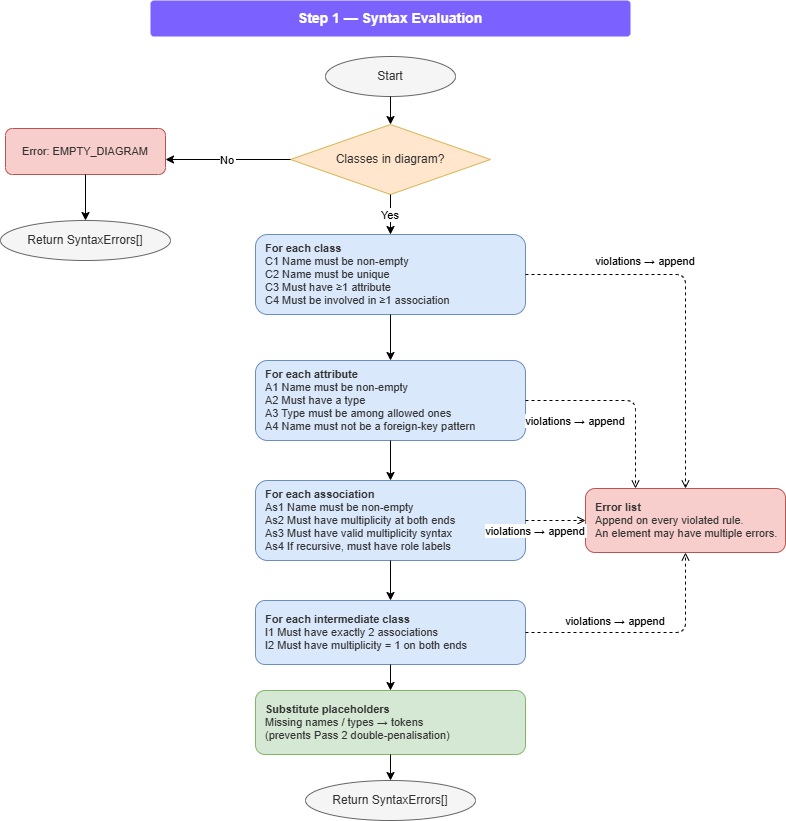
\includegraphics[width=0.75\linewidth]{syn_alg.png}
    \caption{Syntax evaluation algorithm}
    \label{fig:syn_alg}
\end{figure}

The semantic evaluation compares the student diagram against the reference solution, first looking for matches between reference elements and diagram elements according to their names: this is done by computing the \textit{normalized Levenshtein distance} between the diagram element's name and each reference element of the same type and its synonyms. A match is found if the distance between a diagram element's name and a reference name (or one synonym) is at most $0.25$, with the threshold being defined as such to tolerate writing errors and grammar mistakes. Elements that were found to have no name in the first step and thus received a placeholder name are not considered for evaluation in this step, to avoid assigning multiple errors to the same element.
After matches are found, subsequent assessments are performed on the matched elements to ensure domain details are also covered (e.g., attribute types, multiplicity values, association names), ensuring complete guidance for students; Figure \ref{fig:sem_alg} shows the steps that compose the algorithm for semantic evaluation.

\begin{figure}[ht]
    \centering
    
\includegraphics[width=0.75\linewidth]{sem_alg.png}
    \caption{Semantic evaluation algorithm}
    \label{fig:sem_alg}
\end{figure}

Lastly, the third step is used to identify minor modeling mistakes whose gravity is not high enough to consider them errors, but still count as design choices that can be improved; these mistakes are defined according to the pragmatic quality rules defined by Bolloju and Leung \cite{bolloju2006assisting}, and are reported to highlight issues that should be addressed but do not impact the completeness of the diagram. Figure \ref{fig:prag_alg} summarizes the pragmatic evaluation procedure applied at the end of each diagram check.

\begin{figure}[ht]
    \centering
    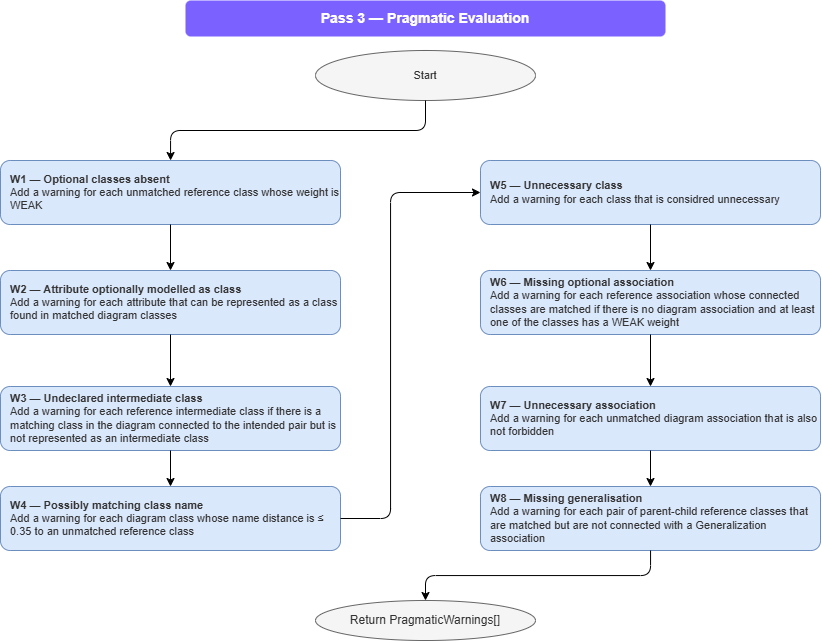
\includegraphics[width=0.75\linewidth]{prag_alg.png}
    \caption{Pragmatic evaluation algorithm}
    \label{fig:prag_alg}
\end{figure}


\section{Empirical Experiment with the Tool}

The development of UMLegend according to the new gamification framework was finalized in Autumn 2023, making it necessary to conduct a study to evaluate its effectiveness. Following the lessons learned from the BIPMIN experiment, it was decided to employ the tool in a single session first, to assess the effectiveness of the game mechanics on motivating the students and the tool's impact on learning performance, as well as to gather feedback before using the tool for the duration of a course. The experiment was conducted in January 2024 and followed a similar design to the one performed for evaluating BIPMIN: as such, the Goal-Question-Metric (GQM) template was adopted once again, expressing the purpose of the study as \textit{assess the impact of gamification on the production of UML class diagrams and their correctness from the point of view of Software Engineering teachers in the context of university courses}, with Table \ref{tab:gqm4} summarizing the experiment according to the template.


\begin{table}[ht]
  \rowcolors{2}{gray!25}{white}
\centering
\caption{GQM template for the experiment}
\label{tab:gqm4}
\small
\begin{tabular}{@{}p{0.3\columnwidth} p{0.55\columnwidth}@{}}
\toprule
Object of Study & Learning of UML Modeling \\
Purpose & Compare the traditional and gamified approach \\
Focus & Productivity, Correctness, Student Reception  \\
Context & Modeling tools \\
Perspective & Software engineering teachers \\
\bottomrule
\end{tabular}
\end{table}

\subsection{Study Design and Participants}

In the same vein as the 2023 experiment, participants were selected through convenience sampling among the students enrolled in the course \textit{Sistemi Informativi Aziendali}, offered as part of the Masters' Degree in Management Engineering, during the 2023-2024 academic year; participation was rewarded with 2 additional points on the exam grade, with assurance that participation was optional and that there would have been no consequences for not participating, or for participating in a suboptimal way. A total of 280 students took part in the study, split into 117 female students and 163 male students.

Contrary to the study performed in 2023, the experiment was conducted completely in presence at the end of the course, ensuring students had a sufficient level of modeling skill to perform adequately in the tasks; the UMLegend tool was served as a web application that students could access with their personal devices for the duration of the study.

Another similarity with the 2023 study was in the design of the experiment itself: the goal was to evaluate the differences between gamified and non-gamified UML class diagram modeling, and thus the within-subjects design was selected again. To allow for this comparison, a modified version of UMLegend was used for the study: while the long-term mechanics were kept in place for the entire study, the ability to mark exercises as non-gamified was added to the tool, and exercises marked as such offered no in-exercise mechanics and a less detailed feedback (e.g., a generic message stating that some classes were missing would be used rather than a separate message for each missing class).

The design was then set up to have students perform two exercises as tasks, solving one with the regular version and one with the non-gamified environment: the same 2x2 full factorial crossover design adopted for the original experiment was used in this scenario as well, keeping in mind the order of exercise and treatment as another variable and resulting in four possible combinations, which are presented in Table \ref{tab:exp_design}. Group assignment was random, resulting in four groups of 70 students.

\begin{table}[t]
  \rowcolors{2}{gray!25}{white}
\centering
\caption{Experiment Design for the 2024 UMLegend study}
\label{tab:exp_design}
\footnotesize
\begin{tabular}{@{}p{0.13\columnwidth} p{0.2\columnwidth} p{0.12\columnwidth} p{0.2\columnwidth} p{0.12\columnwidth}@{}}
\toprule
& \multicolumn{2}{c}{Task 1} & \multicolumn{2}{c}{Task 2} \\
& Exercise & Tool & Exercise & Tool \\
\midrule
Group 1 & Exercise 1 & Vanilla & Exercise 2 & Gamified \\
Group 2 & Exercise 1 & Gamified & Exercise 2 & Vanilla \\
Group 3 & Exercise 2 & Vanilla & Exercise 1 & Gamified \\
Group 4 & Exercise 2 & Gamified & Exercise 1 & Vanilla \\
\bottomrule
\end{tabular}%
\end{table}

The two exercises were selected among the ones offered as part of course exams held in past years and consisted of textual descriptions of real-life scenarios where a software application was to be implemented, requiring the design of a class diagram to support development. The exercises were estimated to have an average level of difficulty, ensuring that students close to the end of the course had a sufficient level of preparation to solve each of them in the allocated time window of 45 minutes.

After completing the two tasks, participants were asked to answer a questionnaire to measure their perception of the experience and of the game mechanics, as well as to gather opinions and feedback for improving the application.


\subsection{Research Questions and Metrics}

The following research questions were formulated to guide the experiment design:
\begin{itemize}
    \item \textbf{RQ1:} Does gamification improve the students' \textit{Productivity} in modeling UML class diagrams compared to non-gamified UML modeling?\\
    \emph{The reasoning behind this question is that gamification could provide a more engaging environment, leading students to make more changes in their diagrams and have them evaluated more frequently.}\\
    This question is further refined into:
    \begin{itemize}
        \item \textbf{RQ1.1:} Does the application of gamification impact the \textit{Size} of the diagrams made by the students?
        \item \textbf{RQ1.2:} Does the application of gamification impact the \textit{Attempts} made by students?
    \end{itemize}
    \item \textbf{RQ2:} Does gamification improve the \textit{Correctness} of the diagrams modeled by the students compared to non-gamified UML modeling?\\
    \emph{It is assumed that gamification could improve student performance by increasing diagram completeness and reducing the errors made by the students.}\\
    This question is further refined into:
    \begin{itemize}
        \item \textbf{RQ2.1:} Does the application of gamification impact the \textit{Completeness} of the diagrams produced by the students?
        \item \textbf{RQ2.2:} Does the application of gamification impact the \textit{Errors} found in the diagrams produced by the students?
    \end{itemize}
    \item \textbf{RQ3:} What is the students' \textit{Perception} of gamified UML modeling?\\
    \emph{The rationale behind this question is that gamification is positively perceived by the students with more involvement and willingness to adopt it.}\\
    This question is further refined into:
    \begin{itemize}
        \item \textbf{RQ3.1:} What is the perceived usability of the gamified UML modeling tool?
        \item \textbf{RQ3.2:} What is the appreciation of the gamified characteristics and mechanics in the gamified UML modeling tool?
        \item \textbf{RQ3.3:} What are the issues and improvement areas for the gamified UML modeling tool?
    \end{itemize}
\end{itemize}

Due to the experiment design remaining unchanged from the 2023 experiment, independent variables observed for analysis in the new study remained the same: the \textit{Treatment}, that is, the use of the gamified or non-gamified modeler, remained the main independent variable under scrutiny, while other independent variables considered as possible confounding factors were the \textit{Exercise} used as task and the \textit{Group} to which participants were assigned.

Independent variables were considered for research questions RQ1 and RQ2, since they dealt with data that could be analyzed with statistical methods, while metrics related to RQ3 were connected with the final questionnaire, and were analyzed with a qualitative approach. The collection of dependent variables was performed automatically with the tool: each evaluation launched by a students would record the current diagram and the state of game mechanics, with both the regular version and the non-gamified one. 

To answer RQ1, two dependent variables were considered: first, the \textit{Size} of submitted diagrams, computed as the count of classes, attributes, and associations, was recorded, with the assumption that adopting gamification would lead to significant changes in the number of elements present in a student's diagram, with the size of the reference solution adopted for the study as the target value. The second variable considered was the number of \textit{Attempts}, that is, the number of evaluations launched by a student during each task; this metric was collected for both the Vanilla and Gamified version, and was measured with the assumption that using gamification would lead students to perform more evaluations for their exercises. In the Vanilla version, changes in the obtainable experience points and in the diagram completeness score, as well as the count of errors, are still computed internally and stored despite not being shown to students.


The dependent variables selected to answer RQ2 were split according to the refined sub-questions: for RQ2.1, the \textit{Completeness} of diagrams was considered, with the reason being that adopting gamification would guide students to make significant improvement, and thus increase this metric; for RQ2.2, instead, three metrics were computed as the count of syntactic and semantic errors, as well as pragmatic warnings obtained with the final submitted diagram, with the assumption that gamification would have a positive effect and lead to a decrease in such counts.

The final questionnaire consisted of multiple sets of questions, with each set being focused around a specific sub-question. To answer RQ3.1, which aimed at assessing the overall student perception of the gamified experience, questions taken from the Technology Acceptance Model (TAM) \cite{lee2003technology} and GAMEX \cite{eppmann2018gameful} questionnaires were used. The GAMEX questionnaire was used in the same fashion as in the first BIPMIN study, to measure the six different aspects that characterize a gamified experience, while the TAM questionnaire was adopted to assess the overall student perception of the tool, measuring four high-level constructs such as Perceived Usefulness (PU, the belief that using an application would improve performance), Perceived Ease of Use (PE, the belief that using an application requires little physical and mental effort), Behavioral Intention to Use (BI, the measure of how much one would be inclined to use an application in a specific way), and Attitude Towards Usage (ATU, the measure of how much one would want to use an application). Answers to both questionnaires were expressed through a Likert scale going from a score of 1 (Strongly Disagree) to 5 (Strongly Agree).

To answer RQ3.2, a specific set of questions was created, centered around each of the implemented game mechanics: the same five questions were repeated for each mechanic, assessing the students' opinions about its perceived usefulness, influence in using the application, satisfaction, motivating effect, and distracting effect. Answers to these questions were expressed with the same Likert scale format used for the TAM and GAMEX.

Lastly, two open questions were included to answer RQ3.3, which students could use to report issues encountered during the study and to leave suggestions for improving the tool. 

%The data is available as an online resource\footnote{\url{https://doi.org/10.6084/m9.figshare.25968082.v2}}. 

\subsection{Analysis Method}
To answer the sub-questions derived from RQ1 and RQ2, the following null hypotheses were formulated:
\begin{itemize}
    \item \emph{${H_{s_{0}}}$:} The application of gamification has no statistically significant impact on the size of the diagrams produced by the students
    \item \emph{${H_{as_{0}}}$:} The application of gamification has no statistically significant impact on the number of attempts (diagram evaluations) made by the students
    \item \emph{${H_{pr_{0}}}$:} The application of gamification has no statistically significant impact on the completeness of the diagrams produced by the students
    \item \emph{${H_{syn_{0}}}$:} The application of gamification has no statistically significant impact on the number of syntax errors made by students
    \item \emph{${H_{sem_{0}}}$:} The application of gamification has no statistically significant impact on the number of semantic errors made by students
    \item \emph{${H_{prag_{0}}}$:} The application of gamification has no statistically significant impact on the number of pragmatic warnings raised by students
\end{itemize}

Assuming that the variables would not follow a normal distribution, it was decided to test these hypotheses using a non-parametric approach; the statistical method adopted was, according to the standard practice for conducting full factorial crossover experiments \cite{vegas2016crossover}, a repeated measures linear mixed model (ANOVA), comparing each metric separately depending on the the treatment, with the exercise and the group assignment being considered confounding factors that could threaten the validity of the results.

Furthermore, the significance level was adjusted with the application of Bonferroni correction to account for multiple comparisons and to counteract the risk of multiple statistical tests increasing the change of false positives; given a total of six statistical tests being conducted in the analysis, the p-value threshold was adjusted, with $\alpha_C = \alpha / n =  0.0083$ being needed to imply statistical significance. 


Lastly, RQ3 was evaluated with a questionnaire whose answers could not be analyzed with statistical hypothesis testing; as a consequence, descriptive statistics were used to answer RQ3.1 and RQ3.2. The approach used was to compute, for each group of questions related to the same topic (e.g., Perceived Usefulness for the TAM, Enjoyment for the GAMEX, or a given game mechanic) the average score, rounded down, given by each student as the representation of said student's opinion. The distribution of opinions was then reported with stacked diverging bar charts, to rank each questionnaire's constructs and measure the overall perception.

RQ3.3, instead, was analyzed using open-ended questions and, as such, a similar procedure as the one used for the BIPMIN study was performed, adopting the \textit{open coding} approach defined by the Straussian Grounded Theory approach.

The goal of the analysis was to identify topics in the students' answers and then to group answers to identify common topics and opinions; the coding process involved the analysis of each answer one by one to identify the most compatible topic among the existing one, tagging the question with the topic if one was found, or creating a new, suitable one otherwise, resulting in the creation of the topic set. After all answers had been analyzed once, they were all reviewed a second time to ensure the original topic was still suitable or if there was another, more relevant one to tag the answer with; following that, a final review was performed to locate answers that fit more than one topic, resulting in certain answers having more than one relevant topic.

\subsection{Results}

The summary statistics for RQ1-related metrics, that is, the size of the final saved diagram and the number of checks performed for each exercise, are reported in in Table \ref{tab:rq1_4}. These statistics (minimum, maximum, mean, median, standard deviations) have been computed separately depending on the treatment, and Figure \ref{fig:rq1_4} shows a combined box and violin plot that represents their distribution.

\begin{table}[htbp]
  \rowcolors{2}{gray!25}{white}
    \small
    \centering
    \caption{Maximum, Minimum, Average, and Median scores for \textit{Productivity} metrics}
    \begin{tabular}{lrrrr}
    \toprule
    & Min & Max & Mean (SD) & Median \\
    \midrule
    Size (V)& 9 & 64 & 34.61 (9.09) & 33 \\
    Size (G) & 3 & 69 & 34.18 (9.40) & 32 \\
    Attempts (V) & 0 & 35 & 5.68 (5.00) & 3 \\
    Attempts (G) & 1 & 43 & 6.66 (7.16) & 4 \\
    \bottomrule
    \end{tabular}
    \label{tab:rq1_4}
\end{table}


\begin{figure}[H]
    \centering
    \begin{subfigure}{0.7\linewidth}
        \centering
        
\includegraphics[width=\linewidth]{Template_Latex_ScuDo_Tesi/Chapter4/size_violin.png}
        \caption{Box and violin plot for the \textit{Size} metric}
        \label{fig:rq1_size}
    \end{subfigure}\hfill
    \begin{subfigure}{0.7\linewidth}
        \centering
        
\includegraphics[width=\linewidth]{Template_Latex_ScuDo_Tesi/Chapter4/attempts_violin.png}
        \caption{Box and violin plot for the \textit{Attempts} metric}
        \label{fig:rq1_attempts}
    \end{subfigure}
    \caption{Box and violin plots for RQ1 metrics}
    \label{fig:rq1_4}
\end{figure}

For what concerns \textit{Size}, the plot shows that the distribution is more or less equal, with the mean value being slightly higher for the non-gamified version, implying that students produce less dense diagrams when using gamification. \textit{Attempts} achieved a different result, with a higher number of checks being performed on average with the gamified version, and overall higher numbers compared to the Vanilla version. A possible implication is that gamification does may not lead students to make significant changes, but it could be a guiding factor in performing more automated assessments.

An ANOVA test was performed on the two Productivity metrics and their distribution to answer RQ1 and possibly reject the two null hypotheses, with the goal of identifying a statistically significant impact of gamification on student productivity; Table \ref{tab:rq1_4_anova} presents, for each metric and the corresponding hypothesis, the results of the ANOVA test according to the main factor (gamification against no gamification) and the two confounding factors (exercise and the combination of treatment and exercise).


\begin{table}[ht]
  \rowcolors{2}{gray!25}{white}
\footnotesize
\centering
\begin{tabular}{lcccc}
    \toprule
         Factor / vars:& 
         \multicolumn{2}{c}{Size (${H_{s_{0}}}$)} & \multicolumn{2}{c}{Attempts (${H_{as_{0}}}$)} \\
         & coeff. & p-value & coeff. & p-value \\
    \midrule
    Treatment & -0.436 & 0.577 & 1.589 & \textbf{2.45e-03} \\
    Exercise & -8.3429 & \textbf{$\lt$ 2e-16} & 0.2964 & 0.574 \\
    Group & 0.1614 & 0.644 & -0.3107 & 0.187 \\
    \bottomrule
    \end{tabular}
\caption{Results of the statistical analysis for RQ1 metrics: Size and Attempts. Statistically significant p-values are in bold ($\alpha = 0.0083$)}
\label{tab:rq1_4_anova}
\end{table}


The analysis considers the non-gamified version as the reference one, confirming what was highlighted by Figure \ref{fig:rq1_4}: gamification leads to slightly smaller diagrams but a higher number of evaluations, encouraging students to interact more and more with the game mechanics.

The p-value associated with \textit{Size} is not statistically significant and, consequently, the null hypothesis ${H_{s_{0}}}$ cannot be rejected: gamification does not impact the size of student-made diagrams in any way, and as a consequence does not lead students to make significant changes.

Conversely, the p-value obtained by comparing the average number of \textit{Attempts} is statistically significant, implying that gamification does have an impact on the metric: with the average number of submissions being higher with the gamified version it is possible to reject hypothesis ${H_{as_{0}}}$ and affirm that gamification has a positive effect on the students' tendance to automatically evaluate diagram and, as a consequence, on their overall commitment.

For what concerns confounding factors, the only statistically significant result is that \textit{Size} depends on the exercise: the analysis took the first exercise as reference, and the negative value of the coefficient implies that the second exercise had a much lower size on average (30.23 against 38.57); as a point of comparison, the reference solution for the two exercises had a total size of 43 elements and 32 elements respectively. The difference in average sizes obtained by the students is in line with the fact that the two exercises also require different elements to be considered correct; however, this difference could also imply that one exercise required more effort to fully represent the intended domain and, consequently, be more complex than the other.


\answer{RQ1}{Applying gamification to class diagram exercises had no impact on the diagram size, implying that it does not encourage students to make significant changes to their diagrams but, possibly, to edit the existing elements to make them fit the context. The statistically significant increase on the number of attempts, instead, can be seen as a positive effect of gamification, since it means that tying the evaluation to the game mechanics makes students more inclined to evaluate their solution, making it reasonable to assume a positive effect on student commitment. Productivity metrics were relatively not impacted by other factors involved in the study design, with the only significant effect being on diagram size depending on the exercise: with one exercise having a lower element count, on average, it may be possible that one exercise was easier, impacting the validity of the study.}

To answer RQ2, diagram completeness and the count of errors (syntactic, semantic, and pragmatic warnings) were collected through the tool; Table \ref{tab:rq2_4} lists the minimum, maximum, mean, median, and standard deviation for these four metrics depending on the two treatment, while Figure  shows the combined box and violin plots for the distribution of the four metrics, also according on the use of gamification or not.

\begin{table}[htbp]
  \rowcolors{2}{gray!25}{white}
    \footnotesize
    \centering
    \caption{Maximum, Minimum, Average, and Median scores for correctness metrics}
    \begin{tabular}{lrrrr}
    \toprule
    & Min & Max & Mean (SD) & Median \\
    \midrule
    Completeness (V) & 0 & 98 & 42.54 (13.09) & 44  \\
    Completeness (G) & 9 & 95 & 47.21 (13.18) & 46 \\
    Syntax Errors (V) & 0 & 31 & 5.4 (6.48) & 3 \\
    Syntax Errors (G) & 0 & 32 & 3.79 (5.51) & 1 \\
    Semantic Errors (V) & 2 & 18 & 9.64 (2.91) & 9 \\
    Semantic Errors (G) & 2 & 18 & 8.71 (2.69) & 8 \\
    Pragmatic Warnings (V) & 0 & 8 & 2.05 (1.54) & 2 \\
    Pragmatic Warnings (G) & 0 & 10 & 2.20 (1.61) & 2 \\
    \bottomrule
    \end{tabular}
    \label{tab:rq2_4}
\end{table}

\begin{figure}[H]
    \centering
    \begin{subfigure}{0.5\linewidth}
        \centering
        
\includegraphics[width=\linewidth]{Template_Latex_ScuDo_Tesi/Chapter4/compl_violin.png}
        \caption{Box and violin plot for the \textit{Completeness} metric}
        \label{fig:rq2_compl}
    \end{subfigure}\hfill
    \begin{subfigure}{0.5\linewidth}
        \centering
        
\includegraphics[width=\linewidth]{Template_Latex_ScuDo_Tesi/Chapter4/syn_violin.png}
        \caption{Box and violin plot for the \textit{Syntax Errors} metric}
        \label{fig:rq2_syn}
    \end{subfigure}\hfill
    \begin{subfigure}{0.5\linewidth}
        \centering
        
\includegraphics[width=\linewidth]{Template_Latex_ScuDo_Tesi/Chapter4/sem_violin.png}
        \caption{Box and violin plot for the \textit{Semantic Errors} metric}
        \label{fig:rq2_sem}
    \end{subfigure}\hfill
    \begin{subfigure}{0.5\linewidth}
        \centering
        
\includegraphics[width=\linewidth]{Template_Latex_ScuDo_Tesi/Chapter4/prag_violin.png}
        \caption{Box and violin plot for the \textit{Pragmatic Warnings} metric}
        \label{fig:rq2_prag}
    \end{subfigure}
    \caption{Box and violin plots for RQ2 metrics}
    \label{fig:rq2_4}
\end{figure}

Overall, the distribution of metrics paints an encouraging picture for what concerns the effect of gamification: diagram completeness is on average higher, and both syntactic and semantic errors are lower as well; it can be assumed that gamification can lead to better student performance, with more correct elements being represented and fewer errors being made. Pragmatic warnings, however, are higher on average when gamification is applied: a possible interpretation could be that, since they are presented as minor issues that do not impact correctness and can simply be represented in a better way, students may have decided to ignore them.

To identify whether the treatment or other design factors could have impacted the correctness metrics an ANOVA test was performed; Table \ref{tab:rq2_4_anova} summarizes the result of this analysis by showing the resulting difference coefficient and corresponding p-value for each of the four metrics and associated null hypothesis for treatment, exercise, and group assignment.

\begin{table}[ht]
  \rowcolors{2}{gray!25}{white}
\footnotesize
\centering
\begin{tabular}{lcccccccc}
    \toprule
    Factor / vars: &
    \multicolumn{2}{c}{${H_{pr_{0}}}$} &
    \multicolumn{2}{c}{${H_{syn_{0}}}$} &
    \multicolumn{2}{c}{${H_{sem_{0}}}$} &
    \multicolumn{2}{c}{${H_{prag_{0}}}$} \\
    & coeff. & p-value & coeff. & p-value & coeff. & p-value & coeff. & p-value \\
    \midrule
    Treatment & 4.6750 & \textbf{2.96e-05} & -1.6107 & \textbf{1.62e-03} & -0.9286 & \textbf{9.80e-05} & 0.1500 & 0.259 \\
    Exercise  & 10.1893 & \textbf{$<$ 2e-16} & -2.3821 & \textbf{2.76e-06} & -3.4143 & \textbf{$<$ 2e-16} & -0.80714 & \textbf{6.82e-10} \\
    Group     & -0.8407 & 0.095 & -0.2993 & 0.192 & -0.0900 & 0.402 & 0.0300 & 0.614 \\
    \bottomrule
\end{tabular}
\caption{Results of the statistical analysis for RQ2 metrics. Statistically significant p-values are in bold ($\alpha = 0.0083$)}
\label{tab:rq2_4_anova}
\end{table}

The ANOVA test shows that, when accounting for the treatment, gamification leads to higher completeness on average with a statistically significant p-value: as a consequence, the null hypothesis ${H_{pr_{0}}}$ can be rejected, and it can be said that gamification leads to more correct diagrams. Similarly encouraging results can be observed for syntax and semantic errors: both metrics yield a lower average count for the gamified version and their corresponding ANOVA tests both obtained a statistically significant p-value, implying that using gamification leads to less errors, on average. Null hypotheses ${H_{syn_{0}}}$ and ${H_{sem_{0}}}$ can both be rejected: gamification has a positive effect on student performance by reducing both syntax and semantic errors, meaning that it could be useful for learning both modeling rules and domain adherence. The non statistically significant p-value for pragmatic warnings means that it is not possible to reject ${H_{prag_{0}}}$.


The analysis focused around confounding factors showed that, when considering the exercise as reference, all four metrics have statistically significant differences, with the second exercise showing a higher average completeness (around 10\% more) and lower counts for both syntax and semantic error and pragmatic warnings, reinforcing the assumption that the second exercise was easier than the first. While this may have an impact on the overall results, the experiment's design counterbalances the exercise's impact, thanks to having students perform different exercises in different order and with different treatments. The positive effect of the design can also be seen by the p-values obtained when analyzing the values according to the order of tasks and treatments: with no statistically significant differences, it can be said that no learning effects were in place.

\answer{RQ2}{Gamification had a positive effect on the overall diagram correctness, leading to an increase in completeness as well as a reduction in both syntax and semantic errors, resulting in more correct diagrams. It can be said that the various features helped students understand what they needed to represent and which specific details had to be corrected. The two exercises selected as tasks had different results as well, with one appearing to be easier than the other, with a statistically significant difference in both completeness (higher on average) and all three error types (lower on average); the potential impact of this discrepancy was however mitigated by the experiment design.}

To answer RQ3 and its sub-questions, a questionnaire divided into multiple parts was given to students at the end of the study. The part related to RQ3.1 dealt with the general usability of the tool as well as the perception of the gamified experience with questions taken from the TAM and GAMEX questionnaires; the distribution of the students' opinions, computed as the average score for each construct of both questionnaires, are shown in Figures \ref{fig:rq3_4_tam} and \ref{fig:rq3_4_gamex}.

\begin{figure}[H]
    \centering
    \begin{subfigure}{0.5\linewidth}
        \centering
        
\includegraphics[width=\linewidth]{Template_Latex_ScuDo_Tesi/Chapter4/tam.png}
        \caption{Distribution of answers to the TAM questionnaire}
        \label{fig:rq3_4_tam}
    \end{subfigure}\hfill
    \begin{subfigure}{0.5\linewidth}
        \centering
        
\includegraphics[width=\linewidth]{Template_Latex_ScuDo_Tesi/Chapter4/gamex.png}
        \caption{Distribution of answers to the GAMEX questionnaire}
        \label{fig:rq3_4_gamex}
    \end{subfigure}
    \caption{Distribution of students' average opinions for RQ3.1 constructs}
    \label{fig:rq3_4}
\end{figure}

Regarding answers to the TAM questionnaire, opinions appear to be quite positive, given that at least half of the participants have a positive average opinion (equivalent to answering \textit{Agree} to the entire construct) for each of the four constructs; the distribution of answers given for Attitude towards Usage (72\% Agree + Strongly Agree) and Perceived Ease of Use (65\% Agree + Strongly Agree) are particularly encouraging, since it means that students felt that using UMLegend was something easy to learn, and that it was also a tool students would feel inclined to use more. Negative opinions being quite rare is also a positive result: Perceived Usefulness was the construct with the highest total (13\% Disagree + Strongly Disagree), making it the less successful TAM construct. A possible interpretation could be that the tool appears easy and interesting to use but may not seem as impactful for learning, perhaps as a consequence of using it at the end of a course rather than over time.

Answers given to the GAMEX questions, however, are more on the neutral side, with two thirds of the constructs having a distribution of positive opinions lower than 20\%, with many of them also having at least 30\% total negative opinions. The only clearly positive results obtained with the GAMEX questions concern the Enjoyment construct, with a total of 49\% positive opinions, and the Possible Negative Effects one, with 79\% disagreeing opinions. It can be assumed that UMLegend is perceived as a fun and engaging tool to support modeling activities with very little negative impact such as frustration or hostile design choices.

Unfortunately, since the remaining for constructs tend to have distributions of opinions between neutral and negative, certain limits of the tool emerge: creative thinking is not entirely supported despite the freedom given for modeling choices, and the tool does not feel particularly stimulating and immersive. It is possible that these results depend on the single-session design of the experiment, and that continuous adoption may improve the tool's perception in these aspects.

\answer{RQ3.1}{The UMLegend tool was favorably received by students in terms of its general usability, as highlighted by the answers given to the TAM questionnaire: students felt that the tool was easy to use, and stated they would be inclined to use it for modeling tasks; however, questions related to the perceived usefulness ranked the lowest among all four constructs, meaning that the educational benefits may need to be conveyed more clearly. The gamification-specific perception of the tool, conversely, was not as positive: while most students agreed that using the tool is an engaging and fun experience that does not feel frustrating or makes the player feel antagonized, certain aspects such as the immersiveness or the support for creativity and freedom still feel limited, implying the need for a redesign of certain mechanics.}

The second block of the questionnaire, designed to answer sub-question RQ3.2, included custom made questions repeated for each of the game mechanics that investigated whether students perceived the mechanic as useful, if the mechanic influenced their use of the tool, if students were satisfied with how they interacted with the mechanic, if they felt motivated by it, and if it was perceived as distracting. For each student, the overall opinion was computed similar to how it was done for the TAM and GAMEX questionnaires, given that the answer format was the same (Likert scale values ranging from 1 to 5), although with one difference: since the fifth question had a negative connotation, the average was computed using its opposite value (e.g., a \textit{Strongly Disagree} answer was considered a \textit{Strongly Agree} when computing the value) to offset the negative value. The average answer was computed for each game mechanic, to identify the most appreciated ones; Figure \ref{fig:rq32_4} shows the overall distribution of opinions.

\begin{figure}[htpb]
    \centering
    
\includegraphics[width=\columnwidth]{Template_Latex_ScuDo_Tesi/Chapter4/mechs.png}
    \caption{Distribution of answers related to the different game mechanics}
    \label{fig:rq32_4}
\end{figure}

Overall, it can be said that all game mechanics have been somewhat well received, with all of them having a positive average opinion of least 33\%. Moreover, the distribution seems to confirm the same perception of game mechanics that was found with the BIPMIN study: game mechanics that provide direct assistance in solving an exercise are the most appreciated, given that for Error Lists, Indicators, and Diagram Feedback at least half of the participants had positive opinions and less than 10\% had negative ones. Mechanics that were conceived for long-term usage such as Leaderboards and Avatar Customization were also well-received, supporting their inclusion in the new framework and reinforcing the necessity for a longitudinal study on gamified modeling education. However, the fact that Avatar Customization was the mechanic with the highest percentage of negative opinions (27\%) may not only depend on the single-session design and on the need to unlock additional props but also on the perception itself, which may appear childish and negatively impact the overall tool perception.

\answer{RQ3.2}{All game mechanics have been appreciated by at least a third of the participants, suggesting that the redesign was successful and encouraging future and continuous use of UMLegend. The detailed distribution of opinions confirms what was discovered with the first empirical study: mechanics that provide direct assistance for completing exercises by specifying what needs to be improved and how are the most appreciated, and mechanics intended for long-term usage rank slightly lower.}

Lastly, the final block of the questionnaire consisted of two open-ended questions, one asking for issues encountered when using the tool and another asking for suggestions and possible improvement areas. After performing an open-coding analysis on the answers given by students, a total of 6 topics were found for the first question, after excluding 227 answers that reported no issue; similarly, 142 answers to the second question were either empty or had no suggestion and were not considered for the analysis. The topics found in the two questions can be seen in Figures \ref{fig:rq3_4_issues} and \ref{fig:rq3_4_issues}.

\begin{figure}[H]
    \centering
    \begin{subfigure}{0.5\linewidth}
        \centering
        
\includegraphics[width=\linewidth]{Template_Latex_ScuDo_Tesi/Chapter4/issues.png}
        \caption{Topics found in the open-ended question asking for issues encountered during the study}
        \label{fig:rq3_4_issues}
    \end{subfigure}\hfill
    \begin{subfigure}{0.5\linewidth}
        \centering
        
\includegraphics[width=\linewidth]{Template_Latex_ScuDo_Tesi/Chapter4/improv.png}
        \caption{Topics found in the open-ended question asking for suggestions for improving UMLegend}
        \label{fig:rq3_4_impr}
    \end{subfigure}
    \caption{Results of the open coding procedure on the answers given to the two open-ended questions}
    \label{fig:rq33_4}
\end{figure}

Regarding issues, the most common topic related to issues in setting up the tool and using its features, something that depends on the explanations given at the beginning of the study, that may have been unclear or limited; more relevant issues cover problems in the modeler implementation and the feedback, which was judged limited and unclear. The modeler issues may depend on the fact that students were used to a different modeling tool (Signavio Academic), with more features compared to the Apollon modeling library used in the tool such as an easier way to specify attributes or better association handling, a part of the modeling interface that was considered complex and unfriendly.

These two topics found in issues were also found in the answers given to the question asking for suggestions: an improved and friendlier modeler, closer to the one students were used, was the most common request, indicating that perhaps the neutral perception of the tool depended not only on the game mechanics but on the modeling aspect as well. The feedback mechanisms were also mentioned by several answers as something that could be improved by explaining errors more in detail or by also highlighting correct elements.

Other common suggestions mentioned reworking the user interface by changing the way an exercise's text is displayed or letting students select text from the description and create classes starting from the text; certain comments also stated the need to make the evaluation engine more flexible, since there were scenarios in which certain synonyms were not considered valid despite being correct due to not appearing in the reference solution. Experience management was also mentioned as a part of the system to revise, since students stated they did not feel that correcting errors actually helped increase the experience reward again, and errors reducing the value felt more impactful; suggestions to address this issue mentioned either reducing the penalty caused by erorrs or having errors reduce experience only on their first appearance.

Lastly, rarer suggestions covered once more findings from the original BIPMIN study related to the single-session design: leaderboards and levels were not considered impactful, with some students suggesting their removal, tutorials were also mentioned as a potentially relevant feature, and some students explicitly stated they would have preferred using the tool more if it was available for a longer period of time.

\answer{RQ3.3}{The analysis of the students' open comments helped identify certain limitations of UMLegend such as the somewhat unfriendly modeling interface, the need to expand feedback to be more detailed, potential improvements to the user interface, and a rework of the experience management to make it more friendly and less penalizing. The evaluation engine was still a point of concern due to issues with certain synonyms and modeling choices not being considered in advance for the reference solution, but was a less severe problem in comparison with the 2023 study.}

\subsection{Threats to validity}

Following the characterization by Wohlin et al. \cite{wohlin2012experimentation}, the threats to the validity of the empirical study are discussed below.

\textbf{Threats to internal validity:} the crossover design could have introduced learning effects, due to having students perform two tasks consecutively and using tools with a common base; it may also be possible that the second task may have been influenced by the first one. The different difficulty level of the two exercises, which emerged during the analysis, may also have impacted the results. The choice to use a 2x2 factorial design mitigated these threats. 

Other relevant internal threats depend on the limited variability in the reference solution, since certain correct modeling choices may not have been recognized as such, potentially introducing a negative bias in the evaluation of the diagrams. The use of synonyms for each named elements and the support for small grammar mistakes and typos mitigated this threat.

Lastly, considering feedback a game mechanic may also have had an impact on the results: using a detailed feedback mechanism in the gamified version and a simplified, generic one for the non-gamified one may have reduced the scores for the latter version.

\textbf{Threats to External Validity:} it may not be possible to generalize the results to students with different modeling skill levels. For example, performing a similar study at the beginning of the course may yield different results, same performing it with students from a different background. Moreover, the benefits may apply specifically in an university setting and not in industrial modeling scenarios.


\textbf{Threats to Construct Validity:} the metrics observed to answer the research questions may not be the most suitable to represent the actual observed constructs. For example, productivity may have been measured with the time spent to complete each exercise, although such metric does not necessarily imply better performance, and correctness may have been measured with different rules and criteria, perhaps yielding different completeness scores and error counts.


\textbf{Threats to Conclusion Validity:} non-parametric statistical tests were used, and since all metrics were collected automatically by the tool the risk of human errors was minimized. There may have been a risk of confounding factors depending on the random allocation of participants to the four groups, resulting in certain groups having more capable participants, but this threat can be considered improbable with the assumption that participants all had a similar modeling skill level due to performing the study at the end of the course.

\subsection{Key findings and lessons learned}

The empirical study aimed to continue what was started with the 2023 study by investigating whether a gamified modeling tool, developed according to the lessons learned from the first study, could have a positive influence on student performance and be well received by a sample of the intended users for such a tool (university students of modeling courses). The results were more encouraging compared to the first study, and helped identify key issues to address in the latter part of the PhD course. 

A relevant result comes from the positive impact of gamification on the number of evaluated checks made by students: while this confirms a similar trend identified in the first empirical study, it also strengthens the conviction that modeling activities benefit from game mechanics being tied to automated diagram assessment and auto-evaluation, leading to an increase in student commitment.

Additionally, gamification also had a positive effect on diagram correctness, with both higher average completeness and lower average syntax and semantic error counts. This result is particularly encouraging when compared to the original study's result, where only semantic correctness was positively affected by gamification; moreover, the original interpretation of semantic correctness for the 2023 study could be considered equivalent to the overall diagram completeness, rather than the adherence itself to the intended domain. As a consequence, the UMLegend study confirmed the benefits of gamification on helping students represent correct diagrams, and also introduced the possibility of said strategy being useful for learning modeling rules. 

The revised implementation of game mechanics also led to an improvement in student perception: the post-study questionnaire showed that UMLegend is a fairly easy to use application, with potential for long-term use and possible benefits, while also being fun, engaging, and with little to no negative aspects such as frustration or hostility toward users, according to the students; certain gamification-specific aspects, however, were not all rated as highly, with limited freedom of action and creativity, as well as immersiveness, being causes of concern. These observations are also in line with the original study, and point to a limitation in the single-session experiment design: it may be reasonable to assume that longitudinal usage would increase aspects such as freedom and immersion.

The post-study questionnaire also confirmed the findings described in Chapter 3 related to game mechanics: students tend to appreciate the most mechanics such as diagram feedback or error lists that directly point out what are the errors in a diagram and provide explanations on how to correct them, while mechanics intended for longitudinal use such as levels and leaderboards, while still appreciated, were considered less impactful, with a few students even suggesting their removal from the tool. It can be deducted that single-session studies, while effective for understanding whether gamification can improve diagram completeness and student understanding of modeling rules, are not sufficient to properly assess the benefits and perception of gamified modeling education, and longitudinal studies are also necessary.

Lastly, while results are overall positive and encouraging, certain issues remain such as the unfriendly modeling canvas, which felt frustrating to use compared to the platform students were used to, the excessively strict experience system, which was considered too penalizing, although with less frequency compared to similar complaints recorded after the first study. The evaluation engine was also mentioned by students as a limit of the tool, despite the implementation allowing for more synonyms and variations in names, certain correct modeling choices were marked as incorrect; this was the most common issue in the original study, and it still appears to be a relevant problem to consider, although far less students mentioned it as such.

\articleSummary{
color1
}{
Summary of the empirical study
}{
The empirical experiment demonstrated that the new gamification framework can positively affect student commitment, diagram correctness and student understanding of modeling rules, with higher diagram completeness and fewer syntactic and semantic errors. The students' reception of the tool's usability was largely positive, while the gamified experience was perceived as enjoyable but not fully immersive, an expected limitation given the single-session nature of the study. The feedback mechanics were the most appreciated components of the tool, reinforcing the design priority given to immediate, actionable feedback in the framework. The main areas for improvement concern the modeling interface, whose perceived unfriendliness detracted from the overall experience, and the evaluation engine, which would benefit from greater flexibility in accepting alternative correct solutions.
}
\begin{comment}
    
\subsubsection{Limitations}
\label{sec:eval_limitations}

Two design limitations of the current evaluation engine are worth stating explicitly, as they directly informed the research directions outlined in Section~\ref{sec:future_work}.

\emph{Single reference solution.}  The engine compares the student diagram against exactly one canonical solution.  An alternative representation that a human evaluator would accept as correct—for example, modelling a concept as an intermediate class rather than as a plain association—may be flagged as an error if the reference does not include it.  Synonym lists mitigate this issue for naming variation but cannot address structural variation.

\emph{Synonym completeness.}  The quality of the semantic matching depends on the exhaustiveness of the synonym lists defined by the instructor.  A valid student label that was not anticipated during solution creation will be classified as non-matching, producing a false-negative.  The open-ended questionnaire responses collected in the experiment (Section~\ref{sec:results_rq3_3}) confirm that this limitation was noticeable to students: improving the modeller was the most frequently cited topic (38 answers), while a more flexible evaluation system was the fourth most common (approximately 20 answers).

Both limitations motivate the use of large language models as semantic similarity judges, an avenue that is explored as part of the future research programme described in Chapter~\ref{ch:future}.

\end{comment}
\chapter{The improved BIPMIN tool}
\label{ch5}

The development of the framework described in the previous chapter aimed at addressing the issues that had emerged with the empirical study with BIPMIN, leading to the development of a new tool and the execution of a second experiment with a similar design, to observe whether a new set of mechanics and a revised evaluation approach could make a gamified tool more effective. The framework was designed with the goal of supporting longitudinal use, implying the need of a specific evaluation procedure aimed at testing its potential benefits over a period of time beyond that of a single experiment. For this purpose, it was decided to redevelop the BIPMIN application, which had already proved the benefits of gamification applied to BPMN modeling, in accordance with the new selection of game mechanics, and to use this new version for the practical activities of the Information System course, where the original tool was tested.

The goal of this new study was to explore a different research direction: instead of comparing the gamified approach with regular modeling activities, the purpose was to observe whether continuous use of a gamified environment would lead to measurable improvements in the students' BPMN modeling knowledge and final performance. This chapter describes how the BIPMIN tool was redesigned according to the new framework and then presents the results of the study, focused on both the overall student perception of the gamified experience and on the empirical evaluation of how the tool impacted the students' grades and learning progression over time. The work described in this chapter has been split into two research articles: a first experience report focused on student perception and lessons learned was presented in \cite{garaccione2024ease}, while the empirical evaluation was described in \cite{garaccione2024esem}.

\section{Limitations of the existing version}

The original empirical study conducted in January 2023 identified a clear set of lessons and issues with the first implementation of the BIPMIN tool that guided the latter part of the PhD course's first year, leading to the implementation of UMLegend.

The first, and most significant, limitation was found in the rigid evaluation engine: despite the introduction of a semantic assessment check for assessing the content of a diagram (element names, types, position in relation to other elements) beyond regular adherence to syntax rules, the reference solution remained constrained to a single target model with limited variability in the set of accepted alternative ways to represent each process part. Many students who had produced a diagram semantically equivalent to the reference but with variations such as different element names, alternative structural choices or unexpected synonyms in part of the names got penalized by the evaluator not recognizing their work as correct, an assessment that would be found as such by a human observer. This resulted in continuous penalization that was in turn identified as the main source of dissatisfaction, resulting in the neutral perception of the overall experience highlighted by the answers to the GAMEX questionnaire; the key lesson found from this issue was that the game mechanics would not work as expected if they relied on an evaluation that students would perceive as unfair. 

Another limitation was connected to the results related to the impact of gamification over syntactic correctness: the original study showed a positive impact on semantic quality, highlighting that gamification could help students produce more correct models, but no similar effect could be observed regarding syntax quality and, consequently, on the benefits related to learning basic BPMN modeling rules. The reason for this result depends on the study's design: by conducting the experiment at the end of the course, students were already knowledgeable about BPMN syntax, especially because of the syntax enforcing feature present in the editor they were used to (Signavio Academic); this meant that students could be considered as experts on the syntactic point of view, highlighting the need to conduct a similar assessment earlier in the course, when students begin facing BPMN problems and need support and assistance to learn the key concepts, which is what gamification could help with and one of the goals of the PhD research.

Lastly, the implementation of the penalty mechanic, which was selected to introduce a negative motivator and discourage students from continuously submitting unchanged solutions, led to excessive frustration due to unexplained feedback behind the errors and consequent inability to understand why certain modeling choices were considered incorrect. 

Overall, the combination of a limited evaluation engine and excessively strict game mechanics led to the experience being seen in a neutral light, reducing the engaging effect of gamification, and the execution of the study at the end of the course limited the ability to assess its educational impact. 

\section{Tool changes according to the UMLegend framework}

After identifying the limitations with the original BIPMIN implementation, development of a new version started during Spring 2023 according to the gamified framework identified with the creation of UMLegend, making sure that both tools would share a common design logic adapted to the specific modeling domains, with the end goal of merging them in a single, multi-purpose educational environment. The development process led to the complete re-implementation of the evaluation engine as well, to extend the tool's ability to assess a diagram's correctness.

The same design choices made for UMLegend applied to the new version of BIPMIN: a separate client interface for teachers was implemented to support long-term course management, allowing for the creation of student profiles, new exercises, and most importantly reference solutions for each exercise, moving forward from the original implementation where solutions were hard-coded with no easy way to change them. On the student side, a homepage was added to allow for profile and avatar customization, as well as easy access to exercises. The implementation of game mechanics according to the UMLegend structure was guided by the new evaluation engine, which was identified as the first necessary change to improve the tool and make it suitable for long-term use.

\subsection{Evaluation Engine}

The behavior behind the new evaluation engine kept the same logic as the version used for the study: the evaluator would have to simulate the behavior of a teacher who looks at a diagram and identifies elements that represent specific parts of the target process and assesses errors such as wrong ordering of elements, elements belonging to different pools/lanes, and incorrect message exchanging.

The use of \textit{Process Parts} as the logical blocks to base a reference solution on remained as the key idea behind the evaluation engine; however, it became obvious after the study that each process part, and each element inside them, had to be assessed separately, with relationships between elements and parts being assessed at a later step in the evaluation, following identification of matching process parts. As a consequence, the data structure that implements reference solutions was restructured to distinguish between structural elements (pools, lanes, sub-processes), process parts, and forbidden elements.

\textit{Business Entities} were added as structures that were used to identify the pools expected to be included in a diagram. For each of them, a unique name was required, to express the corresponding pool both in feedback mechanics and in relationship to other elements in the solution; a set of synonyms could also be specified for each entity, allowing for more ways to express the same concept and leading to a match if a student's diagram included a pool with a name similar enough to either a synonym or the reference name. Furthermore, the ability to specify whether an entity was external pr not, requiring the use of a collapsed pool to represent it, was added, together with the ability to mark an entity as mandatory or as one that can be omitted without causing an error.

\textit{Actors} were used to represent the possible lanes that could be included in a diagram's pools. A unique reference name would identify each actor, with the list of possible synonyms being used as well, and, for each actor, the identifier of its parent pool An actor is considered represented correctly if there is a lane with a similar name to one of the allowed ones, if the parent business entity has a matching pool, and if the matching pool contains the matching lane; in case a matching pool is not found for a given business entity, all actors are automatically considered not found.

\textit{Sub-process} objects were used to identify the corresponding diagram elements that could group together multiple tasks and events inside a larger pool. Each object of this type could specify the parent element (either a pool or another sub-process) and whether it is a regular or an event-triggered sub-process, in which case it was also possible to state whether it could interrupt the parent element or not.

\textit{Forbidden Entities} were used to identify names that could not be used to represent pools or lanes, marking errors such as using names intended for business entities to represent actors (or vice-versa), including actors and entities that do not interact with the process, or representing the system or parts of it as an actor rather than as the entire diagram.

Lastly, the definition of \textit{Process Parts} was completely redone to allow for a more thorough and less strict evaluation: first of all, each part could be represented by multiple alternative groups of elements, where each element could be defined in different alternative ways to support the variability of correct representation. Each given element in a group would have a unique identifier in the solution and state the possible options such as the set of accepted names, the pool and lane the element would belong to, the list of preceding elements, information about message exchanges and boundary-type relationships (type and identifier of the connected element), a description of the element to be used for feedback, and the set of acceptable element-specific information to represent it (e.g., regular tasks and user tasks, message sending events and message sending tasks, interrupting or non-interrupting events, gateways that split or merge multiple flows). An element in a given process part's group is considered matched with a diagram element that has a name similar enough to one of the allowed ones, an accepted type out of the defined set, and that belongs in the intended pool; a process part is considered matched if there is one group where all elements have a match in the diagram, checking exclusively the three conditions, while other constraints are assessed separately and identify other types of errors. 

The decision to keep element matching to the minimum was not only made to make the evaluation engine less strict, reducing the set of necessary information to be correct for a match to the fundamental information, but also to expand on the feedback mechanic, which was limited to simply highlighting which process parts had been found: implementing separate checks on different error types would make it possible to provide additional feedback explanations, helping students fix the more precise details in their diagrams. 

Another decision made to increase the granularity of the feedback mechanisms and thus enhance the educational capabilities of the improved BIPMIN was to define a third category of analysis performed during semantic assessment with the concept of \textit{Closeness} by marking close elements and close process parts, with the former being reference elements in a non-matched process part for which there is a diagram element with a matching name but at least one other matching condition (belonging to the intended pool or being an accepted type) not satisfied, and the latter being process parts that have a match for at least 50\% of the elements but not all, selecting the group with the highest number of matched elements. This would lead to scenarios where students could draw elements that represent an intended purpose but with an incorrect understanding (e.g., using a user task to represent an activity performed automatically instead of a service task or having activities performed by a different business entity or actor than expected) and know what they should change, or representing most of what composes a certain part of the requirements but missing key sections of the interaction; the use of a description for each element in the reference solution serves this purpose, with feedback related to closeness using these descriptions to report the missing elements.

Following the definition of the new reference solution structure, the evaluation procedure was re-implemented to adapt to the new format, keeping the same logic used in the UMLegend tool: a first syntax check used to identify structural errors and point out violations to standard BPMN rules followed by the semantic assessment to identify correct process parts, errors and close elements.

The syntax evaluation kept the original underlying structure by using the \textit{bpmn-js-bpmnlint} library to identify known errors (unnamed elements, processes with no starting or ending events, incorrect use of incoming and outgoing flows), with the addition of new custom rules focused on ensuring only certain elements could launch sequence flows or violations tied of boundary events such as not managing their outgoing flows or attaching them to incorrect elements; the full set of syntactic criteria is presented in Figure \ref{fig:syn_rules}.

\begin{figure}[ht]
    \centering
    
\includegraphics[width=0.75\linewidth]{Template_Latex_ScuDo_Tesi/Chapter5/syn_rules.png}
    \caption{Syntax evaluation rules}
    \label{fig:syn_rules}
\end{figure}

Following a complete syntax assessment, the semantic evaluation takes place by comparing elements in a diagram with the set of reference solutions: the process iterates on the three structural elements (pools, lanes, sub-processes) first and then loops through the process parts; a second iteration on each process part's possible group of elements is performed, looking for the specified elements by continuously filtering the elements in the diagram according to the specified properties. The sorting follows a given order: first, the element type is checked, then name similarity, then by belonging to the expected parent; in case an element has additional constraints that depend on the type such as event definition or gateway type (split or merge), those properties are also added to the filtering procedure. After all groups have been processed and matching parts have been identified, a second evaluation step is performed to identify errors such as elements in the same part being in the wrong order or parts being in the wrong order (identified by the last element of the preceding part not having an outgoing flow to the first element of the following part), and a final step looks at the elements in non-matched parts to look for close elements among diagram elements that do not belong to any part. This process is repeated for each defined reference solution and leads to the computation, together with the list of errors, of a completeness score that depends on the sum of matched entities, actors, sub-processes, and process parts over the total number of such elements; the solution with the highest score is used as the reference and its accompanying feedback is shown to the student. Figure \ref{fig:sem_alg_5} summarizes the semantic evaluation process.

\begin{figure}[ht]
    \centering
    
\includegraphics[width=0.75\linewidth]{Template_Latex_ScuDo_Tesi/Chapter5/sem_alg.png}
    \caption{Semantic evaluation algorithm}
    \label{fig:sem_alg_5}
\end{figure}

\subsection{Gamified Mechanics}

The implementation of the game mechanics for the new version of BIPMIN followed the same framework described in Chapter 4, distinguishing between long-term mechanics used to motivate continuous use of the application and exercise-specific ones that assist students when they perform their modeling assignments. Certain game mechanics were implemented with the same reasoning and behavior as in UMLegend, while others were adapted to the BPMN-specific context and with the goal of longitudinal use in mind; furthermore, two new exercise-specific mechanics were added, as well as a long-term one.

\textbf{Levels and Experience points} remained the key mechanic structured around showing a student's growth in modeling skill, and all experience management mechanics were implemented in the same way: errors would never reduce the obtainable experience below the minimum threshold of 35\%, multipliers for good performance when completing an exercise were kept, and the mechanism to recover experience when correcting errors was also put in place. Experience thresholds for leveling up, as well as obtainable experience points for exercise completion, were set to ensure that obtaining the minimum score in all exercises would be sufficient to reach the maximum level.  

\textbf{Avatar Customization} saw no change compared to the UMLegend implementation, keeping the original intention of using avatars as a way to let students customize their experience within the tool and its use in a course. In the context of a longitudinal use, certain avatar props were identified as rarer and set to be unlocked only at higher levels; in any case, all students who managed to complete all exercises would be able to obtain all avatar props.

\textbf{Leaderboards}, which were implemented in both the first prototype and in the UMLegend tool but had yet to show their potential as motivating elements saw the addition of a third leaderboard type, ranking students by the number of completed exercises. Additionally, since the goal was to use the BIPMIN tool in a classroom environment with a potentially high number of participants, it was decided to avoid using a single leaderboard showing all students using the tool but to introduce leaderboards showing the top 10 students for each ranking, and relative leaderboards showing students with a similar rank; this was done mainly to avoid potentially demotivating scenarios where students could perceive their ranking negatively compared to the large amount of colleagues.

A new long-term mechanic that was introduced aimed at building a sort of metaphor for the continuous challenge of solving increasingly harder exercises by adding the concept of enemies tied to the exercises in the form of stylized robotic bosses: a \textbf{Boss Icon} would appear inside each exercise, challenging the player with a message when starting an exercise and disappearing after completion, signifying the enemy's defeat. The boss icon does not appear only in the exercise interface but is also shown in the exercise's corresponding menu item in the home page after exercise completion, providing a visual feeling of reward and satisfaction.

Regarding exercise-dependent mechanics, most of them were changed with the exception of \textbf{Indicators}, \textbf{Avatar Feedback}, and the \textbf{In-exercise Leaderboard}, since their original interpretation had nothing specifically related to UML modeling or could benefit from changes based on longitudinal use.

For what concerns mechanics that were changed, instead \textbf{Error Lists} saw a relevant change with the removal of the list related to pragmatic warnings, since pragmatic quality for BPMN diagrams concerns mostly their readability, which cannot be easily assessed through automated element assessment, and the expansion of the shown messages so that, for each erroneous element, the BPMN source code identifier is listed with a detailed description, allowing for easy retrieval of the errors with the combination of the diagram feedback implementation and the \textit{bpmn.io} engine's support for element search through keyboard shortcuts.

\textbf{Process Parts Lists} were added as a new mechanic, with the same logic as the error-based lists: each correctly modeled process part would appear when clicking the list, showing the name of the matched part and the names and ids of the elements that satisfied the matching conditions; a similar reasoning was made for the list associated with close parts, where matching elements would be presented and the description of the missing elements were provided to guide students toward including the necessary process components. Lastly, the list for close elements was also added, stating for each element the description and the process part that said elements could be considered valid matches, and the reason behind the match not being complete (incorrect element type, belonging to the wrong pool, or both).

\textbf{Diagram Feedback} saw the most substantial change out of all game mechanics from the implementation used in the 2023 empirical study: rather than marking only elements that represented matched process parts by changing their color, multiple variations could be applied to various elements depending on the results of an automated evaluation. Certain icons could be added to elements depending on whether they were correct (a green check mark), close elements (a yellow exclamation mark), members of a close part (a yellow question mark), or in the wrong order within their process part or members of a part in the wrong order (a purple shuffle icon); other changes included changing the border of forbidden pools or names to red, changing the border of elements in the wrong lane to orange, changing the filling of message-based elements with no message flow to blue, and changing the border of elements that exchanged messages with the wrong elements to pink; the combination of all element changes and the feedback lists (where errors also shared the same color as the change in the diagram) ensured a better understanding of why certain modeling choices were considered correct, wrong, or incomplete but able to become correct with certain changes.

Lastly, \textbf{Exercise Hints} were added as a separate section inside an exercise's menu: these hints could be configured by a teacher when defining a reference solution and could be unlocked either as a reward for reaching certain completeness thresholds, to help students finalize almost complete diagrams, or as a catch-up mechanism after performing a high number of checks or losing enough experience.

An example of what an exercise's page looks like when the relevant mechanics are active can be seen in Figure \ref{fig:ex_page}, which shows a diagram with feedback highlighting errors and correct elements, the reaction of the student's avatar, the robotic enemy, and the completeness and experience indicators.

\begin{figure*}
    \centering
    
\includegraphics[width=0.9\linewidth]{Template_Latex_ScuDo_Tesi/Chapter5/ex_page.png}
    \caption{Exercise page in the revised BIPMIN application showing 1) Student Avatar, 2) Boss, 3) Indicator, 4) Error Lists, 5) Process Parts Lists, 6) Diagram Feedback, 7) Exercise Menu}
    \label{fig:ex_page}
\end{figure*}

\section{Longitudinal application of BIPMIN in an educational context}

The development of the improved version of BIPMIN was finalized by the beginning of October 2023, making it possible to deploy it for the 2023-2024 edition of the Information Systems course, the parallel English version of the course where UMLegend was later tested at the end of the course, allowing for two similar experiments within the same context: longitudinal effects of gamification on process modeling and comparison between regular and gamified-assisted UML modeling. 

BIPMIN was used during the entire course for practical BPMN modeling exercises, with five exercises of progressively increasing challenge level released throughout the course, starting from basic process flows and reaching advanced concepts such as event handling and communication between multiple pools. Students were encouraged to use the tool during practical lab lectures or on their own time, allowing for complete freedom of use with the only deadline for attempting exercises being the end of the course, to allow late-enrolling students participation as well.

To encourage participation, students were promised a reward of two additional points on their written exam's grade if they performed at least one attempt on each of the five exercises before the deadline, requiring at least a minimum level of effort (e.g., not submitting empty diagrams or diagrams solved randomly) as the only constraints needed to obtain the reward; completing exercises by obtaining the minimum completeness threshold was not added as a condition for the reward to ensure students would not be discouraged in case of performance they felt was unsatisfactory. 

Activities outside of the lab exercises such as theory lectures or the group-based project work were, however, performed using the same platform used in past years, since it offered collaborative features that were not yet implemented in BIPMIN, leading to practical BPMN exercises being the only course topic done with a gamified approach.

Out of 363 students enrolled in the course, 264 performed at least one exercise, with 254 students trying all five at least once; 200 students passed the exam by the end of the winter exam session and were considered for the analysis on the educational impact. A final questionnaire was provided in the final week of the course to collect the students' opinions and suggestions related to their experience with the tool; 248 students who used the tool at least once answered all questions.


\section{Empirical evaluation of the long-term usage}

The experiment focused on the longitudinal use of BIPMIN started in October 2023 and was finalized at the end of January 2024, following the end of the course and the subsequent exam session, where it was possible to observe the effects of gamification on the students' acquired BPMN modeling skills. The experimental design was planned at the start of the course following, in the same vein as the 2023 empirical study, according to the GQM template; Table \ref{tab:gqm5} summarizes the experiment's research objectives, while the purpose of the study was formalized as \textit{assess the impact of the longitudinal adoption of gamification on learning BPMN modeling from the point of view of Software Engineering teachers in the context of university courses}.

\begin{table}[ht]
\centering
\caption{GQM template for the experiment}
\label{tab:gqm5}
\footnotesize
\begin{tabular}{@{}p{0.3\columnwidth} p{0.55\columnwidth}@{}}
\toprule
Object of Study & Learning of BPMN Modeling \\
Purpose & Assess the impact of gamification \\
Focus & Grades, Learning Progress, Commitment  \\
Context & Modeling tools, Education \\
Perspective & Teachers, Learners\\
\bottomrule
\end{tabular}
\end{table}

\subsection{Research Questions and Metrics}

The study was designed to answer the following research questions:

\begin{itemize}
    \item[\textbf{RQ1}] Effectiveness: does gamification affect grades?\\
    \textit{The goal of this question is to observe whether long-term exposure to gamified BPMN modeling can have a positive effect on the students' grades.}
    This question is further refined into:
    \begin{itemize}
        \item[\textbf{RQ1.1}] Does the application of gamification impact the students’ grades in BPMN exercises for the final exam of the course?
        \item[\textbf{RQ1.2:}] Does the application of gamification impact the students' grades in BPMN exercises for the end-of-course project work?
    \end{itemize}
    \item[\textbf{RQ2}] Progress: does gamification support progressive learning during the course?\\
    \emph{The expectation is that gamification should support the incremental acquisition of modeling skills leading to progressively increasing quality of produced models.}\\
    This question is further refined into:
    \begin{itemize}
        \item[\textbf{RQ2.1:}] Does the application of gamification impact the correctness of the students' exercises during the course?
        \item[\textbf{RQ2.2:}] Does the application of  gamification impact the errors made by the students throughout the course?
        \item[\textbf{RQ2.3:}] Does the application of  gamification impact the completion rate of the exercises?
    \end{itemize}
    \item[\textbf{RQ3}] Perception: is gamification well received by the students?\\
    \emph{The assumption behind this question is that gamification will be positively perceived by the students with more involvement and willingness to adopt it.}\\
    This question is further refined into:
    \begin{itemize}
        \item[\textbf{RQ3.1:}] What is the perceived usability of the BIPMIN application?
        \item[\textbf{RQ3.2:}] What is the students' appreciation of the BIPMIN tool?
        \item[\textbf{RQ3.3}:] What are the students' opinions related to the longitudinal use of BIPMIN?
    \end{itemize}
\end{itemize}

The comparison between the regular BPMN learning approach and gamification-enhanced one was selected as the strategy to answer RQ1: the intention was to observe how the students who used BIPMIN throughout the course performed in the final BPMN-related assignments and assess differences with grades obtained by students who followed a traditional learning approach. For this purpose, grades obtained by students enrolled in the 2022/2023 edition of the course were retrieved and compared with the ones obtained by participants in the longitudinal study: the independent variable considered for answering RQ1 was set as the academic year, while two dependent variables were analyzed, the points obtained in the BPMN exercises of the final exam, ranging from a minimum of 0 and a maximum of 8 and testing theoretical knowledge of BPMN fundamentals and ability to discern correct modeling choices, and the grade assigned to the BPMN part of the end-of course project work, which tested the students' ability to represent complex processes involving multiple entities, actors and requirements with a score interval of 0 to 5.

RQ2, instead, followed a different approach: the goal of the question was to measure the students' learning progression over time, with five total exercises made available for completion over the course's duration: exercises were selected to introduce a progressive challenge with increasing difficulty levels, making it possible to observe the students' growth in modeling skill; consequently, the exercise number was chosen as the independent variable for answering RQ2, and dependent variables were three metrics computed directly by the tool for each exercise (the exercise completeness computed as the sum of matched elements over the total set of expected elements and the counts of both syntax and semantic errors).   

The method used to answer RQ3 and its sub-questions followed the same approach used for the UMLegend study: the final questionnaire was structured in a very similar way, with questions taken from the TAM \cite{davis1989perceived, lee2003technology} and GAMEX \cite{eppmann2018gameful} questionnaires used to assess the overall perception of the tool's usability and of the gamified experience, allowing answers through a Likert scale from 1 to 5 and providing a way to answer RQ3.1.

Questions focused on the game mechanics were also included to answer RQ3.2, with additional questions for the new mechanics implemented specifically in BIPMIN, as well as questions related specifically to the longitudinal experience and how students perceived the impact of the long-term use of the tool in term of learning, asking about the effects on improving their modeling skills, on learning BPMN fundamental rules, on fixing errors, and on the negative effects such as distractions during the course. These additional questions were also structured with a 1-5 Likert scale for the answers.

Finally, two open questions were included as the way to answer RQ3.3, asking students about their suggestions on improvement areas for the tool and on how to better integrate BIPMIN in the general course execution.

\subsection{Analysis Method}

A total of five null hypotheses were formulated to frame the study, with two hypotheses for RQ1 and three for RQ2; these hypotheses are as follows:


\begin{itemize}
    \item \textbf{${H_{1.1_{0}}}$:} The application of gamification has no statistically significant impact on the grade obtained by students for the BPMN-related exercises of the final written exam;
    \item \textbf{${H_{1.2_{0}}}$:} The application of gamification has no statistically significant impact on the grade obtained by students for the BPMN-related exercises of the end-of-course project work;
    \item \textbf{${H_{2.1_{0}}}$:} The application of gamification does not lead to a statistically significant improvement in the completeness score obtained in the exercises throughout the course;
    \item \textbf{${H_{2.2_{0}}}$:} The application of gamification does not lead to a statistically significant reduction in the number of syntax errors made in the exercises throughout the course;
    \item \textbf{${H_{2.3_{0}}}$:} The application of gamification does not lead to a statistically significant reduction in the number of semantic errors made in the exercises throughout the course.
\end{itemize}

Two different analysis approaches were performed depending on the research question: to evaluate hypotheses associated with RQ1, a Wilcoxon test was conducted on the distribution of the two grade metrics using the academic year as the independent variable. RQ2 hypotheses, instead, were evaluated with two distinct encoding methods: first, a fixed effects linear model analysis was performed by taking the first exercise as the reference level and assessing differences in scores obtained in the following four exercises; then a linear model with a progressive reference, allowing for a comparison between each exercise and the following one. The purpose of both methods was to observe trends in modeling performance in comparison with the start of the course, to identify potential positive effects over time, as well as comparing relative progression in consecutive exercises, to identify the students' ability to assimilate complex topics.

Given the fact that multiple univariate tests were performed, to counteract the risk of increasing the chance of false positives and have Type I errors, the significance level was adjusted by applying Bonferroni correction, resulting in a new p-value threshold of $\alpha_C = \alpha / 8 =  0.00625$ to identify statistical significance. The eight independent tests come from the fact that each RQ2 hypothesis is tested using two linear-model encodings, derived from the count of 2 (RQ1 metrics with a single test each) + 3 (RQ2 metrics) x 2 (tests).

The analysis of the questionnaire's answers was performed with the same approach used for the two empirical studies described in Chapters 3 and 4: answers given to Likert-based questions were grouped by questionnaire construct (e.g., TAM or GAMEX measure, game mechanic) and the resulting average taken as the general opinion for each student, leading to the distribution of opinions showing the participants' interpretation of the experience.

Answers to the two open questions were instead analyzed with an \textit{open coding} approach (see Section \ref{sec:empirical_methods})\cite{strauss1998basics} with a two-iteration procedure: after identifying topics across all answers, answers were analyzed again to identify a potentially more relevant topic to assign them out of the set. 

\subsection{Results}

Table \ref{tab:rq1_5} summarizes the statistics related to the RQ1 metrics, the grade obtained in BPMN tasks in the final written exam and the one obtained in the BPMN assignment of the end of course project, divided per academic year, with 2023 being the year where non-gamified BPMN teaching methods were used, and 2024 being the academic year where BIPMIN was adopted for practical assignments. The distribution of both metrics according to the academic year is shown in Figure \ref{fig:rq1_5}.

\begin{table}[ht]
    \footnotesize
    \centering
    \caption{Summary statistics (minimum, maximum, mean, median, standard deviation) for Effectiveness metrics}
    \begin{tabular}{llrrrr}
    \toprule
    Type & Year & Min & Max & Mean (SD) & Median \\
    \midrule
    Exam Grade & 2023 & 0.0 & 8 & 5.83 (1.65) & 6.30 \\
    Exam Grade & 2024 & 1.6 & 8 & 6.56 (1.78) & 7.00 \\
    Project Grade & 2023 & 0.0 & 5 & 2.05 (1.20) & 2.33 \\
    Project Grade & 2024 & 2.5 & 5 & 4.45 (0.56) & 4.50 \\
    \bottomrule
    \end{tabular}
    \label{tab:rq1_5}
\end{table}

\begin{figure}[H]
    \centering
    \begin{subfigure}{0.48\linewidth}
        \centering
        
\includegraphics[width=\linewidth]{Template_Latex_ScuDo_Tesi/Chapter5/exam_violin.png}
        \caption{Box and violin plot for the distribution of exam grades for BPMN tasks}
        \label{fig:rq1_5_exam}
    \end{subfigure}\hfill
    \begin{subfigure}{0.48\linewidth}
        \centering
        
\includegraphics[width=\linewidth]{Template_Latex_ScuDo_Tesi/Chapter5/proj_violin.png}
        \caption{Box and violin plot for the distribution of grades for the project work's BPMN assignments}
        \label{fig:rq1__5_proj}
    \end{subfigure}
    \caption{Box and violin plots for RQ1 metrics}
    \label{fig:rq1_5}
\end{figure}

For both metrics, it is immediately obvious that performance was on average better in the 2024 edition of the course, with an increase of 11\% for exam scores and of 54\% for project scores, implying a potential positive effect of gamification on learning effectiveness. To answer RQ1, two Wilcoxon tests have been performed on both metrics, yielding a p-value of 1.09e-08 for exam grades: this value is statistically significant, making it possible to reject hypothesis ${H_{1.1_{0}}}$. Similarly, the test on project grades obtained a statistically significant p-value (p = \textless{} 2.2e-16), meaning that ${H_{1.2_{0}}}$ can also be rejected.

\answer{RQ1}{The longitudinal use of a gamified environment to teach BPMN modeling had a statistically significant effect on student grades, leading to an increase in both exam and project grades. It is reasonable to assume that using BIPMIN helped students improve their theoretical understanding of BPMN and their ability to identify correct modeling decisions, skills that are measured with the exam tasks, as well as their ability to handle complex processes based on real-life enterprise applications, which are the target of the project work.}

Regarding RQ2, diagram completeness and both syntax and semantic error counts were taken at the end of the course through BIPMIN's admin interface, considering, for each student, the values of the three metrics associated with their last saved diagram, assuming those to be their final scores; Table \ref{tab:rq2_5} presents minimum, maximum, mean, median, and standard deviation of the three metrics, while their distribution per exercise can be seen in Figure \ref{fig:rq2_5}.

\begin{table}[ht]
    \footnotesize
    \centering
    \caption{Summary statistics (minimum, maximum, mean, median, standard deviation) for Learning Progress metrics}
    \begin{tabular}{llrrrrr}
    \toprule
    Exercise & Metric & Min & Max & Mean (SD) & Median \\
    \midrule
    1 & Completeness         &  0 & 100 & 76.32 (21.73) & 82.00 \\
    1 & Syntax Errors    &  0 &  23 &  1.08 (2.55)  &  0.00 \\
    1 & Semantic Errors  &  0 &  23 &  8.04 (4.88)  &  7.00 \\
    \midrule
    2 & Completeness        &  0 & 100 & 71.95 (20.99) & 77.00 \\
    2 & Syntax Errors    &  0 &  21 &  0.71 (2.18)  &  0.00 \\
    2 & Semantic Errors  &  0 &  18 &  7.11 (4.19)  &  7.00 \\
    \midrule
    3 & Completeness         &  0 & 100 & 77.39 (21.33) & 85.00 \\
    3 & Syntax Errors    &  0 &  15 &  0.57 (1.47)  &  0.00 \\
    3 & Semantic Errors  &  0 &   9 &  4.42 (2.56)  &  5.00 \\
    \midrule
    4 & Completeness         &  0 & 100 & 77.45 (19.07) & 80.00 \\
    4 & Syntax Errors    &  0 &  12 &  1.44 (2.53)  &  0.00 \\
    4 & Semantic Errors  &  0 &  18 &  5.78 (4.12)  &  5.00 \\
    \midrule
    5 & Completeness         &  9 & 100 & 78.72 (19.64) & 84.00 \\
    5 & Syntax Errors    &  0 &  27 &  1.24 (2.92)  &  0.00 \\
    5 & Semantic Errors  &  0 &  14 &  5.64 (3.54)  &  5.00 \\
    \bottomrule
    \end{tabular}
    \label{tab:rq2_5}
\end{table}


\begin{figure}[H]
    \centering
    \begin{subfigure}{0.6\linewidth}
        \centering
        
\includegraphics[width=\linewidth]{Template_Latex_ScuDo_Tesi/Chapter5/prog_violin.png}
        \caption{Box and violin plot for the distribution of diagram completeness per exercise}
        \label{fig:rq2_5_comp}
    \end{subfigure}\hfill
    \begin{subfigure}{0.6\linewidth}
        \centering
        
\includegraphics[width=\linewidth]{Template_Latex_ScuDo_Tesi/Chapter5/syn_violin.png}
        \caption{Box and violin plot for the distribution of syntax error counts per exercise}
        \label{fig:rq2_5_syn}
    \end{subfigure}\hfill
    \begin{subfigure}{0.6\linewidth}
        \centering
        
\includegraphics[width=\linewidth]{Template_Latex_ScuDo_Tesi/Chapter5/sem_violin.png}
        \caption{Box and violin plot for the distribution of semantic error counts per exercise}
        \label{fig:rq2_5_sem}
    \end{subfigure}
    \caption{Box and violin plots for RQ2 metrics}
    \label{fig:rq2_5}
\end{figure}

The distribution of diagram completeness is overall quite positive, seeing that all exercises have at least 70\% completeness on average, and all of them excluding exercise 2 have at least 75\%, the acceptable threshold for an exercise to be considered completed, making it reasonable to assume that the average student has been able to complete four out of the five exercises. Syntax errors are on average quite low, particularly decreasing around halfway through the course before increasing with exercise 4, and semantic errors show a similar trend, falling when going from exercise 1 to 2 and then 3 to increase once more for the final, more complex, two exercises. 

The results of the statistical analysis performed to answer RQ2, a linear model using the first exercise as the reference, are presented in Table \ref{tab:rq2_5_start}; coefficients are interpreted as the difference in performance with relation to the start of BPMN-related activities in the course, where students have yet to practice: performance improvements are represented by positive coefficients for diagram completeness, signifying diagrams with more correct elements over time, and by negative coefficients for error counts, implying a better understanding of modeling conventions and a higher ability to represent domain-specific details.

\begin{table}[ht]
    \footnotesize
    \centering
    \caption{Coefficients and p-values for linear model using fixed reference encoding for each progress metric. Statistically significant p-values are in bold.}
    \begin{tabular}{lrrr}
    \toprule
    Exercise & Completeness & Syntax Errors & Semantic Errors  \\
    \midrule
    2 & -4.37 (\textbf{4.86e-3}) & -0.37 (1.01e-1) & -0.93 (\textbf{4.83e-3}) \\
    3 & 1.08 (4.87e-1) & -0.51 (2.38e-2) & -3.6 (\textbf{\textless{} 2e-16}) \\
    4 & 1.14 (4.63e-1) & 0.36 (1.15e-1) & -2.26 (\textbf{1.03e-11}) \\
    5 & 2.41 (1.20e-1) & 0.16 (4.92e-1) & -2.40 (\textbf{6.19e-13}) \\
    \bottomrule
    \end{tabular}
    \label{tab:rq2_5_start}
\end{table}

For what concerns diagram completeness, the only comparison with the first exercises to yield a statistically significant p-value is the one with the second exercise, with a negative coefficient signifying a drop in performance; while the comparisons with subsequent exercises have a positive coefficient, implying performance improvements over time when solving more complex exercises, the absence of statistical significance hinders the analysis' relevance.

Syntax errors show a similar result: the comparison with the third exercise yields a slightly significant p-value, which is however still higher than the adjusted coefficient  $\alpha_C$: while the negative coefficient implies that students manage to attain a good understanding of BPMN theory and modeling rules after enough use of a gamified tool, the absence of significance means that the result cannot be taken for granted.

Lastly, semantic errors paint a different picture, with all comparisons yielding a significant p-value and negative coefficients: the interpretation is that the use of gamification was effective in helping students learn how to handle domain constraints, by reducing errors such as incorrect ordering, assigning elements to the wrong actors, or mishandling message exchanges.

The second step of the statistical analysis performed to answer RQ2 was to perform a second linear model, this time with a progressive encoding where a given exercise is taken as reference and compared against the following one, leading to four comparisons that show relative improvements as additional topics are added and the exercise difficulty increases; Table \ref{tab:rq2_5_prog} summarizes the coefficients and p-values for the three RQ2 metrics.

\begin{table}[ht]
    \footnotesize
    \centering
    \caption{Coefficients and p-values for linear model using progressive encoding for each progress metric. Statistically significant p-values are in bold.}
    \begin{tabular}{lrrr}
    \toprule
    Exercise Pair & Completeness & Syntax Errors & Semantic Errors  \\
    \midrule
    Ex. 1 -> Ex. 2 & -4.37 (\textbf{4.86e-3}) & -0.37 (1.01e-1) & -0.93 (\textbf{4.83e-3}) \\
    Ex. 2 -> Ex. 3 & 5.55 (\textbf{4.58e-4}) & -0.14 (5.34e-1) & -2.69 (\textbf{8.33e-16}) \\
    Ex. 3 -> Ex. 4 & 0.06 (9.69e-1) & 0.87 (\textbf{1.33e-4}) & 1.36 (\textbf{3.85e-05}) \\
    Ex. 4 -> Ex. 5 & 1.27 (4.12e-1) & -0.20 (3.75e-1) & -0.14 (6.80e-1) \\
    \bottomrule
    \end{tabular}
    \label{tab:rq2_5_prog}
\end{table}

Regarding diagram completeness and its relative progression, there is a positive improvement when going from the second to the third exercise with a statistically significant p-value, showing a substantial improvement around the middle of the course; however, the negative coefficient between the first and second exercise may also imply that exercises 2 and 3 had, in practice, difficulty levels different than what originally assumed, and that it would have been better to swap their position in the course to have a more reasonable challenge progression. Given the fact that results regarding correctness are mixed and most comparisons do not show statistical significance, null hypothesis ${H_{2.1_{0}}}$ cannot be rejected, since the improvements regarding diagram correctness over time are limited and not consistent enough.

For what concerns syntax errors, there is a statistically significant increase in the passage from the third to the fourth exercise: this exercise is the first to introduce advanced modeling concepts such as message exchanges and events, together with multiple-pool interaction, as part of the intended solution rather than an alternative option, making understanding of the associated rules a mandatory skill needed to complete the exercise. Overall, the presence of just one small statistically significant improvement and one negative effect makes it not possible to reject ${H_{2.2_{0}}}$: the effects of long-term gamification use has mixed effects on syntax knowledge acquisition for students.

Finally, the pairwise comparison between exercises shows a statistically significant reduction in semantic error counts when moving from the second to the third exercise followed by a significant increase when reaching the fourth exercise; the increase in errors for the latter pair is consistent with advanced concepts becoming mandatory for successfully completing an exercise, and the reduction of errors, while not significant, can also be observed when reaching the final exercise, showing that students managed to learn how to handle advanced concepts. The results are overall positive, showing that gamification definitely leads to a reduction in semantic errors with relation to the beginning of the course, and also causes improvements over time; as a consequence, ${H_{2.3_{0}}}$ can be rejected.

\answer{RQ2}{Applying gamification over time yielded mixed results: diagram correctness improved over time, albeit not in a statistically significant manner, and the order of two exercises with a different practical difficulty level than originally expected also caused a significant drop in performance for the second exercise. Similarly, the number of syntax errors was also not affected in a specifically positive or negative way, with a reduction halfway through the course and a subsequent increase once advanced topics became mandatory for completion. In turn, semantic comprehension benefited greatly from the longitudinal use of BIPMIN, with significant reductions in error counts for all exercises in comparison to the beginning of the course, and a moderate increase with the introduction of complex topics.}

A questionnaire was provided at the end of the course to collect the students' perception of the longitudinal experience, and answer the sub-questions that compose RQ3. RQ3.1 dealt with the students' perception of the BIPMIN tool's usability and was measured with the TAM questionnaire, used to assess the general perception of the tool, as well as with the GAMEX questions to measure how students interacted with the tool during the course. The latter questionnaire was included as a particularly important set of questions, given its inclusion in the original 2023 empirical study: given the neutral results obtained with the original study, the intention was to observe whether the improved version would be able to achieve a better distribution of the students' opinions, justifying the tool's rework. The distribution of answers to both questionnaires, computed as the average answer given by students for each construct of the questionnaires, can be seen in Figure \ref{fig:rq3_5}.

\begin{figure}[H]
    \centering
    \begin{subfigure}{0.5\linewidth}
        \centering
        
\includegraphics[width=\linewidth]{Template_Latex_ScuDo_Tesi/Chapter5/tam_plot.png}
        \caption{Distribution of answers to the TAM questionnaire}
        \label{fig:rq3_5_tam}
    \end{subfigure}\hfill
    \begin{subfigure}{0.5\linewidth}
        \centering
        
\includegraphics[width=\linewidth]{Template_Latex_ScuDo_Tesi/Chapter5/gamex_plot.png}
        \caption{Distribution of answers to the GAMEX questionnaire}
        \label{fig:rq3_5_gamex}
    \end{subfigure}
    \caption{Distribution of students' average opinions for RQ3.1 constructs}
    \label{fig:rq3_5}
\end{figure}

Answers given to the TAM questionnaire are overall, quite positive: all four constructs obtained a positive assessment according to at least 65\% of the students, highlighting a satisfactory implementation and presenting an easy to use application. The \textit{Attitude towards Usage} construct is particularly encouraging, with three quarters of the students expressing a favorable general opinion, implying that most students were encouraged to use BIPMIN and, consequently, to perform modeling assignments. The low negative scores for the two lesser ranked constructs (\textit{Behavioral Intention to Use} and \textit{Perceived Usefulness}) remain at a reasonable 8\%: the resulting interpretation is that most of the students believed that gamification was an effective and interesting addition to the BPMN modeling part of the course.

The distribution of answers given to the GAMEX questions is also a positive result: a noteworthy result is the fact that \textit{Enjoyment}, the third ranked construct in the original study, became the most appreciated one with 57\% of the students having a positive opinion, meaning that the revised BIPMIN made the modeling experience much more enjoyable compared to the prototype. Other constructs that were originally identified such as \textit{Creative Thinking} and \textit{Dominance} also saw an overall improvement, moving from 25\% and 22\% to 35\% and 27\% respectively: while these values are still not particularly high, the relative improvement means that at least one of the original limitations was overcame, since the tool now allowed for more freedom of action and student control than before. Lastly, \textit{Possible Negative Effects} remained the construct with the highest percentage of disagreeing students, a positive result given its negative connotation, meaning that the new version managed to keep the friendly and non frustrating user experience of the original version.

\answer{RQ3.1}{The answers to the TAM questionnaire show that BIPMIN was perceived as an easy to use tool by the students, with most of them agreeing on its usefulness in the context of modeling education. Most of the limitations that emerged from the answers given to the GAMEX questionnaire in the original 2023 study were resolved with the revised version, with enjoyment becoming a much more appreciated construct and the freedom of action and support for creative thinking also improving; the originally low perception of negative effects such as frustration and hostility was also confirmed with the new version, signifying an effective rework that addressed limitations found in the students' perception of the original prototype.}

RQ3.2 was measured with a set of questions focused on the game mechanics, similar to those used for the 2024 UMLegend study described in Chapter 4: for these questions, the average answer was computed for each game mechanic, while considering the opposite answer for the question related to the distracting effect, due to its negative connotation; the distribution of answers related to the mechanics is shown in Figure \ref{fig:rq32_5_mechs}.


\begin{figure}[ht]
    \centering
    
\includegraphics[width=1\linewidth]{Template_Latex_ScuDo_Tesi/Chapter5/mechs_plot.png}
    \caption{Distribution of answers related to the different game mechanics}
    \label{fig:rq32_5_mechs}
\end{figure}

The distribution of answers is overall quite positive, with half of them obtaining at least 50\% positive answers, and with the three mechanics with the lowest appreciation score still achieving success with around one third of the students. In line with the results obtained in the 2023 study with the questions related to game mechanics, the two most appreciated elements are diagram-based feedback and indicators, reinforcing the idea that direct, actionable assistance whose purpose is to guide students toward correct modeling is an effective and appreciated strategy to adopt in a gamified tool. The three mechanics that obtained a similarly positive score are also mechanics that reinforce this concept: error lists were appreciated by two thirds of the students, and feedback lists and hints are also worth noting due to having only 10\% of negative opinions, with the latter also obtaining a total of 0\% of \textit{Strongly Disagree} average score, showing the importance of supporting mechanics that replace human assistance in a longitudinal context, one of the original goals behind the development of the gamified tools described in these chapters. Lastly, the low appreciation of the longitudinal mechanics such as avatar customization and leaderboards is somewhat surprising since these mechanics were not present in the 2023 study and were better received in the single-session UMLegend study than in the longitudinal one: a possible interpretation may come from the division into a relative leaderboard and one showing the top students in the BIPMIN tool, while UMLegend showed all students together. Not having any indication of one's standing among the entire classroom may have made the mechanic feel less motivating; furthermore, the risk of leaderboards losing novelty over time may also be a reason to consider for the relatively low appreciation.

Regarding the students' perception of the longitudinal effects of BIPMIN, a total of four questions were included in the questionnaire: no average value was computed for these questions, taking each student's answers to compute the distribution of opinions, which is shown in Figure \ref{fig:rq32_5_long}.


\begin{figure}
    \centering
    
\includegraphics[width=1\linewidth]{Template_Latex_ScuDo_Tesi/Chapter5/long_plot.png}
    \caption{Distribution of answers related to the longitudinal usage of BIPMIN}
    \label{fig:rq32_5_long}
\end{figure}

All four answers show a general positive trend among students: most of them felt that, by using BIPMIN, they managed to learn the fundamental modeling rules and concepts, and 77\% of them stated their belief that continuous use of the tool helped them improve their knowledge. A vast majority of the students also stated that BIPMIN was not their sole focus during the course, and that the gamified tool did not distract them from other activities.

\answer{RQ3.2}{The students' perception of the game mechanics was mostly positive, and confirmed the findings of the original 2023 study: the most effective mechanics are those that guide them toward completion and help them understand good modeling practices by pointing out errors and correct choices; the relatively low appreciation of mechanics conceived for long-term use in a longitudinal context implies a need to redesign them for future use. The perception of longitudinal use was also positive, since students felt the positive effect of the tool for learning modeling practices, the reasons behind errors, and low distracting effect making sure BIPMIN was not the sole focus of the learning process, allowing for interaction with other topics as well.}

Lastly, two open questions were included to answer RQ3.3, with one of them asking for suggestions about possible improvements and another asking for how to better integrate BIPMIN in the course activities; following the open coding process, a total of 138 answers to the first question and 99 for the second were found to contain no suggestion, and were thus not considered. The set of topics found in the two questions can be seen in Figures \ref{fig:rq3_3_5_impr} and \ref{fig:rq3_3_5_integ}.


\begin{figure}[H]
    \centering
    \begin{subfigure}{0.5\linewidth}
        \centering
        
\includegraphics[width=\linewidth]{Template_Latex_ScuDo_Tesi/Chapter5/impr_plot.png}
        \caption{Student suggestions related to improvement areas}
        \label{fig:rq3_3_5_impr}
    \end{subfigure}\hfill
    \begin{subfigure}{0.5\linewidth}
        \centering
        
\includegraphics[width=\linewidth]{Template_Latex_ScuDo_Tesi/Chapter5/integ_plot.png}
        \caption{Student suggestions related to course integration}
        \label{fig:rq3_3_5_integ}
    \end{subfigure}
    \caption{Results of the open coding procedure on the answers given to the two open-ended questions}
    \label{fig:rq3_3_5}
\end{figure}

For what concerns improvement areas, the most common suggestion is to improve the evaluation engine, with 47 students asking for such a change: while the new version used for the longitudinal study was completely reworked to be more flexible and better identify errors and correct modeling choices, certain limitations were still in place, particularly for what concerns the need of synonyms to express element names. Live observation of the tool during lab activities showed multiple cases where students would use semantically correct phrases to label names and still receive no match due to certain words not being recognized (e.g., a task labeled \textit{Apply for internship} in the reference solution with \textit{Ask for internship} as a valid synonym represented with \textit{Request internship} not marked as a match due to the label not being included in the structure); this can be seen less as a limitation of the evaluation engine and more of a limitation in the solution definition approach, which requires teachers to identify as many variants as possible to express the same set of requirements. Other suggestions focused on enhancing the feedback even further, reworking game mechanics by adding competition and cooperation elements, or quality of life features such as automatic saving, allowing to see an exercise's requirements together with the modeler, or sharing diagrams with the teachers to receive direct comments.

Regarding suggestions for better course integration, the most common suggestion was once more related to the evaluation engine, highlighting the need of a more careful definition of the reference solutions to improve the students' learning experience; other relevant suggestions depended on the dissonance between practical exercises and the rest of BPMN-related activities such as theory lectures and the project work, which were performed with the non-gamified Signavio Academic platform. Many students reported the wish of a more complete integration of the gamified approach, including some asking for similar tools for the other modeling assignments, suggesting the need to integrate the two developed tools into a single platform.

Finally, one student raised a critical issue by stating the avatars' implementation as stereotyped and, in their interpretation, offensive: the randomly generated starting avatar was criticized with \textit{the effort to create more representation was just a very generalized approach which made me feel very stereotyped as an Arab woman who doesn't come from a Muslim nor African background}. Future work on the tool will require attention to how avatars are managed, perhaps with the introduction of a default state for avatars or with stylized, non-human options, to ensure the experience is as inclusive as possible and does not reinforce biases or stereotypes.

\answer{RQ3.3}{The students' suggestions highlighted that the evaluation engine, while improved from the original implementation, still needs attention and development efforts, mainly from the point of view of how solutions are defined, in order to ensure most of the alternative options are covered. Adopting a gamified tool for practical assignments only, while performing theory lectures and group activities with a different tool also led to a dissonant situation, making students wish for gamification to be applied to the entire course curriculum, including lectures and other modeling notations. Lastly, the avatar system may risk to reinforce stereotypes and appear as offensive to students, implying careful corrective actions to make the user experience more inclusive.}


\subsection{Threats to Validity}

The threats to validity for the longitudinal study are discussed in this section following the taxonomy introduced in Section \ref{sec:empirical_methods} \cite{wohlin2012experimentation}.

\textbf{Threats to internal validity:} the students' background and abilities may have influenced the grades and the metrics achieved in the exercises; the constant increase in the five exercises' difficulty has been applied to mitigate the threat, trying to ensure that students could manage solving harder exercises by acquiring skills during the course. The comparison of grades between different academic years also introduces a threat due to differences over the student cohorts: regarding the exam grades, the format of the questions was kept as similar as possible between the years to ensure consistency; the project work, instead, was executed differently in the 2023 course, where it was an individual assignment, while the 2024 project work was performed in student groups. Grades were normalized to account for the different formats, but this may still have influenced the distribution of project scores. Additionally, students may have had previous knowledge of BPMN modeling, potentially impacting their grades and their scores in the exercises; this latter threat is something that could not have been tested and accounted for.

\textbf{Threats to external validity:} the results have been obtained in the context of a Masters' course, it may not be possible to generalize the findings to other learning environments or to professional/industrial environments.

\textbf{Threats to construct validity:} learning outcomes were assessed with grades of two specific learning activities, other measures such as periodic assessments throughout the course may have also been valid to represent knowledge progression. For what concerns progression over time with diagram-related metrics, other criteria to measure diagram correctness may have also been used, as well as different semantic rules in addition to the ones implemented in the automatic evaluator.

\textbf{Threats to conclusion validity:} the Wilcoxon tests performed to answer RQ1 are non-parametric, and thus have no statistical prerequisite. The linear mixed models used to answer RQ2 are parametric: while these models are robust enough to tolerate moderate departures from normality, given the sample sizes involved in the analysis, the assumption cannot be formally verified and constitutes a residual threat. The analysis performed for RQ2 also assumed that all exercises were performed in their intended order, but there may have been students who tried them differently.

\subsection{Key findings and lessons learned}

The longitudinal study with the new version of BIPMIN was conducted to conclude the work described in the two preceding chapters, by describing the revised version of the tool developed in parallel with another tool according to the same design choices, trying to address and overcome the limitations emerged with the 2023 study. The experiment was conceptualized with the goal of verifying whether gamified BPMN modeling education, which had shown promising results in a single session compared to classical modeling, could maintain similarly good result and lead to improvements in the students' performance and their perception of the topic.

Continuous exposure to a gamified tool led to positive student reception, with the tool being perceived as more useful, enjoyable, and effective compared to its earlier version, whose student appreciation was more toward the neutral side. While students appreciated more the tool, game mechanics intended for long term use did not achieve as much success as anticipated, hinting at the need of a redesign of such mechanics, perhaps with the introduction of social aspects that let students create their own sub-groups with private leaderboards, allowing for more direct competition, and collaboration mechanics may also be explored as a future option.

The assessment of the students' opinions also confirmed the perception of game mechanics that had emerged with the two studies described in Chapters 3 and 4: students preferred mechanics such as direct diagram feedback and feedback lists that could give precise guidance on the correct parts of their diagrams and the existing errors with suggestions on how to fix them; the development focus on expanding these mechanics is thus confirmed as a valuable addition, hinting that development of future gamified tools for software engineering education should focus on quality and specificity of feedback explanations with automated assessment of the students' produced artifacts in addition to competitive or cosmetic mechanics whose rewarding effect may fall short over time. 

Furthermore, gamification also brought benefits beyond higher student engagement with modeling assignments, leading to an increase in grades for BPMN tasks in the end-of-course evaluations, showing a valuable positive effect that suggests further study concerning gamification of modeling education. Educational benefits were also observed over time, with students improving their ability to represent correct diagrams compared to the beginning of the course and reducing the number of their errors, suggesting that, by using the tool, students were able to gain a correct understanding of BPMN fundamentals and to put those lessons learned to good use.

Not all limitations that had emerged with the 2023 study were completely addressed, however: despite a complete redesign, the evaluation engine remained a severe limitation, due to cases where semantically valid modeling choices were not accepted as matched because of lexical differences, varying phrases, or unexpected synonyms, causing a reduction in student engagement due to unfair penalization. A similar issue had been identified with the empirical study performed with UMLegend, signifying the necessity to enhance the two tools with new strategies to define solutions beyond the scope of what a limited group of teachers may expect as correct, as well as more detailed evaluation methodologies that exploit textual semantic matching to analyze student artifacts. The use of Large Language Models, with their ability to process, handle, and produce textual content may be an effective strategy to adopt, and research activities started towards the end of the longitudinal study to explore such capabilities and how to integrate them in the existing tools.

Lastly, the use of a gamified tool for a single course topic (and for practical assignments only) was identified by multiple students as a key area for improvement, mentioning the cognitive overhead caused by using different tools and having to adapt to them. The parallel development of the two tools was organized with the end goal of producing a single gamified environment able to support multiple software modeling notations concurrently: findings confirm the importance of this goal, and future research directions should be focused mainly on achieving the integration of these tools, together with the development of new ones for other relevant SE topics.  

\articleSummary{
color1
}{
Summary of the BIPMIN longitudinal study
}{
The longitudinal study performed with BIPMIN showed that gamification can help students improve their BPMN knowledge, leading to higher grades in advanced modeling tasks and better understanding of fundamental rules, as well as small improvements in performance over time, with fewer errors and higher diagram correctness. The long-term use of the tool was also better received by students compared to the original single-session study, with noticeable improvements on the perception of enjoyment and creative freedom; mechanics that have a direct impact on learning were confirmed as the most appreciated and effective, confirming the importance of clear feedback as the most effective aspects for gamified tools to focus on. However, the new evaluation engine still had certain limitations that hindered certain aspects of the students' experience, and warrant the exploration of other strategies to enhance the two tools, which should also converge into a single educational environment for complete classroom use.
}

\graphicspath{{Chapter5/}}
\graphicspath{{Chapter6/}}
\chapter{Intelligent Agents for Software Modeling Tasks}

The three empirical studies described in the previous chapters highlighted the strength of gamification as a motivator for student engagement, as well as an effective tool to support academic growth by increasing diagram quality and grades. The limitations tied to the two tool's evaluation systems, however, reduced their potential benefits, pointing to the need to find a way to extend the set of available solutions beyond the scope of synonyms and structures that can be identified by a single human. 

Additionally, the diffusion of large language models was becoming more and more common during the 2023-2024 academic year, showing several benefits and applications in the software engineering domain such as code generation and testing. Since the use of LLMs for model based engineering activities was still a relatively unexplored area in Autumn 2023, a new research direction was undertaken, with the goal of identifying ways in which intelligent agents could be used to support MBE activities such as diagram generation or evaluation.

For this purpose, two different research projects began in Autumn 2023, first as Master theses and then as complete studies, with the goal of observing an LLM's ability to generate valid diagram content, aiming to observe whether significant differences existed between the LLM-generated artifacts and student-produced diagrams: exploring this research area would provide insights on how agentic tools could be integrated in the teaching process and also derive guidelines for students on how to make better use of such tools. These two studies, focused respectively on UML class diagrams and UML use case diagrams were presented in \cite{debari2024evaluating} and \cite{garaccione2025vega}.

Following the results of these two studies, a third one was launched to implement a new software that could enhance the solution definition process for class diagrams by introducing LLM support: the architecture was created to be compatible with the Apollon library and create solution drafts starting from textual descriptions, both as editable diagrams and as data structures to be used with the evaluation engine. A preliminary proof of concept analysis was performed with two exercises, comparing the produced output diagrams with the reference solutions of existing exercises, identifying the limits of the architecture and allowing for the definition of next steps that guide the research activities to be performed after the end of the PhD. The new assistant was described in \cite{garaccione2026automated}.

Lastly, the findings from the first study led to subsequent theses that went beyond the original goal: instead of comparing human-made diagrams with those generated by a single architecture, new works were defined to compare multiple architectures on the same sets of requirements, with the goal of defining effective prompting strategies to enhance the solution-creating tool. One of these theses was then converted into a research article, and presented in \cite{garaccione2025models}.


%At the start of 2024 — the period in which the bulk of the empirical work in this chapter was initiated — the landscape of LLMs for SE was characterized by rapid capability growth but limited systematic evaluation on structured artifacts. The predominant models were GPT-4 (OpenAI) and Claude 2 (Anthropic), with emergent open-weight alternatives including Code Llama, Mistral, and early releases from Alibaba and DeepSeek. In the broader SE literature, reviews by Fan et al.~\cite{fan2023large} and Hou et al.~\cite{hou2023large} confirmed that diagram generation had received far less empirical attention than code-centric tasks, and the few available studies were limited to single-model evaluations with informal quality assessments.

%The research gap was particularly pronounced in the educational dimension. University-level SE courses routinely assign UML modeling exercises as formative and summative assessments. Instructors must create exercises, provide reference solutions, and evaluate student submissions — a workflow that is labor-intensive, especially at scale. Whether LLMs could produce solutions of sufficient quality to serve as reference examples, exercise templates, or automated grading aids was an open question with direct practical significance.

%This chapter reports four studies that address these gaps through a coherent research programme. The studies progress along two axes: the \textit{type of diagram} evaluated (class diagrams and use case diagrams), and the \textit{type of contribution} (empirical evaluation and tool construction). Taken together, they constitute a systematic exploration of LLM applicability for UML modeling in educational and tool-assisted contexts.


%\paragraph{Logical thread.} The four studies are connected by a progressive research logic. Study~1 poses the fundamental question of feasibility and establishes a quality baseline for class diagrams. Study~2 broadens the investigation to a second diagram type, probing the generalizability of the findings. Study~3 translates the empirical insights into a tool artefact that operationalizes LLM assistance in the educator's workflow. Study~4 revisits the evaluation with an improved methodology and a multi-model comparison, providing actionable guidance for practitioners and tool builders. Across all four studies, the educational frame is maintained: the stakeholder perspective is consistently that of the SE instructor or student, and the exercises are drawn from or modeled after real university curricula. This chapter thus documents a complete arc from initial feasibility assessment to comparative benchmarking and prototype tool realization.

%\paragraph{Relationship to the thesis.} The work in this chapter complements the preceding chapters of the thesis by addressing the AI-assisted dimension of the broader research programme on software modeling education. While Chapter~2 (UMLegend) investigated gamification as a pedagogical instrument for improving student engagement and diagram quality, this chapter investigates whether AI models can assist both sides of the educational transaction — providing reference solutions, exercise generation support, and potentially automated feedback. The two lines of inquiry converge on the goal of reducing the cost and improving the quality of SE education, with gamification acting on student motivation and LLMs acting on educator productivity and tool intelligence.



\section{Study 1: Evaluating Automatically Generated UML class diagrams}
%Study 1: Evaluating LLMs on UML Class Diagram Exercises

The first study started as a thesis in Autumn 2023, and had the goal of comparing an LLM's ability to generate class diagrams in comparison to a student. The goal for the study was to observe whether there were certain areas where an agent could perform similar to human solvers, or potentially even areas where it could outperform them. A controlled experiment was conducted using the data obtained with the thesis work to evaluate the LLM's ability against the human solver, with the design being formulated using the Goal-Question-Metric template according to Table  , expressing the goal as \textit{analyzing the use of LLM agents for the purpose of comparing the quality and correctness of generated UML Class Diagrams from natural language requirements, from the point of view of Software Modeling instructors}.

\begin{table}[ht]
\scriptsize
\centering
\caption{GQM Template for the study comparing LLMs and human solvers on UML class diagrams}
\label{tab_gqm}
    \begin{tabular}{ll}
    \toprule
    Object of study & Usage of LLM agents\\
    \midrule
    Purpose & Comparing artifacts\\
    Focus & Diagram quality, semantic correctness\\
    Context & Definition of UML Class Diagrams\\
    Stakeholders & Software Modeling Instructors\\
    \bottomrule
    \end{tabular}
\end{table}

\subsubsection{Study Design}
The first step to conduct the study was to collect exercises to compare LLM-generated and student-produced diagrams with; exercises were selected from various online sources, with the caveat that they had to provide a natural language description written in either English or Italian, and they had to be accompanied by a class diagram showing the intended reference solution. A total of 20 exercises were retrieved, covering several application domains and with a range of difficulties, allowing for multiple levels of comparison. 

Certain constraints were defined before conducting the study on both the student side and the LLM side, to ensure all exercises would be solved with the same conditions. For what concerns the student side, all 20 exercises were solved by the student for their thesis work with constraints set to simulate a real-life exam setting: a maximum of 30 minutes could be spent on solving each exercise, with neither any interaction with other people nor the use of any external sources such as textbooks, notes, or internet queries allowed. Diagrams were produced with the Microsoft Visio modeling tool-

Regarding the LLM, the model selected was OpenAI's ChatGPT-4, one of the best performing models at the time the study was conducted in Autumn 2023. No specific prompt engineering strategy was adopted, but rather, a simple prompt stating simply the goal and the format was employed:  

\begin{quote}
\textit{``Create a UML Class Diagram of the given exercise and give me the
PlantUML code''}, followed by the text of the exercise.
\end{quote}

The generated PlantUML code was then rendered graphically to generate image files, which were then used for the comparison with the corresponding student diagrams.

\subsection{Research Questions and Metrics}

The experiment was structured around two research questions:

\begin{itemize}
    \item[\textbf{RQ1:}] Does the use of LLM agents have an impact on the quality and correctness of UML Class Diagrams generated from natural language requirements?
    \item[\textbf{RQ2:}] What aspects of the natural language requirements have an impact on the quality of the generated UML Class Diagrams?
\end{itemize}

Diagram quality was measured according to the three dimensions identified by the framework by Bolloju and Leung \cite{bolloju2006assisting}, where, for each dimension, the total count of corresponding errors was computed. This meant identifying syntax errors such as the absence of multiplicity values or names in associations, the absence of attribute types, or the use of incorrect UML symbols, semantic errors such as incorrect values for a given association, the use of incorrect relationship types, incorrect attribute or method placement, or methods that could not be derived from relationships and attributes; lastly, pragmatic errors included redundant attributes or associations, specialization relationships with no way to distinguish subclasses, or style and layout inconsistencies in the graphical representation of the diagram. These three metrics can be computed through visual assessment of the diagrams, and syntax and pragmatic error counts can be computed without any comparison with reference solution, since they refer to intrinsic quality conditions that are applicable to any class diagram. 

A fourth metric used to answer RQ1 consisted of a \textit{correctness} measure equivalent to the semantic distance from each exercise's reference solution, computed using the method described by Nikiforova et al. \cite{nikiforova2015approach}: four separate distance vectors were computed for each dimension of the diagrams (classes and interfaces, attributes, methods, and relationships), leading to their aggregation into a single vector which was then used to calculate a scalar value equal to the distance between a given diagram and the reference solution; this value was then used to asses how close a diagram was to the reference, with lower distances identifying a more correct diagram and a distance of 0 identifying a semantically equivalent one.

RQ2, instead, focused on how certain aspects of the reference solutions and of the exercise descriptions could impact the solutions generated by the LLM: these aspects were the diagram \textit{Size}, computed as the sum of classes, attributes, methods, and associations in the reference solution, the \textit{Estimated difficulty} computed by three independent raters (three authors of the original article) and assessed before generating diagrams as the average of their rate expressed with a 1 (Easy to understand) to 5 (Hard to understand) Likert scale, and the \textit{Readability}, computed as the Flesch-Kincaid ease of readability score of the original description of each exercise \cite{solnyshkina2017flesch}. Reference measures were computed for the three metrics for each exercise, and are summarized in Table \ref{tab:ex_summary_llm4mod1}.


\begin{table}[ht]
\centering
\caption{Characteristics of the 20 exercises used in Study 1.}
\label{tab:ex_summary_llm4mod1}
\footnotesize
\begin{tabular}{cccccc}
\toprule
Exercise & Classes & Attributes \& Methods & Associations & Estimated Difficulty & Flesch-Kincaid score  \\
\midrule
1  & 6  & 17 & 7  & 2.33 & 45.9 \\
2  & 6  & 35 & 5  & 1.33 & 55.2 \\
3  & 7  & 12 & 8  & 4.67 & 67.5 \\
4  & 6  & 31 & 7  & 3.33 & 41.1 \\
5  & 8  & 18 & 11 & 2.33 & 48.4 \\
6  & 9  & 12 & 12 & 3.67 & 66.4 \\
7  & 6  & 5  & 7  & 1.00 & 58.6 \\
8  & 7  & 11 & 8  & 2.00 & 49.4 \\
9  & 9  & 13 & 10 & 2.67 & 54.7 \\
10 & 7  & 15 & 7  & 2.67 & 59.1 \\
11 & 6  & 11 & 9  & 3.33 & 55.4 \\
12 & 6  & 11 & 5  & 2.33 & 53.8 \\
13 & 8  & 19 & 8  & 1.67 & 58.0 \\
14 & 5  & 12 & 5  & 2.67 & 59.6 \\
15 & 8  & 6  & 8  & 4.33 & 74.5 \\
16 & 11 & 13 & 13 & 3.00 & 60.0 \\
17 & 8  & 5  & 8  & 2.33 & 53.1 \\
18 & 6  & 10 & 6  & 1.67 & 60.9 \\
19 & 9  & 20 & 9  & 4.00 & 54.5 \\
20 & 10 & 28 & 10 & 4.67 & 60.8 \\
\bottomrule
\end{tabular}
\end{table}


\subsection{Analysis Method}

Four null hypotheses were formalized to answer RQ1:

\begin{itemize}
    \item \textbf{${H_{0\_{syn}}}$:} The human or LLM-based generation of UML diagrams has no impact on the resulting syntactic quality;
    \item \textbf{${H_{0\_{sem}}}$:} The human or LLM-based generation of UML diagrams has no impact on the resulting semantic quality;
    \item \textbf{${H_{0\_{prag}}}$:} The human or LLM-based generation of UML diagrams has no impact on the resulting pragmatic quality;
    \item \textbf{${H_{0\_{corr}}}$:} The human or LLM-based generation of UML diagrams has no impact on the correctness of the diagram.
\end{itemize}

For each hypothesis, a one-way ANOVA test was applied, considering the solver type (either human or LLM) as the independent variable and each of the four RQ1 metrics (error counts for syntax, semantic, and pragmatic quality, semantic distance) as the dependent variable for the analysis. Bonferroni correction was applied to reduce the risk of Type-1 errors and have false positives, since four independent tests were conducted; as a consequence, the significance threshold was set to $\alpha_C = 0.05/4 = 0.0125$.

The analysis performed to answer RQ2, instead, relied on the results obtained with RQ1: in case significant differences among the quality metrics emerged from the statistical comparison, the goal was to observe whether size, readability, or difficulty had an influence on the affected quality dependent variable. It was decided to perform this analysis with a linear regression between all independent RQ2 variables and any resulting quality factor, with the main interest being the effect sizes rather than the p-values, given the low statistical power of the sample data; Bonferroni correction was applied in this case as well, however.


\subsection{Results}

Descriptive statistics for the four quality metrics associated with RQ1 are presented in Table \ref{tab:rq1_llm4mod1}: counts for syntax, semantic, and pragmatic errors, as well as semantic distance values, are grouped according to both the Human and LLM performance, and minimum, maximum, mean, median, and standard deviation are reported; the graphical distribution of the four metrics can be observed in

\begin{table}[ht]
\centering
\caption{Descriptive statistics for quality metrics in Study 1.}
\label{tab:rq1_llm4mod1}
\small
\begin{tabular}{lrrrrrrrr}
\toprule
& \multicolumn{4}{c}{Human} & \multicolumn{4}{c}{LLM} \\
\cmidrule(lr){2-5}\cmidrule(lr){6-9}
Metric & Min & Max & Mean (SD) & Median & Min & Max & Mean (SD) & Median \\
\midrule
Syntactic errors & 0 & 4  & 0.50 (1.14) & 0 & 0 & 2  & 0.90 (0.79) & 1 \\
Semantic errors  & 0 & 7  & 1.75 (1.80) & 1 & 0 & 14 & 4.85 (3.28) & 5 \\
Pragmatic errors & 0 & 4  & 1.10 (1.12) & 1 & 0 & 3  & 1.60 (0.94) & 1.5 \\
Distance         & 0.87 & 10.20 & 5.01 (2.36) & 4.24 & 2.24 & 11.54 & 7.25 (2.86) & 7.75 \\
\bottomrule
\end{tabular}
\end{table}


\begin{figure}[H]
    \centering
    \begin{subfigure}{0.5\linewidth}
        \centering
        
\includegraphics[width=\linewidth]{Template_Latex_ScuDo_Tesi/Chapter6/mod1_violin_syn.png}
        \caption{Box and violin plot for the count of \textit{Syntax Errors}}
        \label{fig:llm4mod1_syn}
    \end{subfigure}\hfill
    \begin{subfigure}{0.5\linewidth}
        \centering
        
\includegraphics[width=\linewidth]{Template_Latex_ScuDo_Tesi/Chapter6/mod1_violin_sem.png}
        \caption{Box and violin plot for the count of \textit{Semantic Errors}}
        \label{fig:llm4mod1_sem}
    \end{subfigure}\hfill
    \begin{subfigure}{0.5\linewidth}
        \centering
        
\includegraphics[width=\linewidth]{Template_Latex_ScuDo_Tesi/Chapter6/mod1_violin_prag.png}
        \caption{Box and violin plot for the count of \textit{Pragmatic Errors}}
        \label{fig:llm4mod1_prag}
    \end{subfigure}\hfill
    \begin{subfigure}{0.5\linewidth}
        \centering
        
\includegraphics[width=\linewidth]{Template_Latex_ScuDo_Tesi/Chapter6/mod1_violin_dist.png}
        \caption{Box and violin plot for the \textit{Semantic Distance}}
        \label{fig:llm4mod1_dist}
    \end{subfigure}
    \caption{Box and violin plots for RQ1 metrics in the first study}
    \label{fig:rq2_4}
\end{figure}

Overall, it can be observed that the LLM agent performed worse compared to the human solver in all four metrics, with the highest difference being observed for the number of semantic errors, where ChatGPT obtained an average error count of 4.85, which is almost three times higher than the average count obtained by the student (1.75); maximum and median scores also accentuate this disparity, given a difference of 7 to 14 and 1 to 5, respectively. The reasonable assumption is that LLMs perform worse compared to humans when it comes to represent domain-specific details. The performance related to syntax and pragmatic errors is more balanced, however, with much lower differences in the average values for both counts. 

The ANOVA tests performed on the three error counts yielded a p-value of 0.206 for syntax errors, one of 6.7e-4 for the semantic count, and a p-value of 0.134 for pragmatic errors. The only statistically significant result is the second one: with the much lower average performance achieved by the LLM, the null hypothesis ${H_{0\_{sem}}}$ can be rejected, and it can be assumed that LLM agents are not yet able to produce class diagrams whose semantic quality is comparable to human-produced ones. The p-values related to the other two error metrics, instead, were not statistically significant, which means that ChatGPT can potentially display understanding of UML modeling rules and practices similar enough to those obtained by a student with sufficient knowledge.

Regarding semantic distance, the difference between the human solver and the LLM is once again prominent: the average distance is almost 50\% higher for the LLM agent and, in most exercises, the human solver managed to achieve a lower distance from the reference solution, suggesting a better ability to adequately represent the domain. Figure \ref{fig:llm4mod1_dum} plots the distances obtained by the two solvers across the 20 exercises: the LLM managed to outperform the student in two exercises and achieved the same distance in one. It is worth noting that these exercises exhibit a low number of elements in their reference solutions, although with variable estimated difficulty and readability scores: a low number of required elements may have been easier for the LLM to grasp and lead to more correct diagrams. 

\begin{figure}[ht]
    \centering
    
\includegraphics[width=0.75\linewidth]{Template_Latex_ScuDo_Tesi/Chapter6/mod1_dumbbell.png}
    \caption{Dumbbell plot showing the semantic distances obtained in the first study by the two solvers (Human vs. LLM)}
    \label{fig:llm4mod1_dum}
\end{figure}


The statistical test performed on the semantic distance obtained a p-value of 0.0102, which is lower than the Bonferroni-adjusted threshold: as a consequence, ${H_{0\_{corr}}}$ can be rejected, and it can be stated that LLMs perform worse when it comes to producing diagrams closer to an intended reference.

\answer{RQ1 (Study 1)}{The LLM solver performed significantly worse than the human in both semantic error count and semantic distance, showing a much lower ability to represent the details of the intended domains. The non-significant differences related to syntax and pragmatic quality indicate that, while still performing worse than a human expert, the agent presents a good understanding of UML modeling rules.}

The analysis identified statistically significant differences for what concerns the count of semantic errors and for the semantic correctness: these two metrics were thus selected as the dependent variables for RQ2, with the three size measures (classes, attributes+methods, associations), the estimated difficulty and the Flesch-Kincaid readability score as independent ones. However, before conducting the linear regression, a correlation matrix among the independent variables was defined, to assess whether there were some that needed to be removed due to depending among others; the correlation matrix is shown in Table \ref{tab:corrmatrix}.     

\begin{table}[ht]
\centering
\footnotesize
\caption{Correlation matrix of the independent variables for RQ2 in Study 1.}
\label{tab:corrmatrix}
\begin{tabular}{lccccc}
\toprule
                    & Classes & Attributes \& Methods & Associations & Estimated Difficulty & Flesch-Kincaid score \\
\midrule
Classes             & 1.000 & 0.034   & 0.851 & 0.439 & 0.270 \\
Attributes \& Methods &         & 1.000   & -0.080         & 0.073 & -0.397 \\
Associations &         &           & 1.000          & 0.411 & 0.151 \\
Estimated Difficulty &         &           &                  & 1.000 & 0.403 \\
Flesch-Kincaid score &         &           &                  &         & 1.000 \\
\bottomrule
\end{tabular}
\end{table}

Associations showed a high correlation level with classes, suggesting a strong linear association between them, leading to the exclusion of association from the set of independent variables used for the RQ2 analysis; the results of the linear regression are presented in Table \ref{tab:rq2_llm4mod1}, where, for each pair of independent and dependent variables, the estimate and the obtained p-value are reported. Given a total of 16 comparisons, the p-value threshold for significance was set as $\alpha_C = 0.003125$ following Bonferroni correction.

\begin{table}[ht]
\centering
\footnotesize
\caption{Linear regression results for RQ2 in Study 1 (significant p-values are in bold).}
\label{tab:rq2_llm4mod1}
\begin{tabular}{llllllllllllll}
    \toprule
        && Classes & ~ & ~ & Attributes \& Methods & ~ & ~ & Estimated Difficulty & ~ & ~ & Flesch-Kincaid score & ~ & ~ 
        \\
        ~ & ~ & estimate & SD & p-value & estimate & sd & p-value & estimate & sd & p-value & estimate & sd & p-value \\ \midrule
        Human & Semantic errors & 0.37 & 0.25 & 0.16 & -0.08 & 0.05 & 0.14 & 0.83 & 0.35 & 0.03 & 0.13 & 0.05 & 0.01 \\ 
        ~ & Distance & 0.49 & 0.33 & 0.15 & -0.03 & 0.058 & 0.72 & 1.67 & 0.34 & \textbf{1.0e-4} & 0.13 & 0.07 & 0.06 \\
        \midrule
        LLM & Semantic errors & 0.33 & 0.48 & 0.50 & 0.03 & 0.09 & 0.78 & 1.58 & 0.59 & 0.01 & 0.12 & 0.10 & 0.23 \\ 
        ~ & Distance & 0.63 & 0.39 & 0.13 & 0.13 & 0.08 & 0.08 & 1.84 & 0.46 & \textbf{8.1e-4} & -8.0e-4 & 0.09 & 0.99 \\ 
        \bottomrule
    \end{tabular}
\end{table}

The number of classes has a positive impact on both variables for both the human solver and the LLM: none of the coefficients are significant, however, implying that, while a higher number of classes can lead to an increased frequency of errors, both the student and the agent were able to correctly represent the main necessary elements in an UML exercise, even in cases with a high number of classes.

The sum of attributes and methods, instead, achieved a negative correlation with both dependent variables for the results obtained by the human solver: the interpretation is that, generally, humans tend to identify and derive attributes from natural language descriptions, making it easier to identify them and thus reducing the count of errors the more attributes are present in the reference solutions, which were in certain cases expressed in a minimal form, with only a subset of mandatory attributes among those that could be inferred from the descriptions.

The average estimated difficulty provided statistically significant p-values for the semantic distance for both the human solver and the LLM agent with positive estimates in both comparisons, implying that exercises that are recognized as more complex by domain experts are in fact harder to represent correctly; the slightly higher estimate for the LLM-generated exercises implies that agents struggle more with conventionally harder exercises. Lastly, the Flesch-Kincaid score had no significant impact on any variable: consequently, readability of the requirements cannot be stated as a proxy for modeling exercises' difficulty.


\answer{RQ2 (Study 1)}{The linear regression showed that classes had a positive effect on both metrics, albeit not significant, implying that diagrams with more necessary concepts are harder to represent for both solvers. Similarly, the estimated difficulty computed by expert evaluators led to significant increases in semantic distance for both solvers, showing that LLMs struggle for harder exercises similarly to how humans do.}


\subsection{Threats to validity.}

\textbf{Threats to internal validity:} the exercises selected for the study served as the correctness benchmark, and are thus the main cause of concern for the internal validity of the study. Solutions may be incomplete with regards to the original description, excessively detailed or simplistic, and consequently impact the computation of the semantic distances performed after the human assessment of the produced diagrams. Additionally, the somewhat limited prompt used for the LLM is also a threat, since other, more detailed prompts may have yielded better results and more correct diagrams; similarly, the unreliability of the LLM used for the study (ChatGPT-4) is another potential threat, since asking the same question to a different instance may lead to different results. Lastly, a single human solver performed all exercises, and said solver was the student who performed the original thesis work, introducing a bias in the exercises' correctness.

\textbf{Threats to external validity:} the sample of class diagram exercises was gathered from different educational sources, and the findings may not be generalizable to other types of modeling assignments. The selection of exercises aimed to cover multiple domains and include exercises with varying semantic content and difficulty level, to counteract this threat. The low sample size also limits the generalizability of the results.

\textbf{Threats to construct validity:} the produced solutions were evaluated following grading criteria and approaches widely adopted in research literature. It may however be possible to have used a different approach such as additional syntax and semantic grading rules, and, the methods used to assess diagrams are tailored for human solvers, they may not be suitable for LLM agents.

\textbf{Threats to conclusion validity:} the limited sample size of 20 exercises affects the ability to support the conclusions drawn from the study, and a more extensive set of exercises should be used to extend the study to assess whether the results obtained are actually consistent.


\subsection{Key findings}
\label{sec:llm4mde:study1:discussion}

The results show that an LLM, namely ChatGPT-4, with a single, unstructured, zero-shot prompt, can produce class diagrams that are structurally correct, readable, and understandable: the absence of significant differences for syntax and semantic errors shows that LLMs achieved a good understanding of class diagrams' formal grammar rules, leading to the creation of structurally valid diagrams.

However, a statistically significant worse performance for both semantic errors and distance shows that the model struggles to interpret and represent domain characteristics that may not be explicitly stated in the textual requirements. This dissonance between knowledge of syntax criteria and lack of semantic understanding suggests that LLMs struggle with domain-dependent constraints, and may not yet be effective for generating complete diagrams in educational context (e.g., examples of correct models, solutions for assignments), or even for industrial use during requirements definition or design specification.

Furthermore, the analysis on which of the exercise characteristics impacted quality metrics that showed significant differences showed that only estimated difficulty, derived from expert judgment, had a significant impact on quality, rather than the size of the reference solutions or the readability score of the textual requirements. The implication is that the cognitive challenge tied to modeling exercises is not tied exclusively to textual metrics but also requires domain intervention: as a consequence, integrating LLMs in model generation tasks should not rely exclusively on a description or a set of requirements, but additional guidance and annotation should be included to produce higher quality models.

\articleSummary{
color1
}{
Summary of Study 1
}{
The comparison of LLM-generated and student-produced class diagrams showed that intelligent agents achieve knowledge of syntax rules comparable to human solvers, but struggle more when it comes to semantic quality and ability to represent domain-specific requirements, with harder complexity affecting the produced diagrams' correctness. LLMs could be used to assist diagram generation but, without expert guidance and more complete prompts, the produced artifacts may only be used as preliminary drafts in educational contexts rather than complete solutions, since single-shot prompts struggle with more complex exercises and produce qualitatively valid diagrams only with simple sets of requirements.
}


\section{Study 2: Evaluating Automatically Generated UML use case diagrams}
%Study 2: Evaluating LLMs on UML Use Case Diagram Exercises
\subsubsection{Goal and Research Questions}

Building on Study~1, we designed a pilot study to assess LLM capability for
a structurally different diagram type — UML use case diagrams (UCDs). The
GQM goal is:

\begin{quote}
\textit{Analyze the use of LLM agents for the purpose of comparing UML Use
Case Diagrams generated from natural language requirements with human-made
ones, from the point of view of Software Modeling instructors.}
\end{quote}

\noindent The research questions are:

\begin{description}
  \item[RQ1] Does an LLM agent generate UML Use Case Diagrams whose
  \textit{completeness} differs from human-produced ones?
  \item[RQ2] Does an LLM agent generate UML Use Case Diagrams whose
  \textit{redundancy} differs from human-produced ones?
\end{description}

\subsubsection{Metrics}

\textbf{Completeness Rate} is defined as the ratio of correct elements in the
generated diagram to total elements in the reference solution. An element is
``correct'' if it matches a reference element in terms of name (or synonym) and,
for use cases, the associated actor. The metric ranges in $[0, 1]$.

\textbf{Redundancy Rate} is defined as the ratio of elements in the generated
diagram that do not match any reference element to the total number of elements
in the generated diagram. It ranges in $[0, 1]$; a value of 0 indicates no
superfluous elements.

Elements covered include actors, use cases, include relationships, and extend
relationships.

\subsection{Study Design}
\label{sec:llm4mde:study2:design}

\subsubsection{Exercise Collection}

Seventeen UCD exercises were collected from online Software Engineering
educational sources. Inclusion criteria: exercises in English, provided with
a reference solution. Reference solutions ranged from 6 to 17 elements (actors,
use cases, and relationships). Table~\ref{tab:study2:exercises} summarizes the
exercises.

\begin{table}[ht]
\centering
\caption{Summary of the 17 exercises in Study~2.}
\label{tab:study2:exercises}
\small
\begin{tabular}{rrrrr}
\toprule
Exercise & Actors & Use Cases & Includes & Extends \\
\midrule
1  & 4 & 7  & 0 & 0 \\
2  & 3 & 11 & 0 & 0 \\
3  & 4 & 8  & 0 & 0 \\
4  & 4 & 4  & 0 & 0 \\
5  & 2 & 7  & 3 & 0 \\
6  & 3 & 6  & 1 & 0 \\
7  & 1 & 5  & 0 & 0 \\
8  & 1 & 7  & 0 & 0 \\
9  & 6 & 7  & 0 & 0 \\
10 & 3 & 3  & 2 & 0 \\
11 & 4 & 7  & 1 & 3 \\
12 & 1 & 9  & 2 & 2 \\
13 & 5 & 11 & 0 & 1 \\
14 & 3 & 4  & 1 & 0 \\
15 & 2 & 7  & 0 & 0 \\
16 & 3 & 8  & 0 & 0 \\
17 & 2 & 12 & 0 & 0 \\
\bottomrule
\end{tabular}
\end{table}

\subsubsection{Human and LLM Solver Protocols}

The human solver protocol replicated the conditions of Study~1 (30-minute limit,
no external sources, individual work). Diagrams were produced using Signavio
Academic. The LLM was \textbf{ChatGPT-4}. The prompt was:

\begin{quote}
\textit{``The following should be textually analyzed, and a use case diagram
created containing several use cases. Identify the actors, use cases, and
associations. Please, use the user goal level approach. Also, please consider
any possible generalization relationship between use cases or between actors,
and any possible `include' or `extend' relationship between use cases.
Please give me the PlantUML code for the use case diagram corresponding to
the following text: (TEXT)''}
\end{quote}

Human and LLM solutions were evaluated by a second author (a software
engineering teacher) via comparison with reference solutions.

\subsubsection{Analysis Method}

A Wilcoxon signed-rank test was applied to answer both RQs, with solver type as
the independent variable. Bonferroni correction was applied for two tests:
$\alpha_C = 0.025$.

\subsection{Results}
\label{sec:llm4mde:study2:results}

Descriptive statistics are presented in Table~\ref{tab:study2:results}, and the
null hypotheses with $p$-values in Table~\ref{tab:study2:hypotheses}.

\begin{table}[ht]
\centering
\caption{Descriptive statistics for completeness and redundancy in Study~2.}
\label{tab:study2:results}
\small
\begin{tabular}{lrrrrrr}
\toprule
& \multicolumn{3}{c}{Human} & \multicolumn{3}{c}{LLM (ChatGPT-4)} \\
\cmidrule(lr){2-4}\cmidrule(lr){5-7}
Metric & Min & Max & Mean (SD) & Min & Max & Mean (SD) \\
\midrule
Completeness Rate & 0.29 & 1.00 & 0.82 (0.24) & 0.36 & 1.00 & 0.73 (0.23) \\
Redundancy Rate   & 0.00 & 0.50 & 0.17 (0.16) & 0.00 & 0.63 & 0.21 (0.21) \\
\bottomrule
\end{tabular}
\end{table}

\begin{table}[ht]
\centering
\caption{Null hypotheses and Wilcoxon test results for Study~2
($\alpha_C = 0.025$).}
\label{tab:study2:hypotheses}
\small
\begin{tabular}{llrp{2cm}}
\toprule
Hypothesis & Description & $p$-value & Outcome \\
\midrule
$H_{0,\text{compl}}$ & No impact on completeness rate  & 0.224 & Accept \\
$H_{0,\text{redun}}$ & No impact on redundancy rate    & 0.556 & Accept \\
\bottomrule
\end{tabular}
\end{table}

Neither completeness nor redundancy showed a statistically significant difference
between human and LLM solvers. While the LLM performed slightly worse on
average on both metrics (completeness 0.73 vs.\ 0.82; redundancy 0.21 vs.\
0.17), these differences are not statistically distinguishable given the sample
size. The human solver achieved optimal completeness (rate = 1.0) on 8 exercises,
and the LLM on 4; the human achieved zero redundancy on 4 exercises, as did
the LLM. No LLM solution simultaneously achieved optimal completeness and zero
redundancy, while the human achieved this in two cases.

\subsection{Discussion}
\label{sec:llm4mde:study2:discussion}

The results of Study~2 contrast with those of Study~1 in an instructive way: for
use case diagrams, LLM and human performance are statistically comparable across
completeness and redundancy, whereas for class diagrams (Study~1), the LLM
exhibited significantly worse semantic quality. This divergence is interpretable
in terms of the structural differences between the two diagram types.

Use case diagrams capture functional requirements at a relatively high level of
abstraction: they identify actors and named goals without requiring cardinality
constraints, type annotations, or complex relationship semantics. Class diagrams,
by contrast, require precise cardinality labels, correct distinction between
association types, and accurate placement of attributes and methods — all of
which are domain-specific semantic choices that go beyond the surface patterns
present in typical LLM training corpora. The simpler semantic requirements of
use case modeling appear to be better aligned with LLM capabilities in natural
language understanding and goal identification.

The observation that LLMs tend to include superfluous elements (higher maximum
redundancy rate of 0.63 vs.\ 0.50) suggests a tendency toward
\textit{over-generation}: the model includes actors or use cases that are
plausibly related to the described system but are not part of the expected
solution. This is consistent with the known hallucination tendency of LLMs and
with the semantic error pattern observed in Study~1.

The findings support the use of LLM agents for first-pass use case modeling
assistance, with the expectation that human review will be needed to prune
redundant elements and verify completeness. As with Study~1, the one-shot nature
of the prompt leaves substantial room for improvement through iterative refinement
or multi-turn dialogue strategies.

\paragraph{Threats to validity.}
\textit{Internal validity} threats include the use of a single human and a single
LLM solver, and the inherent limitations of reference solutions as ground truth.
\textit{External validity} is limited by the 17-exercise sample.
\textit{Construct validity} is threatened by the completeness and redundancy
metrics, which do not capture all quality dimensions of use case diagrams.
\textit{Conclusion validity} is limited by the small sample size.


\section{Development of an assistant for the creation of modeling exercises solutions}
%Study 3: TIGRE — A Tool for LLM-Assisted Reference Solution Generation
Studies~1 and 2 evaluated LLM capability in a purely assessment-oriented frame.
Study~3 translates these empirical insights into a tool contribution. The
motivation derives from three observations from the preceding studies: (a)~LLMs
can produce structurally plausible diagrams that capture most relevant domain
concepts; (b)~LLM outputs consistently require human correction in semantic
details; (c)~the workflow of LLM-based generation followed by human correction
is only tractable if the LLM output is rendered in a directly editable form
rather than as text or PlantUML code.

The objective of Study~3 is therefore to design, implement, and conduct a
proof-of-concept validation of \textbf{TIGRE} (auTomated dIagram Generator of
REference solutions), a web-based platform that integrates LLM-assisted diagram
generation with a visual modeling canvas and a structured reference data model
for educational use.

\subsection{Study Design}
\label{sec:llm4mde:study3:design}

\subsubsection{Tool Architecture}

TIGRE is implemented as a React-based web application. Its core modeling
component is \textbf{Apollon}~\cite{apollon}, an open-source web-based UML
editor that supports class diagrams and renders them as interactive canvas
elements. LLM integration is realized via HuggingFace's API services. For this
proof of concept, \textbf{DeepSeek R1-Distill-Qwen-32B} was selected as the
LLM backend due to its strong reasoning performance and open-source availability.

The tool supports two types of reference data objects for each exercise:

\begin{description}
  \item[Model object] A diagram representation compatible with the Apollon
  editor, listing classes (with attributes, methods, and graphical layout
  metadata) and relationships (with type, connected classes, cardinality, and
  graphical details). Models can be drawn interactively on the canvas or
  generated from LLM output.
  \item[Structure object] A notation-independent specification of the required
  elements for an exercise, used as the basis for automated evaluation. It
  contains: a list of required classes (with synonyms, weights, forbidden
  attributes, and expected attributes); a list of required associations (with
  allowed multiplicities); a list of required enumerations; and constraint lists
  (class names that are forbidden, pairs of classes that must not be directly
  associated).
\end{description}

The LLM-assisted workflow operates as follows. A teacher provides the exercise
text to DeepSeek, which returns the expected set of elements. The response is
parsed and converted into both a model object (rendered immediately on the
canvas) and a structure object (populated in the editing form). The teacher can
then edit both representations. Additionally, the LLM can be invoked to generate
synonyms for named elements in the structure, broadening the accepted solution
space for automated evaluation.

TIGRE supports the definition of multiple alternative reference solutions for a
single exercise, further extending the coverage of valid solution variants.

\subsubsection{Proof-of-Concept Evaluation}

To assess the initial capabilities of TIGRE, two class diagram exercises were
selected from past exams of the Information Systems course at Politecnico di
Torino. The exercises are labelled \textsc{Hackathons} and \textsc{Ski Passes}.
TIGRE was used to generate reference solutions for both, which were then
compared with teacher-defined reference solutions using the semantic distance
method of Nikiforova et al.~\cite{nikiforova2015approach}.

The evaluation procedure was: (i)~match each reference class to the most
semantically similar generated class, with unmatched classes scored 1;
(ii)~match attributes within matched class pairs by name and type;
(iii)~match associations if both connected classes are matched and the
association type and cardinality are equal; (iv)~compute individual distance
scores for classes, attributes, and associations, then aggregate into an overall
diagram distance. The procedure was performed by one author and reviewed by
the other two authors independently.

\subsection{Results}
\label{sec:llm4mde:study3:results}

Table~\ref{tab:study3:results} reports the element counts and distance scores
for both exercises.

\begin{table}[ht]
\centering
\caption{Summary evaluation metrics for the two exercises in Study~3.}
\label{tab:study3:results}
\begin{tabular}{lrr}
\toprule
Metric & \textsc{Hackathons} & \textsc{Ski Passes} \\
\midrule
Reference classes        & 10 & 7  \\
Reference attributes     & 19 & 26 \\
Reference associations   & 14 & 6  \\
Generated classes        &  9 & 9  \\
Generated attributes     & 10 & 22 \\
Generated associations   &  8 & 8  \\
\midrule
Class distance           & 2.40 & 2.96 \\
Attribute distance       & 4.58 & 5.83 \\
Association distance     & 3.87 & 3.16 \\
Diagram distance         & 6.46 & 7.26 \\
\bottomrule
\end{tabular}
\end{table}

Class distance scores were relatively low in both exercises, indicating
reasonable class identification. In \textsc{Hackathons}, 7 of 10 reference
classes were matched, though 3 had naming mismatches and 2 were unnecessary.
In \textsc{Ski Passes}, only 4 of 7 reference classes were matched, with 5
unnecessary generated classes (replacing attributes or representing irrelevant
concepts).

Attributes showed the highest distance scores in both exercises. In
\textsc{Hackathons}, 7 of 19 reference attributes were matched (only 2 exactly
by name and type); in \textsc{Ski Passes}, 9 of 26 were matched (2 attributes
and 3 enumeration literals exactly).

Associations showed moderate distance scores. In \textsc{Hackathons}, 6 of 14
reference associations were matched by name but only 1 had a correct cardinality;
in \textsc{Ski Passes}, all 3 matched associations had incorrect 1-1
cardinalities, reflecting a systematic failure to capture many-to-many and
one-to-many relationships.

\subsection{Discussion}
\label{sec:llm4mde:study3:discussion}

The proof-of-concept results confirm the findings of Study~1 in a tool-mediated
setting: LLMs can identify the core classes of a domain model but consistently
introduce errors in cardinality specification and include unnecessary elements.
The key contribution of TIGRE with respect to prior work is not the diagram
generation capability per se, but the \textit{tooling infrastructure} around it:
LLM output is automatically converted into an editable diagram on a visual
canvas, enabling a workflow where the LLM draft is immediately correctable
without requiring the teacher to translate between PlantUML code and a visual
representation. This reduces the friction cost of LLM-assisted reference
solution creation from a multi-step manual process to a direct editing
interaction.

The structure object mechanism provides an additional innovation: by separating
the canonical representation of a solution from its graphical layout, and by
supporting synonyms and multiple alternatives, TIGRE creates the infrastructure
necessary for semantic-aware automated evaluation — an important enabling
condition for scalable use in large-enrollment courses.

The main limitations identified by the proof-of-concept concern: (a)~association
cardinality, which the LLM consistently underspecifies or defaults to 1-1;
(b)~the tendency to represent concepts as classes that should be attributes; and
(c)~incomplete synonym coverage, which requires dedicated LLM-assisted
enrichment. Future development priorities are the refinement of the prompting
strategy for cardinality and the implementation of the automated evaluation
engine.

\paragraph{Threats to validity.}
The proof-of-concept uses only two exercises, limiting the scope of any
quantitative claim. The choice of LLM backend (DeepSeek R1-Distill-Qwen-32B)
may not generalize to other models. The evaluation was performed by the tool's
authors, introducing a potential confirmation bias.

\section{A Comparison between different language models and their ability to generate diagrams}
%Study 4: A Multi-Model Comparison for Class Diagram Generation


\subsubsection{Goal and Research Questions}

Study~4 revisits the class diagram generation task with two principal advances
over Study~1: a multi-model comparison involving both proprietary and
open-source LLMs, and an improved role-based few-shot prompting strategy.
Following the GQM template, the goal is:

\begin{quote}
\textit{Analyze the use of different LLM agents for the purpose of comparing
UML class diagrams generated by different models starting from the same textual
requirements, from the point of view of Software Modeling educators.}
\end{quote}

\noindent Research questions:

\begin{description}
  \item[RQ1] Does the use of different Large Language Models lead to differences
  in the quality of generated UML class diagrams?
  \item[RQ2] What are the different error categories produced by different LLMs?
\end{description}

\subsubsection{Quality Metrics}

The quality framework adopted in Study~4 is grounded in Lindland et
al.~\cite{lindland1994understanding}, focusing on syntactic and semantic
dimensions:

\begin{itemize}
  \item \textbf{Syntax errors}: use of collections as attribute types, isolated
  classes (not connected to the diagram), missing attribute types or multiplicity
  values, other-class names as attribute types.
  \item \textbf{Semantic errors}: methods with wrong parameters or return types,
  associations with wrong multiplicity or type, attributes with wrong type.
  \item \textbf{Diagram completeness}: ratio of correctly identified elements
  (classes, attributes, methods, relationships) to total elements in the
  reference solution; ranges in $[0, 1]$.
\end{itemize}

\subsection{Study Design}
\label{sec:llm4mde:study4:design}

\subsubsection{Exercise Selection}

Fifteen UML class diagram exercises were collected from official teaching
material of university-level SE, Computer Engineering, and Computer Science
courses at three Italian universities (Università degli Studi di Milano,
Università di Trieste, Politecnico di Torino). All exercises required class
diagram creation from Italian-language natural language specifications. Domain
diversity was ensured: more than half of the exercises contained ambiguous or
implicit requirements; at least one third introduced explicit or implicit
hierarchies; approximately two thirds involved composition or aggregation
relationships.

\subsubsection{Models and Prompting Strategy}

Four LLMs were evaluated:

\begin{enumerate}
  \item \textbf{ChatGPT GPT-4o} (OpenAI) — leading commercial model, strong
  structured output support.
  \item \textbf{DeepSeek v3} (DeepSeek AI) — production-oriented open-source
  model optimized for code and formal output.
  \item \textbf{Gemini 2.5 Pro} (Google) — competitive in contextual
  understanding and structured generation.
  \item \textbf{Qwen 3} (Alibaba) — multilingual model with reasoning and
  structuring capabilities.
\end{enumerate}

All models were accessed via their public web interfaces rather than API calls.
The prompting strategy was a \textbf{role-based few-shot} prompt containing:
(i)~a role specification instructing the model to act as an expert UML modeling
professor; (ii)~structured input-output examples demonstrating the expected
JSON format (Apollon-compatible) for diagram representation; (iii)~the exercise
text. The same prompt, originally in Italian, was used without modification for
all four models and all 15 exercises.

Compared to Study~1, this prompt introduces three improvements: role simulation
to prime domain expertise, few-shot examples to constrain the output format, and
the use of Apollon JSON instead of PlantUML, enabling direct canvas rendering
and avoiding text-parsing errors.

\subsubsection{Analysis Method}

To answer \textbf{RQ1}, a fixed-effects linear model was applied pairwise
between each pair of the four models, with model identity as the independent
variable and each of the three quality metrics as the dependent variable.

To answer \textbf{RQ2}, errors were grouped by category and summed per model
to characterize the error distribution.

\subsection{Results}
\label{sec:llm4mde:study4:results}

\subsubsection{RQ1: Inter-Model Quality Differences}

Table~\ref{tab:study4:summary} presents summary statistics across all models
and metrics.

\begin{table}[ht]
\centering
\caption{Summary statistics for Study~4 (min, max, mean $\pm$ SD per model
and metric over 15 exercises each).}
\label{tab:study4:summary}
\small
\setlength{\tabcolsep}{4pt}
\begin{tabular}{lrrrrrr}
\toprule
& \multicolumn{3}{c}{ChatGPT (GPT-4o)} & \multicolumn{3}{c}{DeepSeek v3} \\
\cmidrule(lr){2-4}\cmidrule(lr){5-7}
Metric & Min & Max & Mean (SD) & Min & Max & Mean (SD) \\
\midrule
Syntax errors    & 0 & 0 & 0.00 (0.00) & 0 & 1 & 0.13 (0.35) \\
Semantic errors  & 1 & 8 & 4.33 (2.44) & 1 & 6 & 3.00 (1.60) \\
Completeness     & 31.8\% & 100\% & 64.2\% (0.20) & 24\% & 100\% & 58.3\% (0.22) \\
\midrule
& \multicolumn{3}{c}{Gemini 2.5 Pro} & \multicolumn{3}{c}{Qwen 3} \\
\cmidrule(lr){2-4}\cmidrule(lr){5-7}
Metric & Min & Max & Mean (SD) & Min & Max & Mean (SD) \\
\midrule
Syntax errors    & 0 & 0 & 0.00 (0.00) & 0 & 6 & 3.20 (1.70) \\
Semantic errors  & 1 & 7 & 3.27 (2.02) & 0 & 7 & 3.40 (2.20) \\
Completeness     & 31.8\% & 100\% & 67.7\% (0.20) & 13.6\% & 90.5\% & 55.4\% (0.25) \\
\bottomrule
\end{tabular}
\end{table}

The fixed-effects linear model (Table~\ref{tab:study4:linear}) reveals that the
only statistically significant between-model difference is Qwen's inferior
performance on syntax errors compared to all other models. A mildly significant
difference ($p = 0.086$) was also observed for semantic errors between ChatGPT
and DeepSeek, with DeepSeek having fewer errors.

\begin{table}[ht]
\centering
\caption{Fixed-effects linear model results for pairwise model comparisons in
Study~4 (bold = statistically significant).}
\label{tab:study4:linear}
\small
\begin{tabular}{lrrrrrr}
\toprule
Model pair & \multicolumn{2}{c}{Syntax errors} & \multicolumn{2}{c}{Semantic errors} &
\multicolumn{2}{c}{Completeness} \\
\cmidrule(lr){2-3}\cmidrule(lr){4-5}\cmidrule(lr){6-7}
& Est. & $p$ & Est. & $p$ & Est. & $p$ \\
\midrule
ChatGPT vs DeepSeek & 0.13  & .675  & $-$1.33 & .086  & $-$0.06\% & .462 \\
ChatGPT vs Gemini   & $\approx$0 & 1.000 & $-$1.07 & .167  & 0.04\%  & .661 \\
ChatGPT vs Qwen     & 3.20  & \textbf{$<$.001} & $-$0.93 & .226  & $-$0.90\% & .278 \\
DeepSeek vs Gemini  & $-$0.13 & .675 &  0.27  & .728  &  0.09\% & .462 \\
DeepSeek vs Qwen    & 3.07  & \textbf{$<$.001} &  0.40  & .602  & $-$0.03\% & .724 \\
Gemini vs Qwen      & 3.20  & \textbf{$<$.001} &  0.13  & .862  & $-$0.12\% & .130 \\
\bottomrule
\end{tabular}
\end{table}

\subsubsection{RQ2: Error Categories}

Syntax errors were almost exclusively produced by Qwen, primarily by: using
collection types to express one-to-many relationships (rather than explicit
associations), and including attributes whose names or types referenced other
classes (effectively encoding foreign keys, which is not standard UML practice).

Semantic errors were more uniformly distributed across models. The dominant
error category across all models was \textit{incorrect association representation}:
wrong association type (e.g., composition in place of aggregation, regular
association in place of generalization) or wrong multiplicity values. ChatGPT
produced the most association-type errors; Qwen produced the most multiplicity
errors. Other error categories — representing methods as attributes, inverting
the class order in aggregation/composition, assigning incorrect attribute types
— were present in all models but at lower frequencies.

Completeness scores showed no statistically significant inter-model differences;
all models achieved above-average completeness (55–68\% mean), with proprietary
models (ChatGPT and Gemini) performing slightly better.

\subsection{Discussion}
\label{sec:llm4mde:study4:discussion}

Study~4 provides a nuanced picture of LLM capability for class diagram
generation as of mid-2025: the four models are broadly comparable in overall
quality, but each presents a distinct strength-weakness profile.

ChatGPT and Gemini excel in completeness and syntax adherence but are weaker
on semantic precision, particularly association types. DeepSeek achieves the
best semantic accuracy, suggesting a better ability to follow domain-specific
constraints, possibly due to its code-and-reasoning optimization. Qwen is the
most syntactically imprecise model, indicating that its UML-specific training
is less complete, though its semantic error rate is competitive.

The consistent dominance of association errors across all models replicates and
extends the finding of Studies~1 and 3: cardinality and relationship-type
specification remains the persistent weak point of LLM-based UML generation.
This error category requires the model to reason about the quantitative
relationships between domain entities — a reasoning task that is not well
represented in the natural language corpora on which these models are trained.

The role-based few-shot prompting strategy introduced in Study~4 represents an
improvement over the zero-shot strategy of Study~1: by providing explicit output
examples in the Apollon JSON format, the models are constrained to a well-formed
structural output, which likely contributes to the improved syntax adherence
compared to Study~1. The remaining errors are thus attributable to semantic
reasoning rather than format non-compliance.

The findings suggest that future LLM-based modeling assistants should adopt
model-selection strategies tailored to the primary quality criterion: if syntax
correctness is paramount, ChatGPT or Gemini should be preferred; if semantic
accuracy is more important, DeepSeek is a better choice.

\paragraph{Threats to validity.}
\textit{Internal validity} is threatened by a single-pass evaluation per model
and the risk that different prompts may favor different models. The use of
publicly accessible web interfaces rather than controlled API calls introduces
non-determinism. \textit{External validity} is limited by the Italian-language
exercises and the specific university context. \textit{Construct validity}: the
chosen metrics may not capture all relevant quality dimensions; completeness as
a ratio of matched elements is a coarse proxy for semantic correctness.
\textit{Conclusion validity}: the 15-exercise sample limits statistical power.

% ---------------------------------------------------------------------------
\section{Synthesis and Cross-Study Discussion}
\label{sec:llm4mde:synthesis}
% ---------------------------------------------------------------------------

\subsection{Convergent Findings}

Across the four studies, several findings converge with consistent evidence:

\begin{enumerate}
  \item \textbf{LLMs can produce structurally plausible UML diagrams.}
  In all four studies, LLMs generated syntactically well-formed diagrams that
  identified the principal domain concepts. The syntactic quality of LLM output
  was not significantly worse than that of human solvers in Studies~1 and 2, and
  was excellent for ChatGPT, DeepSeek, and Gemini in Study~4.

  \item \textbf{Association and cardinality representation is the persistent
  Achilles heel.}
  Across Studies~1, 3, and 4, the most common and significant errors were in
  association type and cardinality. LLMs systematically default to one-to-one
  cardinalities (Study~3) and confuse association types (Study~4). This pattern
  is absent from use case diagram evaluation (Study~2), which does not require
  cardinality specification.

  \item \textbf{LLM performance is competitive on high-abstraction diagram types.}
  The contrast between Studies~1 and 2 reveals that LLMs perform comparably to
  humans on use case diagrams while underperforming on class diagrams. This
  suggests that the abstraction level of the diagram type mediates LLM
  performance.

  \item \textbf{Expert-estimated difficulty is the best predictor of LLM error
  rates.}
  Study~1 showed that neither class count nor text readability predict quality as
  well as expert-judged difficulty. This has implications for benchmarking: LLM
  evaluations should be designed with exercises of verified difficulty levels.

  \item \textbf{Improved prompting consistently improves output quality.}
  The evolution from zero-shot (Study~1) to role-based few-shot with structured
  output examples (Study~4) improved syntax adherence and format compliance,
  suggesting that prompt engineering is a productive axis for improving LLM
  modeling assistance.
\end{enumerate}

\subsection{Progressive Research Trajectory}

The four studies collectively trace a progression from \textit{feasibility
assessment} to \textit{engineering}:

\begin{description}
  \item[Studies 1–2] establish the feasibility boundaries: LLMs can assist in
  diagram generation with quality limitations concentrated in semantic dimensions.
  \item[Study 3] translates the feasibility insight into a tool, demonstrating
  that LLM assistance is practically deployable when integrated with a visual
  editing environment and a structured reference data model.
  \item[Study 4] closes the loop with a more rigorous multi-model benchmark,
  providing actionable guidance for model selection and prompting strategy.
\end{description}

\subsection{Implications for Educational Practice}

The studies support a model in which LLMs serve as \textit{first-draft
generators} and \textit{starting-point providers} in SE education, rather than
as autonomous modelers or automated graders. Concretely:

\begin{itemize}
  \item \textbf{For instructors}: LLM assistance can reduce the time needed to
  create reference solutions for new exercises; the TIGRE workflow (Study~3)
  provides a practical realization of this.
  \item \textbf{For students}: LLM-generated diagrams can serve as examples of
  syntactically well-formed diagrams, but should be accompanied by critical
  analysis of their semantic accuracy.
  \item \textbf{For automated assessment}: the structure objects defined in
  TIGRE provide a foundation for automated evaluation, but the persistent
  challenge of semantic variations in class and association naming requires
  synonym-aware matching strategies.
\end{itemize}

\subsection{Open Challenges and Future Directions}

The findings of this chapter open several research directions:

\begin{itemize}
  \item \textbf{Multi-agent and iterative refinement}: all four studies used
  single-pass generation. An architecture where multiple LLM agents cooperate to
  review and refine a generated diagram iteratively could substantially improve
  semantic accuracy. Such cognitive architectures have been explored for
  automated test generation~\cite{feldt2023towards} and represent a natural
  extension.
  \item \textbf{LLM-based evaluation}: Studies~1 and 2 used manual human
  evaluation. The development of LLM-based quality assessment agents — able to
  automatically score diagrams against quality rubrics — would enable scalable
  and consistent feedback.
  \item \textbf{Extension to other diagram types}: the TIGRE roadmap and the
  results of Study~2 suggest that the evaluation and tool-support framework
  should be extended to activity, deployment, and sequence diagrams.
  \item \textbf{Longitudinal and larger-scale evaluation}: the studies reported
  here are limited in sample size. Larger-scale evaluations involving student
  populations and real-world exercise corpora are needed to establish
  generalizable conclusions.
\end{itemize}


\chapter{Conclusions and Future Work}
\label{ch7}

\graphicspath{{Chapter8/}}


\GG{Software engineering education faces a structural tension that no single pedagogical intervention has fully resolved: the difficulty of teaching formal notation systems in ways that are both motivationally sustainable over the duration of a course and scalable enough to provide the personalized formative feedback that proficiency development requires. This thesis was designed to characterize, through empirical investigation, how two categories of technology-mediated intervention perform against that challenge in the specific domain of software modeling education. The gamification strand addressed the absence of rigorously evaluated tools for teaching BPMN and UML class diagrams through free-form, feedback-driven modeling environments — a gap that the literature mapping described in Section~\ref{sec:back_gamif_mde} made quantifiable: existing solutions were rare, relied predominantly on constrained element selection rather than free diagram construction, and had not been tested in longitudinal deployments that would allow the full intended mechanics to operate. The LLM strand addressed the corollary question of whether general-purpose language models could assist the automated evaluation and exercise-creation workflows that gamified tools require, at a moment when diagram generation had received far less empirical attention in the LLM-for-SE literature than code-centric tasks \cite{fan2023large, hou2023large}. Together, the eight studies reported here constitute a systematic multi-year attempt to characterize what is achievable within these constraints and what the field must still address.}

\GG{The four gamification studies, considered as a body of evidence rather than as individual experiments, support a coherent claim about when and how gamification produces benefits in modeling education. Across the preliminary BIPMIN study, the 2023 controlled BIPMIN experiment, the 2024 UMLegend experiment, and the 2023--2024 longitudinal BIPMIN deployment, the most consistently observed effect was an increase in the frequency with which students submitted their diagrams for automated evaluation: gamified students performed more checks per session than their non-gamified counterparts in every study that measured the metric, a behavioral pattern that directly reflects the mechanics design — if gamification feedback is triggered by evaluations, then more evaluations mean more exposure to corrective information. This elevated interaction with the feedback loop translated, in both controlled studies, into statistically significant improvements in diagram completeness and reductions in syntactic and semantic error counts \cite{garaccione_gamification_2024, garaccione_2026_gamification}, and extended in the longitudinal study to a statistically significant improvement in end-of-course exam and project grades relative to the preceding non-gamified cohort \cite{garaccione2024esem}. The evidence is therefore not that gamification is universally beneficial, but that gamification whose mechanics are tightly coupled to an automated evaluation engine — and which thereby converts every modeling decision into a feedback event — produces measurable improvements in both artifact quality and the development of modeling competence over time.}

\GG{What the gamification studies reveal about the design of effective mechanics is at least as important as the aggregate performance findings. Across all three tool experiments in which students rated individual mechanics, those providing direct element-level corrective guidance received the most consistently positive assessments: diagram coloring that highlights erroneous or close-matching elements, error lists that specify the type and location of each identified mistake, and completeness indicators that communicate progress distance rather than a binary pass-or-fail outcome. The mechanics designed for long-term engagement — level progression, experience points, avatar customization, and leaderboards — were appreciated considerably less across both single-session studies and, somewhat unexpectedly, in the longitudinal study as well, where leaderboard engagement fell short of expectations despite the semester-long deployment window. Interpreted through the lens of Self-Determination Theory, this asymmetry suggests that gamified modeling tools activate the competence need most reliably, since students can observe and correct specific skill gaps in real time, while the relatedness and autonomy needs that social and cosmetic mechanics are intended to serve require more carefully designed implementations than those developed here \cite{deci2000intrinsic, deci1985intrinsic}. The implication for future design is not that long-term mechanics are ineffective, but that their motivational contribution is more sensitive to implementation quality, social context, and deployment duration than the feedback mechanics that operate within a single exercise session, and that evaluating them meaningfully requires experimental designs that the present studies, including the longitudinal one, were not fully equipped to provide.}

\GG{The four LLM studies converge on an equally coherent, if more bounded, characterization of current model capabilities. The comparison between GPT-4 and a human solver on twenty class diagram exercises found that LLMs perform at a level statistically indistinguishable from a human on syntactic and pragmatic quality, while falling significantly behind on semantic error count and semantic distance from reference solutions \cite{debari2024evaluating}. The study on use case diagrams found no statistically significant differences in either completeness or redundancy rate, a result best understood as a consequence of the lower semantic complexity of use case notation: identifying actors and functional goals from natural language requires less domain inference than deriving association types, cardinality constraints, and attribute placement for class diagrams \cite{garaccione2025vega}. The multi-model comparative study, applying a role-based few-shot prompting strategy to GPT-4o, DeepSeek v3, Gemini 2.5 Pro, and Qwen~3 across fifteen exercises, confirmed that advanced prompting essentially eliminated syntax violations for three of the four models while leaving semantic difficulties — most notably incorrect association types and incorrect cardinality values — only partially resolved \cite{garaccione2025models}. Taken together, these findings point to a specific and consistent characterization of what general-purpose LLMs can and cannot do in this domain: they have internalized UML's structural grammar and can apply it reliably when prompted with appropriate formatting constraints, but they cannot yet reliably infer the domain-specific structural semantics — the relational logic that determines whether a relationship should be a composition or an aggregation, whether cardinality should be one-to-many or many-to-many — that constitutes the hardest part of class diagram generation and the part most consequential for educational use.}

\GG{The contribution of this thesis relative to prior work can be evaluated along three axes established by the background review. With respect to the literature on gamified tools for software modeling education (Section~\ref{sec:back_gamif_mde}), the thesis provides the first empirical demonstration that a free-form, gamified modeling environment produces significant improvements in diagram quality in both single-session and longitudinal deployments, and the first semester-length evidence that these benefits extend to end-of-course academic performance. No tool identified in the mapping review had been evaluated in a longitudinal controlled study, and none had been designed according to a framework that explicitly distinguishes exercise-specific from long-term mechanics — a distinction that the empirical results here validate as theoretically meaningful and practically important for experimental design. With respect to the automated evaluation literature (Section~\ref{sec:uml_eval}), the three-phase evaluation pipelines developed for BIPMIN and UMLegend extend the state of the art by integrating syntactic, semantic, and pragmatic assessment in a single workflow that is directly coupled to gamification feedback, supports multiple reference solutions and synonym-based matching, and generates per-element error messages derived from the quality taxonomy of Bolloju and Leung \cite{bolloju2006assisting}. This design provides more actionable formative information than the aggregate-score approaches of UMLGrade \cite{farias2020whats} or the scalar semantic-distance metric of Nikiforova et al.\ \cite{nikiforova2015approach}, and more flexibility than the single-reference, exact-name-matching pipelines found in the automated grading literature. With respect to the emerging literature on LLMs for software modeling tasks, the four studies in Chapter~6 provide the first systematic comparison of LLM-generated diagrams against student-produced ones across two notation types under controlled conditions, and the first multi-model evaluation applying a common advanced prompting strategy to class diagram generation, extending the single-model evaluations of prior work \cite{camara2023assessment, chen2023automated} to a comparative benchmark involving both proprietary and open-source architectures.}

\GG{The limitations of this research are most informatively discussed in terms of what they mean for the strength of the conclusions rather than as a defensive enumeration. The most consequential limitation — because it operates in the same direction as the positive findings — is the evaluation engine's dependence on teacher-defined synonym lists and structural alternatives. A semantically valid student response that falls outside the anticipated alternatives produces a false negative that simultaneously penalizes the student and inflates the measured error count, introducing noise into the completeness and error metrics that serve as the primary dependent variables in the gamification studies. The positive effects reported for these metrics are therefore lower bounds: a semantically flexible evaluation engine would likely yield larger effect sizes in the same experimental designs, because it would eliminate a source of noise that systematically attenuates the measured benefit of gamification. The persistent appearance of evaluation engine complaints as the most common improvement suggestion across open-ended questionnaire responses — in the 2023 BIPMIN study, the 2024 UMLegend study, and the longitudinal BIPMIN study alike — is the clearest evidence that this limitation was felt by students and affected their experience in ways the quantitative metrics alone do not fully capture. The external validity limitation is equally important to acknowledge: all gamification studies were conducted at Politecnico di Torino with Master's-level students who performed experiments at or near the end of their courses, when syntax competence had largely been established. The finding that gamification did not significantly reduce syntax errors in the 2023 controlled experiment, and showed only mixed effects in the longitudinal study, almost certainly reflects a ceiling effect in syntax knowledge rather than an intrinsic limitation of gamification as a pedagogical strategy, and studies conducted at the beginning of a modeling course would be needed to determine whether this pattern holds under conditions of genuine novice learning. The LLM studies are additionally constrained by small exercise samples of fifteen to twenty items per study, single human solvers providing the student performance baselines, and the use of interactive chat interfaces rather than controlled API pipelines; these constraints limit both statistical power and replicability, and the exercise sets drawn from Italian-language university curricula may not generalize to other linguistic or institutional contexts.}

\GG{For instructors and course designers, the most actionable finding from the gamification strand is the robustness of the feedback-mechanics effect: across every study in which individual mechanics were rated, error-level diagram coloring and element-specific error lists received the most consistently positive assessments, were associated with the largest measurable improvements in diagram quality, and were perceived as educationally useful regardless of whether deployment lasted a single session or an entire semester. This finding has a direct design implication: a gamified modeling tool that lacks these mechanics is unlikely to produce the quality improvements reported here, however elaborate its competitive or cosmetic features may be. The longitudinal study adds a necessary constraint for course designers: the statistically significant improvements in end-of-course grades described in Chapter~5 were observed only when the tool was available for the full semester, exercises were sequenced to introduce progressive challenge, and students had the opportunity to practice across a meaningful range of modeling scenarios \cite{garaccione2024esem}. Single-session deployments can improve within-session performance and provide valuable formative information, but they cannot replicate the grade-level outcomes that depend on sustained practice and skill accumulation over time. For tool developers, the TIGRE proof-of-concept suggests a practical and immediately usable workflow for the reference-solution creation bottleneck that currently constrains the scalability of automated evaluation: an LLM prompted with a role-based, structured instruction set and given two few-shot examples produces a first-pass solution in under a minute that contains most of the required classes and main associations, which an instructor then reviews and corrects using a visual editing interface, reducing the multi-hour effort currently required for manual reference solution creation to a lighter review-and-refinement task whose cognitive demand is concentrated on the semantic details — attribute types, cardinality values, association types — where current models still err systematically \cite{garaccione2026automated}.}

\GG{The future research directions motivated by this thesis form a coherent agenda rather than a set of independent suggestions. The most structurally pressing direction is the integration of the BIPMIN and UMLegend tools into a single multi-notation educational platform, a goal identified independently in the lessons learned sections of Chapters~3, 4, and 5 and explicitly requested by students in the longitudinal study's open-ended responses. The present situation — in which students interact with a gamified BPMN environment for process modeling activities and a separate gamified UML environment for class diagram activities, each with its own progression system, leaderboard, and avatar state — fragments the learning context in ways that undermine the coherence of the gamification experience and prevent the long-term mechanics from accumulating motivational weight across the modeling curriculum as a whole. Integration would also enable a more rigorous test of whether leaderboards and level systems produce meaningful engagement effects when they aggregate performance across a full course's worth of modeling activity, rather than within a single notation over a period where novelty effects confound the longitudinal signal. The evaluation engine limitation, which has been the single most persistent obstacle to the validity of the gamification findings, calls for an LLM-based semantic matching component that replaces normalized edit-distance comparison with contextual similarity assessment, directly addressing the synonym-completeness problem without requiring instructors to anticipate every valid label a student might use. The finding from Study~4 that DeepSeek, a model optimized for reasoning and code generation, produced the fewest semantic errors among the four evaluated architectures \cite{garaccione2025models} suggests that a purpose-specific or fine-tuned agent for association inference — the dimension on which all current general-purpose models fail most consistently — may be achievable with targeted training investment. The TIGRE assistant warrants full deployment and controlled evaluation: a study comparing the quality and instructor effort of reference solutions created with and without LLM assistance, across a representative sample of exercises and instructors, would establish whether the time-saving observed informally in the proof of concept holds under conditions that allow confounds to be isolated and would quantify the human correction effort required to bring LLM-generated solutions to the quality standard needed for reliable automated feedback. The avatar system requires dedicated design attention as an inclusivity problem: the concern raised by a student in the longitudinal study about stereotyping in algorithmically generated human avatars is not a minor usability defect but a design failure with equity implications, and future iterations should evaluate non-human or stylized representations that have been explicitly developed and assessed against inclusive design standards. Finally, and most directly, the observation that all gamification studies were conducted when students' syntax competence was already substantially established identifies the most educationally motivated replication: deploying BIPMIN or UMLegend at the beginning of a modeling course, before students have been exposed to formal notation instruction, would test whether gamified automated feedback can accelerate the formation of correct modeling habits and reduce the prior knowledge asymmetry that limits the conclusions of every study reported here.}

\GG{Several boundaries on the scope and generalizability of these findings must be stated at the outset. All empirical studies described in this thesis were conducted at Politecnico di Torino, in the context of Master's-level courses in management engineering and computer engineering. The student populations, exercise domains, and institutional structures reflect this specific context, and the results should not be assumed to transfer to undergraduate courses, professional or industrial training programs, or institutions with different curricular structures. The gamification studies evaluate BIPMIN and UMLegend in particular instantiations of the gamification framework; the framework itself is intended to generalize across modeling notations and educational contexts, but its transferability has not been empirically tested beyond the BPMN and UML class diagram domains covered here. The LLM studies are exploratory evaluations conducted with general-purpose models available during the 2023--2025 period; they characterize the capabilities and limitations of specific model families at a specific moment in a rapidly evolving technological landscape, and the findings about which error types are most prevalent and which prompting strategies are most effective should be interpreted as baseline measurements rather than as stable facts about LLM behavior. The TIGRE tool is evaluated through a two-exercise proof of concept rather than a controlled study, and its practical value for instructors requires further validation under more representative conditions.}

Software engineering education faces a structural tension that no single pedagogical intervention has fully resolved: the difficulty of teaching formal notation systems in ways that are both motivationally sustainable over the duration of a course and scalable enough to provide the personalized formative feedback that proficiency development requires. This thesis was designed to characterize, through empirical investigation, how two categories of technology-mediated intervention perform against that challenge in the specific domain of software modeling education. The gamification strand addressed the absence of rigorously evaluated tools for teaching BPMN and UML class diagrams through free-form, feedback-driven modeling environments — a gap that the literature mapping described in Section~\ref{sec:back_gamif_mde} made quantifiable: existing solutions were rare, relied predominantly on constrained element selection rather than free diagram construction, and had not been tested in longitudinal deployments that would allow the full intended mechanics to operate. The LLM strand addressed the corollary question of whether general-purpose language models could assist the automated evaluation and exercise-creation workflows that gamified tools require, at a moment when diagram generation had received far less empirical attention in the LLM-for-SE literature than code-centric tasks \cite{fan2023large, hou2023large}. Together, the eight studies reported here constitute a systematic multi-year attempt to characterize what is achievable within these constraints and what the field must still address.

The first research question asked whether gamification applied to software modeling exercises leads to measurable improvements in student performance, specifically in diagram productivity and quality, and the answer drawn from the controlled experiments in Chapters~3 and~4 is affirmative with an important qualification about the nature of the effect. Gamified students performed statistically significantly more automated evaluations of their diagrams than non-gamified counterparts in both controlled experiments, a behavioral change that directly reflects the coupling between the evaluation engine and the gamification mechanics: when each diagram submission triggers feedback that updates game state, students are incentivized to interact more with the evaluation loop, and more interactions mean more exposure to corrective information. This elevated engagement translated into statistically significant improvements in diagram completeness and reductions in both syntactic and semantic error counts in the 2024 UMLegend experiment \cite{garaccione_2026_gamification}, and into a positive effect on semantic correctness in the 2023 BIPMIN experiment \cite{garaccione_gamification_2024}. The qualification is equally important: gamification did not change the size of diagrams significantly, nor did it prompt students to introduce structural changes they would not otherwise have made. The mechanism is best characterized as refinement rather than expansion — students corrected and improved existing elements more diligently under gamified conditions, using the feedback loop as a guide for incremental improvement rather than as a signal to redesign diagrams wholesale. This distinction matters for interpreting what gamification actually does pedagogically: it sharpens attention to correctness within a student's current conceptual scope rather than broadening that scope.

The second research question asked whether sustained, longitudinal exposure to a gamified modeling tool can produce improvements in modeling competence that persist beyond any single session and manifest in end-of-course academic performance. The answer provided by Chapter~5 constitutes the strongest finding of the gamification strand: students in the 2023--2024 Information Systems course, who used the improved BIPMIN tool throughout the semester for progressively challenging BPMN exercises, achieved statistically significantly higher grades on both BPMN-related exam tasks and group project assignments than the preceding cohort who had learned the same material without the gamified tool \cite{garaccione2024esem}. The effect was most pronounced for the project component, where the magnitude of the improvement suggests that students who had practiced multi-entity, multi-pool processes over a sequence of five escalating exercises were substantially better equipped for the open-ended project requirements than their predecessors. The longitudinal analysis of exercise performance also illuminated the learning trajectory beneath this aggregate result: semantic error counts showed a statistically significant reduction from the first exercise to the last, indicating that repeated gamified practice helped students internalize domain representation conventions progressively over time. Completeness improvements over the same period were less consistent, however, with one exercise pair showing a statistically significant drop that likely reflects an ordering mismatch in the difficulty progression rather than a true regression in competence. The overall answer to the second question is therefore that longitudinal gamified practice can improve modeling competence and academic performance in measurable ways, but the design of the exercise sequence — specifically, the consistency of the difficulty gradient — materially affects whether the observed trajectory is one of steady growth or one punctuated by temporary setbacks.

The third research question asked how students perceive gamified modeling tools and which specific categories of mechanics most effectively support learning and engagement. The answer that emerges from post-study questionnaire analyses across all three tool studies is strikingly consistent and provides perhaps the most actionable design guidance in the thesis. Mechanics that provide direct element-level corrective guidance within an exercise session — diagram coloring that marks erroneous or close-matching elements, error lists that enumerate specific violations with descriptions, and completeness indicators that communicate remaining distance to exercise success — received the most positive TAM and GAMEX assessments across the 2023 BIPMIN study, the 2024 UMLegend study, and the longitudinal BIPMIN deployment, and their appreciation was robust regardless of whether the study lasted one session or an entire semester. The mechanics designed for long-term engagement — level progression, leaderboards, and avatar customization — were appreciated substantially less across all three experiments, including the longitudinal one where their benefits might have been expected to materialize given the semester-long window. A notable exception to this pattern is the improvement in GAMEX dimensions between the prototype study and the longitudinal deployment: enjoyment and creative thinking improved substantially with the redesigned tool, confirming that the framework changes described in Chapter~4 produced a genuine change in user experience even as the appreciation of competitive and cosmetic mechanics remained modest. Interpreted through Self-Determination Theory, the persistent asymmetry between feedback mechanics and long-term mechanics suggests that the competence need is the most reliably activated by the current designs, while the relatedness and autonomy needs targeted by social and cosmetic mechanics require implementations with stronger social infrastructure — cooperative challenges, visible peer comparison, or collective progression goals — than the present tools provided \cite{deci2000intrinsic, deci1985intrinsic}.

The fourth research question asked whether LLM agents can generate UML class diagrams and use case diagrams whose quality is comparable to that of student-produced artifacts, and the answer differs significantly by notation type. For class diagrams, the comparison between GPT-4 and a human solver on twenty exercises found a statistically significant inferiority of the LLM on semantic error count and semantic distance from expert reference solutions, while differences on syntactic and pragmatic quality were not statistically significant \cite{debari2024evaluating}. The model produced diagrams that were structurally well-formed and internally consistent, but systematically failed to capture domain-specific constraints — correct association types, cardinality values, and the distinction between concepts that should be classes versus attributes — at the same rate as a trained student. For use case diagrams, in contrast, no statistically significant differences were found between the LLM and the human solver on either completeness rate or redundancy rate \cite{garaccione2025vega}, a result that reflects the structurally simpler demands of the notation: identifying actors and user goals from natural language is a task LLMs perform at a student-comparable level, while the deeper domain-inferential reasoning required for class diagrams is not. The answer to the fourth research question is therefore notation-dependent: LLMs are viable generators of use case diagram drafts of student-comparable quality, but their class diagram output remains significantly weaker than student-produced work on the semantically demanding dimensions, making it more suitable as a starting point for human refinement than as a direct substitute for trained student or instructor-validated solutions.

The fifth research question asked whether an LLM-based tool can reduce the effort required by educators to create exercise reference solutions, the bottleneck that currently limits the scalability of automated formative feedback. The proof-of-concept evaluation of TIGRE in Chapter~6 provides an encouraging initial answer: the tool generated first-pass solutions for two past exam exercises in under a minute of processing time, identifying most of the required classes and a portion of the expected associations, and produced output directly importable into the Apollon visual editing environment for human review and correction \cite{garaccione2026automated}. Class identification was relatively strong — seven of ten and four of seven classes were judged valid matches in the two exercises respectively — while attribute completeness and association correctness were weaker, with cardinality values in particular being systematically incorrect across both generated diagrams. The practical implication is that LLM assistance concentrates the remaining instructor effort on the semantic details where models consistently err, rather than on the structural scaffolding, which the model handles acceptably. Whether this redistribution of effort constitutes a net reduction in total instructor time compared to manual creation from scratch cannot be established from a two-exercise proof of concept alone; a controlled comparative study with a representative sample of instructors and exercises is the necessary next step. On current evidence, however, the answer to the fifth research question is that LLM-based tool support can generate a usable structural scaffold for reference solutions quickly enough to make a review-and-correct workflow a credible alternative to full manual creation, provided instructors attend carefully to the association-related elements that current models routinely mishandle.

The sixth research question asked how different LLM architectures compare in diagram generation quality and whether role-based few-shot prompting improves output quality beyond zero-shot approaches. The multi-model comparative study in Chapter~6 provides a differentiated answer across three quality dimensions \cite{garaccione2025models}. For syntax quality, ChatGPT and Gemini produced diagrams with essentially zero violations under the structured few-shot prompt, DeepSeek showed minimal infractions, and Qwen stood as a clear outlier — its systematic use of collection types and foreign-key attribute patterns to represent associations violated UML structural conventions explicitly excluded in the prompt, suggesting that its training for this task type is less mature than the other three models. For semantic quality, the ordering inverts in a diagnostically informative way: DeepSeek, optimized for code and structured reasoning, produced the fewest semantic errors on average, indicating that its inferential strengths translate to an advantage when deriving implicit domain constraints from natural language descriptions. Diagram completeness was broadly comparable across all four models, with proprietary models performing marginally but not significantly better than open-source alternatives. On the prompting strategy question, the most direct evidence for the benefit of advanced prompting comes from comparing ChatGPT's performance between Study~1 and Study~4: a shift from a zero-shot single-sentence prompt to a role-based few-shot prompt reduced average syntax errors from approximately 0.9 to 0.0 for the same model family, demonstrating that prompt engineering can eliminate the syntax gap that zero-shot approaches leave open, even if it cannot close the semantic gap that persists under all current strategies.

The contribution of this thesis relative to prior work can be evaluated along three axes established by the background review. With respect to the literature on gamified tools for software modeling education (Section~\ref{sec:back_gamif_mde}), the thesis provides the first empirical demonstration that a free-form, gamified modeling environment produces significant improvements in diagram quality in both single-session and longitudinal deployments, and the first semester-length evidence that these benefits extend to end-of-course academic performance. No tool identified in the mapping review had been evaluated in a longitudinal controlled study, and none had been designed according to a framework that explicitly distinguishes exercise-specific from long-term mechanics — a distinction that the empirical results here validate as theoretically meaningful and practically important for experimental design. With respect to the automated evaluation literature (Section~\ref{sec:uml_eval}), the three-phase evaluation pipelines developed for BIPMIN and UMLegend extend the state of the art by integrating syntactic, semantic, and pragmatic assessment in a single workflow that is directly coupled to gamification feedback, supports multiple reference solutions and synonym-based matching, and generates per-element error messages derived from the quality taxonomy of Bolloju and Leung \cite{bolloju2006assisting}. This design provides more actionable formative information than the aggregate-score approaches of UMLGrade \cite{farias2020whats} or the scalar semantic-distance metric of Nikiforova et al.\ \cite{nikiforova2015approach}, and more flexibility than the single-reference, exact-name-matching pipelines found in the automated grading literature. With respect to the emerging literature on LLMs for software modeling tasks, the four studies in Chapter~6 provide the first systematic comparison of LLM-generated diagrams against student-produced ones across two notation types under controlled conditions, and the first multi-model evaluation applying a common advanced prompting strategy to class diagram generation, extending the single-model evaluations of prior work \cite{camara2023assessment, chen2023automated} to a comparative benchmark involving both proprietary and open-source architectures.

The limitations of this research are most informatively discussed in terms of what they mean for the strength of the conclusions rather than as a defensive enumeration. The most consequential limitation — because it operates in the same direction as the positive findings — is the evaluation engine's dependence on teacher-defined synonym lists and structural alternatives. A semantically valid student response that falls outside the anticipated alternatives produces a false negative that simultaneously penalizes the student and inflates the measured error count, introducing noise into the completeness and error metrics that are the primary dependent variables in the gamification studies. The positive effects reported for these metrics are therefore lower bounds on what a semantically flexible evaluation engine might produce: eliminating this source of noise would be expected to increase rather than reverse the observed effect sizes. The persistent appearance of evaluation engine complaints as the most common improvement suggestion across open-ended questionnaire responses — in the 2023 BIPMIN study, the 2024 UMLegend study, and the longitudinal BIPMIN study — confirms that this limitation affected student experience in ways the quantitative metrics alone do not capture. The external validity limitation is equally important: all gamification studies were conducted at Politecnico di Torino with Master's-level students performing experiments at or near the end of their courses, when syntax competence was already substantially established. The near-null effect of gamification on syntactic error reduction almost certainly reflects a ceiling effect on syntax knowledge rather than an intrinsic limitation of the approach, and the absence of studies conducted at the beginning of a modeling course means the most educationally motivated use case remains untested. The LLM studies are further constrained by small exercise samples of fifteen to twenty items per study, single human solvers providing the student baselines, and the use of interactive chat interfaces rather than controlled API pipelines; these constraints limit both statistical power and replicability, and the Italian-language exercise sets may not generalize to other linguistic or institutional contexts.

For instructors and course designers, the most actionable finding from the gamification strand is the robustness of the feedback-mechanics effect: across every study in which individual mechanics were rated, error-level diagram coloring and element-specific error lists were the most consistently appreciated, associated with the largest improvements in diagram quality, and perceived as educationally useful regardless of deployment duration. A gamified modeling tool that lacks these mechanics is unlikely to produce the quality improvements reported here, however elaborate its competitive or cosmetic features may be. The longitudinal study adds a necessary constraint for course designers: the improvements in academic performance observed in Chapter~5 depended on full-semester availability, progressive exercise difficulty, and student exposure to a meaningful range of modeling scenarios \cite{garaccione2024esem}. Single-session deployments can improve within-session performance and generate useful formative data, but they cannot replicate the grade-level outcomes that depend on sustained and cumulative practice. For tool developers, the TIGRE proof-of-concept suggests a credible workflow for the reference-solution creation bottleneck: a role-based few-shot prompt produces a structurally usable first-pass solution in under a minute, which an instructor then refines through a visual editing interface, concentrating human effort on the association semantics that current models handle poorly while delegating the more straightforward class and attribute identification to the model \cite{garaccione2026automated}. For educators considering LLM integration in modeling courses, the Study~4 finding that model selection should depend on the primary quality criterion — proprietary models for syntax reliability and broad coverage, reasoning-optimized open-source models for semantic precision on smaller diagrams — provides a first empirically grounded basis for practical tool choices.

The future research directions motivated by this thesis form a coherent agenda grounded in the specific open questions the studies leave behind. The most structurally pressing direction is the integration of the BIPMIN and UMLegend tools into a single multi-notation educational platform, a goal identified independently in the lessons learned sections of Chapters~3, 4, and~5 and explicitly requested by students in the longitudinal study's open-ended responses. The present situation — two separate gamified environments for two modeling notations, each with its own progression system, leaderboard, and avatar state — fragments the learning context in ways that prevent the long-term mechanics from accumulating motivational weight across the full modeling curriculum. Integration would also enable a controlled replication of the third research question under richer conditions: with mechanics aggregating engagement across notations, the underperformance of leaderboards and level systems observed in single-notation deployments could be re-evaluated under conditions that more closely match the system's intended design. The evaluation engine limitation calls for an LLM-based semantic matching component to replace normalized edit-distance comparison, directly addressing the synonym-completeness problem that introduced noise into all four gamification studies; the Study~4 evidence that DeepSeek's reasoning-oriented training produces superior semantic error rates \cite{garaccione2025models} suggests that association inference specifically, the dimension where all general-purpose models fail most consistently, may be tractable with a purpose-fine-tuned agent. The TIGRE assistant requires a controlled comparative study comparing reference-solution quality and instructor effort with and without LLM assistance, across a representative exercise sample, to determine whether the structural benefit observed in the proof of concept holds at scale. The avatar system requires dedicated redesign as an inclusivity problem: the concern raised in the longitudinal study about stereotyping in algorithmically generated avatars is a design failure with equity implications that stylized or non-human avatar representations could address. Finally, the fourth research question about LLM diagram quality was answered only at the end of the curriculum, when student baselines reflect substantial prior training; a study comparing LLM-generated and student-produced diagrams at the beginning of a modeling course — where both baselines are lower and the comparison is more educationally relevant — would test whether LLMs can serve as scaffolding for novice learners in ways that the present studies, which used advanced students as the comparison point, cannot assess.

\backmatter

\printnomencl

% In this example we use \nocite{*} in order to typeset the whole
% contents of the bibliographic database. Normally this is not
% necessary and it's better to let biber extract from the database
% only the cited works
\nocite{*}

\printbibliography[heading=bibintoc]

\printindex

\end{document}

